%! TeX program = xelatex

\documentclass[xetex,aspectratio=169,xcolor,professionalfonts,hyperref]{beamer}
\usepackage[
    style=authoryear,
    backend=biber,
    natbib,
    uniquename=false,
    maxcitenames=2,
    maxbibnames=20,
    sorting=nty]{biblatex}
\addbibresource{refs.bib}
\renewcommand*{\bibfont}{\scriptsize}
\usepackage{anyfontsize}
\usepackage{tabularx}
\usepackage{changepage}
\usepackage{lmodern}
\usetheme{dark18}
\usepackage{stmaryrd}
\usepackage{nicefrac}
\usepackage{graphicx}
\usepackage{stackrel}
\usepackage{booktabs}
\usepackage{xspace}
\usepackage{tikz-dependency}
\usepackage{tkz-graph}
\usepackage{pgfplots}
\usepgfplotslibrary{groupplots}
% emojis!
\makeatletter
\newcommand*\fsize{\dimexpr\f@size pt\relax}
\makeatother
\newcommand*\emoji[2][1]{\includegraphics[width=#1\fsize]{emoji/#2}}
%
%% Generic TiKZ utils!
\usetikzlibrary{calc,backgrounds,arrows,arrows.meta}
\usetikzlibrary{decorations.pathreplacing}
\usetikzlibrary{tikzmark,positioning,patterns}
\usetikzlibrary{bending}
\usetikzlibrary{overlay-beamer-styles}
\pgfdeclarelayer{background}
\pgfdeclarelayer{foreground}
\pgfsetlayers{background,main,foreground}
%
\tikzset{
    visible on/.style={alt={#1{}{invisible}}},
    invisible/.style={opacity=0},
    alt/.code args={<#1>#2#3}{%
      \alt<#1>{\pgfkeysalso{#2}}{\pgfkeysalso{#3}} % \pgfkeysalso doesn't change the path
    },
  }

%% particular stuff?
\newcommand*{\ticksize}{2pt}
\tikzset{axisline/.style={thick,myfg!50!mybg,text=myfg,font=\small}}
\tikzset{axislabel/.style={font=\small}}
\tikzset{point/.style={thick,tMidnight}}


% semantic color definitions
\colorlet{colorArgmax}{tTarmac}
\colorlet{colorSoftmax}{tVividBlue}
\colorlet{colorSparsemax}{tYellow!50}
\colorlet{colorFusedmax}{tPeony!80!mybg}
\colorlet{colorEntmax}{tPeony}


\tikzset{
    tinyarrowl/.style={-{Straight Barb[bend]},thick,bend left=75,tPeony},
    tinyarrowr/.style={-{Straight Barb[bend]},thick,bend right=75,tPeony}}
\newcommand{\miniparse}[1]{%
{\footnotesize%
\begin{tikzpicture}[
    node distance=14pt,
    every node/.style={inner sep=0,outer sep=1pt},
    ]
\node[tPeony] (a) at (0, 0) {\textbullet};
\node[tPeony,right of=a] (b) {\textbullet};
\node[tPeony,right of=b] (c) {\textbullet};
\foreach \i/\j/\r/\o in {#1}{
\path (\i.north) edge[tinyarrow\r,opacity=\o] (\j.north);
}\end{tikzpicture}}}

% Tikz pic: draw a cog
\tikzset{cog/.pic={code={
    \draw[myfg,thick,fill=tTarmac!90]
  (0:2)
  \foreach \i [evaluate=\i as \n using {(\i-1)*360/18}] in {1,...,18}{%
    arc (\n:\n+10:2) {[rounded corners=1.5pt] -- (\n+10+2:2.4)
    arc (\n+10+2:\n+360/18-2:2.4)} --  (\n+360/18:2)
  };
  \draw[myfg,thick,fill=mybg] (0,0) circle[radius=.5];
}}}
%
%
% Tikz: draw an envelope
\newsavebox\envelope
\savebox{\envelope}{

\newlength\mylen
\setlength\mylen{2cm}
\begin{tikzpicture}[scale=.65]

\coordinate (A) at (0,0);
\coordinate (B) at (1.41\mylen,-\mylen);
\clip
  ([xshift=-0.5\pgflinewidth,yshift=0.5\pgflinewidth]A) --
  ([xshift=0.5\pgflinewidth,yshift=0.5\pgflinewidth]A-|B) --
  ([xshift=0.5\pgflinewidth,yshift=-0.5\pgflinewidth]B) --
  ([xshift=-0.5\pgflinewidth,yshift=-0.5\pgflinewidth]B-|A) --
  ([xshift=-0.5\pgflinewidth,yshift=0.5\pgflinewidth]A);
\draw[mybg,fill=tTarmac,line cap=rect]
  (A) -- (A-|B) -- (B) -- (B-|A) -- (A);
\draw[mybg]
  (B-|A) -- (0.705\mylen,-.3\mylen) -- (B);
\draw[mybg,fill=tTarmac!90,rounded corners=15pt]
  (A) -- (0.705\mylen,-0.6\mylen) -- (A-|B);
\node[anchor=north]
  at ($ (A)!0.5!(B|-A) $ ) {\parbox{\mylen}{}};
\draw[mybg] (A) -- (B|-A);
\end{tikzpicture}
}
%
% output
\newsavebox\sentoutput
\savebox{\sentoutput}{%
    \begin{tikzpicture}[scale=.75,text=myfg]
 \draw[rounded corners,tTarmac!60,very thick] (-.5, -.5) rectangle (.5, 2.5) {};

 \node[label={[label distance=.25cm]0:positive}] (pos) at (0, 2) {};
 \node[label={[label distance=.25cm]0:neutral}] (neu) at (0, 1) {};
 \node[label={[label distance=.25cm]0:negative}] (neg) at (0, 0) {};

 \draw[fill=tNavy!80!myfg] (pos) circle[radius=9pt];
 \draw[fill=tNavy!20!myfg] (neu) circle[radius=9pt];
 \draw[fill=tNavy!20!myfg] (neg) circle[radius=9pt];
 \end{tikzpicture}
 }
%
% cartoon structure
\newcommand{\cartoon}[2][1]{%
\begin{tikzpicture}%
\node[draw=none, minimum size=#1*1cm, regular polygon, regular polygon sides=5] (p) {};
%
\foreach \i/\j in {#2}%
{
    \draw[tPeony, ultra thick] (p.corner \i) -- (p.corner \j);
}
%
\foreach \i in {1, ..., 5}%
{
    \draw[myfg,fill=mybg,very thick] (p.corner \i) circle[radius=#1*5pt];
}
\end{tikzpicture}}
\newcommand{\cartoonDense}[1][1]{%
\begin{tikzpicture}%
\node[draw=none, minimum size=#1*1cm, regular polygon, regular polygon sides=5] (p) {};
%
\draw[tPeony, ultra thick, opacity=.8] (p.corner 1) -- (p.corner 2);
\draw[tPeony, ultra thick, opacity=.5] (p.corner 1) -- (p.corner 3);
\draw[tPeony, ultra thick, opacity=.7] (p.corner 1) -- (p.corner 4);
\draw[tPeony, ultra thick, opacity=.4] (p.corner 1) -- (p.corner 5);
\draw[tPeony, ultra thick, opacity=.6] (p.corner 2) -- (p.corner 3);
\draw[tPeony, ultra thick, opacity=.3] (p.corner 2) -- (p.corner 4);
\draw[tPeony, ultra thick, opacity=.9] (p.corner 2) -- (p.corner 5);
\draw[tPeony, ultra thick, opacity=.2] (p.corner 3) -- (p.corner 4);
\draw[tPeony, ultra thick, opacity=.6] (p.corner 3) -- (p.corner 5);
\draw[tPeony, ultra thick, opacity=.4] (p.corner 4) -- (p.corner 5);
%
\foreach \i in {1, ..., 5}%
{
    \draw[myfg,fill=mybg,very thick] (p.corner \i) circle[radius=#1*5pt];
}
\end{tikzpicture}}
\newcommand{\cartoonSparse}[1][1]{%
\begin{tikzpicture}%
\node[draw=none, minimum size=#1*1cm, regular polygon, regular polygon sides=5] (p) {};
%
\draw[tPeony, ultra thick, opacity=1] (p.corner 1) -- (p.corner 4);
\draw[tPeony, ultra thick, opacity=.5] (p.corner 2) -- (p.corner 5);
\draw[tPeony, ultra thick, opacity=.5] (p.corner 1) -- (p.corner 5);
%
\foreach \i in {1, ..., 5}%
{
    \draw[myfg,fill=mybg,very thick] (p.corner \i) circle[radius=#1*5pt];
}
\end{tikzpicture}}
%
\newcommand{\setupsimplexbary}[1][3.3]{%
\coordinate (L1) at (0:0);
\coordinate (L2) at (0:#1);
\coordinate (L3) at (60:#1);

\node[label=east:{\small$\triangle$}] at (L2) {};

\fill[tYellow,opacity=.15]  (L1) -- (L2) -- (L3) -- cycle;
\draw[very thick,tYellow] (L1) -- (L2) -- (L3) -- cycle;

\draw[tYellow,fill] (L1) circle[radius=3pt];
\draw[tYellow,fill] (L2) circle[radius=3pt];
\draw[tYellow,fill] (L3) circle[radius=3pt];
}

\newcommand{\drawcs}{%
\node[anchor=south] at (0, \vecheight*4) {$c_1$};
\node[anchor=south] at (0, \vecheight*3) {$c_2$};
\node[anchor=south] at (0, \vecheight*1.5) {$\cdots$};
\node[anchor=south] at (0, \vecheight*0) {$c_N$};}

\newcommand{\drawscores}{%
\node[anchor=south] at (-1-.5*\vecwidth, \vecheight*5+.1) {$\s$};
\draw[elem,fill=vecfg!60!vecbg] (-1-\vecwidth, \vecheight*4) rectangle (-1, \vecheight*5);
\draw[elem,fill=vecfg!85!vecbg] (-1-\vecwidth, \vecheight*3) rectangle (-1, \vecheight*4);
\draw[elem,fill=vecfg!60!vecbg] (-1-\vecwidth, \vecheight*2) rectangle (-1, \vecheight*3);
\draw[elem,fill=vecfg!75!vecbg] (-1-\vecwidth, \vecheight*1) rectangle (-1, \vecheight*2);
\draw[elem,fill=vecfg!50!vecbg] (-1-\vecwidth, \vecheight*0) rectangle (-1, \vecheight*1);
}

\newcommand{\drawargmax}{%
\node[anchor=south] at (1+.5*\vecwidth, \vecheight*5+.1) {$\p$};
\draw[elem,fill=vecfg! 0!vecbg]  (1, \vecheight*4) rectangle (1+\vecwidth, \vecheight*5);
\draw[elem,fill=vecfg!70!vecbg]  (1, \vecheight*3) rectangle (1+\vecwidth, \vecheight*4);
\draw[elem,fill=vecfg! 0!vecbg]  (1, \vecheight*2) rectangle (1+\vecwidth, \vecheight*3);
\draw[elem,fill=vecfg! 0!vecbg]  (1, \vecheight*1) rectangle (1+\vecwidth, \vecheight*2);
\draw[elem,fill=vecfg! 0!vecbg]  (1, \vecheight*0) rectangle (1+\vecwidth, \vecheight*1);
}
\newcommand{\drawsoftmax}{%
\node[anchor=south] at (1+.5*\vecwidth, \vecheight*5+.1) {$\p$};
\draw[elem,fill=vecfg!30!vecbg]  (1, \vecheight*4) rectangle (1+\vecwidth, \vecheight*5);
\draw[elem,fill=vecfg!50!vecbg]  (1, \vecheight*3) rectangle (1+\vecwidth, \vecheight*4);
\draw[elem,fill=vecfg!35!vecbg]  (1, \vecheight*2) rectangle (1+\vecwidth, \vecheight*3);
\draw[elem,fill=vecfg!25!vecbg]  (1, \vecheight*1) rectangle (1+\vecwidth, \vecheight*2);
\draw[elem,fill=vecfg!15!vecbg]  (1, \vecheight*0) rectangle (1+\vecwidth, \vecheight*1);
}


% math and notation
\newcommand*\bs[1]{\boldsymbol{#1}}
\newcommand\defeq{{\,\raisebox{1pt}{$:$}=}\,}
\newcommand\p{\bs{p}}
\newcommand\xx{z}
\newcommand\x{\bs{\xx}}
\newcommand\s{\x}
\renewcommand\ss{\xx}
\newcommand\mg{\bs{\mu}}
\newcommand\pr{\bs{\eta}}
\newcommand\Mp{\mathcal{M}}
\newcommand\parp{\bs{\pi}}
\newcommand\clfp{\bs{\phi}}
\DeclareMathOperator*{\argmax}{arg\,max}
\DeclareMathOperator*{\argmin}{arg\,min}
\DeclareMathOperator{\HH}{H}
\DeclareMathOperator{\mapo}{\bs{\pi}_{\Omega}}
\DeclareMathOperator{\diag}{diag}
\DeclareMathOperator{\ident}{Id}
\DeclareMathOperator{\dom}{dom}
\DeclareMathOperator{\conv}{conv}
\newcommand\reals{\mathbb{R}}

\newcommand{\pfrac}[2]{\frac{\partial #1}{\partial #2}}
\newcommand{\langp}[2]{\textsc{#1}$\shortrightarrow$\textsc{#2}}
\newcommand{\langpb}[2]{\textsc{#1}$\leftrightarrow$\textsc{#2}}
\newcommand*\entmaxtext{entmax\xspace}
\DeclareMathOperator*{\entmax}{\mathsf{\entmaxtext}}
\newcommand*\aentmax[1][\alpha]{\mathop{\mathsf{#1}\textnormal{-}\mathsf{\entmaxtext}}}
\DeclareMathOperator*{\softmaxlight}{\mathsf{softmax}}

% smaller and gray citation
\let\realcitep\citep
\renewcommand*{\citep}[1]{{\color{mygr}\scriptsize\realcitep{#1}}}
\newcommand*{\citeparg}[2]{{\color{mygr}\scriptsize\parencite[][#2]{#1}}}

\usepackage{etoolbox}
\usepackage{fp}
\makeatletter
\newcounter{ROWcellindex@}
\newtoggle{@doneROWreads}
\newcommand\setstackEOL[1]{%
  \ifstrempty{#1}{\def\SEP@char{ }}{\def\SEP@char{#1}}%
  \expandafter\define@processROW\expandafter{\SEP@char}%
}
\newcommand\define@processROW[1]{%
    \def\@processROW##1#1##2||{%
      \def\@preSEP{##1}%
      \def\@postSEP{##2}%
    }%
}
\newcommand\getargs[1]{%
  \togglefalse{@doneROWreads}%
  \edef\@postSEP{\unexpanded{#1}\expandonce{\SEP@char}}%
  \setcounter{ROWcellindex@}{0}%
  \whileboolexpr{test {\nottoggle{@doneROWreads}}}{%
    \stepcounter{ROWcellindex@}%
    \expandafter\@processROW\@postSEP||%
    \expandafter\ifstrempty\expandafter{\@postSEP}{%
      \toggletrue{@doneROWreads}%
    }{}%
    \csedef{arg\roman{ROWcellindex@}}{\expandonce{\@preSEP}}%
  }%
% \narg GIVES HOW MANY ROWS WERE PROCESSED
  \xdef\narg{\arabic{ROWcellindex@}}%
}
\makeatother
\setstackEOL{,}

\usepackage{ifthen}

\newcounter{index}
\newcommand\makearglist[2]{%
  \def\arglist{}%
  \getargs{#1}%
  \setcounter{index}{\narg}%
  \addtocounter{index}{-1}%
  \FPdiv\dTHETA{270}{\theindex}%
  \setcounter{index}{0}%
  \whiledo{\theindex<\narg}{%
    \FPmul\THETA{\theindex}{\dTHETA}%
    \stepcounter{index}%
    \def\thislabel{$\csname arg\roman{index}\endcsname$}%
    \edef\arglist{\arglist -45+\THETA / \thislabel}%
    \ifthenelse{\equal{\theindex}{\narg}}{}{\edef\arglist{\arglist,}}%
  }%
  \FPsub\pointdif{#2}{\argi}%
  \FPsub\DELTA{\argii}{\argi}%
  \FPdiv\NUMticks{\pointdif}{\DELTA}%
  \FPmul\DEGticks{\NUMticks}{\dTHETA}%
  \FPadd\POINTangle{-45}{\DEGticks}%
}

\newcommand\drawdial[2]{%
\makearglist{#1}{#2}%
\begin{tikzpicture}
  \draw[ultra thick] (0,0) circle [radius=0.5];
  \foreach \angle/\label in \arglist
  {
    \draw +(\angle:0.25) -- +(\angle:0.5);
    \draw (\angle:0.85) node {\label};
  }
  \draw[ultra thick] (0,0) -- +(\POINTangle:0.5);
%
\end{tikzpicture}%
}

\tikzset{
  every overlay node/.style={
    draw=black,fill=white,rounded corners,anchor=north west,
  },
}
% Usage:
% \tikzoverlay at (-1cm,-5cm) {content};
% or
% \tikzoverlay[text width=5cm] at (-1cm,-5cm) {content};
\def\tikzoverlay{%
   \tikz[baseline,overlay]\node[every overlay node];
}%
%%\usepackage{sectsty}
%%\subsubsectionfont{\normalfont\underline}
%\usepackage[explicit]{titlesec}
%\usepackage[normalem]{ulem}
%\titleformat{\subsubsection}{\normalfont}{\thesubsubsection}{1em}{\uline{#1}}
%%\titleformat{\subsection}{\normalfont}{\thesubsection}{1em}{\bf{#1}}
%
%\usepackage[font=footnotesize]{caption}
%\usepackage[font=small]{caption}
%\usepackage{sidecap}
%\usepackage{wrapfig}
%
%\usepackage{multirow}

%\newtheorem{theorem}{Theorem}
%\newtheorem{definition}[theorem]{\bf{Definition}}
\newtheorem{proposition}[theorem]{\bf{Proposition}}
%\newtheorem{lemma}[theorem]{\bf{Lemma}}
%\newtheorem{corollary}[theorem]{\bf{Corollary}}
%\newtheorem{example}[theorem]{\bf{Example}}
\newtheorem{remark}[theorem]{\bf{Remark}}
\newtheorem{property}[theorem]{\bf{Property}}
\newtheorem{procedure}[theorem]{\bf{Procedure}}



% % "box" symbols at end of proofs
\def\QEDclosed{\mbox{\rule[0pt]{1.3ex}{1.3ex}}} % for a filled box
% V1.6 some journals use an open box instead that will just fit around a closed one
\def\QEDopen{{\setlength{\fboxsep}{0pt}\setlength{\fboxrule}{0.2pt}\fbox{\rule[0pt]{0pt}{1.3ex}\rule[0pt]{1.3ex}{0pt}}}}
\def\QED{\QEDclosed} % default to closed
\def\proof{\noindent\hspace{0em}{\itshape Proof: }}
\def\endproof{\hspace*{\fill}~\QED\par\endtrivlist\unskip}
\def\lemmaproof{\noindent\hspace{0em}{\itshape Proof (of the Lemma): }}
\def\endlemmaproof{\hspace*{\fill}~\QED\par\endtrivlist\unskip}


%\newcommand{\Prob}[1]{\prob\{#1\}}
\newcommand{\Prob}{\mathbb{P}}

\newcommand{\vect}[1]{\mathbf{#1}}
\newcommand{\set}[1]{\mathbb{#1}}
\newcommand{\sett}[1]{\mathcal{#1}}
%\newcommand{\sett}[1]{{#1}}
\newcommand{\vectsymb}[1]{\boldsymbol{#1}}
\newcommand{\vectsymbscript}[1]{\boldsymbol{#1}}
%\newcommand{\vectsymb}[1]{\mbox{\boldmath$#1$}}
%\newcommand{\vectsymbscript}[1]{\mbox{{\scriptsize\boldmath$#1$}}}
\newcommand{\tup}[1]{\mathscr{#1}}
%\newcommand{\tup}[1]{\mathcal{#1}}
\newcommand{\sembrack}[1]{[\![#1]\!]}

\newcommand{\y}{{\vectsymb{y}}}
\newcommand{\z}{{\vectsymb{z}}}
\newcommand{\hh}{{\vectsymb{h}}}
\newcommand{\sss}{{\vectsymb{s}}}
\newcommand{\aaa}{{\vectsymb{a}}}
\newcommand{\bb}{{\vectsymb{b}}}
\newcommand{\X}{{\matr{X}}}
\newcommand{\Y}{{\matr{Y}}}
\newcommand{\Z}{{\matr{Z}}}
\newcommand{\SSS}{{\matr{S}}}

\newcommand{\W}{{\vectsymb{w}}}
\newcommand{\F}{{\vectsymb{f}}}
\newcommand{\w}{{w}}
\newcommand{\f}{{f}}
\newcommand{\B}{{\vectsymb{b}}}
\newcommand{\Score}{\vectsymb{\theta}}
\newcommand{\score}{{\theta}}
\newcommand{\DP}[2]{{#1}^{\top}{#2}}
%\newcommand{\DP}[2]{{#1}\cdot{#2}}
\newcommand{\Reg}{\Omega}
\newcommand{\Loss}{L}
\newcommand{\Scorepart}{\phi}
%\newcommand{\MARG}{\sett{M}}
\newcommand{\MARG}{\mathrm{MARG}}
%\newcommand{\LOCAL}{\sett{L}}
\newcommand{\LOCAL}{\mathrm{LOCAL}}


\newcommand{\bigforallandall}[2]{\underset{\substack{{#1}\\{#2}}}{\text{\LARGE{$\forall$}}}}
\newcommand{\bigforall}[1]{\underset{#1}{\text{\LARGE{$\forall$}}}}
\newcommand{\bigexistsandexists}[2]{\underset{\substack{{#1}\\{#2}}}{\text{\LARGE{$\exists$}}}}
\newcommand{\bigexists}[1]{\underset{#1}{\text{\LARGE{$\exists$}}}}
\newcommand{\bigvarepsilon}{\mbox{\large$\varepsilon$}}

\newcommand{\elide}[1]{{\emph{\textcolor{blue}{#1}}}}

\DeclareMathOperator{\csoftmax}{\mathbf{csoftmax}}
\DeclareMathOperator{\csparsemax}{\mathbf{csparsemax}}
\DeclareMathOperator{\affine}{\mathsf{affine}}
\DeclareMathOperator{\concat}{\mathsf{concat}}

\DeclareMathOperator{\card}{\mathtt{card}}
\DeclareMathOperator{\rank}{\mathtt{rank}}
\DeclareMathOperator{\BlkDiag}{\mathtt{BlkDiag}}
\DeclareMathOperator{\Diag}{\mathtt{Diag}}
\DeclareMathOperator{\epi}{\mathtt{epi}}
\DeclareMathOperator{\hypo}{\mathtt{hypo}}
\DeclareMathOperator{\image}{\mathtt{Im}}
\DeclareMathOperator{\kernel}{\mathtt{Ker}}
\DeclareMathOperator{\relint}{\mathtt{ri}}
\DeclareMathOperator{\interior}{\mathtt{int}}
\DeclareMathOperator{\proj}{\mathtt{Proj}}
\DeclareMathOperator{\co}{\mathtt{co}}
\DeclareMathOperator{\volume}{\mathtt{vol}}

\DeclareMathOperator*{\argmaxbf}{\mathbf{argmax}}
\DeclareMathOperator*{\Argmax}{Argmax}
\DeclareMathOperator*{\Argmin}{Argmin}
\DeclareMathOperator*{\argsup}{argsup}
\DeclareMathOperator*{\arginf}{arginf}
\DeclareMathOperator*{\Argsup}{Argsup}
\DeclareMathOperator*{\Arginf}{Arginf}
\DeclareMathOperator*{\sgn}{sgn}

\renewcommand{\exp}{\mathsf{exp}}
\renewcommand{\tanh}{\mathsf{tanh}}
\renewcommand{\log}{\mathsf{log}}
%\renewcommand{\min}{\mathsf{min}}
%\DeclareMathOperator*{\max}{\mathsf{max}}


\newenvironment{itemizesquish}{\begin{list}{\labelitemi}{\setlength{\itemsep}{0em}\setlength{\labelwidth}{0.5em}\setlength{\leftmargin}{\labelwidth}\addtolength{\leftmargin}{\labelsep}}}{\end{list}}


\newenvironment{enumeratesquish}{\begin{list}{\addtocounter{enumi}{1}\labelenumi}{\setlength{\itemsep}{0em}\setlength{\labelwidth}{0.5em}\setlength{\leftmargin}{\labelwidth}\addtolength{\leftmargin}{\labelsep}}}{\end{list}\setcounter{enumi}{0}}


\newcommand{\dataset}{{\cal D}}
\newcommand{\fracpartial}[2]{\frac{\partial #1}{\partial  #2}}

\newcommand{\correct}[1]{{\color{blue}{\it #1}}}
\newcommand{\wrong}[1]{{\color{red}{\bf #1}}}
\newcommand{\source}[1]{{\textcolor{olive}{#1}}}

\usetikzlibrary{bayesnet}
\captionsetup[figure]{labelformat=empty}
\pgfplotsset{compat=1.16}
\newcommand\simplex{\triangle}
\newcommand\HHs{\HH^{\textsc{s}}}
\newcommand\HHg{\HH^{\textsc{g}}}
\newcommand\HHta{\HH^{\textsc{t}}_{\alpha}}
\newcommand\xv{\bs{x}}
\newcommand{\matr}[1]{\mathbf{#1}}

\newcommand{\simpledep}[2]{%
\begin{dependency}[edge style={tPeony,very thick},hide label,arc edge]%
\begin{deptext}[column sep=.3cm]#1\end{deptext}%
#2%
\end{dependency}}

\newcommand{\textover}[3][l]{%
 % #1 is the alignment, default l
 % #2 is the text to be printed
 % #3 is the text for setting the width
 \makebox[\widthof{#3}][#1]{#2}%
 }

\DeclareMathOperator{\softmax}{\mathbf{softmax}}
\DeclareMathOperator{\sparsemax}{\mathbf{sparsemax}}
\definecolor{tBleu}{RGB}{118,169,196}
\definecolor{tDY}{RGB}{217,192,102}
\title{Modelos Neuronais mais Transparentes e Compactos usando Esparsidade}
\author{Goncalo M. Correia}

\addtobeamertemplate{navigation symbols}{}{%
    \usebeamerfont{footline}%
    \usebeamercolor[fg]{footline}%
    \hspace{1em}%
    \insertframenumber/\inserttotalframenumber
}

\AtBeginSection[]
{
    \begin{frame}
        %\frametitle{Table of Contents}
        \tableofcontents[currentsection]
    \end{frame}
}

\begin{document}

\begin{frame}[noframenumbering, plain]
    %\titlepage
    \begin{tikzpicture}[remember picture, overlay]

        \node[font={\color{myfg}\usebeamerfont{title}},align=center]
        at ($(current page.center) + (0, 2.0)$) {\color{myDarkYellow} Modelos Neuronais};
        \node[font={\color{myfg}\usebeamerfont{title}},align=center]
        at ($(current page.center) + (0, 1.0)$) {\color{myDarkYellow} mais Transparentes e Compactos};
        \node[font={\color{myfg}\usebeamerfont{title}},align=center]
        at ($(current page.center) + (0, 0.0)$) {\color{myDarkYellow} usando Esparsidade};
        \node[anchor=north,font={\color{myfg}\usebeamerfont{author}}]
        at ($(current page.center) + (0, -1.5)$)
        {
            \renewcommand{\arraystretch}{1.5}
            \begin{tabular}{c}
                \textbf{Gonçalo M. Correia}
            \end{tabular}
        };

        \node[anchor=south,font={\color{mygr}\footnotesize}]
        at ($(current page.south) + (0, 0.5)$)
        {
            \raisebox{-0.7mm}[\height][\depth]{}
            Prémio Vencer o Adamastor, Fevereiro 2023
        };
    \end{tikzpicture}
\end{frame}

% \tikzset{%
%     enc/.style={fill=tPurple!70!mybg},
%     attn/.style={fill=tPeony},
%     dec/.style={fill=tBlue!90!mybg},
%     wvec/.style={
%             inner sep=0,
%             rectangle,
%             rounded corners=2pt,
%             minimum width=5pt,
%             minimum height=18pt},
%     word/.style={
%             color=mygr,
%             font=\itshape
%         },
%     netarrow/.style={->, color=mygr},
%     attnedge/.style={tPeony, thick}
% }

\section{Introdução}

\begin{frame}
    \frametitle{O sucesso das redes neuronais}

    \begin{itemize}
              \uncover<2->{\item Modelos poderosos de aprendizagem automática}
              \uncover<3->{\item Capacidade de aprender representações complexas}
              \uncover<4->{\item Aplicações em áreas como visão computacional, processamento de linguagem natural, etc.}
              \uncover<5->{\item Resultados de ponta}
    \end{itemize}
\end{frame}


\begin{frame}
    \frametitle{O sucesso das redes neuronais}
    \fboxrule=2pt%border thickness
    \begin{tikzpicture}[remember picture,overlay]
        % \uncover<2->{\node[xshift=3cm,yshift=1cm] at (current page.center) {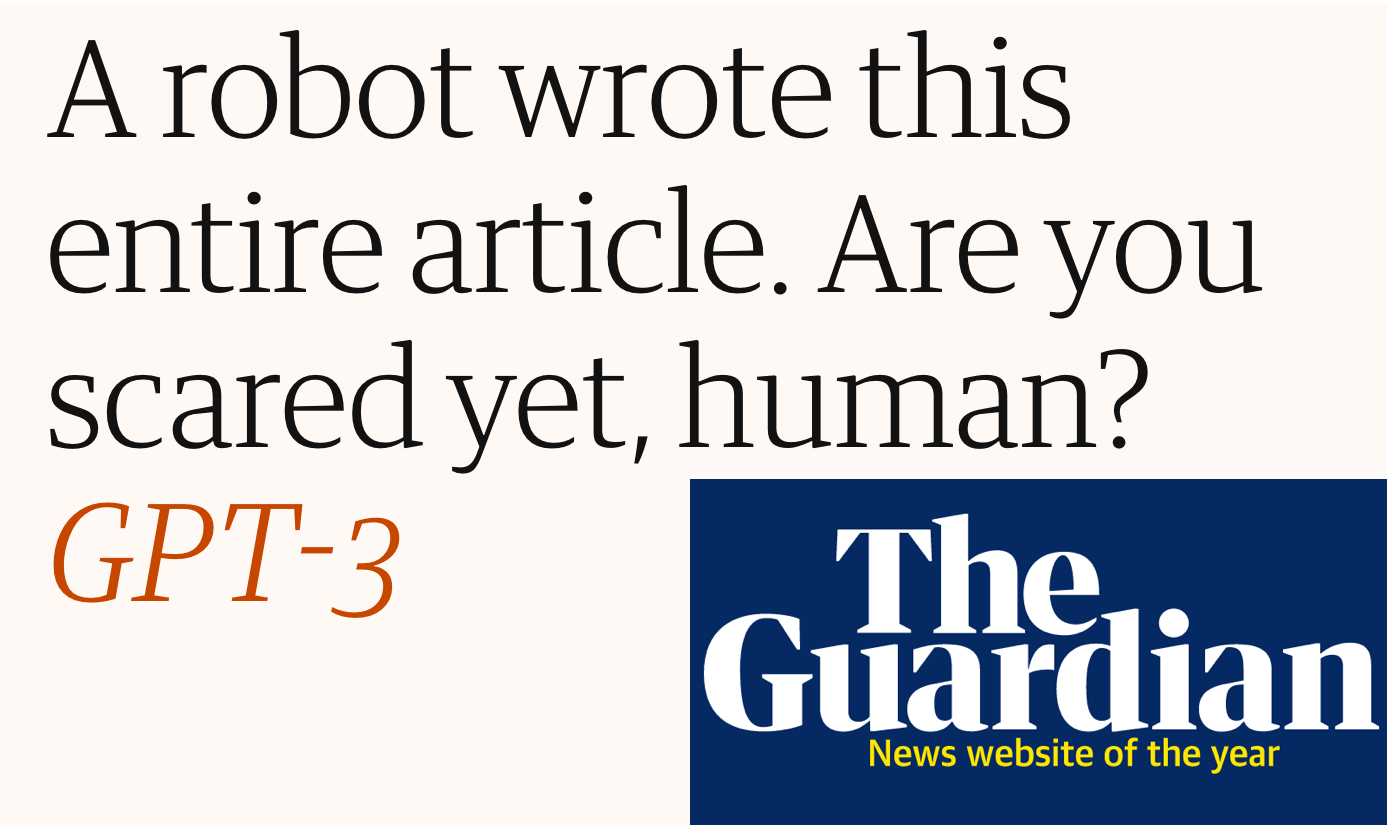
\includegraphics[width=0.4\columnwidth]{figures/guardian.png}};}
        % \uncover<3->{\node[xshift=-3cm,yshift=0cm] at (current page.center) {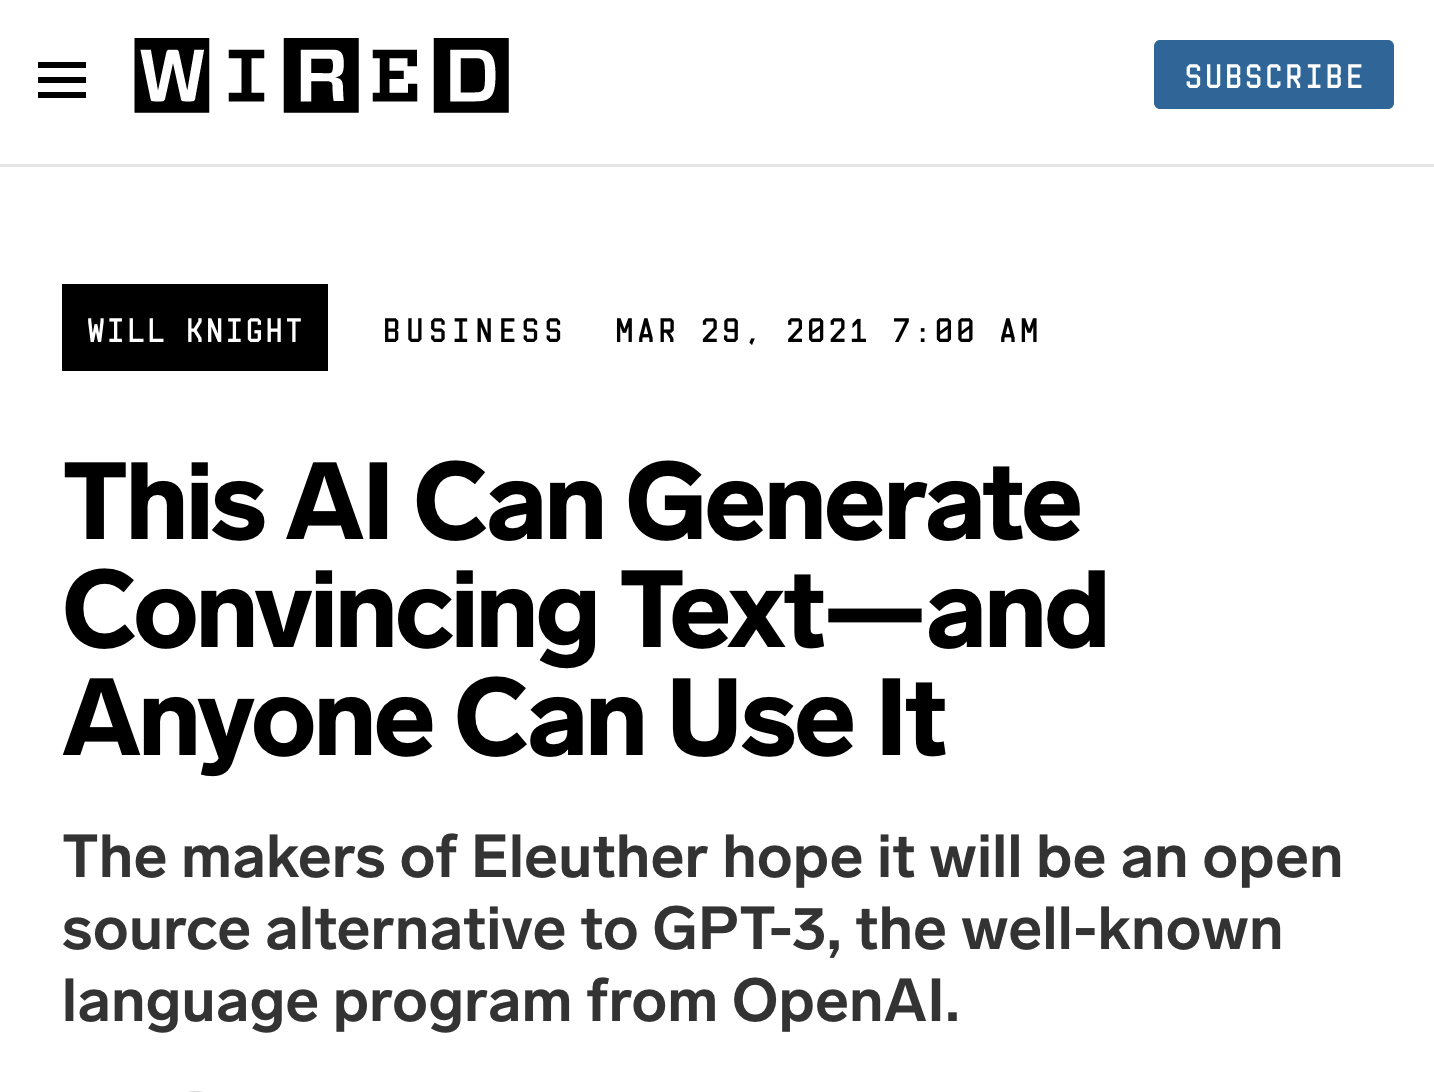
\includegraphics[width=0.4\columnwidth]{figures/wired.png}};}
        % \uncover<4->{\node[xshift=2cm,yshift=-2cm] at (current page.center) {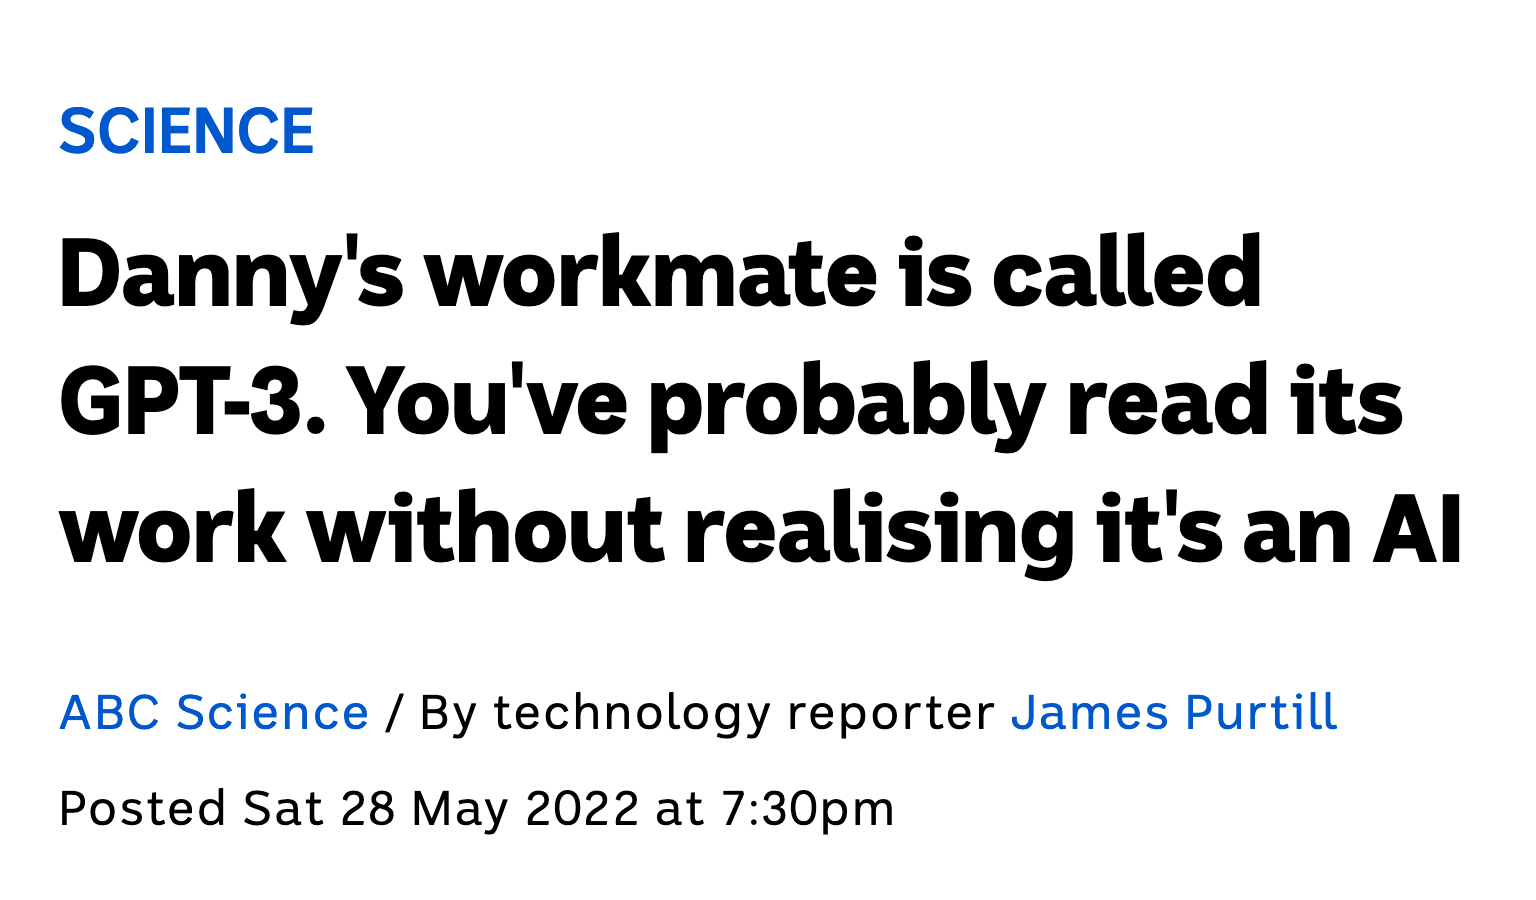
\includegraphics[width=0.5\columnwidth]{figures/abcscience.png}};}
        %\uncover<1->{\node[xshift=-3cm,yshift=-2cm] at (current page.center) {\fcolorbox{black}{black}{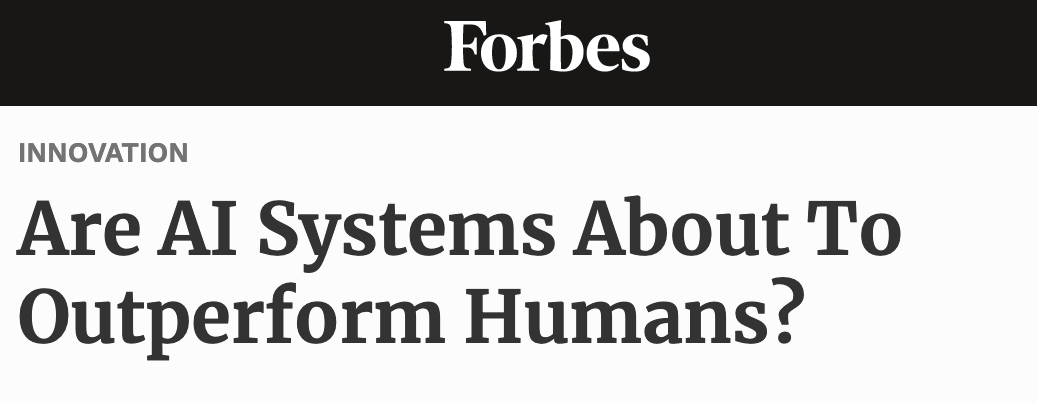
\includegraphics[width=0.5\columnwidth]{figures/forbes1.png}}};}
        \uncover<1->{\node[xshift=-3.5cm,yshift=1cm] at (current page.center) {\fcolorbox{black}{black}{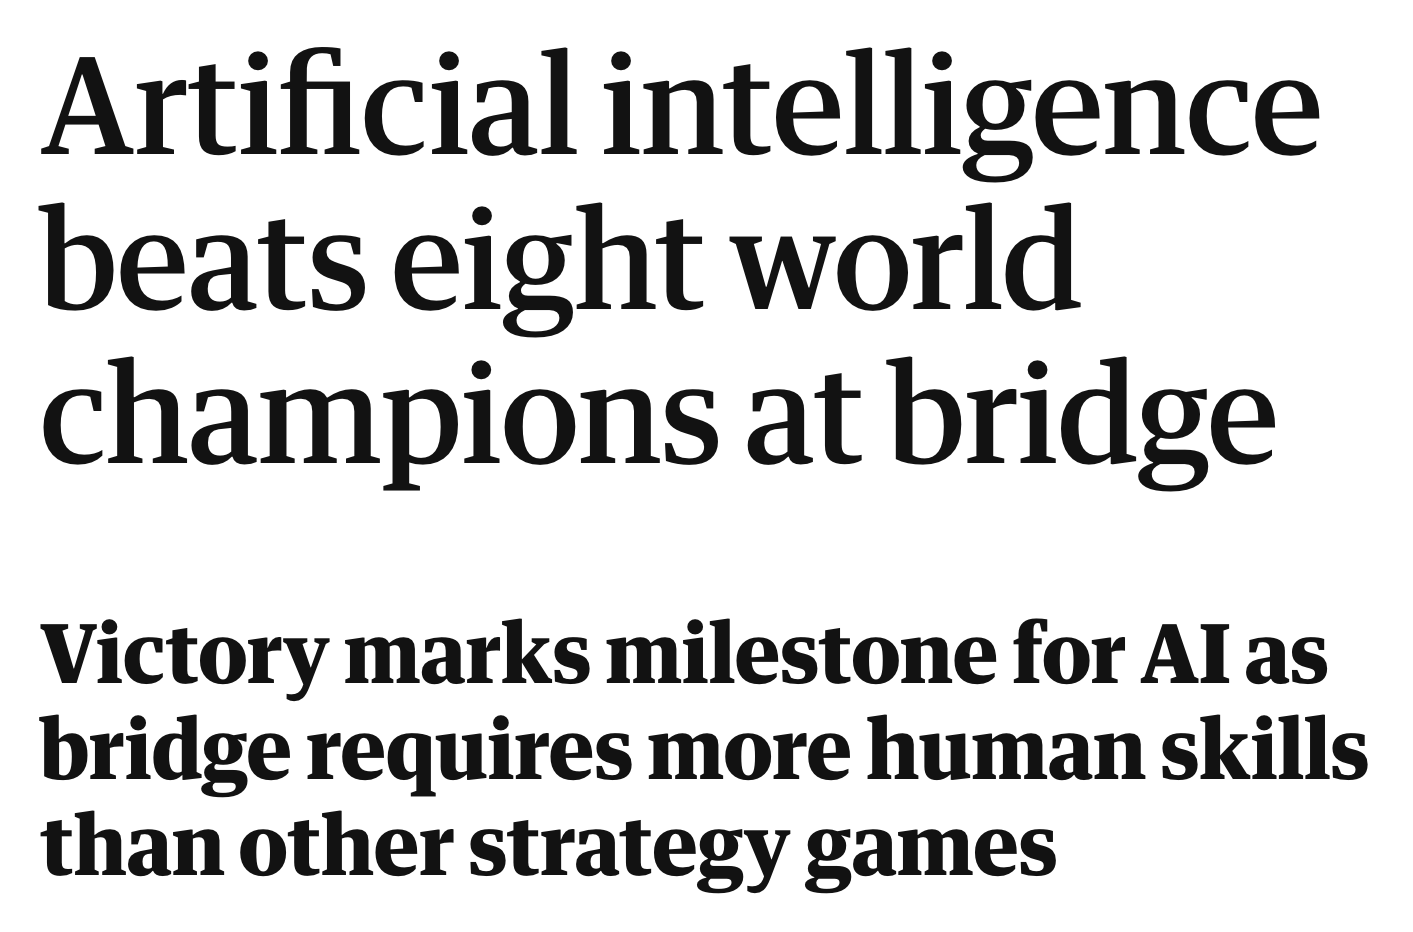
\includegraphics[width=0.5\columnwidth]{figures/bridge.png}}};}
        \uncover<2->{\node[xshift=3.5cm,yshift=-1cm] at (current page.center) {\fcolorbox{black}{black}{
\includegraphics[width=0.5\columnwidth]{figures/cancer.png}}};}
        \uncover<3->{\node[xshift=0cm,yshift=0cm] at (current page.center) {\fcolorbox{black}{black}{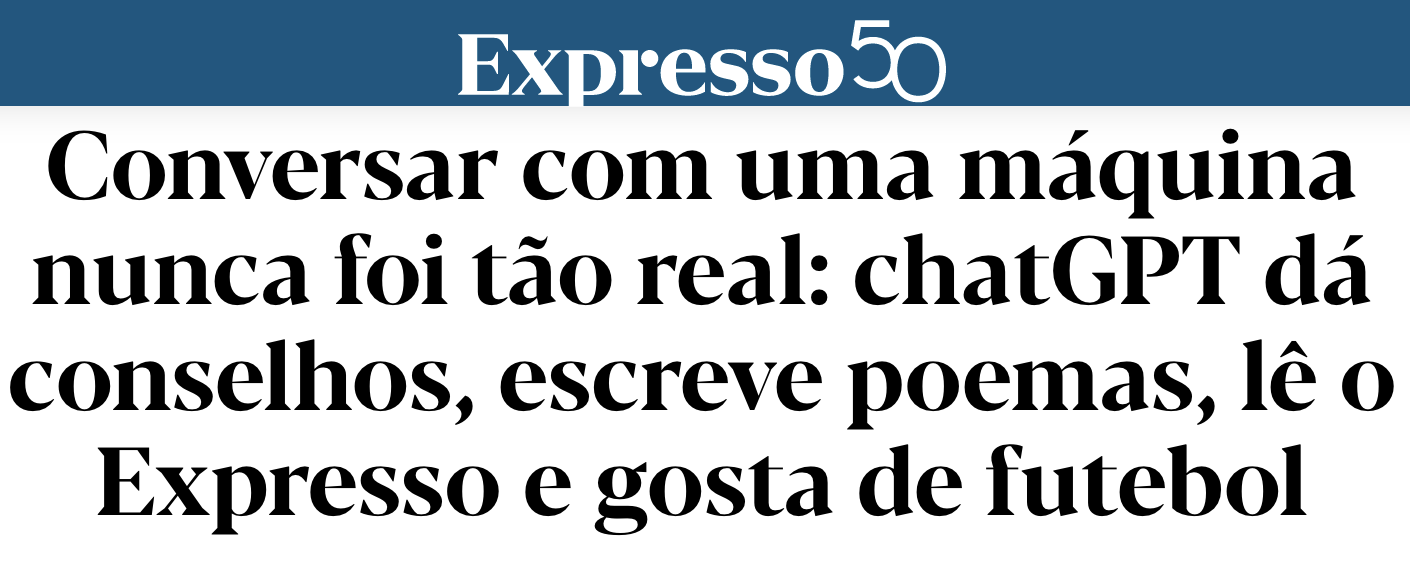
\includegraphics[width=0.7\columnwidth]{figures/expresso.png}}};}
    \end{tikzpicture}
\end{frame}

\begin{frame}
    \frametitle{Limitações}
    \begin{itemize}
        \uncover<2->{\item Quantidade de dados necessários}
              \uncover<3->{\item Dificuldade de interpretar os resultados}
              \uncover<4->{\item Quantidade de recursos computacionais necessários}
    \end{itemize}
\end{frame}

\begin{frame}
    \frametitle{Limitações}
    \fboxrule=2pt%border thickness
    \begin{tikzpicture}[remember picture,overlay]
        % \uncover<1->{\node[xshift=-3cm,yshift=0cm] at (current page.center) {\fcolorbox{black}{black}{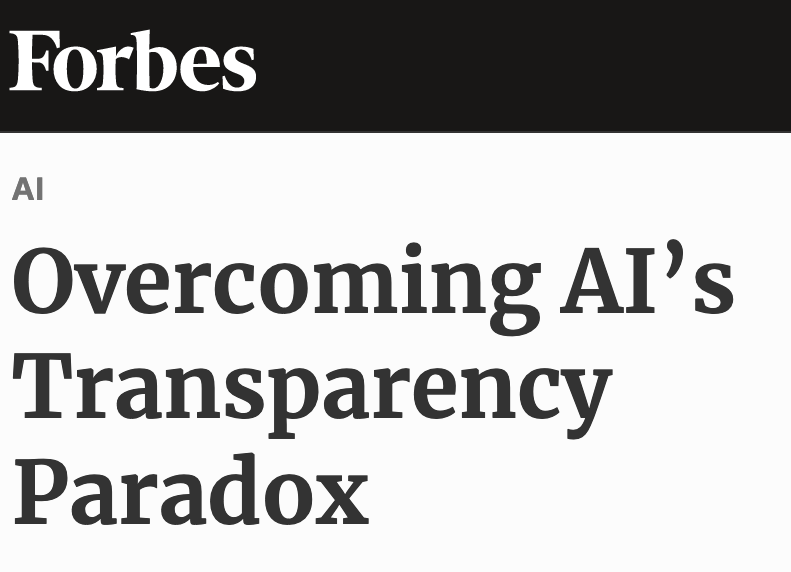
\includegraphics[width=0.4\columnwidth]{figures/transparency.png}}};}
        \uncover<1->{\node[xshift=2cm,yshift=-2cm] at (current page.center) {\fcolorbox{black}{black}{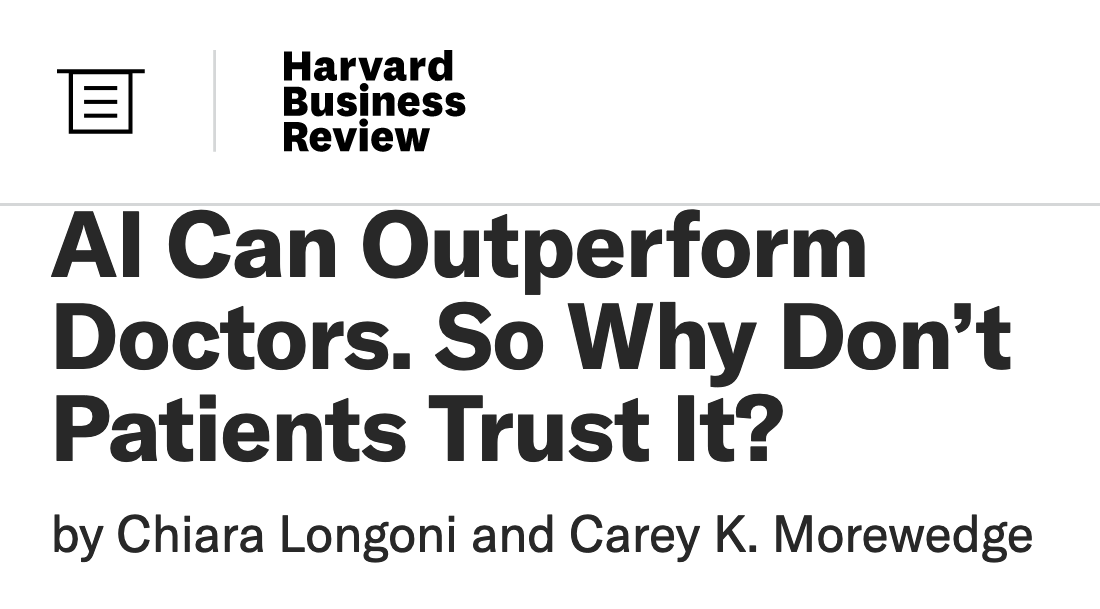
\includegraphics[width=0.5\columnwidth]{figures/patientstrust.png}}};}
        \uncover<2->{\node[xshift=3cm,yshift=1cm] at (current page.center) {\fcolorbox{black}{black}{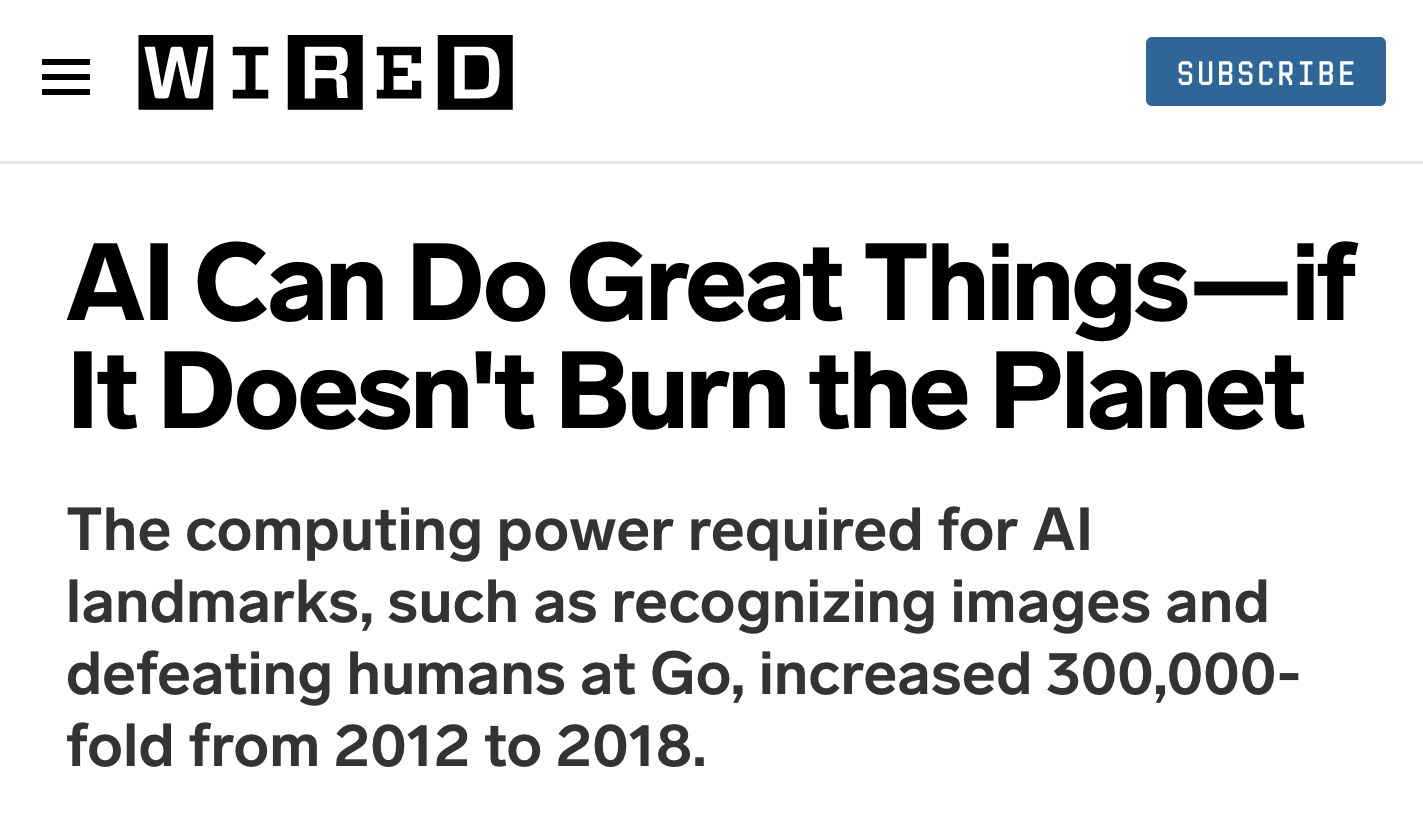
\includegraphics[width=0.4\columnwidth]{figures/climate.png}}};}
        \uncover<3->{\node[xshift=-2cm,yshift=-1cm] at (current page.center) {\fcolorbox{black}{black}{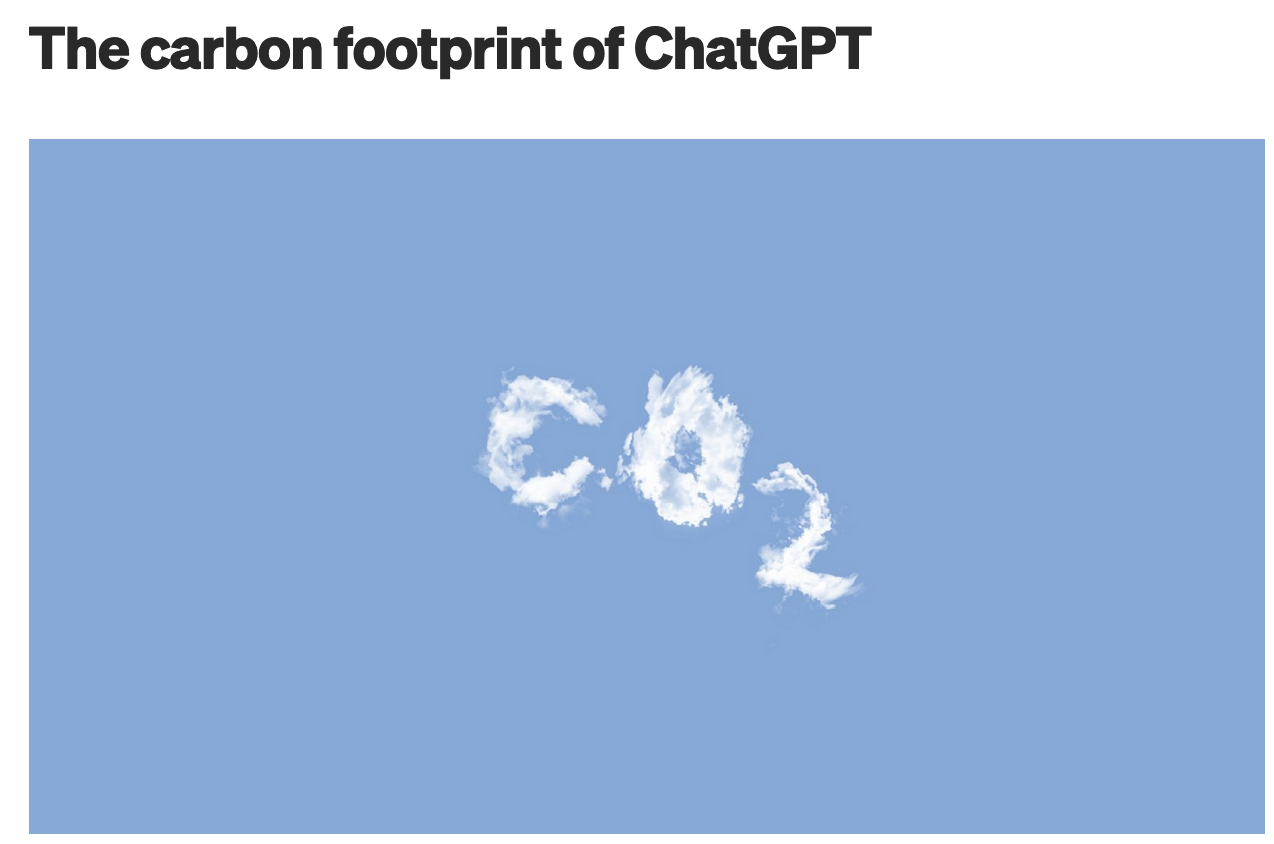
\includegraphics[width=0.5\columnwidth]{figures/footprintchatgpt.png}}};}
    \end{tikzpicture}
\end{frame}

\begin{frame}
    \frametitle{Objetivos do trabalho}
    \begin{tikzpicture}[remember picture, overlay]
        \node[font={\color{myfg}\usebeamerfont{title}},align=center]
        at ($(current page.center) + (0, 1.0)$) {Modelos Neuronais};
        \node[font={\color{myfg}\usebeamerfont{title}},align=center]
        at ($(current page.center) + (0, 0.0)$) {mais \only<2->{{\color{myDarkYellow} Transparentes}}\only<1>{Transparentes} e \only<3->{{\color{myDarkYellow} Compactos}}\only<1-2>{Compactos}};
        \node[font={\color{myfg}\usebeamerfont{title}},align=center]
        at ($(current page.center) + (0, -1.0)$) {usando \only<4->{{\color{tPeony} Esparsidade}}\only<1-3>{Esparsidade}};
    \end{tikzpicture}
\end{frame}

% \begin{frame}
%     \frametitle{Publicações}
%     \fontsize{12pt}{15}\selectfont

%     \begin{itemize}
%               \uncover<2->{\item Adaptively Sparse Transformers
%               \begin{itemize}
%                   \item {\color{tPeony} esparsidade adaptativa}
%                   \item {\color{myDarkYellow} objetivo de obter maior transparência}
%                   \item Apresentado oralmente no EMNLP 2019
%               \end{itemize}
%               }

%               \vspace{0.3cm}
%               \uncover<3->{\item Efficient Marginalization of Discrete Latent Variables with Sparsity
%               \begin{itemize}
%                   \item {\color{tPeony} aprendizagem da esparsidade}
%                   \item {\color{myDarkYellow} objetivo de compressão dos modelos}
%                   \item Publicação \emph{Spotlight} na NeurIPS 2020
%               \end{itemize}
%               }
%     \end{itemize}
% \end{frame}

% \section{A Simple and Effective Approach to APE with Transfer Learning}

% \begin{frame}
%     \frametitle{A bit of context on Transformers}

%     \fontsize{12pt}{15}\selectfont
%     \only<1-4>{\cornercite{transf}}
%     \only<5->{\cornercite{devlin2018bert}}
%     \begin{columns}
%         \uncover<1->{
%         \hspace{2mm}\vspace{-1cm}\begin{column}{0.6\columnwidth}
%             What if... Attention is all you need? \\
%             \vspace{0.5cm}
%             }
%             \uncover<2->{
%                 {\color{myDarkYellow} Key idea:} Let's mainly use attention mechanisms!
%                 \vspace{0.25cm}
%             }
%             \begin{itemize}
%                 \uncover<3->{\item Do attention with multiple heads (i.e. attention mechanisms in parallel)}
%                       \uncover<4->{\item ... and do it through several layers}
%                       \uncover<5->{\item Inspiration for big general-purpose models like BERT and GPT-3!}
%             \end{itemize}
%         \end{column}

%         \begin{column}{0.39\columnwidth}
%             \vspace{-1.5cm}
%             \only<1-2>{
%                 \begin{center}
%                     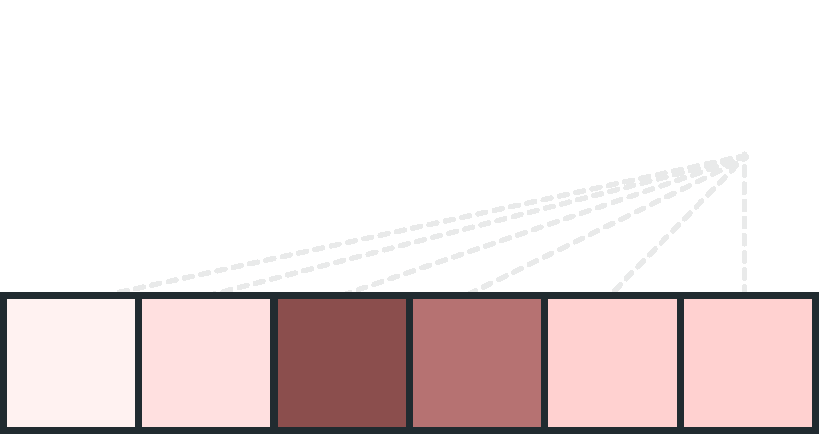
\includegraphics[width=0.8\columnwidth]{figures/single_head.pdf}
%                 \end{center}
%             }
%             \only<3>{
%                 \begin{center}
%                     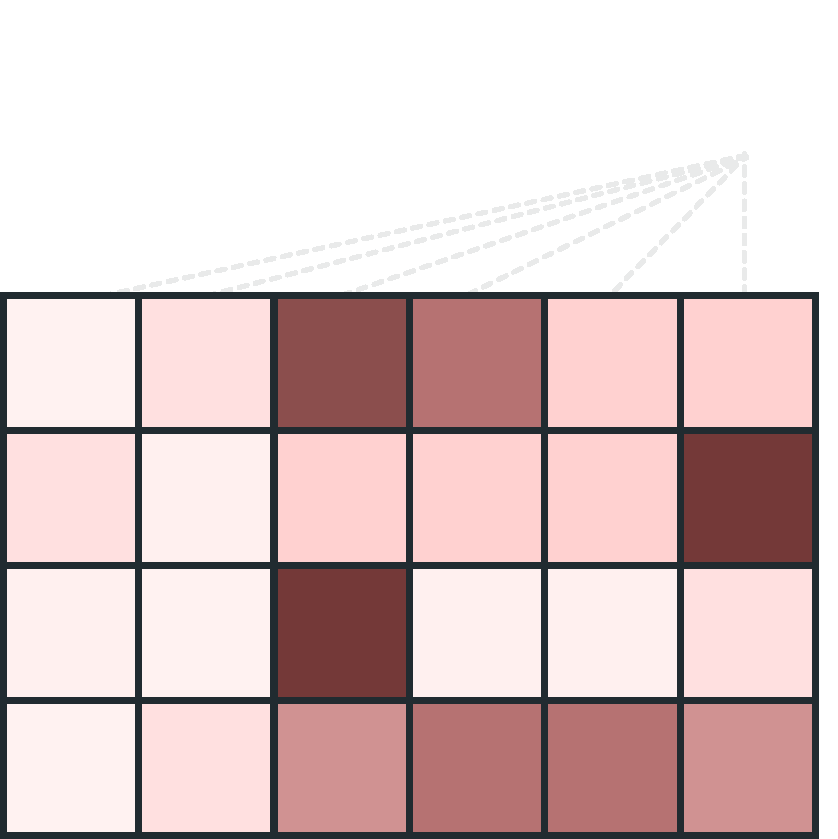
\includegraphics[width=0.8\columnwidth]{figures/multiple_heads.pdf}
%                 \end{center}
%             }
%             \only<4->{
%                 \begin{center}
%                     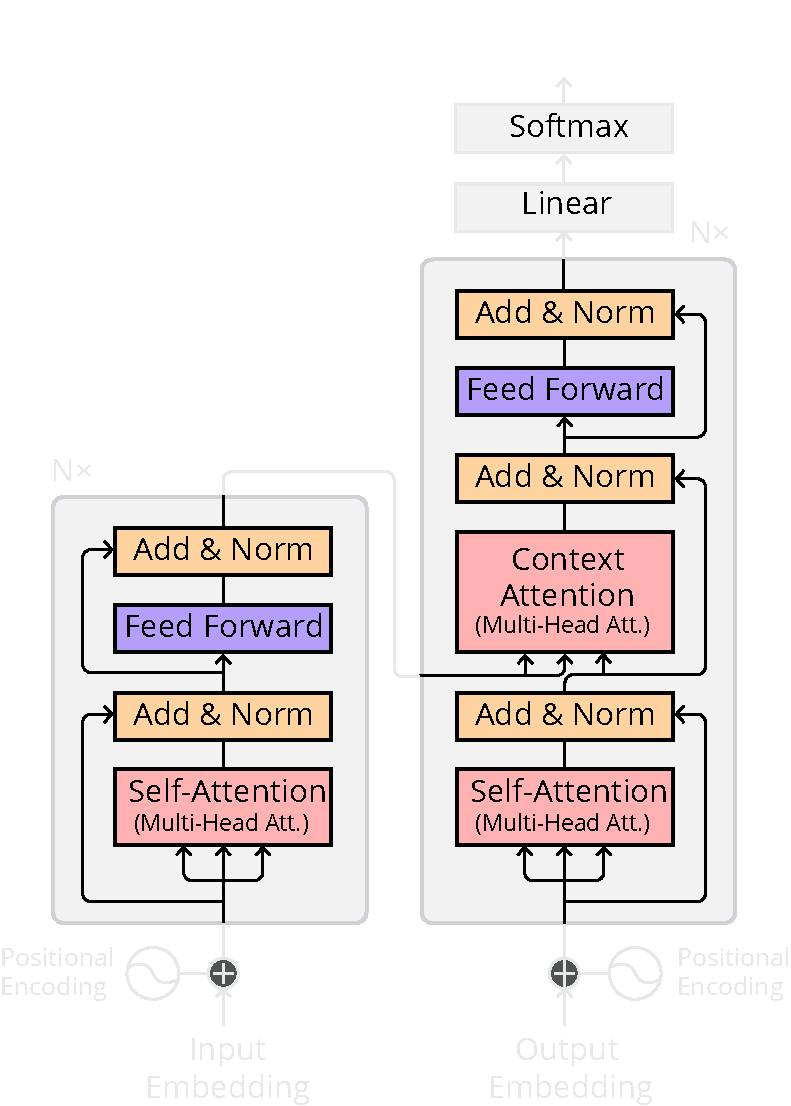
\includegraphics[width=0.8\columnwidth]{figures/transformer_mybg}
%                 \end{center}
%             }
%         \end{column}

%         \begin{tikzpicture}[remember picture, overlay]
%             \uncover<6->{\node[xshift=3cm,yshift=0cm] at (current page.center) {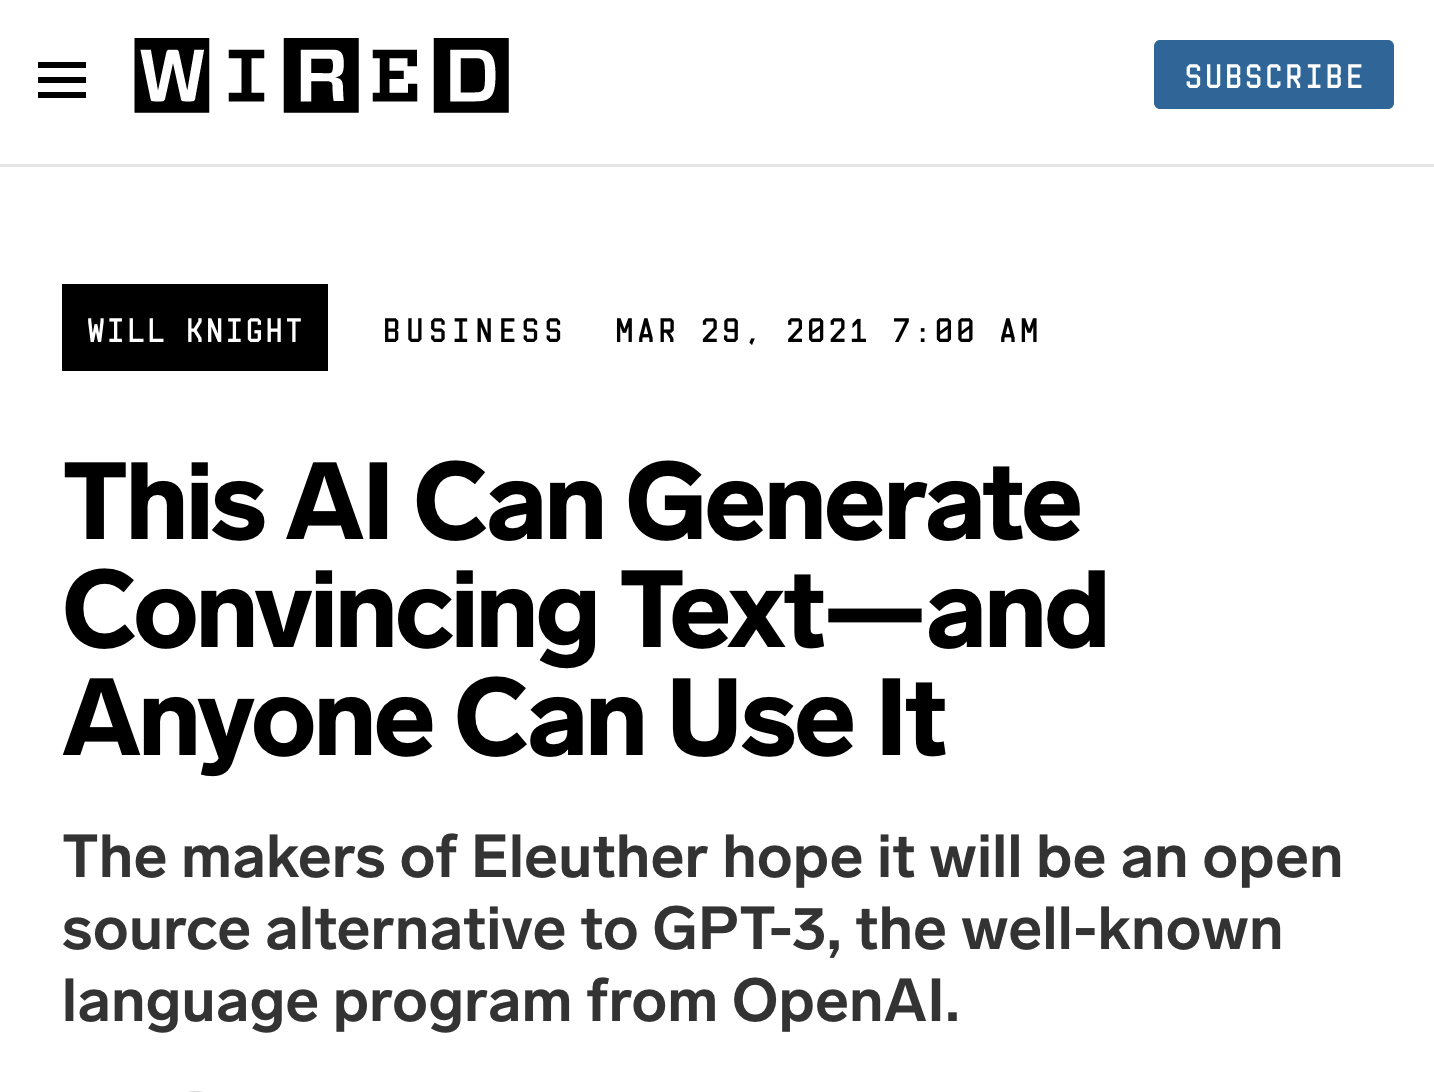
\includegraphics[width=0.4\columnwidth]{figures/wired.png}};}
%         \end{tikzpicture}
%     \end{columns}

% \end{frame}

% \begin{frame}
%     \frametitle{What is APE?}
%     \fontsize{12pt}{15}\selectfont
%     \centering
%     \begin{tikzpicture}[remember picture, overlay]
%         \uncover<2->{\node[xshift=0cm,yshift=1.7cm] at (current page.center) {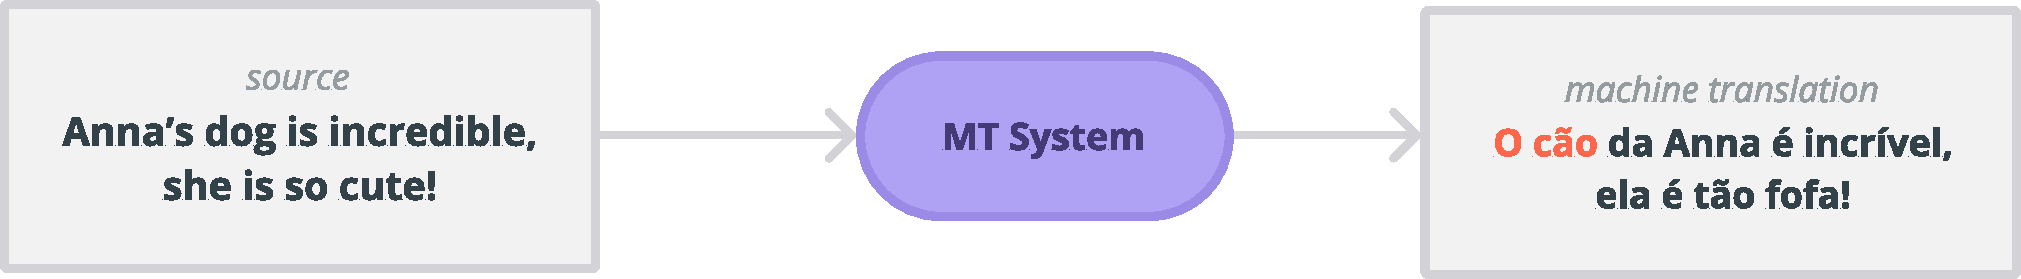
\includegraphics[width=0.7\columnwidth]{figures/mt.pdf}};}
%         \uncover<3->{\node[xshift=0cm,yshift=-1.3cm] at (current page.center) {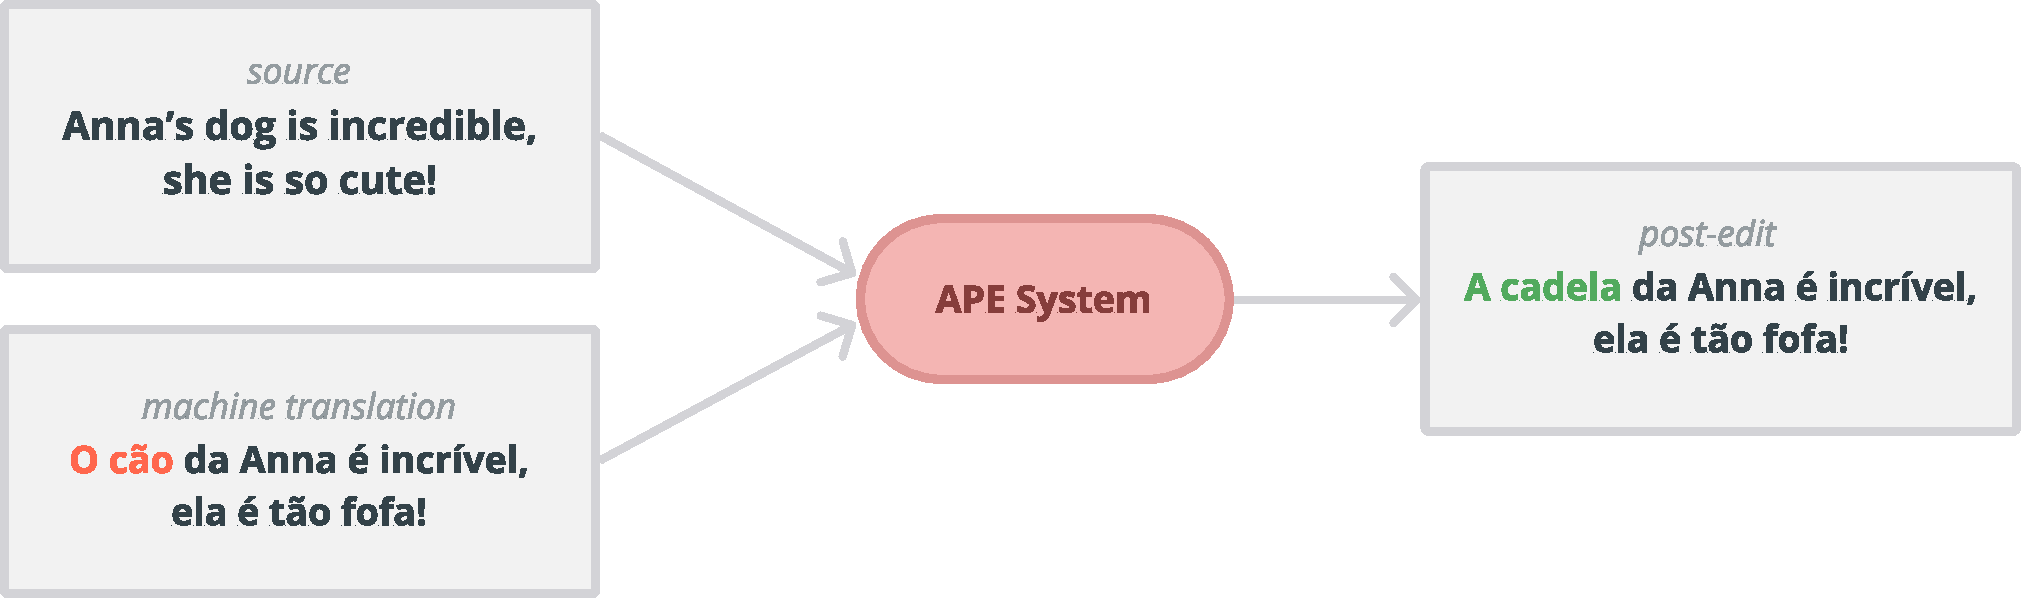
\includegraphics[width=0.7\columnwidth]{figures/ape.pdf}};}
%     \end{tikzpicture}
%     \vspace{5cm}
%     \begin{itemize}
%         \uncover<4->{\item[] {\color{myDarkYellow} Challenge:} APE data is very scarce! Need to create artificial data.}
%     \end{itemize}
% \end{frame}

% \begin{frame}
%     \frametitle{BERT for APE}

%     \fontsize{12pt}{15}\selectfont
%     %\cornercite{transf}
%     \begin{columns}
%         \uncover<1->{
%         \hspace{2mm}\vspace{-1cm}\begin{column}{0.55\columnwidth}
%             }
%             \uncover<2->{
%                 {\color{myDarkYellow} Key idea:} Use BERT to do APE \quad\emoji{palms}
%                 \vspace{0.25cm}
%             }
%             \begin{itemize}
%                 \uncover<3->{\item Prior to this work, BERT was mainly used for simple classification tasks}
%                       \uncover<4->{\item We introduced an effective method to use BERT in a generation task (APE)}
%                       \uncover<5->{\item Smart parameter sharing between encoder and decoder}
%             \end{itemize}
%         \end{column}

%         \begin{column}{0.4\columnwidth}
%             \vspace{-1.5cm}
%             \begin{center}
%                 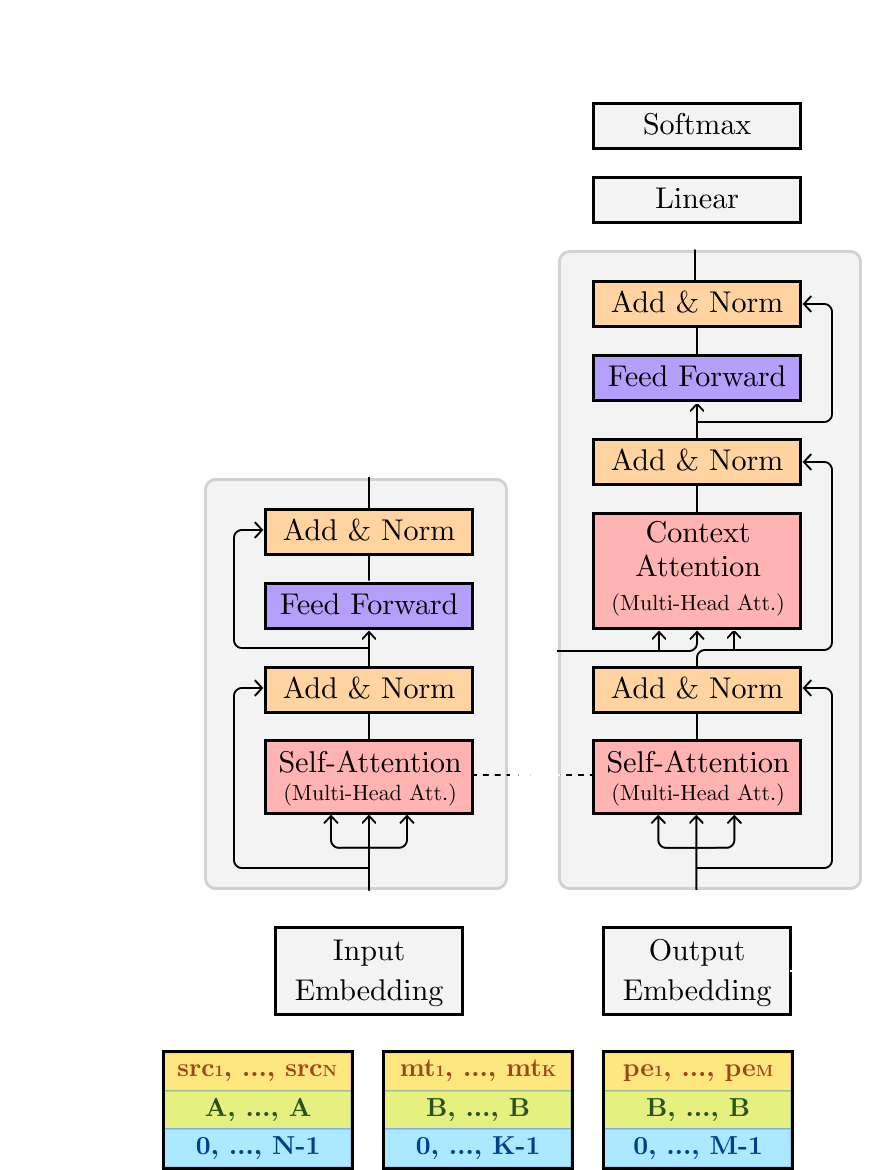
\includegraphics[width=0.8\columnwidth]{figures/bert-ape-2x.png}
%                 \tikz[baseline,remember picture]{\node[anchor=base] (t1){};}
%             \end{center}
%         \end{column}
%     \end{columns}
% \end{frame}

% \begin{frame}
%     \frametitle{Key results}
%     \uncover<2-3>{\cornercite{junczys2018ms}}
%     \centering

%     \vspace{-1.5cm}
%     \begin{tabular}{lrr}
%         \toprule
%         model (data size)
%          & TER$\downarrow$        & BLEU$\uparrow$                                  \\
%         \midrule
%         mt baseline
%          & 24.48                  & 62.49\phantom{i}                                \\
%         \uncover<2->{dual-source transformer (8M)
%          & {\color{tGreen} 18.10} & {\color{tGreen} 71.72}                        } \\
%         \uncover<3->{dual-source transformer (23K)
%          & {\color{tRed} 27.73}   & {\color{tRed} 59.78}                        }   \\
%         \uncover<4->{ours (23K)
%          & {\color{tGreen} 19.03} & {\color{tGreen} 70.66} }                        \\
%         \uncover<5->{ours (8M)
%          & {\color{tGreen} 17.26} & {\color{tGreen} 73.42} }                        \\
%         \bottomrule
%     \end{tabular}
% \end{frame}

% \begin{frame}
%     \frametitle{Key takeaways}
%     \uncover<4>{\cornercite{lee2020POSTECHETRISubmissionWMT2020}}
%     \begin{itemize}
%         \uncover<2->{\item One of pioneers in using pre-trained Transformer encoders for a generation task}
%               \uncover<3->{\item Massive improvement in low-resource scenario ({\color{myDarkYellow} data-efficiency})}
%               \uncover<4->{\item Steered SOTA of APE towards using {\color{tPeony} weak supervision} through pre-trained models}
%     \end{itemize}
% \end{frame}

\section{Adaptively Sparse Transformers}

\begin{frame}
    \frametitle{Tornar a rede esparsa}
    \fontsize{12pt}{15}\selectfont
    \begin{columns}
        \begin{column}{0.6\columnwidth}
            \begin{itemize}
                \uncover<1->{\item[] LMs usam representações {\color{myDarkYellow} densas}.}
            \end{itemize}

            \bigskip

            \begin{itemize}
                \item[]<2-> A nossa solução foi {\color{tPeony} esparsificar}:
            \end{itemize}

            \begin{quote}
                {\normalfont
                    \begin{itemize}
                        \only<2>{\item interpretabilidade} % sparse connections allow to be sure about which model representations were used to make a prediction
                        \only<2>{\item descobrir estruturas linguísticas} % we can redesign components based on what we find with sparsity
                    \end{itemize}}
            \end{quote}
        \end{column}

        \begin{column}{0.39\columnwidth}

            \vspace{-1.5cm}
            \only<1>{
            \begin{center}
                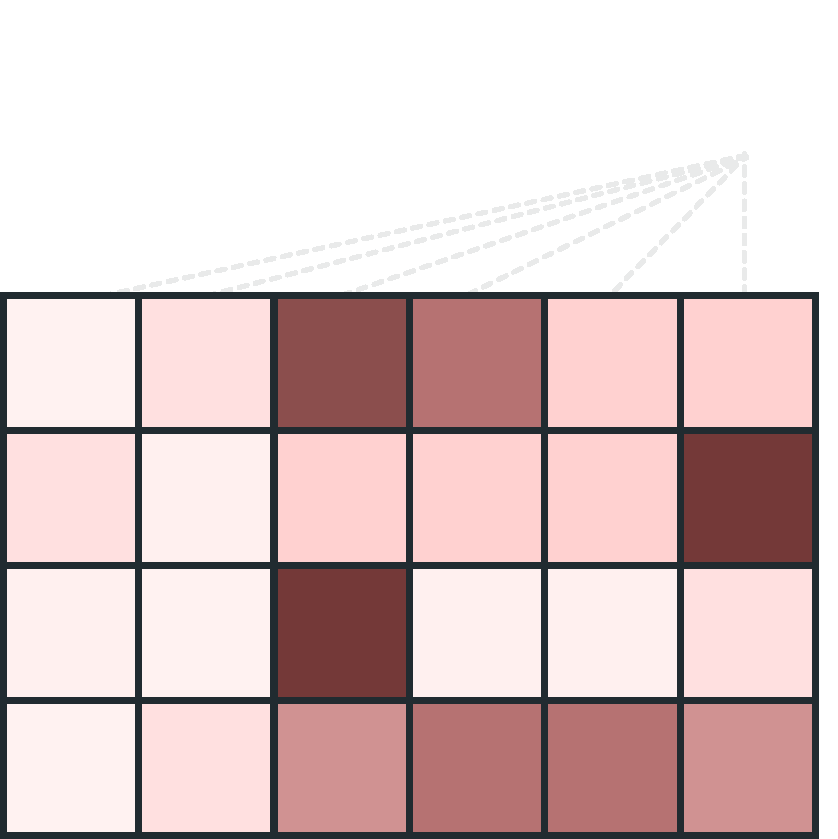
\includegraphics[width=0.8\columnwidth]{figures/multiple_heads.pdf}
            \end{center}
            }
            \only<2->{
            \begin{center}
                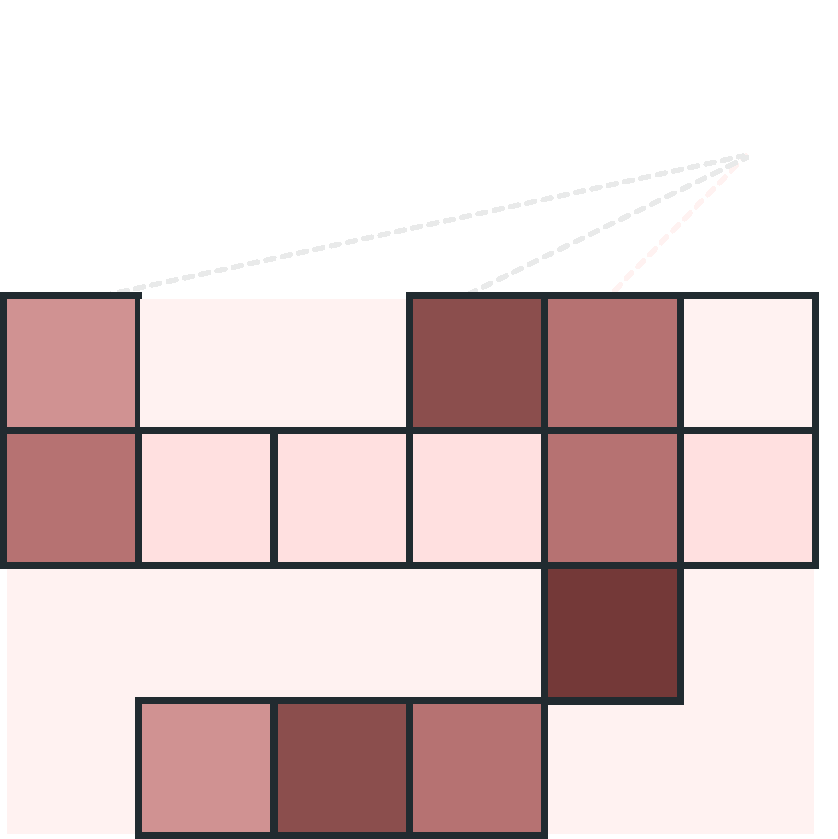
\includegraphics[width=0.8\columnwidth]{figures/adaptive_sparsity.pdf}
            \end{center}
            }
        \end{column}
    \end{columns}
\end{frame}

% \begin{frame}
%     \frametitle{
%         \only<2->{{\color{myDarkYellow}Adaptively}} \only<1->{{\color{colorEntmax}Sparse}} \uncover<1->{Transformers}}

%     \only<1-4>{
%         \fontsize{12pt}{15}\selectfont
%         \cornercite{transf}
%         \begin{columns}
%             \hspace{2mm}\vspace{-1cm}\begin{column}{0.55\columnwidth}
%                 In each attention head:
%                 \begin{equation*}
%                     \bar{\matr{V}}  = \softmax\left(\frac{\matr{Q}\matr{K}^\top}{\sqrt{d_k}}\right)\matr{V}.
%                 \end{equation*}
%                 \uncover<2-4>{Attention in three places:
%                 \begin{itemize}
%                     \item Self-attention in the encoder\tikz[remember picture]{\node[coordinate] (n1) {};}}
%                           \uncover<3-4>{\item Self-attention in the decoder\tikz[remember picture]{\node[coordinate] (n2) {};}}
%                           \uncover<4>{\item Contextual attention\tikz[remember picture]{\node[coordinate] (n3) {};}}
%                 \end{itemize}
%             \end{column}
%             \begin{column}{0.4\columnwidth}
%                 \vspace{-2cm}
%                 \begin{center}
%                     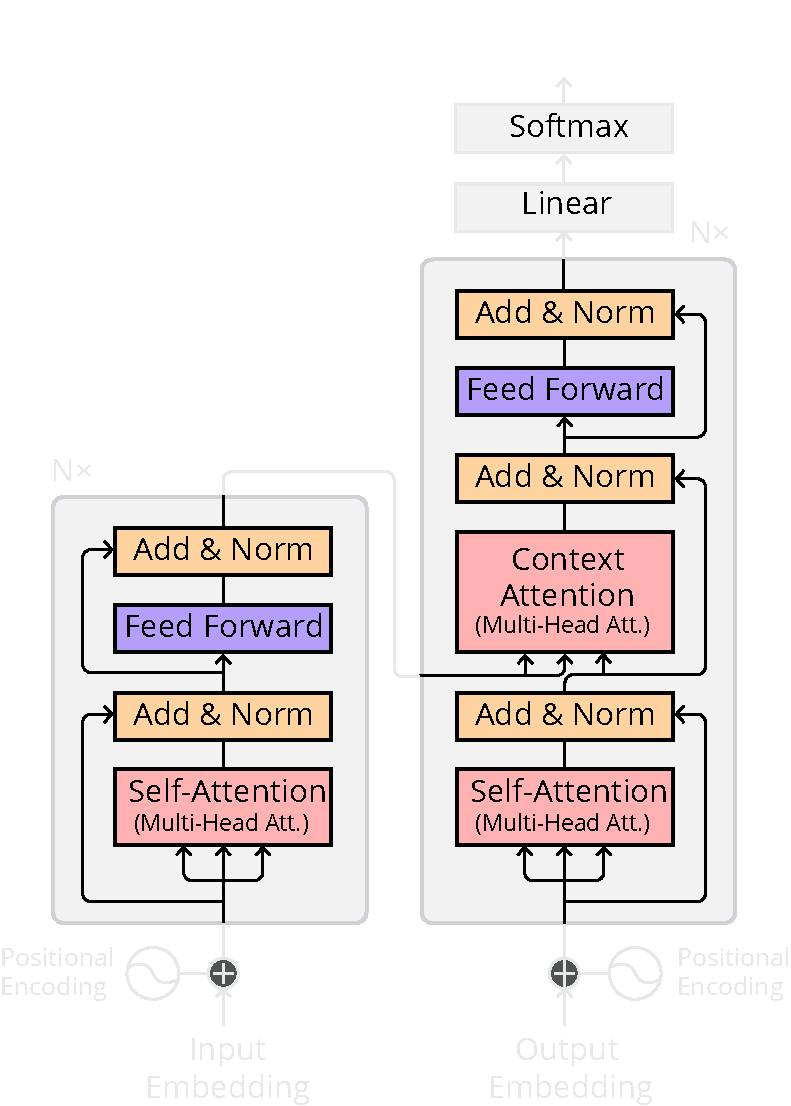
\includegraphics[width=0.9\columnwidth]{figures/transformer_mybg}
%                     \tikz[baseline,remember picture]{\node[anchor=base] (t1){};}
%                 \end{center}
%             \end{column}
%         \end{columns}

%     }

% \begin{itemize}
%     \item[]\uncover<1->{
%         {\color{colorEntmax} Ideia-chave:} usar uma função esparsa nas componentes do modelo
%     }

%     \bigskip

%     \item[]\uncover<2->{
%         {\color{myDarkYellow} Outra ideia-chave:}
%         usar uma função esparsa mas adaptável e que o modelo aprende a gerir!
%     }
% \end{itemize}

% \end{frame}

% \begin{frame}%
%     \frametitle{What is softmax?}%
%     \centering \fontsize{12pt}{15}\selectfont
%     Softmax exponentiates and normalizes:

%     \begin{center}
%         $\displaystyle
%             \left[\softmax(\xx)\right]_i \defeq \frac{\exp \left(\xx_i\right)}{\sum_j \exp \left(\xx_j\right)}$
%     \end{center}

%     \bigskip

%     \uncover<2->{
%         {\color{myDarkYellow} It's fully dense: $\softmax(\vectsymb{z}) > \vect{0}$}}

% \end{frame}

% \begin{frame}{$\alpha$-entmax}
%     \cornercite{Peters2019ACL}
%     \vspace{-1cm}
%     \fontsize{12pt}{15}\selectfont
%     \begin{itemize}
%         \item[] Parametrized by {\color{tPeony}$\alpha \ge 0$}:
%     \end{itemize}
%     \bigskip
%     % \begin{center}
%     % $\displaystyle
%     % \Omega_{{\color{tPeony}\alpha}}(\vectsymb{p}) \defeq 
%     % \left\{
%     % \begin{array}{ll}
%     % \frac{1}{\alpha(\alpha-1)} \left(1 - \sum_{i=1}^K p_i^{\alpha}\right) & \text{if $\alpha \ne 1$}\\
%     % \sum_{i=1}^K p_i\log p_i & \text{if $\alpha = 1$.}
%     % \end{array}
%     % \right.$
%     % \end{center}
%     % \bigskip
%     \begin{itemize}
%         \uncover<2->{\item {\bf Argmax} corresponds to {\color{tPeony}$\alpha \rightarrow \infty$}}
%               \uncover<3->{\item {\bf Softmax} amounts to {\color{tPeony}$\alpha \rightarrow 1$}}
%     \end{itemize}
%     \bigskip
%     \begin{itemize}
%         \uncover<4->{\item[] {\color{myDarkYellow} Key result:} {\bf can be sparse for $\alpha > 1$}, propensity for sparsity increases with $\alpha$.}
%     \end{itemize}

% \end{frame}

% \begin{frame}
%     \centering
%     % This file was created by tikzplotlib v0.8.5.
\begin{tikzpicture}

\definecolor{color0}{rgb}{0.63921568627451,0.658823529411765,0.635294117647059}
\definecolor{color1}{rgb}{0,0.709803921568627,0.83921568627451}
\definecolor{color2}{rgb}{0.552941176470588,0.827450980392157,0.780392156862745}
\definecolor{color3}{rgb}{0.890196078431372,0.384313725490196,0.486274509803922}
\definecolor{color4}{rgb}{0.866666666666667,0.850980392156863,0.72156862745098}
\definecolor{color5}{rgb}{0.466666666666667,0.498039215686275,0.458823529411765}

\begin{axis}[
width=0.9\columnwidth,
height=0.8\paperheight, 
axis line style={color0},
legend cell align={left},
legend style={
    nodes={scale=0.8, transform shape}, at={(0.97,0.3)}, anchor=east, draw=white!80.0!black, fill=myfg!30!mybg, fill opacity=0.6, draw opacity=1,text opacity=1},
tick align=outside,
tick pos=left,
x grid style={white!69.01960784313725!black},
xlabel={t},
xmin=-4.18, xmax=4.18,
xtick style={color=color0},
y grid style={white!69.01960784313725!black},
ymin=-0.05, ymax=1.05,
ytick style={color=color0}
]
\addplot [ultra thick, color1, dotted, visible on=<1->]
table {%
-3.8 0.0218797076995784
-3.79239239239239 0.0220431176990893
-3.78478478478478 0.0222077204139333
-3.77717717717718 0.0223735241350471
-3.76956956956957 0.02254053720296
-3.76196196196196 0.022708768011741
-3.75435435435435 0.0228782250060016
-3.74674674674675 0.0230489166826131
-3.73913913913914 0.023220851591204
-3.73153153153153 0.0233940383338884
-3.72392392392392 0.0235684855654955
-3.71631631631632 0.0237442019927435
-3.70870870870871 0.0239211963765537
-3.7011011011011 0.0240994775315149
-3.69349349349349 0.0242790543250429
-3.68588588588589 0.0244599356792074
-3.67827827827828 0.0246421305693472
-3.67067067067067 0.024825648024818
-3.66306306306306 0.0250104971303179
-3.65545545545546 0.0251966870250253
-3.64784784784785 0.025384226902531
-3.64024024024024 0.0255731260121778
-3.63263263263263 0.0257633936578743
-3.62502502502502 0.0259550392000158
-3.61741741741742 0.0261480720531249
-3.60980980980981 0.0263425016898114
-3.6022022022022 0.0265383376372378
-3.59459459459459 0.0267355894793524
-3.58698698698699 0.0269342668562215
-3.57937937937938 0.0271343794663349
-3.57177177177177 0.0273359370623263
-3.56416416416416 0.0275389494565811
-3.55655655655656 0.0277434265178456
-3.54894894894895 0.0279493781717068
-3.54134134134134 0.0281568144020211
-3.53373373373373 0.0283657452511388
-3.52612612612613 0.0285761808185395
-3.51851851851852 0.0287881312622743
-3.51091091091091 0.0290016068001401
-3.5033033033033 0.0292166177060302
-3.4956956956957 0.0294331743149346
-3.48808808808809 0.0296512870195949
-3.48048048048048 0.0298709662726378
-3.47287287287287 0.0300922225854518
-3.46526526526527 0.0303150665293606
-3.45765765765766 0.0305395087354829
-3.45005005005005 0.0307655598945752
-3.44244244244244 0.0309932307575462
-3.43483483483483 0.0312225321345982
-3.42722722722723 0.0314534748988601
-3.41961961961962 0.0316860699806737
-3.41201201201201 0.0319203283729567
-3.4044044044044 0.032156261129298
-3.3967967967968 0.0323938793641164
-3.38918918918919 0.0326331942531791
-3.38158158158158 0.0328742170330385
-3.37397397397397 0.0331169590011706
-3.36636636636637 0.0333614315183326
-3.35875875875876 0.0336076460042998
-3.35115115115115 0.0338556139443042
-3.34354354354354 0.0341053468821192
-3.33593593593594 0.03435685642427
-3.32832832832833 0.0346101542421185
-3.32072072072072 0.034865252065515
-3.31311311311311 0.0351221616890269
-3.30550550550551 0.0353808949690087
-3.2978978978979 0.0356414638252814
-3.29029029029029 0.0359038802384934
-3.28268268268268 0.0361681562545827
-3.27507507507507 0.0364343039801273
-3.26746746746747 0.0367023355868511
-3.25985985985986 0.0369722633072921
-3.25225225225225 0.037244099439367
-3.24464464464464 0.0375178563423836
-3.23703703703704 0.0377935464408404
-3.22942942942943 0.0380711822199333
-3.22182182182182 0.0383507762319267
-3.21421421421421 0.0386323410899314
-3.20660660660661 0.0389158894709048
-3.198998998999 0.0392014341166009
-3.19139139139139 0.0394889878314867
-3.18378378378378 0.0397785634836498
-3.17617617617618 0.0400701740066303
-3.16856856856857 0.0403638323950521
-3.16096096096096 0.0406595517095343
-3.15335335335335 0.0409573450731743
-3.14574574574575 0.0412572256742813
-3.13813813813814 0.0415592067636878
-3.13053053053053 0.0418633016570484
-3.12292292292292 0.0421695237325527
-3.11531531531532 0.0424778864341914
-3.10770770770771 0.0427884032685098
-3.1001001001001 0.0431010878055185
-3.09249249249249 0.0434159536806046
-3.08488488488488 0.0437330145911802
-3.07727727727728 0.0440522842995363
-3.06966966966967 0.0443737766308916
-3.06206206206206 0.0446975054743283
-3.05445445445445 0.0450234847837648
-3.04684684684685 0.0453517285739309
-3.03923923923924 0.0456822509273209
-3.03163163163163 0.0460150659825459
-3.02402402402402 0.0463501879473853
-3.01641641641642 0.0466876310953057
-3.00880880880881 0.0470274097524212
-3.0012012012012 0.0473695383212204
-2.99359359359359 0.0477140312550073
-2.98598598598599 0.04806090307497
-2.97837837837838 0.0484101683697262
-2.97077077077077 0.0487618417802252
-2.96316316316316 0.0491159380177959
-2.95555555555556 0.0494724718522275
-2.94794794794795 0.0498314581153683
-2.94034034034034 0.0501929117043252
-2.93273273273273 0.0505568475735747
-2.92512512512512 0.0509232807408625
-2.91751751751752 0.0512922262859585
-2.90990990990991 0.0516636993482092
-2.9023023023023 0.0520377151280267
-2.89469469469469 0.0524142888878628
-2.88708708708709 0.0527934359508798
-2.87947947947948 0.0531751716960219
-2.87187187187187 0.0535595115677392
-2.86426426426426 0.053946471066972
-2.85665665665666 0.0543360657556165
-2.84904904904905 0.0547283112520736
-2.84144144144144 0.0551232232363988
-2.83383383383383 0.0555208174458155
-2.82622622622623 0.0559211096768649
-2.81861861861862 0.0563241157826499
-2.81101101101101 0.056729851673111
-2.8034034034034 0.0571383333191261
-2.7957957957958 0.0575495767440118
-2.78818818818819 0.0579635980288171
-2.78058058058058 0.0583804133139655
-2.77297297297297 0.0588000387892192
-2.76536536536537 0.0592224907082006
-2.75775775775776 0.0596477853717613
-2.75015015015015 0.0600759391386485
-2.74254254254254 0.0605069684218627
-2.73493493493493 0.0609408896875703
-2.72732732732733 0.0613777194546562
-2.71971971971972 0.0618174742956382
-2.71211211211211 0.062260170834864
-2.7045045045045 0.0627058257466367
-2.6968968968969 0.0631544557616842
-2.68928928928929 0.063606077654848
-2.68168168168168 0.0640607082564316
-2.67407407407407 0.0645183644439932
-2.66646646646647 0.0649790631438923
-2.65885885885886 0.0654428213314613
-2.65125125125125 0.0659096560319284
-2.64364364364364 0.066379584314756
-2.63603603603604 0.0668526232981398
-2.62842842842843 0.0673287901462386
-2.62082082082082 0.0678081020670497
-2.61321321321321 0.06829057631703
-2.60560560560561 0.0687762301921844
-2.597997997998 0.0692650810357034
-2.59039039039039 0.0697571462327773
-2.58278278278278 0.0702524432091021
-2.57517517517518 0.0707509894340488
-2.56756756756757 0.071252802414493
-2.55995995995996 0.0717578997003455
-2.55235235235235 0.0722662988807092
-2.54474474474474 0.072778017579887
-2.53713713713714 0.0732930734638156
-2.52952952952953 0.0738114842295847
-2.52192192192192 0.0743332676168075
-2.51431431431431 0.0748584413953959
-2.50670670670671 0.075387023372081
-2.4990990990991 0.0759190313845911
-2.49149149149149 0.076454483304089
-2.48388388388388 0.0769933970351715
-2.47627627627628 0.0775357905107235
-2.46866866866867 0.078081681692644
-2.46106106106106 0.0786310885735
-2.45345345345345 0.0791840291729984
-2.44584584584585 0.0797405215378729
-2.43823823823824 0.0803005837391156
-2.43063063063063 0.0808642338736056
-2.42302302302302 0.0814314900604077
-2.41541541541542 0.0820023704442239
-2.40780780780781 0.0825768931880155
-2.4002002002002 0.0831550764782652
-2.39259259259259 0.0837369385156147
-2.38498498498498 0.0843224975238593
-2.37737737737738 0.0849117717423827
-2.36976976976977 0.0855047794230473
-2.36216216216216 0.0861015388394116
-2.35455455455455 0.0867020682713393
-2.34694694694695 0.0873063860141924
-2.33933933933934 0.087914510372828
-2.33173173173173 0.0885264596632377
-2.32412412412412 0.0891422522103308
-2.31651651651652 0.0897619063436635
-2.30890890890891 0.0903854404000488
-2.3013013013013 0.0910128727192391
-2.29369369369369 0.091644221647602
-2.28608608608609 0.0922795055286687
-2.27847847847848 0.092918742706734
-2.27087087087087 0.0935619515296079
-2.26326326326326 0.094209150337922
-2.25565565565566 0.0948603574687727
-2.24804804804805 0.0955155912542545
-2.24044044044044 0.0961748700210421
-2.23283283283283 0.0968382120824677
-2.22522522522523 0.0975056357497986
-2.21761761761762 0.0981771593135052
-2.21001001001001 0.098852801056718
-2.2024024024024 0.0995325792460845
-2.19479479479479 0.10021651213119
-2.18718718718719 0.100904617942879
-2.17957957957958 0.101596914894943
-2.17197197197197 0.102293421176828
-2.16436436436436 0.102994154956395
-2.15675675675676 0.103699134373616
-2.14914914914915 0.104408377549139
-2.14154154154154 0.105121902561745
-2.13393393393393 0.105839727477795
-2.12632632632633 0.106561870314517
-2.11871871871872 0.107288349066146
-2.11111111111111 0.108019181685626
-2.1035035035035 0.108754386094593
-2.0958958958959 0.109493980167071
-2.08828828828829 0.110237981740711
-2.08068068068068 0.110986408606362
-2.07307307307307 0.111739278518368
-2.06546546546547 0.112496609167864
-2.05785785785786 0.113258418212891
-2.05025025025025 0.114024723249029
-2.04264264264264 0.114795541826045
-2.03503503503504 0.115570891431931
-2.02742742742743 0.116350789499589
-2.01981981981982 0.117135253406062
-2.01221221221221 0.117924300458695
-2.0046046046046 0.118717947908479
-1.996996996997 0.119516212937464
-1.98938938938939 0.120319112656411
-1.98178178178178 0.121126664111832
-1.97417417417417 0.121938884269009
-1.96656656656657 0.122755790029832
-1.95895895895896 0.123577398204778
-1.95135135135135 0.124403725537689
-1.94374374374374 0.125234788684354
-1.93613613613614 0.126070604216887
-1.92852852852853 0.126911188618487
-1.92092092092092 0.127756558290835
-1.91331331331331 0.128606729536149
-1.90570570570571 0.129461718567351
-1.8980980980981 0.130321541499894
-1.89049049049049 0.13118621435063
-1.88288288288288 0.132055753038175
-1.87527527527528 0.132930173371547
-1.86766766766767 0.133809491057758
-1.86006006006006 0.13469372169781
-1.85245245245245 0.135582880772085
-1.84484484484484 0.136476983660075
-1.83723723723724 0.13737604561675
-1.82962962962963 0.138280081778777
-1.82202202202202 0.139189107161791
-1.81441441441441 0.140103136659201
-1.80680680680681 0.141022185037897
-1.7991991991992 0.141946266927577
-1.79159159159159 0.142875396839867
-1.78398398398398 0.143809589140387
-1.77637637637638 0.144748858056768
-1.76876876876877 0.145693217683834
-1.76116116116116 0.146642681967916
-1.75355355355355 0.147597264715212
-1.74594594594595 0.148556979570884
-1.73833833833834 0.149521840043903
-1.73073073073073 0.150491859481172
-1.72312312312312 0.151467051070985
-1.71551551551552 0.152447427843341
-1.70790790790791 0.153433002670359
-1.7003003003003 0.154423788251378
-1.69269269269269 0.155419797119994
-1.68508508508509 0.156421041639324
-1.67747747747748 0.157427534000667
-1.66986986986987 0.158439286209903
-1.66226226226226 0.159456310100016
-1.65465465465465 0.160478617321037
-1.64704704704705 0.161506219329706
-1.63943943943944 0.16253912740589
-1.63183183183183 0.163577352624343
-1.62422422422422 0.164620905871167
-1.61661661661662 0.1656697978371
-1.60900900900901 0.166724039008795
-1.6014014014014 0.167783639669184
-1.59379379379379 0.168848609892329
-1.58618618618619 0.169918959543851
-1.57857857857858 0.170994698281474
-1.57097097097097 0.172075835540412
-1.56336336336336 0.173162380537527
-1.55575575575576 0.174254342268023
-1.54814814814815 0.175351729504056
-1.54054054054054 0.176454550787535
-1.53293293293293 0.177562814432604
-1.52532532532533 0.178676528512463
-1.51771771771772 0.179795700869748
-1.51011011011011 0.180920339105327
-1.5025025025025 0.182050450570817
-1.4948948948949 0.183186042379237
-1.48728728728729 0.184327121387525
-1.47967967967968 0.185473694199098
-1.47207207207207 0.186625767176986
-1.46446446446446 0.187783346403352
-1.45685685685686 0.188946437713144
-1.44924924924925 0.190115046670008
-1.44164164164164 0.191289178575399
-1.43403403403403 0.192468838454637
-1.42642642642643 0.193654031061913
-1.41881881881882 0.194844760872614
-1.41121121121121 0.196041032077652
-1.4036036036036 0.19724284859741
-1.395995995996 0.198450214056661
-1.38838838838839 0.199663131791925
-1.38078078078078 0.200881604850288
-1.37317317317317 0.202105635979327
-1.36556556556557 0.203335227637092
-1.35795795795796 0.204570381973048
-1.35035035035035 0.205811100833565
-1.34274274274274 0.207057385760834
-1.33513513513514 0.208309237984922
-1.32752752752753 0.209566658427285
-1.31991991991992 0.210829647690478
-1.31231231231231 0.21209820605939
-1.3047047047047 0.213372333497898
-1.2970970970971 0.214652029645513
-1.28948948948949 0.21593729381403
-1.28188188188188 0.217228124986582
-1.27427427427427 0.218524521814344
-1.26666666666667 0.21982648261569
-1.25905905905906 0.221134005363144
-1.25145145145145 0.222447087697161
-1.24384384384384 0.223765726913178
-1.23623623623624 0.225089919955824
-1.22862862862863 0.226419663428119
-1.22102102102102 0.227754953575828
-1.21341341341341 0.229095786291726
-1.20580580580581 0.230442157115013
-1.1981981981982 0.231794061225673
-1.19059059059059 0.233151493446519
-1.18298298298298 0.234514448227193
-1.17537537537538 0.235882919656524
-1.16776776776777 0.237256901454366
-1.16016016016016 0.238636386973862
-1.15255255255255 0.240021369185239
-1.14494494494494 0.241411840691316
-1.13733733733734 0.242807793716709
-1.12972972972973 0.244209220099482
-1.12212212212212 0.245616111304432
-1.11451451451451 0.247028458404037
-1.10690690690691 0.248446252097469
-1.0992992992993 0.249869482677668
-1.09169169169169 0.251298140055969
-1.08408408408408 0.25273221375403
-1.07647647647648 0.254171692892758
-1.06886886886887 0.255616566212178
-1.06126126126126 0.257066822029307
-1.05365365365365 0.258522448283657
-1.04604604604605 0.259983432497821
-1.03843843843844 0.26144976180066
-1.03083083083083 0.262921422919294
-1.02322322322322 0.264398402159156
-1.01561561561562 0.265880685433675
-1.00800800800801 0.267368258235686
-1.0004004004004 0.268861105652753
-0.992792792792793 0.270359212365091
-0.985185185185185 0.271862562628432
-0.977577577577577 0.273371140283722
-0.96996996996997 0.274884928764191
-0.962362362362363 0.276403911087416
-0.954754754754755 0.277928069837938
-0.947147147147147 0.279457387192848
-0.93953953953954 0.280991844913993
-0.931931931931932 0.282531424330598
-0.924324324324324 0.284076106343482
-0.916716716716717 0.285625871454877
-0.909109109109109 0.287180699716414
-0.901501501501501 0.288740570768444
-0.893893893893894 0.290305463832402
-0.886286286286286 0.291875357690027
-0.878678678678678 0.293450230707605
-0.871071071071071 0.295030060818498
-0.863463463463463 0.296614825531532
-0.855855855855856 0.298204501933112
-0.848248248248248 0.299799066669507
-0.840640640640641 0.301398495975492
-0.833033033033033 0.303002765643433
-0.825425425425426 0.304611851045554
-0.817817817817818 0.306225727129799
-0.81021021021021 0.30784436840537
-0.802602602602603 0.309467748972546
-0.794994994994995 0.311095842480971
-0.787387387387387 0.312728622173499
-0.77977977977978 0.314366060858186
-0.772172172172172 0.316008130914545
-0.764564564564564 0.317654804303586
-0.756956956956957 0.319306052556963
-0.749349349349349 0.320961846783644
-0.741741741741742 0.322622157673276
-0.734134134134134 0.324286955488892
-0.726526526526527 0.325956210066697
-0.718918918918919 0.327629890841344
-0.711311311311311 0.329307966802584
-0.703703703703704 0.330990406538817
-0.696096096096096 0.332677178226626
-0.688488488488488 0.334368249616316
-0.680880880880881 0.336063588039439
-0.673273273273273 0.33776316043159
-0.665665665665666 0.339466933295634
-0.658058058058058 0.341174872754756
-0.65045045045045 0.342886944489142
-0.642842842842843 0.34460311380085
-0.635235235235235 0.346323345576871
-0.627627627627628 0.348047604301319
-0.62002002002002 0.349775854064141
-0.612412412412413 0.351508058546697
-0.604804804804805 0.353244181046143
-0.597197197197197 0.354984184461155
-0.58958958958959 0.356728031293086
-0.581981981981982 0.358475683675034
-0.574374374374374 0.360227103317794
-0.566766766766767 0.361982251594892
-0.559159159159159 0.36374108945244
-0.551551551551551 0.365503577494905
-0.543943943943944 0.367269675930673
-0.536336336336336 0.369039344597983
-0.528728728728729 0.370812542975143
-0.521121121121121 0.372589230166224
-0.513513513513514 0.374369364919589
-0.505905905905906 0.376152905601014
-0.498298298298298 0.377939810249953
-0.490690690690691 0.379730036536225
-0.483083083083083 0.381523541778987
-0.475475475475475 0.383320282944959
-0.467867867867868 0.385120216680796
-0.46026026026026 0.386923299269028
-0.452652652652653 0.388729486673371
-0.445045045045045 0.390538734511588
-0.437437437437437 0.392350998088545
-0.42982982982983 0.394166232373284
-0.422222222222222 0.395984392019382
-0.414614614614615 0.397805431363779
-0.407007007007007 0.399629304434407
-0.3993993993994 0.401455964953543
-0.391791791791792 0.403285366323309
-0.384184184184184 0.405117461678206
-0.376576576576577 0.40695220381706
-0.368968968968969 0.408789545300989
-0.361361361361361 0.410629438353405
-0.353753753753754 0.412471834949592
-0.346146146146146 0.414316686784463
-0.338538538538538 0.416163945271743
-0.330930930930931 0.418013561566281
-0.323323323323323 0.419865486554283
-0.315715715715716 0.421719670880683
-0.308108108108108 0.42357606493016
-0.300500500500501 0.425434618831205
-0.292892892892893 0.427295282488708
-0.285285285285285 0.429158005560162
-0.277677677677678 0.431022737464675
-0.27007007007007 0.43288942742099
-0.262462462462462 0.434758024409204
-0.254854854854855 0.436628477194432
-0.247247247247247 0.438500734336416
-0.23963963963964 0.44037474419442
-0.232032032032032 0.44225045492726
-0.224424424424424 0.444127814503128
-0.216816816816817 0.446006770689775
-0.209209209209209 0.447887271089123
-0.201601601601602 0.449769263117747
-0.193993993993994 0.451652694031906
-0.186386386386387 0.45353751092291
-0.178778778778779 0.455423660707225
-0.171171171171171 0.457311090167017
-0.163563563563564 0.459199745940642
-0.155955955955956 0.461089574507679
-0.148348348348348 0.462980522240323
-0.140740740740741 0.464872535337253
-0.133133133133133 0.466765559926782
-0.125525525525525 0.468659541985133
-0.117917917917918 0.470554427398886
-0.11031031031031 0.47245016194493
-0.102702702702703 0.474346691290885
-0.0950950950950951 0.476243961032447
-0.0874874874874876 0.478141916662525
-0.0798798798798801 0.480040503598139
-0.0722722722722722 0.481939667175772
-0.0646646646646647 0.483839352716325
-0.0570570570570572 0.485739505413538
-0.0494494494494493 0.487640070436215
-0.0418418418418418 0.489540992907754
-0.0342342342342343 0.49144221789599
-0.0266266266266268 0.493343690462933
-0.0190190190190189 0.495245355605582
-0.0114114114114114 0.497147158333241
-0.00380380380380396 0.499049043607984
0.00380380380380396 0.500950956394869
0.0114114114114114 0.502852841668525
0.0190190190190189 0.50475464439174
0.0266266266266264 0.506656309538451
0.0342342342342343 0.508557782100184
0.0418418418418418 0.510459007098197
0.0494494494494493 0.512359929567318
0.0570570570570572 0.514260494590688
0.0646646646646647 0.516160647277846
0.0722722722722722 0.518060332805474
0.0798798798798797 0.519959496418503
0.0874874874874876 0.521858083355788
0.0950950950950951 0.523756038971745
0.102702702702703 0.525653308708779
0.11031031031031 0.527549838051415
0.117917917917918 0.529445572590969
0.125525525525525 0.53134045800302
0.133133133133133 0.533234440077539
0.140740740740741 0.535127464660409
0.148348348348348 0.537019477772442
0.155955955955956 0.538910425485479
0.163563563563564 0.540800254053907
0.171171171171171 0.5426889098259
0.178778778778779 0.544576339297751
0.186386386386386 0.546462489084276
0.193993993993994 0.548347305967619
0.201601601601602 0.550230736885835
0.209209209209209 0.552112728914982
0.216816816816817 0.553993229312205
0.224424424424424 0.555872185497865
0.232032032032032 0.55774954506193
0.239639639639639 0.559625255795218
0.247247247247247 0.561499265658796
0.254854854854854 0.563371522802661
0.262462462462462 0.565241975590941
0.27007007007007 0.567110572577099
0.277677677677677 0.56897726253535
0.285285285285285 0.570841994441874
0.292892892892893 0.572704717512744
0.3005005005005 0.574565381165916
0.308108108108108 0.576423935065542
0.315715715715716 0.57828032910922
0.323323323323323 0.580134513440634
0.330930930930931 0.581986438436457
0.338538538538539 0.583836054731753
0.346146146146146 0.585683313213235
0.353753753753754 0.587528165051386
0.361361361361361 0.589370561647997
0.368968968968969 0.591210454707293
0.376576576576577 0.593047796176588
0.384184184184184 0.594882538330987
0.391791791791792 0.596714633680672
0.3993993993994 0.598544035055753
0.407007007007007 0.600370695559251
0.414614614614615 0.602194568632743
0.422222222222222 0.604015607982254
0.42982982982983 0.605833767630463
0.437437437437437 0.607649001909022
0.445045045045045 0.609461265484435
0.452652652652652 0.611270513329985
0.46026026026026 0.613076700731062
0.467867867867867 0.614879783324603
0.475475475475475 0.616679717050092
0.483083083083083 0.618476458223178
0.49069069069069 0.620269963465841
0.498298298298298 0.622060189745717
0.505905905905906 0.623847094395214
0.513513513513513 0.625630635089158
0.521121121121121 0.627410769828895
0.528728728728729 0.629187457023812
0.536336336336336 0.63096065539899
0.543943943943944 0.632730324076797
0.551551551551552 0.634496422511812
0.559159159159159 0.636258910551685
0.566766766766767 0.63801774841391
0.574374374374374 0.639772896676297
0.581981981981982 0.641524316331276
0.58958958958959 0.643271968705291
0.597197197197197 0.645015815541465
0.604804804804805 0.646755818954268
0.612412412412413 0.648491941455323
0.62002002002002 0.650224145943438
0.627627627627628 0.651952395694365
0.635235235235236 0.653676654422866
0.642842842842843 0.655396886192863
0.65045045045045 0.657113055515729
0.658058058058058 0.658825127252551
0.665665665665665 0.660533066698089
0.673273273273273 0.662236839570364
0.68088088088088 0.663936411955762
0.688488488488488 0.665631750386206
0.696096096096096 0.667322821769248
0.703703703703703 0.669009593458117
0.711311311311311 0.670692033203602
0.718918918918919 0.672370109172292
0.726526526526526 0.674043789927585
0.734134134134134 0.675713044515352
0.741741741741742 0.677377842325168
0.749349349349349 0.67903815321326
0.756956956956957 0.680693947445812
0.764564564564565 0.68234519570195
0.772172172172172 0.68399186908428
0.77977977977978 0.685633939144727
0.787387387387387 0.687271377819094
0.794994994994995 0.688904157513566
0.802602602602603 0.690532251031383
0.81021021021021 0.692155631582906
0.817817817817818 0.693774272872792
0.825425425425426 0.695388148956689
0.833033033033033 0.696997234358959
0.840640640640641 0.698601504029088
0.848248248248249 0.700200933328517
0.855855855855856 0.701795498071752
0.863463463463463 0.703385174466452
0.871071071071071 0.704969939177863
0.878678678678678 0.706549769292076
0.886286286286286 0.70812464231017
0.893893893893893 0.709694536173725
0.901501501501501 0.711259429227446
0.909109109109109 0.712819300292017
0.916716716716716 0.714374128555431
0.924324324324324 0.715923893653605
0.931931931931932 0.717468575672325
0.939539539539539 0.719008155077313
0.947147147147147 0.720542612795331
0.954754754754755 0.722071930159983
0.962362362362362 0.723596088921034
0.96996996996997 0.725115071237705
0.977577577577578 0.726628859720219
0.985185185185185 0.728137437382907
0.992792792792793 0.729640787645265
1.0004004004004 0.731138894341106
1.00800800800801 0.732631741768439
1.01561561561562 0.734119314568754
1.02322322322322 0.735601597841625
1.03083083083083 0.737078577088814
1.03843843843844 0.73855023819865
1.04604604604605 0.740016567504124
1.05365365365365 0.741477551726382
1.06126126126126 0.742933177975245
1.06886886886887 0.744383433791017
1.07647647647648 0.745828307095663
1.08408408408408 0.747267786251225
1.09169169169169 0.748701859952642
1.0992992992993 0.750130517327489
1.10690690690691 0.751553747903339
1.11451451451451 0.752971541583063
1.12212212212212 0.754383888686825
1.12972972972973 0.755790779893835
1.13733733733734 0.757192206284275
1.14494494494495 0.758588159297466
1.15255255255255 0.759978630816094
1.16016016016016 0.761363613023102
1.16776776776777 0.762743098536452
1.17537537537538 0.764117080341712
1.18298298298298 0.765485551766388
1.19059059059059 0.766848506547608
1.1981981981982 0.768205938764037
1.20580580580581 0.76955784288667
1.21341341341341 0.770904213718867
1.22102102102102 0.77224504643005
1.22862862862863 0.773580336572561
1.23623623623624 0.774910080029839
1.24384384384384 0.776234273076089
1.25145145145145 0.777552912289778
1.25905905905906 0.778865994630538
1.26666666666667 0.780173517378245
1.27427427427427 0.781475478175576
1.28188188188188 0.782771875010157
1.28948948948949 0.784062706179094
1.2970970970971 0.785347970349063
1.3047047047047 0.786627666494707
1.31231231231231 0.787901793932642
1.31991991991992 0.789170352303215
1.32752752752753 0.790433341569625
1.33513513513514 0.791690762008237
1.34274274274274 0.792942614242817
1.35035035035035 0.794188899164452
1.35795795795796 0.795429618027334
1.36556556556557 0.796664772359695
1.37317317317317 0.797894364015636
1.38078078078078 0.799118395147593
1.38838838838839 0.800336868205188
1.395995995996 0.801549785934079
1.4036036036036 0.802757151401526
1.41121121121121 0.803958967924
1.41881881881882 0.805155239137172
1.42642642642643 0.806345968932238
1.43403403403403 0.807531161535121
1.44164164164164 0.808710821424766
1.44924924924925 0.809884953322642
1.45685685685686 0.811053562290213
1.46446446446446 0.812216653592804
1.47207207207207 0.813374232824166
1.47967967967968 0.814526305787956
1.48728728728729 0.815672878613661
1.49489489489489 0.816813957619578
1.5025025025025 0.817949549438011
1.51011011011011 0.819079660895982
1.51771771771772 0.820204299122615
1.52532532532533 0.821323471484155
1.53293293293293 0.822437185564112
1.54054054054054 0.82354544920726
1.54814814814815 0.824648270499901
1.55575575575576 0.82574565773165
1.56336336336336 0.826837619467073
1.57097097097097 0.827924164461644
1.57857857857858 0.829005301715106
1.58618618618619 0.830081040451528
1.59379379379379 0.831151390108445
1.6014014014014 0.832216360335163
1.60900900900901 0.833275960991062
1.61661661661662 0.834330202153157
1.62422422422422 0.835379094123727
1.63183183183183 0.836422647373007
1.63943943943944 0.837460872593038
1.64704704704705 0.838493780668143
1.65465465465465 0.83952138268248
1.66226226226226 0.840543689899665
1.66986986986987 0.841560713788977
1.67747747747748 0.842572466004991
1.68508508508508 0.843578958357712
1.69269269269269 0.844580202876273
1.7003003003003 0.845576211751061
1.70790790790791 0.846566997331839
1.71551551551552 0.847552572154098
1.72312312312312 0.84853294892792
1.73073073073073 0.849508140517354
1.73833833833834 0.850478159947985
1.74594594594595 0.851443020424021
1.75355355355355 0.852402735288736
1.76116116116116 0.853357318022549
1.76876876876877 0.85430678231699
1.77637637637638 0.855251141940276
1.78398398398398 0.856190410868169
1.79159159159159 0.857124603168295
1.7991991991992 0.858053733064727
1.80680680680681 0.85897781496485
1.81441441441441 0.859896863343218
1.82202202202202 0.86081089283493
1.82962962962963 0.861719918224388
1.83723723723724 0.86262395437653
1.84484484484484 0.86352301633063
1.85245245245245 0.864417119221955
1.86006006006006 0.865306278308629
1.86766766766767 0.866190508940973
1.87527527527527 0.867069826636572
1.88288288288288 0.86794424697273
1.89049049049049 0.868813785651909
1.8980980980981 0.869678458499993
1.90570570570571 0.87053828143557
1.91331331331331 0.871393270468064
1.92092092092092 0.87224344170556
1.92852852852853 0.873088811372389
1.93613613613614 0.873929395788016
1.94374374374374 0.874765211316695
1.95135135135135 0.875596274452941
1.95895895895896 0.876422601790749
1.96656656656657 0.877244209982914
1.97417417417417 0.878061115729386
1.98178178178178 0.878873335902182
1.98938938938939 0.879680887338951
1.996996996997 0.880483787065533
2.0046046046046 0.881282052079466
2.01221221221221 0.882075699543638
2.01981981981982 0.882864746598736
2.02742742742743 0.883649210488639
2.03503503503504 0.884429108568671
2.04264264264264 0.885204458176327
2.05025025025025 0.885975276747236
2.05785785785786 0.886741581784089
2.06546546546546 0.887503390835268
2.07307307307307 0.888260721493103
2.08068068068068 0.88901359138228
2.08828828828829 0.889762018256855
2.0958958958959 0.89050601983085
2.1035035035035 0.891245613904851
2.11111111111111 0.891980818305102
2.11871871871872 0.892711650941252
2.12632632632633 0.893438129685854
2.13393393393393 0.894160272531252
2.14154154154154 0.894878097429325
2.14914914914915 0.895591622458604
2.15675675675676 0.896300865624006
2.16436436436436 0.897005845044036
2.17197197197197 0.89770657881996
2.17957957957958 0.898403085103867
2.18718718718719 0.899095382047274
2.19479479479479 0.899783487869397
2.2024024024024 0.900467420755794
2.21001001001001 0.901147198936646
2.21761761761762 0.901822840685318
2.22522522522523 0.902494364256808
2.23283283283283 0.903161787916177
2.24044044044044 0.903825129987205
2.24804804804805 0.904484408750634
2.25565565565566 0.905139642542976
2.26326326326326 0.905790849664693
2.27087087087087 0.906438048469136
2.27847847847848 0.907081257290761
2.28608608608609 0.907720494473822
2.29369369369369 0.908355778350783
2.3013013013013 0.908987127281209
2.30890890890891 0.909614559599939
2.31651651651652 0.910238093656018
2.32412412412412 0.910857747791128
2.33173173173173 0.911473540328059
2.33933933933934 0.912085489630048
2.34694694694695 0.912693613998226
2.35455455455455 0.913297931730918
2.36216216216216 0.913898461162899
2.36976976976977 0.91449522057283
2.37737737737738 0.915088228263058
2.38498498498498 0.915677502477084
2.39259259259259 0.916263061489663
2.4002002002002 0.916844923534403
2.40780780780781 0.917423106802389
2.41541541541542 0.917997629552944
2.42302302302302 0.918568509939257
2.43063063063063 0.919135766129313
2.43823823823824 0.91969941626391
2.44584584584585 0.92025947846562
2.45345345345345 0.920815970827357
2.46106106106106 0.921368911421369
2.46866866866867 0.921918318308278
2.47627627627628 0.922464209494962
2.48388388388388 0.92300660296403
2.49149149149149 0.923545516693164
2.4990990990991 0.924080968612984
2.50670670670671 0.924612976636637
2.51431431431431 0.925141558607335
2.52192192192192 0.925666732389598
2.52952952952953 0.926188515775742
2.53713713713714 0.926706926546379
2.54474474474474 0.927221982417904
2.55235235235235 0.927733701123718
2.55995995995996 0.928242100289622
2.56756756756757 0.928747197587209
2.57517517517517 0.929249010567962
2.58278278278278 0.92974755679616
2.59039039039039 0.930242853765353
2.597997997998 0.930734918959236
2.60560560560561 0.931223769799015
2.61321321321321 0.931709423683705
2.62082082082082 0.932191897937427
2.62842842842843 0.932671209849743
2.63603603603604 0.933147376705773
2.64364364364364 0.933620415681661
2.65125125125125 0.934090343967883
2.65885885885886 0.934557178664688
2.66646646646647 0.935020936853692
2.67407407407407 0.935481635555466
2.68168168168168 0.935939291738957
2.68928928928929 0.936393922341348
2.6968968968969 0.936845544246376
2.7045045045045 0.937294174241798
2.71211211211211 0.93773982917454
2.71971971971972 0.938182525710505
2.72732732732733 0.938622280552224
2.73493493493493 0.939059110313079
2.74254254254254 0.939493031578939
2.75015015015015 0.939924060865621
2.75775775775776 0.940352214628447
2.76536536536537 0.940777509292722
2.77297297297297 0.941199961200716
2.78058058058058 0.941619586694409
2.78818818818819 0.942036401968381
2.7957957957958 0.942450423267608
2.8034034034034 0.942861666688008
2.81101101101101 0.943270148322067
2.81861861861862 0.94367588421627
2.82622622622623 0.944078890317941
2.83383383383383 0.944479182537315
2.84144144144144 0.944876776767798
2.84904904904905 0.945271688748885
2.85665665665666 0.945663934254198
2.86426426426426 0.946053528933404
2.87187187187187 0.946440488426937
2.87947947947948 0.946824828302317
2.88708708708709 0.947206564053415
2.89469469469469 0.947585711110247
2.9023023023023 0.947962284869847
2.90990990990991 0.948336300664049
2.91751751751752 0.948707773716675
2.92512512512512 0.949076719269211
2.93273273273273 0.949443152432727
2.94034034034034 0.949807088303083
2.94794794794795 0.95016854188653
2.95555555555556 0.950527528162327
2.96316316316316 0.950884061997728
2.97077077077077 0.951238158231741
2.97837837837838 0.951589831642882
2.98598598598599 0.951939096906291
2.99359359359359 0.952285968762212
3.0012012012012 0.952630461698337
3.00880880880881 0.952972590234534
3.01641641641642 0.953312368922435
3.02402402402402 0.953649812037984
3.03163163163163 0.953984934035918
3.03923923923924 0.954317749094039
3.04684684684685 0.954648271409047
3.05445445445445 0.954976515206735
3.06206206206206 0.955302494508272
3.06966966966967 0.955626223362828
3.07727727727728 0.955947715688004
3.08488488488489 0.956266985396586
3.09249249249249 0.95658404630055
3.1001001001001 0.956898912174218
3.10770770770771 0.957211596721916
3.11531531531532 0.957522113545572
3.12292292292292 0.957830476261123
3.13053053053053 0.958136698338598
3.13813813813814 0.958440793229183
3.14574574574575 0.958742774311598
3.15335335335335 0.959042654912904
3.16096096096096 0.95934044828675
3.16856856856857 0.95963616759159
3.17617617617618 0.959929825986094
3.18378378378378 0.960221436500865
3.19139139139139 0.960511012165867
3.198998998999 0.960798565882068
3.20660660660661 0.961084110516944
3.21421421421421 0.961367658914767
3.22182182182182 0.961649223757443
3.22942942942943 0.96192881776686
3.23703703703704 0.962206453555073
3.24464464464464 0.962482143645188
3.25225225225225 0.962755900556442
3.25985985985986 0.963027736686269
3.26746746746747 0.96329766441678
3.27507507507508 0.963565696007454
3.28268268268268 0.963831843733784
3.29029029029029 0.964096119758563
3.2978978978979 0.964358536174262
3.30550550550551 0.964619105024072
3.31311311311311 0.964877838312267
3.32072072072072 0.965134747928867
3.32832832832833 0.96538984575639
3.33593593593594 0.96564314356237
3.34354354354354 0.96589465311689
3.35115115115115 0.966144386052887
3.35875875875876 0.966392353983732
3.36636636636637 0.966638568481485
3.37397397397397 0.966883040990714
3.38158158158158 0.967125782967667
3.38918918918919 0.967366805740426
3.3967967967968 0.967606120626669
3.4044044044044 0.967843738858203
3.41201201201201 0.968079671623612
3.41961961961962 0.968313930024976
3.42722722722723 0.968546525109786
3.43483483483483 0.968777467849149
3.44244244244244 0.969006769245052
3.45005005005005 0.969234440093443
3.45765765765766 0.969460491263615
3.46526526526527 0.96968493346123
3.47287287287287 0.969907777410982
3.48048048048048 0.970129033727157
3.48808808808809 0.970348712977944
3.4956956956957 0.970566825674403
3.5033033033033 0.970783382291753
3.51091091091091 0.970998393204461
3.51851851851852 0.971211868729058
3.52612612612613 0.971423819177814
3.53373373373373 0.971634254750666
3.54134134134134 0.971843185599654
3.54894894894895 0.972050621839469
3.55655655655656 0.972256573482474
3.56416416416416 0.97246105053558
3.57177177177177 0.972664062935272
3.57937937937938 0.972865620536561
3.58698698698699 0.973065733134336
3.59459459459459 0.97326441052796
3.6022022022022 0.973461662358999
3.60980980980981 0.973657498305471
3.61741741741742 0.973851927941163
3.62502502502502 0.974044960800256
3.63263263263263 0.974236606333857
3.64024024024024 0.974426873985496
3.64784784784785 0.974615773093575
3.65545545545546 0.974803312977701
3.66306306306306 0.974989502873563
3.67067067067067 0.975174351976019
3.67827827827828 0.97535786943891
3.68588588588589 0.975540064320719
3.69349349349349 0.975720945660178
3.7011011011011 0.97590052246527
3.70870870870871 0.976078803626372
3.71631631631632 0.976255798013559
3.72392392392392 0.976431514443932
3.73153153153153 0.976605961659753
3.73913913913914 0.976779148404157
3.74674674674675 0.976951083323411
3.75435435435435 0.977121774999246
3.76196196196196 0.977291231992076
3.76956956956957 0.97745946279745
3.77717717717718 0.977626475867583
3.78478478478478 0.97779227957863
3.79239239239239 0.977956882306511
3.8 0.97812029229648
};
\addlegendentry{$\alpha=1$ (softmax)}
\addplot [ultra thick, color2, visible on=<2->]
table {%
-3.8 6.24921888242048e-06
-3.79239239239239 7.25558404178219e-06
-3.78478478478478 8.3788475253669e-06
-3.77717717717718 9.62772462433999e-06
-3.76956956956957 1.10112429426343e-05
-3.76196196196196 1.25387422093411e-05
-3.75435435435435 1.42198740779046e-05
-3.74674674674675 1.60646019116799e-05
-3.73913913913914 1.8083200555414e-05
-3.73153153153153 2.02862560922136e-05
-3.72392392392392 2.26846655855606e-05
-3.71631631631632 2.52896368059443e-05
-3.70870870870871 2.81126879416729e-05
-3.7011011011011 3.11656472934362e-05
-3.69349349349349 3.44606529521867e-05
-3.68588588588589 3.80101524599174e-05
-3.67827827827828 4.18269024529032e-05
-3.67067067067067 4.59239682869863e-05
-3.66306306306306 5.03147236444878e-05
-3.65545545545546 5.50128501223207e-05
-3.64784784784785 6.00323368008919e-05
-3.64024024024024 6.53874797933765e-05
-3.63263263263263 7.10928817749601e-05
-3.62502502502502 7.71634514916334e-05
-3.61741741741742 8.36144032481354e-05
-3.60980980980981 9.04612563746485e-05
-3.6022022022022 9.77198346718423e-05
-3.59459459459459 0.000105406265833867
-3.58698698698699 0.000113536980848913
-3.57937937937938 0.000122128713376938
-3.57177177177177 0.000131198499104191
-3.56416416416416 0.000140763675074125
-3.55655655655656 0.00015084187899436
-3.54894894894895 0.000161451048519283
-3.54134134134134 0.000172609420507946
-3.53373373373373 0.000184335530256875
-3.52612612612613 0.000196648210707451
-3.51851851851852 0.000209566591627486
-3.51091091091091 0.000223110098766651
-3.5033033033033 0.000237298452985422
-3.4956956956957 0.000252151669357175
-3.48808808808809 0.000267690056243126
-3.48048048048048 0.000283934214339745
-3.47287287287287 0.000300905035698366
-3.46526526526527 0.000318623702716629
-3.45765765765766 0.000337111687101458
-3.45005005005005 0.000356390748803273
-3.44244244244244 0.000376482934921112
-3.43483483483483 0.000397410578578391
-3.42722722722723 0.000419196297768976
-3.41961961961962 0.000441862994173323
-3.41201201201201 0.000465433851944377
-3.4044044044044 0.000489932336462947
-3.3967967967968 0.000515382193062363
-3.38918918918919 0.000541807445722036
-3.38158158158158 0.000569232395729795
-3.37397397397397 0.000597681620312653
-3.36636636636637 0.000627179971235843
-3.35875875875876 0.000657752573369831
-3.35115115115115 0.000689424823225126
-3.34354354354354 0.000722222387454642
-3.33593593593594 0.000756171201323435
-3.32832832832833 0.000791297467145569
-3.32072072072072 0.000827627652687964
-3.31311311311311 0.000865188489541027
-3.30550550550551 0.000904006971455853
-3.2978978978979 0.000944110352647894
-3.29029029029029 0.000985526146066875
-3.28268268268268 0.00102828212163285
-3.27507507507507 0.00107240630443819
-3.26746746746747 0.00111792697291552
-3.25985985985986 0.0011648726569712
-3.25225225225225 0.00121327213608458
-3.24464464464464 0.00126315443737262
-3.23703703703704 0.00131454883361999
-3.22942942942943 0.00136748484127436
-3.22182182182182 0.00142199221840708
-3.21421421421421 0.00147810096263877
-3.20660660660661 0.00153584130903026
-3.198998998999 0.00159524372793834
-3.19139139139139 0.00165633892283663
-3.18378378378378 0.00171915782810133
-3.17617617617618 0.001783731606762
-3.16856856856857 0.00185009164821708
-3.16096096096096 0.00191826956591452
-3.15335335335335 0.00198829719499722
-3.14574574574575 0.00206020658991332
-3.13813813813814 0.00213403002199169
-3.13053053053053 0.00220979997698213
-3.12292292292292 0.00228754915256077
-3.11531531531532 0.00236731045580056
-3.10770770770771 0.00244911700060682
-3.1001001001001 0.00253300210511811
-3.09249249249249 0.00261899928907236
-3.08488488488488 0.00270714227113845
-3.07727727727728 0.00279746496621328
-3.06966966966967 0.00289000148268449
-3.06206206206206 0.0029847861196461
-3.05445445445445 0.00308185336414381
-3.04684684684685 0.00318123788825951
-3.03923923923924 0.00328297454628818
-3.03163163163163 0.00338709837181837
-3.02402402402402 0.00349364457479082
-3.01641641641642 0.0036026485385262
-3.00880880880881 0.00371414581671892
-3.0012012012012 0.00382817213039533
-2.99359359359359 0.00394476336484235
-2.98598598598599 0.00406395556650277
-2.97837837837838 0.0041857849398383
-2.97077077077077 0.0043102878441608
-2.96316316316316 0.00443750079043179
-2.95555555555556 0.0045674604380306
-2.94794794794795 0.00470020359149134
-2.94034034034034 0.00483576719720913
-2.93273273273273 0.00497418834011577
-2.92512512512512 0.00511550424032517
-2.91751751751752 0.0052597522497489
-2.90990990990991 0.00540696984868218
-2.9023023023023 0.00555719464236068
-2.89469469469469 0.00571046435748829
-2.88708708708709 0.00586681683873658
-2.87947947947948 0.00602629004521589
-2.87187187187187 0.00618892204691879
-2.86426426426426 0.00635475102113607
-2.85665665665666 0.00652381524884574
-2.84904904904905 0.00669615311107541
-2.84144144144144 0.00687180308523851
-2.83383383383383 0.00705080374144475
-2.82622622622623 0.00723319373878518
-2.81861861861862 0.00741901182159243
-2.81101101101101 0.00760829681567637
-2.8034034034034 0.00780108762453593
-2.7957957957958 0.00799742322554731
-2.78818818818819 0.00819734266612898
-2.78058058058058 0.00840088505988434
-2.77297297297297 0.00860808958272213
-2.76536536536537 0.00881899546895521
-2.75775775775776 0.0090336420073783
-2.75015015015015 0.00925206853732507
-2.74254254254254 0.00947431444470513
-2.73493493493493 0.00970041915802162
-2.72732732732733 0.00993042214436945
-2.71971971971972 0.0101643629054153
-2.71211211211211 0.0104022809733597
-2.7045045045045 0.0106442159068813
-2.6968968968969 0.0108902072870648
-2.68928928928929 0.0111402947133123
-2.68168168168168 0.011394517799239
-2.67407407407407 0.0116529161685535
-2.66646646646647 0.0119155294509242
-2.65885885885886 0.0121823972778307
-2.65125125125125 0.0124535592784027
-2.64364364364364 0.0127290550752457
-2.63603603603604 0.0130089242802541
-2.62842842842843 0.0132932064904138
-2.62082082082082 0.0135819412835924
-2.61321321321321 0.0138751682143199
-2.60560560560561 0.0141729268095594
-2.597997997998 0.0144752565644687
-2.59039039039039 0.0147821969381531
-2.58278278278278 0.0150937873494104
-2.57517517517518 0.0154100671724687
-2.56756756756757 0.0157310757327174
-2.55995995995996 0.0160568523024326
-2.55235235235235 0.0163874360964958
-2.54474474474474 0.0167228662681097
-2.53713713713714 0.0170631819045086
-2.52952952952953 0.0174084220226654
-2.52192192192192 0.0177586255649963
-2.51431431431431 0.0181138313950628
-2.50670670670671 0.0184740782932727
-2.4990990990991 0.0188394049525794
-2.49149149149149 0.0192098499741817
-2.48388388388388 0.0195854518632235
-2.47627627627628 0.019966249024495
-2.46866866866867 0.020352279758135
-2.46106106106106 0.0207435822553361
-2.45345345345345 0.0211401945940525
-2.44584584584585 0.0215421547347117
-2.43823823823824 0.0219495005159303
-2.43063063063063 0.0223622696502346
-2.42302302302302 0.0227804997197874
-2.41541541541542 0.0232042281721202
-2.40780780780781 0.023633492315873
-2.4002002002002 0.0240683293165407
-2.39259259259259 0.0245087761922289
-2.38498498498498 0.0249548698094172
-2.37737737737738 0.0254066468787331
-2.36976976976977 0.0258641439507346
-2.36216216216216 0.026327397411705
-2.35455455455455 0.0267964434794577
-2.34694694694695 0.0272713181991538
-2.33933933933934 0.0277520574391317
-2.33173173173173 0.0282386968867507
-2.32412412412412 0.0287312720442469
-2.31651651651652 0.0292298182246054
-2.30890890890891 0.0297343705474458
-2.3013013013013 0.0302449639349245
-2.29369369369369 0.0307616331076526
-2.28608608608609 0.031284412580631
-2.27847847847848 0.0318133366592022
-2.27087087087087 0.0323484394350978
-2.26326326326326 0.0328897547821222
-2.25565565565566 0.033437316352616
-2.24804804804805 0.0339911575731816
-2.24044044044044 0.0345513116408065
-2.23283283283283 0.0351178115189316
-2.22522522522523 0.0356906899335427
-2.21761761761762 0.0362699793692829
-2.21001001001001 0.0368557120655919
-2.2024024024024 0.0374479200128458
-2.19479479479479 0.0380466349485577
-2.18718718718719 0.0386518883535772
-2.17957957957958 0.0392637114483198
-2.17197197197197 0.0398821351890229
-2.16436436436436 0.0405071902640264
-2.15675675675676 0.0411389070900799
-2.14914914914915 0.0417773158086766
-2.14154154154154 0.0424224462824138
-2.13393393393393 0.0430743280913821
-2.12632632632633 0.0437329905295811
-2.11871871871872 0.0443984626013658
-2.11111111111111 0.0450707730179195
-2.1035035035035 0.0457499501937584
-2.0958958958959 0.0464360222432649
-2.08828828828829 0.0471290169772516
-2.08068068068068 0.0478289618995558
-2.07307307307307 0.048535884203666
-2.06546546546547 0.0492498107693791
-2.05785785785786 0.0499707681594901
-2.05025025025025 0.0506987826165144
-2.04264264264264 0.0514338800594422
-2.03503503503504 0.0521760860805275
-2.02742742742743 0.0529254259421089
-2.01981981981982 0.0536819245734658
-2.01221221221221 0.0544456065677087
-2.0046046046046 0.0552164961787032
-1.996996996997 0.0559946173180303
-1.98938938938939 0.0567799935519812
-1.98178178178178 0.0575726480985882
-1.97417417417417 0.0583726038246917
-1.96656656656657 0.0591798832430429
-1.95895895895896 0.0599945085094439
-1.95135135135135 0.0608165014199245
-1.94374374374374 0.0616458834079556
-1.93613613613614 0.0624826755417015
-1.92852852852853 0.063326898521308
-1.92092092092092 0.0641785726762307
-1.91331331331331 0.0650377179625995
-1.90570570570571 0.0659043539606237
-1.8980980980981 0.0667784998720343
-1.89049049049049 0.0676601745175656
-1.88288288288288 0.068549396334477
-1.87527527527528 0.0694461833741129
-1.86766766766767 0.0703505532995033
-1.86006006006006 0.0712625233830039
-1.85245245245245 0.072182110503976
-1.84484484484484 0.073109331146507
-1.83723723723724 0.0740442013971711
-1.82962962962963 0.0749867369428309
-1.82202202202202 0.0759369530684789
-1.81441441441441 0.0768948646551214
-1.80680680680681 0.0778604861777013
-1.7991991991992 0.0788338317030648
-1.79159159159159 0.0798149148879663
-1.78398398398398 0.0808037489771173
-1.77637637637638 0.0818003468012756
-1.76876876876877 0.0828047207753763
-1.76116116116116 0.0838168828967046
-1.75355355355355 0.0848368447431103
-1.74594594594595 0.0858646174712647
-1.73833833833834 0.0869002118149585
-1.73073073073073 0.0879436380834431
-1.72312312312312 0.0889949061598126
-1.71551551551552 0.0900540254994288
-1.70790790790791 0.0911210051283888
-1.7003003003003 0.0921958536420336
-1.69269269269269 0.0932785792034997
-1.68508508508509 0.0943691895423136
-1.67747747747748 0.0954676919530275
-1.66986986986987 0.0965740932938977
-1.66226226226226 0.0976883999856062
-1.65465465465465 0.0988106180100232
-1.64704704704705 0.0999407529090133
-1.63943943943944 0.101078809783283
-1.63183183183183 0.10222479329127
-1.62422422422422 0.10337870764808
-1.61661661661662 0.104540556624453
-1.60900900900901 0.10571034354579
-1.6014014014014 0.106888071291204
-1.59379379379379 0.108073742292628
-1.58618618618619 0.109267358533951
-1.57857857857858 0.11046892155021
-1.57097097097097 0.111678432426812
-1.56336336336336 0.112895891798808
-1.55575575575576 0.114121299850197
-1.54814814814815 0.115354656313285
-1.54054054054054 0.116595960468076
-1.53293293293293 0.117845211141708
-1.52532532532533 0.119102406707927
-1.51771771771772 0.120367545086612
-1.51011011011011 0.121640623743325
-1.5025025025025 0.122921639688922
-1.4948948948949 0.124210589479185
-1.48728728728729 0.12550746921451
-1.47967967967968 0.126812274539626
-1.47207207207207 0.128125000643361
-1.46446446446446 0.129445642258445
-1.45685685685686 0.130774193661354
-1.44924924924925 0.132110648672194
-1.44164164164164 0.133455000654625
-1.43403403403403 0.134807242515825
-1.42642642642643 0.136167366706493
-1.41881881881882 0.137535365220894
-1.41121121121121 0.138911229596938
-1.4036036036036 0.140294950916306
-1.395995995996 0.141686519804606
-1.38838838838839 0.143085926431575
-1.38078078078078 0.144493160511315
-1.37317317317317 0.145908211302571
-1.36556556556557 0.147331067609046
-1.35795795795796 0.14876171777975
-1.35035035035035 0.150200149709395
-1.34274274274274 0.151646350838818
-1.33513513513514 0.153100308155453
-1.32752752752753 0.154562008193827
-1.31991991991992 0.156031437036103
-1.31231231231231 0.15750858031266
-1.3047047047047 0.158993423202697
-1.2970970970971 0.160485950434893
-1.28948948948949 0.161986146288086
-1.28188188188188 0.163493994591996
-1.27427427427427 0.165009478727986
-1.26666666666667 0.16653258162985
-1.25905905905906 0.168063285784646
-1.25145145145145 0.169601573233554
-1.24384384384384 0.171147425572781
-1.23623623623624 0.172700823954488
-1.22862862862863 0.17426174908776
-1.22102102102102 0.175830181239608
-1.21341341341341 0.177406100236001
-1.20580580580581 0.17898948546294
-1.1981981981982 0.180580315867556
-1.19059059059059 0.182178569959246
-1.18298298298298 0.183784225810845
-1.17537537537538 0.185397261059824
-1.16776776776777 0.187017652909523
-1.16016016016016 0.18864537813042
-1.15255255255255 0.190280413061427
-1.14494494494494 0.19192273361122
-1.13733733733734 0.193572315259599
-1.12972972972973 0.195229133058882
-1.12212212212212 0.196893161635325
-1.11451451451451 0.198564375190582
-1.10690690690691 0.200242747503183
-1.0992992992993 0.20192825193005
-1.09169169169169 0.203620861408046
-1.08408408408408 0.205320548455542
-1.07647647647648 0.20702728517403
-1.06886886886887 0.208741043249744
-1.06126126126126 0.210461793955334
-1.05365365365365 0.212189508151547
-1.04604604604605 0.213924156288953
-1.03843843843844 0.215665708409685
-1.03083083083083 0.217414134149222
-1.02322322322322 0.219169402738185
-1.01561561561562 0.22093148300417
-1.00800800800801 0.222700343373606
-1.0004004004004 0.224475951873637
-0.992792792792793 0.226258276134034
-0.985185185185185 0.228047283389134
-0.977577577577577 0.229842940479798
-0.96996996996997 0.231645213855405
-0.962362362362363 0.233454069575865
-0.954754754754755 0.235269473313659
-0.947147147147147 0.237091390355906
-0.93953953953954 0.238919785606449
-0.931931931931932 0.240754623587973
-0.924324324324324 0.242595868444144
-0.916716716716717 0.244443483941771
-0.909109109109109 0.246297433472992
-0.901501501501501 0.248157680057595
-0.893893893893894 0.250024186344823
-0.886286286286286 0.251896914616265
-0.878678678678678 0.253775826787717
-0.871071071071071 0.255660884411589
-0.863463463463463 0.257552048679229
-0.855855855855856 0.259449280423271
-0.848248248248248 0.261352540120001
-0.840640640640641 0.26326178789175
-0.833033033033033 0.265176983509303
-0.825425425425426 0.267098086394335
-0.817817817817818 0.269025055621861
-0.81021021021021 0.27095784992271
-0.802602602602603 0.272896427686025
-0.794994994994995 0.274840746961772
-0.787387387387387 0.276790765463273
-0.77977977977978 0.278746440569769
-0.772172172172172 0.280707729328985
-0.764564564564564 0.282674588459724
-0.756956956956957 0.284646974354486
-0.749349349349349 0.286624843082087
-0.741741741741742 0.288608150390317
-0.734134134134134 0.290596851708604
-0.726526526526527 0.292590902150698
-0.718918918918919 0.294590256517375
-0.711311311311311 0.29659486929916
-0.703703703703704 0.298604694679058
-0.696096096096096 0.300619686535317
-0.688488488488488 0.302639798444194
-0.680880880880881 0.304664983682746
-0.673273273273273 0.306695195231632
-0.665665665665666 0.308730385777939
-0.658058058058058 0.310770507718013
-0.65045045045045 0.312815513160318
-0.642842842842843 0.314865353928298
-0.635235235235235 0.316919981563264
-0.627627627627628 0.318979347327291
-0.62002002002002 0.321043402206135
-0.612412412412413 0.323112096912157
-0.604804804804805 0.325185381887266
-0.597197197197197 0.327263207305877
-0.58958958958959 0.329345523077885
-0.581981981981982 0.331432278851641
-0.574374374374374 0.33352342401696
-0.566766766766767 0.335618907708126
-0.559159159159159 0.33771867880692
-0.551551551551551 0.339822685945654
-0.543943943943944 0.341930877510228
-0.536336336336336 0.344043201643187
-0.528728728728729 0.3461596062468
-0.521121121121121 0.348280038986144
-0.513513513513514 0.35040444729221
-0.505905905905906 0.352532778365007
-0.498298298298298 0.35466497917669
-0.490690690690691 0.356800996474692
-0.483083083083083 0.35894077678487
-0.475475475475475 0.361084266414663
-0.467867867867868 0.363231411456256
-0.46026026026026 0.36538215778976
-0.452652652652653 0.3675364510864
-0.445045045045045 0.369694236811714
-0.437437437437437 0.371855460228761
-0.42982982982983 0.374020066401337
-0.422222222222222 0.376188000197207
-0.414614614614615 0.37835920629134
-0.407007007007007 0.380533629169155
-0.3993993993994 0.38271121312978
-0.391791791791792 0.384891902289312
-0.384184184184184 0.387075640584096
-0.376576576576577 0.389262371774
-0.368968968968969 0.391452039445714
-0.361361361361361 0.39364458701604
-0.353753753753754 0.395839957735204
-0.346146146146146 0.398038094690168
-0.338538538538538 0.400238940807952
-0.330930930930931 0.402442438858967
-0.323323323323323 0.404648531460345
-0.315715715715716 0.406857161079289
-0.308108108108108 0.409068270036423
-0.300500500500501 0.411281800509144
-0.292892892892893 0.413497694534995
-0.285285285285285 0.415715894015029
-0.277677677677678 0.41793634071719
-0.27007007007007 0.420158976279692
-0.262462462462462 0.422383742214412
-0.254854854854855 0.424610579910283
-0.247247247247247 0.426839430636694
-0.23963963963964 0.429070235546899
-0.232032032032032 0.431302935681421
-0.224424424424424 0.433537471971477
-0.216816816816817 0.435773785242393
-0.209209209209209 0.438011816217032
-0.201601601601602 0.440251505519225
-0.193993993993994 0.442492793677205
-0.186386386386387 0.444735621127047
-0.178778778778779 0.446979928216111
-0.171171171171171 0.44922565520649
-0.163563563563564 0.451472742278459
-0.155955955955956 0.453721129533936
-0.148348348348348 0.455970756999931
-0.140740740740741 0.458221564632015
-0.133133133133133 0.460473492317784
-0.125525525525525 0.462726479880323
-0.117917917917918 0.464980467081682
-0.11031031031031 0.467235393626343
-0.102702702702703 0.469491199164704
-0.0950950950950951 0.47174782329655
-0.0874874874874876 0.474005205574539
-0.0798798798798801 0.47626328550768
-0.0722722722722722 0.478522002564822
-0.0646646646646647 0.480781296178139
-0.0570570570570572 0.483041105746616
-0.0494494494494493 0.485301370639808
-0.0418418418418418 0.487562030199854
-0.0342342342342343 0.48982302374829
-0.0266266266266268 0.492084290585713
-0.0190190190190189 0.494345769997565
-0.0114114114114114 0.49660740125704
-0.00380380380380396 0.498869123628588
0.00380380380380396 0.501130876371412
0.0114114114114114 0.50339259874296
0.0190190190190189 0.505654230002429
0.0266266266266264 0.507915709414255
0.0342342342342343 0.510176976251602
0.0418418418418418 0.512437969799859
0.0494494494494493 0.514698629360738
0.0570570570570572 0.516958894253384
0.0646646646646647 0.519218703821861
0.0722722722722722 0.521477997435178
0.0798798798798797 0.52373671449232
0.0874874874874876 0.525994794425461
0.0950950950950951 0.528252176703449
0.102702702702703 0.530508800835296
0.11031031031031 0.532764606373657
0.117917917917918 0.535019532918318
0.125525525525525 0.537273520119677
0.133133133133133 0.539526507682216
0.140740740740741 0.541778435367985
0.148348348348348 0.54402924300007
0.155955955955956 0.546278870466064
0.163563563563564 0.548527257721541
0.171171171171171 0.55077434479351
0.178778778778779 0.553020071783889
0.186386386386386 0.555264378872953
0.193993993993994 0.557507206322795
0.201601601601602 0.559748494480775
0.209209209209209 0.561988183782968
0.216816816816817 0.564226214757607
0.224424424424424 0.566462528028523
0.232032032032032 0.568697064318579
0.239639639639639 0.570929764453101
0.247247247247247 0.573160569363306
0.254854854854854 0.575389420089717
0.262462462462462 0.577616257785588
0.27007007007007 0.579841023720308
0.277677677677677 0.58206365928281
0.285285285285285 0.58428410598497
0.292892892892893 0.586502305465005
0.3005005005005 0.588718199490856
0.308108108108108 0.590931729963578
0.315715715715716 0.593142838920711
0.323323323323323 0.595351468539655
0.330930930930931 0.597557561141033
0.338538538538539 0.599761059192048
0.346146146146146 0.601961905309832
0.353753753753754 0.604160042264796
0.361361361361361 0.60635541298396
0.368968968968969 0.608547960554286
0.376576576576577 0.610737628226
0.384184184184184 0.612924359415904
0.391791791791792 0.615108097710688
0.3993993993994 0.61728878687022
0.407007007007007 0.619466370830845
0.414614614614615 0.62164079370866
0.422222222222222 0.623811999802793
0.42982982982983 0.625979933598663
0.437437437437437 0.628144539771239
0.445045045045045 0.630305763188286
0.452652652652652 0.6324635489136
0.46026026026026 0.634617842210241
0.467867867867867 0.636768588543744
0.475475475475475 0.638915733585337
0.483083083083083 0.64105922321513
0.49069069069069 0.643199003525308
0.498298298298298 0.64533502082331
0.505905905905906 0.647467221634993
0.513513513513513 0.64959555270779
0.521121121121121 0.651719961013855
0.528728728728729 0.6538403937532
0.536336336336336 0.655956798356813
0.543943943943944 0.658069122489772
0.551551551551552 0.660177314054346
0.559159159159159 0.66228132119308
0.566766766766767 0.664381092291874
0.574374374374374 0.66647657598304
0.581981981981982 0.668567721148359
0.58958958958959 0.670654476922116
0.597197197197197 0.672736792694123
0.604804804804805 0.674814618112735
0.612412412412413 0.676887903087844
0.62002002002002 0.678956597793865
0.627627627627628 0.681020652672709
0.635235235235236 0.683080018436737
0.642842842842843 0.685134646071702
0.65045045045045 0.687184486839682
0.658058058058058 0.689229492281987
0.665665665665665 0.691269614222061
0.673273273273273 0.693304804768368
0.68088088088088 0.695335016317254
0.688488488488488 0.697360201555806
0.696096096096096 0.699380313464683
0.703703703703703 0.701395305320942
0.711311311311311 0.70340513070084
0.718918918918919 0.705409743482625
0.726526526526526 0.707409097849303
0.734134134134134 0.709403148291397
0.741741741741742 0.711391849609683
0.749349349349349 0.713375156917914
0.756956956956957 0.715353025645515
0.764564564564565 0.717325411540276
0.772172172172172 0.719292270671016
0.77977977977978 0.721253559430231
0.787387387387387 0.723209234536727
0.794994994994995 0.725159253038229
0.802602602602603 0.727103572313975
0.81021021021021 0.72904215007729
0.817817817817818 0.73097494437814
0.825425425425426 0.732901913605665
0.833033033033033 0.734823016490697
0.840640640640641 0.73673821210825
0.848248248248249 0.738647459879999
0.855855855855856 0.740550719576729
0.863463463463463 0.742447951320771
0.871071071071071 0.744339115588411
0.878678678678678 0.746224173212283
0.886286286286286 0.748103085383735
0.893893893893893 0.749975813655177
0.901501501501501 0.751842319942406
0.909109109109109 0.753702566526671
0.916716716716716 0.755556516057907
0.924324324324324 0.75740413155555
0.931931931931932 0.759245376411735
0.939539539539539 0.761080214393273
0.947147147147147 0.76290860964383
0.954754754754755 0.764730526686089
0.962362362362362 0.766545930423896
0.96996996996997 0.768354786144369
0.977577577577578 0.770157059519987
0.985185185185185 0.771952716610662
0.992792792792793 0.773741723865772
1.0004004004004 0.77552404812618
1.00800800800801 0.777299656626221
1.01561561561562 0.779068516995666
1.02322322322322 0.780830597261661
1.03083083083083 0.782585865850632
1.03843843843844 0.784334291590177
1.04604604604605 0.786075843710917
1.05365365365365 0.78781049184833
1.06126126126126 0.78953820604455
1.06886886886887 0.791258956750147
1.07647647647648 0.792972714825868
1.08408408408408 0.794679451544361
1.09169169169169 0.796379138591864
1.0992992992993 0.798071748069865
1.10690690690691 0.799757252496738
1.11451451451451 0.801435624809343
1.12212212212212 0.803106838364605
1.12972972972973 0.804770866941053
1.13733733733734 0.806427684740339
1.14494494494495 0.808077266388722
1.15255255255255 0.809719586938519
1.16016016016016 0.81135462186953
1.16776776776777 0.812982347090431
1.17537537537538 0.814602738940133
1.18298298298298 0.816215774189114
1.19059059059059 0.817821430040716
1.1981981981982 0.819419684132409
1.20580580580581 0.821010514537027
1.21341341341341 0.822593899763968
1.22102102102102 0.824169818760364
1.22862862862863 0.825738250912214
1.23623623623624 0.827299176045488
1.24384384384384 0.828852574427196
1.25145145145145 0.830398426766425
1.25905905905906 0.831936714215335
1.26666666666667 0.833467418370131
1.27427427427427 0.834990521271997
1.28188188188188 0.836506005407989
1.28948948948949 0.8380138537119
1.2970970970971 0.839514049565094
1.3047047047047 0.841006576797291
1.31231231231231 0.842491419687329
1.31991991991992 0.843968562963886
1.32752752752753 0.845437991806164
1.33513513513514 0.846899691844539
1.34274274274274 0.848353649161174
1.35035035035035 0.849799850290598
1.35795795795796 0.851238282220243
1.36556556556557 0.852668932390948
1.37317317317317 0.854091788697423
1.38078078078078 0.85550683948868
1.38838838838839 0.85691407356842
1.395995995996 0.85831348019539
1.4036036036036 0.85970504908369
1.41121121121121 0.861088770403058
1.41881881881882 0.862464634779103
1.42642642642643 0.863832633293504
1.43403403403403 0.865192757484172
1.44164164164164 0.866544999345372
1.44924924924925 0.867889351327803
1.45685685685686 0.869225806338644
1.46446446446446 0.870554357741553
1.47207207207207 0.871874999356638
1.47967967967968 0.873187725460373
1.48728728728729 0.874492530785489
1.49489489489489 0.875789410520813
1.5025025025025 0.877078360311076
1.51011011011011 0.878359376256673
1.51771771771772 0.879632454913387
1.52532532532533 0.880897593292072
1.53293293293293 0.882154788858291
1.54054054054054 0.883404039531923
1.54814814814815 0.884645343686714
1.55575575575576 0.885878700149803
1.56336336336336 0.887104108201192
1.57097097097097 0.888321567573187
1.57857857857858 0.88953107844979
1.58618618618619 0.890732641466049
1.59379379379379 0.891926257707372
1.6014014014014 0.893111928708795
1.60900900900901 0.89428965645421
1.61661661661662 0.895459443375547
1.62422422422422 0.89662129235192
1.63183183183183 0.897775206708729
1.63943943943944 0.898921190216717
1.64704704704705 0.900059247090987
1.65465465465465 0.901189381989977
1.66226226226226 0.902311600014393
1.66986986986987 0.903425906706102
1.67747747747748 0.904532308046972
1.68508508508508 0.905630810457686
1.69269269269269 0.9067214207965
1.7003003003003 0.907804146357966
1.70790790790791 0.908878994871611
1.71551551551552 0.909945974500571
1.72312312312312 0.911005093840188
1.73073073073073 0.912056361916557
1.73833833833834 0.913099788185041
1.74594594594595 0.914135382528735
1.75355355355355 0.91516315525689
1.76116116116116 0.916183117103295
1.76876876876877 0.917195279224624
1.77637637637638 0.918199653198724
1.78398398398398 0.919196251022883
1.79159159159159 0.920185085112034
1.7991991991992 0.921166168296935
1.80680680680681 0.922139513822298
1.81441441441441 0.923105135344879
1.82202202202202 0.924063046931521
1.82962962962963 0.925013263057169
1.83723723723724 0.925955798602829
1.84484484484484 0.926890668853493
1.85245245245245 0.927817889496024
1.86006006006006 0.928737476616996
1.86766766766767 0.929649446700497
1.87527527527527 0.930553816625887
1.88288288288288 0.931450603665523
1.89049049049049 0.932339825482435
1.8980980980981 0.933221500127966
1.90570570570571 0.934095646039376
1.91331331331331 0.9349622820374
1.92092092092092 0.93582142732377
1.92852852852853 0.936673101478692
1.93613613613614 0.937517324458299
1.94374374374374 0.938354116592045
1.95135135135135 0.939183498580076
1.95895895895896 0.940005491490556
1.96656656656657 0.940820116756957
1.97417417417417 0.941627396175308
1.98178178178178 0.942427351901412
1.98938938938939 0.943220006448019
1.996996996997 0.944005382681969
2.0046046046046 0.944783503821297
2.01221221221221 0.945554393432291
2.01981981981982 0.946318075426534
2.02742742742743 0.947074574057891
2.03503503503504 0.947823913919472
2.04264264264264 0.948566119940558
2.05025025025025 0.949301217383486
2.05785785785786 0.95002923184051
2.06546546546546 0.950750189230621
2.07307307307307 0.951464115796334
2.08068068068068 0.952171038100444
2.08828828828829 0.952870983022749
2.0958958958959 0.953563977756735
2.1035035035035 0.954250049806242
2.11111111111111 0.954929226982081
2.11871871871872 0.955601537398634
2.12632632632633 0.956267009470419
2.13393393393393 0.956925671908618
2.14154154154154 0.957577553717586
2.14914914914915 0.958222684191324
2.15675675675676 0.95886109290992
2.16436436436436 0.959492809735973
2.17197197197197 0.960117864810977
2.17957957957958 0.96073628855168
2.18718718718719 0.961348111646423
2.19479479479479 0.961953365051442
2.2024024024024 0.962552079987154
2.21001001001001 0.963144287934408
2.21761761761762 0.963730020630717
2.22522522522523 0.964309310066542
2.23283283283283 0.964882188481245
2.24044044044044 0.965448688359453
2.24804804804805 0.966008842427154
2.25565565565566 0.966562683647787
2.26326326326326 0.967110245218344
2.27087087087087 0.967651560565425
2.27847847847848 0.96818666334032
2.28608608608609 0.968715587418938
2.29369369369369 0.969238366891959
2.3013013013013 0.969755036064725
2.30890890890891 0.970265629452239
2.31651651651652 0.970770181775111
2.32412412412412 0.971268727955498
2.33173173173173 0.97176130311302
2.33933933933934 0.972247942560663
2.34694694694695 0.972728681800661
2.35455455455455 0.973203556520376
2.36216216216216 0.973672602588146
2.36976976976977 0.974135856049132
2.37737737737738 0.974593353121147
2.38498498498498 0.975045130190476
2.39259259259259 0.975491223807676
2.4002002002002 0.975931670683374
2.40780780780781 0.976366507684051
2.41541541541542 0.976795771827812
2.42302302302302 0.977219500280152
2.43063063063063 0.977637730349711
2.43823823823824 0.978050499484021
2.44584584584585 0.978457845265245
2.45345345345345 0.97885980540591
2.46106106106106 0.97925641774463
2.46866866866867 0.979647720241835
2.47627627627628 0.980033750975478
2.48388388388388 0.980414548136753
2.49149149149149 0.980790150025797
2.4990990990991 0.981160595047402
2.50670670670671 0.98152592170671
2.51431431431431 0.981886168604922
2.52192192192192 0.982241374434991
2.52952952952953 0.982591577977323
2.53713713713714 0.982936818095481
2.54474474474474 0.983277133731881
2.55235235235235 0.983612563903496
2.55995995995996 0.98394314769756
2.56756756756757 0.984268924267276
2.57517517517517 0.984589932827526
2.58278278278278 0.984906212650585
2.59039039039039 0.985217803061843
2.597997997998 0.985524743435528
2.60560560560561 0.985827073190437
2.61321321321321 0.986124831785678
2.62082082082082 0.986418058716405
2.62842842842843 0.986706793509584
2.63603603603604 0.986991075719744
2.64364364364364 0.987270944924753
2.65125125125125 0.987546440721596
2.65885885885886 0.987817602722168
2.66646646646647 0.988084470549075
2.67407407407407 0.988347083831445
2.68168168168168 0.98860548220076
2.68928928928929 0.988859705286687
2.6968968968969 0.989109792712934
2.7045045045045 0.989355784093118
2.71211211211211 0.98959771902664
2.71971971971972 0.989835637094584
2.72732732732733 0.99006957785563
2.73493493493493 0.990299580841978
2.74254254254254 0.990525685555295
2.75015015015015 0.990747931462674
2.75775775775776 0.990966357992621
2.76536536536537 0.991181004531045
2.77297297297297 0.991391910417278
2.78058058058058 0.991599114940116
2.78818818818819 0.991802657333871
2.7957957957958 0.992002576774452
2.8034034034034 0.992198912375464
2.81101101101101 0.992391703184323
2.81861861861862 0.992580988178407
2.82622622622623 0.992766806261215
2.83383383383383 0.992949196258555
2.84144144144144 0.993128196914761
2.84904904904905 0.993303846888925
2.85665665665666 0.993476184751154
2.86426426426426 0.993645248978864
2.87187187187187 0.993811077953081
2.87947947947948 0.993973709954784
2.88708708708709 0.994133183161263
2.89469469469469 0.994289535642511
2.9023023023023 0.994442805357639
2.90990990990991 0.994593030151318
2.91751751751752 0.994740247750251
2.92512512512512 0.994884495759675
2.93273273273273 0.995025811659884
2.94034034034034 0.995164232802791
2.94794794794795 0.995299796408509
2.95555555555556 0.995432539561969
2.96316316316316 0.995562499209568
2.97077077077077 0.995689712155839
2.97837837837838 0.995814215060162
2.98598598598599 0.995936044433497
2.99359359359359 0.996055236635158
3.0012012012012 0.996171827869605
3.00880880880881 0.996285854183281
3.01641641641642 0.996397351461474
3.02402402402402 0.996506355425209
3.03163163163163 0.996612901628118
3.03923923923924 0.996717025453535
3.04684684684685 0.996818762111463
3.05445445445445 0.996918146635489
3.06206206206206 0.997015213879908
3.06966966966967 0.997109998517811
3.07727727727728 0.997202535034221
3.08488488488489 0.997292857729241
3.09249249249249 0.997381000711259
3.1001001001001 0.997466997895171
3.10770770770771 0.997550882999645
3.11531531531532 0.997632689544419
3.12292292292292 0.99771245084763
3.13053053053053 0.997790200023184
3.13813813813814 0.997865969978152
3.14574574574575 0.997939793410211
3.15335335335335 0.998011702805111
3.16096096096096 0.998081730434179
3.16856856856857 0.998149908351863
3.17617617617618 0.998216268393307
3.18378378378378 0.998280842171958
3.19139139139139 0.998343661077215
3.198998998999 0.998404756272106
3.20660660660661 0.998464158691008
3.21421421421421 0.998521899037394
3.22182182182182 0.998578007781621
3.22942942942943 0.998632515158749
3.23703703703704 0.9986854511664
3.24464464464464 0.998736845562644
3.25225225225225 0.99878672786393
3.25985985985986 0.998835127343041
3.26746746746747 0.998882073027095
3.27507507507508 0.998927593695571
3.28268268268268 0.998971717878374
3.29029029029029 0.999014473853939
3.2978978978979 0.999055889647357
3.30550550550551 0.999095993028548
3.31311311311311 0.999134811510463
3.32072072072072 0.999172372347315
3.32832832832833 0.999208702532857
3.33593593593594 0.999243828798678
3.34354354354354 0.999277777612547
3.35115115115115 0.999310575176776
3.35875875875876 0.999342247426631
3.36636636636637 0.999372820028765
3.37397397397397 0.999402318379688
3.38158158158158 0.999430767604271
3.38918918918919 0.999458192554278
3.3967967967968 0.999484617806938
3.4044044044044 0.999510067663537
3.41201201201201 0.999534566148056
3.41961961961962 0.999558137005827
3.42722722722723 0.999580803702231
3.43483483483483 0.999602589421422
3.44244244244244 0.999623517065079
3.45005005005005 0.999643609251197
3.45765765765766 0.999662888312899
3.46526526526527 0.999681376297283
3.47287287287287 0.999699094964302
3.48048048048048 0.999716065785661
3.48808808808809 0.999732309943757
3.4956956956957 0.999747848330643
3.5033033033033 0.999762701547014
3.51091091091091 0.999776889901233
3.51851851851852 0.999790433408372
3.52612612612613 0.999803351789293
3.53373373373373 0.999815664469743
3.54134134134134 0.999827390579492
3.54894894894895 0.999838548951481
3.55655655655656 0.999849158121005
3.56416416416416 0.999859236324926
3.57177177177177 0.999868801500896
3.57937937937938 0.999877871286623
3.58698698698699 0.999886463019151
3.59459459459459 0.999894593734166
3.6022022022022 0.999902280165329
3.60980980980981 0.999909538743625
3.61741741741742 0.999916385596752
3.62502502502502 0.999922836548508
3.63263263263263 0.999928907118225
3.64024024024024 0.999934612520206
3.64784784784785 0.999939967663199
3.65545545545546 0.999944987149878
3.66306306306306 0.999949685276356
3.67067067067067 0.999954076031713
3.67827827827828 0.999958173097547
3.68588588588589 0.99996198984754
3.69349349349349 0.999965539347048
3.7011011011011 0.999968834352707
3.70870870870871 0.999971887312059
3.71631631631632 0.999974710363194
3.72392392392392 0.999977315334414
3.73153153153153 0.999979713743908
3.73913913913914 0.999981916799444
3.74674674674675 0.999983935398089
3.75435435435435 0.999985780125922
3.76196196196196 0.999987461257791
3.76956956956957 0.999988988757057
3.77717717717718 0.999990372275376
3.78478478478478 0.999991621152475
3.79239239239239 0.999992744415958
3.8 0.999993750781117
};
\addlegendentry{$\alpha=1.25$}
\addplot [ultra thick, color3, , visible on=<3->]
table {%
-3.8 0
-3.79239239239239 0
-3.78478478478478 0
-3.77717717717718 0
-3.76956956956957 0
-3.76196196196196 0
-3.75435435435435 0
-3.74674674674675 0
-3.73913913913914 0
-3.73153153153153 0
-3.72392392392392 0
-3.71631631631632 0
-3.70870870870871 0
-3.7011011011011 0
-3.69349349349349 0
-3.68588588588589 0
-3.67827827827828 0
-3.67067067067067 0
-3.66306306306306 0
-3.65545545545546 0
-3.64784784784785 0
-3.64024024024024 0
-3.63263263263263 0
-3.62502502502502 0
-3.61741741741742 0
-3.60980980980981 0
-3.6022022022022 0
-3.59459459459459 0
-3.58698698698699 0
-3.57937937937938 0
-3.57177177177177 0
-3.56416416416416 0
-3.55655655655656 0
-3.54894894894895 0
-3.54134134134134 0
-3.53373373373373 0
-3.52612612612613 0
-3.51851851851852 0
-3.51091091091091 0
-3.5033033033033 0
-3.4956956956957 0
-3.48808808808809 0
-3.48048048048048 0
-3.47287287287287 0
-3.46526526526527 0
-3.45765765765766 0
-3.45005005005005 0
-3.44244244244244 0
-3.43483483483483 0
-3.42722722722723 0
-3.41961961961962 0
-3.41201201201201 0
-3.4044044044044 0
-3.3967967967968 0
-3.38918918918919 0
-3.38158158158158 0
-3.37397397397397 0
-3.36636636636637 0
-3.35875875875876 0
-3.35115115115115 0
-3.34354354354354 0
-3.33593593593594 0
-3.32832832832833 0
-3.32072072072072 0
-3.31311311311311 0
-3.30550550550551 0
-3.2978978978979 0
-3.29029029029029 0
-3.28268268268268 0
-3.27507507507507 0
-3.26746746746747 0
-3.25985985985986 0
-3.25225225225225 0
-3.24464464464464 0
-3.23703703703704 0
-3.22942942942943 0
-3.22182182182182 0
-3.21421421421421 0
-3.20660660660661 0
-3.198998998999 0
-3.19139139139139 0
-3.18378378378378 0
-3.17617617617618 0
-3.16856856856857 0
-3.16096096096096 0
-3.15335335335335 0
-3.14574574574575 0
-3.13813813813814 0
-3.13053053053053 0
-3.12292292292292 0
-3.11531531531532 0
-3.10770770770771 0
-3.1001001001001 0
-3.09249249249249 0
-3.08488488488488 0
-3.07727727727728 0
-3.06966966966967 0
-3.06206206206206 0
-3.05445445445445 0
-3.04684684684685 0
-3.03923923923924 0
-3.03163163163163 0
-3.02402402402402 0
-3.01641641641642 0
-3.00880880880881 0
-3.0012012012012 0
-2.99359359359359 0
-2.98598598598599 0
-2.97837837837838 0
-2.97077077077077 0
-2.96316316316316 0
-2.95555555555556 0
-2.94794794794795 0
-2.94034034034034 0
-2.93273273273273 0
-2.92512512512512 0
-2.91751751751752 0
-2.90990990990991 0
-2.9023023023023 0
-2.89469469469469 0
-2.88708708708709 0
-2.87947947947948 0
-2.87187187187187 0
-2.86426426426426 0
-2.85665665665666 0
-2.84904904904905 0
-2.84144144144144 0
-2.83383383383383 0
-2.82622622622623 0
-2.81861861861862 0
-2.81101101101101 0
-2.8034034034034 0
-2.7957957957958 0
-2.78818818818819 0
-2.78058058058058 0
-2.77297297297297 0
-2.76536536536537 0
-2.75775775775776 0
-2.75015015015015 0
-2.74254254254254 0
-2.73493493493493 0
-2.72732732732733 0
-2.71971971971972 0
-2.71211211211211 0
-2.7045045045045 0
-2.6968968968969 0
-2.68928928928929 0
-2.68168168168168 0
-2.67407407407407 0
-2.66646646646647 0
-2.65885885885886 0
-2.65125125125125 0
-2.64364364364364 0
-2.63603603603604 0
-2.62842842842843 0
-2.62082082082082 0
-2.61321321321321 0
-2.60560560560561 0
-2.597997997998 0
-2.59039039039039 0
-2.58278278278278 0
-2.57517517517518 0
-2.56756756756757 0
-2.55995995995996 0
-2.55235235235235 0
-2.54474474474474 0
-2.53713713713714 0
-2.52952952952953 0
-2.52192192192192 0
-2.51431431431431 0
-2.50670670670671 0
-2.4990990990991 0
-2.49149149149149 0
-2.48388388388388 0
-2.47627627627628 0
-2.46866866866867 0
-2.46106106106106 0
-2.45345345345345 0
-2.44584584584585 0
-2.43823823823824 0
-2.43063063063063 0
-2.42302302302302 0
-2.41541541541542 0
-2.40780780780781 0
-2.4002002002002 0
-2.39259259259259 0
-2.38498498498498 0
-2.37737737737738 0
-2.36976976976977 0
-2.36216216216216 0
-2.35455455455455 0
-2.34694694694695 0
-2.33933933933934 0
-2.33173173173173 0
-2.32412412412412 0
-2.31651651651652 0
-2.30890890890891 0
-2.3013013013013 0
-2.29369369369369 0
-2.28608608608609 0
-2.27847847847848 0
-2.27087087087087 0
-2.26326326326326 0
-2.25565565565566 0
-2.24804804804805 0
-2.24044044044044 0
-2.23283283283283 0
-2.22522522522523 0
-2.21761761761762 0
-2.21001001001001 0
-2.2024024024024 0
-2.19479479479479 0
-2.18718718718719 0
-2.17957957957958 0
-2.17197197197197 0
-2.16436436436436 0
-2.15675675675676 0
-2.14914914914915 0
-2.14154154154154 0
-2.13393393393393 0
-2.12632632632633 0
-2.11871871871872 0
-2.11111111111111 0
-2.1035035035035 0
-2.0958958958959 0
-2.08828828828829 0
-2.08068068068068 0
-2.07307307307307 0
-2.06546546546547 0
-2.05785785785786 0
-2.05025025025025 0
-2.04264264264264 0
-2.03503503503504 0
-2.02742742742743 0
-2.01981981981982 0
-2.01221221221221 0
-2.0046046046046 0
-1.996996996997 2.25112795134693e-06
-1.98938938938939 2.79979217934226e-05
-1.98178178178178 8.22285152971085e-05
-1.97417417417417 0.000164624229898594
-1.96656656656657 0.00027487223203297
-1.95895895895896 0.000412665362550627
-1.95135135135135 0.000577701972607861
-1.94374374374374 0.000769685765730805
-1.93613613613614 0.000988325645767403
-1.92852852852853 0.0012333355704578
-1.92092092092092 0.00150443441036828
-1.91331331331331 0.0018013458129471
-1.90570570570571 0.00212379807147392
-1.8980980980981 0.00247152399868606
-1.89049049049049 0.00284426080482331
-1.88288288288288 0.00324174998019932
-1.87527527527528 0.00366373718136439
-1.86766766766767 0.0041099721217287
-1.86006006006006 0.00458020846560289
-1.85245245245245 0.00507420372594103
-1.84484484484484 0.00559171916551091
-1.83723723723724 0.00613251970136468
-1.82962962962963 0.00669637381247348
-1.82202202202202 0.007283053450397
-1.81441441441441 0.00789233395286539
-1.80680680680681 0.00852399396015584
-1.7991991991992 0.00917781533415318
-1.79159159159159 0.00985358307998738
-1.78398398398398 0.0105510852701473
-1.77637637637638 0.0112701129709739
-1.76876876876877 0.0120104601714407
-1.76116116116116 0.012771923714134
-1.75355355355355 0.0135543032283483
-1.74594594594595 0.0143574010652176
-1.73833833833834 0.0151810222348049
-1.73073073073073 0.0160249743450785
-1.72312312312312 0.0168890675427029
-1.71551551551552 0.01777311445558
-1.70790790790791 0.0186769301370746
-1.7003003003003 0.0196003320118637
-1.69269269269269 0.0205431398233521
-1.68508508508509 0.0215051755825959
-1.67747747747748 0.0224862635186836
-1.66986986986987 0.0234862300305191
-1.66226226226226 0.0245049036399616
-1.65465465465465 0.0255421149462726
-1.64704704704705 0.026597696581825
-1.63943943943944 0.0276714831690315
-1.63183183183183 0.0287633112784508
-1.62422422422422 0.0298730193880306
-1.61661661661662 0.0310004478436262
-1.60900900900901 0.0321454388197034
-1.6014014014014 0.0333078362828178
-1.59379379379379 0.0344874859543647
-1.58618618618619 0.0356842352750965
-1.57857857857858 0.0368979333704387
-1.57097097097097 0.038128431016734
-1.56336336336336 0.0393755806083079
-1.55575575575576 0.0406392361253927
-1.54814814814815 0.0419192531028658
-1.54054054054054 0.043215488599777
-1.53293293293293 0.0445278011696398
-1.52532532532533 0.045856050831464
-1.51771771771772 0.0472000990415047
-1.51011011011011 0.0485598086657062
-1.5025025025025 0.0499350439528204
-1.4948948948949 0.0513256705081776
-1.48728728728729 0.0527315552680909
-1.47967967967968 0.0541525664748738
-1.47207207207207 0.0555885736524551
-1.46446446446446 0.0570394475825695
-1.45685685685686 0.0585050602815107
-1.44924924924925 0.059985284977427
-1.44164164164164 0.0614799960881462
-1.43403403403403 0.0629890691995122
-1.42642642642643 0.0645123810442195
-1.41881881881882 0.0660498094811317
-1.41121121121121 0.0676012334750687
-1.4036036036036 0.0691665330770492
-1.395995995996 0.0707455894049787
-1.38838838838839 0.0723382846247648
-1.38078078078078 0.0739445019318536
-1.37317317317317 0.0755641255331701
-1.36556556556557 0.0771970406294573
-1.35795795795796 0.0788431333979958
-1.35035035035035 0.0805022909757004
-1.34274274274274 0.082174401442578
-1.33513513513514 0.0838593538055408
-1.32752752752753 0.0855570379825619
-1.31991991991992 0.0872673447871666
-1.31231231231231 0.088990165913249
-1.3047047047047 0.0907253939202064
-1.2970970970971 0.0924729222183803
-1.28948948948949 0.0942326450548001
-1.28188188188188 0.0960044574992179
-1.27427427427427 0.0977882554304279
-1.26666666666667 0.0995839355228639
-1.25905905905906 0.101391395233467
-1.25145145145145 0.103210532788815
-1.24384384384384 0.10504124717251
-1.23623623623624 0.106883438112816
-1.22862862862863 0.108737006070537
-1.22102102102102 0.110601852227135
-1.21341341341341 0.11247787847308
-1.20580580580581 0.11436498739642
-1.1981981981982 0.116263082271582
-1.19059059059059 0.118172067048371
-1.18298298298298 0.120091846341195
-1.17537537537538 0.122022325418482
-1.16776776776777 0.123963410192299
-1.16016016016016 0.125915007208168
-1.15255255255255 0.127877023635067
-1.14494494494494 0.12984936725562
-1.13733733733734 0.13183194645646
-1.12972972972973 0.133824670218777
-1.12212212212212 0.13582744810903
-1.11451451451451 0.13784019026983
-1.10690690690691 0.139862807410985
-1.0992992992993 0.141895210800709
-1.09169169169169 0.143937312256979
-1.08408408408408 0.145989024139048
-1.07647647647648 0.148050259339114
-1.06886886886887 0.150120931274116
-1.06126126126126 0.152200953877693
-1.05365365365365 0.154290241592266
-1.04604604604605 0.156388709361261
-1.03843843843844 0.158496272621465
-1.03083083083083 0.160612847295509
-1.02322322322322 0.162738349784477
-1.01561561561562 0.164872696960644
-1.00800800800801 0.167015806160321
-1.0004004004004 0.169167595176836
-0.992792792792793 0.171327982253613
-0.985185185185185 0.173496886077379
-0.977577577577577 0.175674225771463
-0.96996996996997 0.177859920889223
-0.962362362362363 0.180053891407561
-0.954754754754755 0.182256057720551
-0.947147147147147 0.184466340633164
-0.93953953953954 0.186684661355088
-0.931931931931932 0.188910941494655
-0.924324324324324 0.191145103052847
-0.916716716716717 0.193387068417407
-0.909109109109109 0.195636760357034
-0.901501501501501 0.197894102015666
-0.893893893893894 0.200159016906849
-0.886286286286286 0.202431428908194
-0.878678678678678 0.204711262255911
-0.871071071071071 0.206998441539431
-0.863463463463463 0.209292891696097
-0.855855855855856 0.211594538005939
-0.848248248248248 0.213903306086527
-0.840640640640641 0.21621912188789
-0.833033033033033 0.218541911687513
-0.825425425425426 0.220871602085406
-0.817817817817818 0.223208119999234
-0.81021021021021 0.225551392659529
-0.802602602602603 0.227901347604952
-0.794994994994995 0.230257912677636
-0.787387387387387 0.232621016018578
-0.77977977977978 0.234990586063107
-0.772172172172172 0.237366551536401
-0.764564564564564 0.239748841449073
-0.756956956956957 0.24213738509281
-0.749349349349349 0.244532112036077
-0.741741741741742 0.246932952119851
-0.734134134134134 0.249339835453458
-0.726526526526527 0.251752692410419
-0.718918918918919 0.254171453624371
-0.711311311311311 0.25659604998503
-0.703703703703704 0.259026412634212
-0.696096096096096 0.261462472961897
-0.688488488488488 0.26390416260235
-0.680880880880881 0.266351413430278
-0.673273273273273 0.26880415755704
-0.665665665665666 0.271262327326907
-0.658058058058058 0.273725855313354
-0.65045045045045 0.276194674315408
-0.642842842842843 0.278668717354028
-0.635235235235235 0.281147917668541
-0.627627627627628 0.2836322087131
-0.62002002002002 0.286121524153198
-0.612412412412413 0.288615797862216
-0.604804804804805 0.291114963918003
-0.597197197197197 0.293618956599506
-0.58958958958959 0.296127710383425
-0.581981981981982 0.298641159940913
-0.574374374374374 0.301159240134304
-0.566766766766767 0.303681886013881
-0.559159159159159 0.306209032814674
-0.551551551551551 0.308740615953294
-0.543943943943944 0.311276571024798
-0.536336336336336 0.313816833799582
-0.528728728728729 0.316361340220316
-0.521121121121121 0.318910026398896
-0.513513513513514 0.321462828613431
-0.505905905905906 0.324019683305265
-0.498298298298298 0.326580527076019
-0.490690690690691 0.329145296684659
-0.483083083083083 0.331713929044606
-0.475475475475475 0.334286361220854
-0.467867867867868 0.336862530427126
-0.46026026026026 0.33944237402305
-0.452652652652653 0.342025829511365
-0.445045045045045 0.344612834535142
-0.437437437437437 0.347203326875041
-0.42982982982983 0.34979724444658
-0.422222222222222 0.352394525297432
-0.414614614614615 0.354995107604747
-0.407007007007007 0.357598929672486
-0.3993993993994 0.360205929928786
-0.391791791791792 0.362816046923341
-0.384184184184184 0.365429219324802
-0.376576576576577 0.368045385918201
-0.368968968968969 0.370664485602387
-0.361361361361361 0.373286457387488
-0.353753753753754 0.375911240392387
-0.346146146146146 0.378538773842218
-0.338538538538538 0.381168997065876
-0.330930930930931 0.383801849493544
-0.323323323323323 0.386437270654244
-0.315715715715716 0.389075200173393
-0.308108108108108 0.391715577770378
-0.300500500500501 0.394358343256152
-0.292892892892893 0.397003436530839
-0.285285285285285 0.399650797581352
-0.277677677677678 0.402300366479027
-0.27007007007007 0.404952083377273
-0.262462462462462 0.40760588850923
-0.254854854854855 0.410261722185445
-0.247247247247247 0.412919524791553
-0.23963963963964 0.415579236785976
-0.232032032032032 0.418240798697633
-0.224424424424424 0.420904151123657
-0.216816816816817 0.423569234727125
-0.209209209209209 0.426235990234802
-0.201601601601602 0.428904358434887
-0.193993993993994 0.431574280174775
-0.186386386386387 0.434245696358825
-0.178778778778779 0.43691854794614
-0.171171171171171 0.439592775948352
-0.163563563563564 0.442268321427414
-0.155955955955956 0.444945125493408
-0.148348348348348 0.44762312930235
-0.140740740740741 0.450302274054007
-0.133133133133133 0.452982500989725
-0.125525525525525 0.455663751390253
-0.117917917917918 0.458345966573581
-0.11031031031031 0.461029087892784
-0.102702702702703 0.463713056733867
-0.0950950950950951 0.466397814513617
-0.0874874874874876 0.469083302677506
-0.0798798798798801 0.471769462697588
-0.0722722722722722 0.474456236069224
-0.0646646646646647 0.477143564312331
-0.0570570570570572 0.479831388964865
-0.0494494494494493 0.482519651583451
-0.0418418418418418 0.485208293740568
-0.0342342342342343 0.487897257022439
-0.0266266266266268 0.490586483026903
-0.0190190190190189 0.493275913361308
-0.0114114114114114 0.495965489640391
-0.00380380380380396 0.49865515348417
0.00380380380380396 0.50134484651583
0.0114114114114114 0.504034510359609
0.0190190190190189 0.506724086638691
0.0266266266266264 0.509413516973093
0.0342342342342343 0.512102742977547
0.0418418418418418 0.514791706259393
0.0494494494494493 0.517480348416463
0.0570570570570572 0.520168611034963
0.0646646646646647 0.522856435687356
0.0722722722722722 0.525543763930243
0.0798798798798797 0.52823053730297
0.0874874874874876 0.530916697322593
0.0950950950950951 0.533602185486383
0.102702702702703 0.536286943266132
0.11031031031031 0.538970912107215
0.117917917917918 0.541654033426419
0.125525525525525 0.544336248609747
0.133133133133133 0.547017499010275
0.140740740740741 0.549697725945993
0.148348348348348 0.55237687069765
0.155955955955956 0.555054874506592
0.163563563563564 0.557731678572586
0.171171171171171 0.560407224051649
0.178778778778779 0.56308145205386
0.186386386386386 0.565754303641175
0.193993993993994 0.568425719825225
0.201601601601602 0.571095641565113
0.209209209209209 0.573764009765198
0.216816816816817 0.576430765272875
0.224424424424424 0.579095848876343
0.232032032032032 0.581759201302367
0.239639639639639 0.584420763214024
0.247247247247247 0.587080475208447
0.254854854854854 0.589738277814555
0.262462462462462 0.59239411149077
0.27007007007007 0.595047916622727
0.277677677677677 0.597699633520973
0.285285285285285 0.600349202418648
0.292892892892893 0.602996563469161
0.3005005005005 0.605641656743848
0.308108108108108 0.608284422229622
0.315715715715716 0.610924799826608
0.323323323323323 0.613562729345755
0.330930930930931 0.616198150506456
0.338538538538539 0.618831002934125
0.346146146146146 0.621461226157782
0.353753753753754 0.624088759607613
0.361361361361361 0.626713542612512
0.368968968968969 0.629335514397613
0.376576576576577 0.631954614081799
0.384184184184184 0.634570780675197
0.391791791791792 0.637183953076659
0.3993993993994 0.639794070071214
0.407007007007007 0.642401070327514
0.414614614614615 0.645004892395253
0.422222222222222 0.647605474702568
0.42982982982983 0.65020275555342
0.437437437437437 0.652796673124959
0.445045045045045 0.655387165464858
0.452652652652652 0.657974170488635
0.46026026026026 0.66055762597695
0.467867867867867 0.663137469572874
0.475475475475475 0.665713638779146
0.483083083083083 0.668286070955394
0.49069069069069 0.670854703315341
0.498298298298298 0.673419472923981
0.505905905905906 0.675980316694734
0.513513513513513 0.678537171386569
0.521121121121121 0.681089973601104
0.528728728728729 0.683638659779684
0.536336336336336 0.686183166200418
0.543943943943944 0.688723428975202
0.551551551551552 0.691259384046706
0.559159159159159 0.693790967185326
0.566766766766767 0.696318113986119
0.574374374374374 0.698840759865695
0.581981981981982 0.701358840059087
0.58958958958959 0.703872289616575
0.597197197197197 0.706381043400494
0.604804804804805 0.708885036081997
0.612412412412413 0.711384202137784
0.62002002002002 0.713878475846801
0.627627627627628 0.7163677912869
0.635235235235236 0.718852082331459
0.642842842842843 0.721331282645971
0.65045045045045 0.723805325684592
0.658058058058058 0.726274144686646
0.665665665665665 0.728737672673093
0.673273273273273 0.73119584244296
0.68088088088088 0.733648586569722
0.688488488488488 0.73609583739765
0.696096096096096 0.738537527038103
0.703703703703703 0.740973587365788
0.711311311311311 0.74340395001497
0.718918918918919 0.745828546375629
0.726526526526526 0.74824730758958
0.734134134134134 0.750660164546542
0.741741741741742 0.753067047880149
0.749349349349349 0.755467887963923
0.756956956956957 0.757862614907175
0.764564564564565 0.760251158550913
0.772172172172172 0.762633448463585
0.77977977977978 0.765009413936879
0.787387387387387 0.767378983981408
0.794994994994995 0.769742087322351
0.802602602602603 0.772098652395036
0.81021021021021 0.77444860734046
0.817817817817818 0.776791880000755
0.825425425425426 0.779128397914584
0.833033033033033 0.781458088312477
0.840640640640641 0.783780878112101
0.848248248248249 0.786096693913464
0.855855855855856 0.788405461994052
0.863463463463463 0.790707108303895
0.871071071071071 0.793001558460561
0.878678678678678 0.795288737744081
0.886286286286286 0.797568571091799
0.893893893893893 0.799840983093145
0.901501501501501 0.802105897984328
0.909109109109109 0.80436323964296
0.916716716716716 0.806612931582588
0.924324324324324 0.808854896947148
0.931931931931932 0.811089058505341
0.939539539539539 0.813315338644907
0.947147147147147 0.815533659366832
0.954754754754755 0.817743942279445
0.962362362362362 0.819946108592435
0.96996996996997 0.822140079110774
0.977577577577578 0.824325774228534
0.985185185185185 0.826503113922618
0.992792792792793 0.828672017746384
1.0004004004004 0.830832404823162
1.00800800800801 0.832984193839677
1.01561561561562 0.835127303039354
1.02322322322322 0.83726165021552
1.03083083083083 0.839387152704489
1.03843843843844 0.841503727378533
1.04604604604605 0.843611290638737
1.05365365365365 0.845709758407732
1.06126126126126 0.847799046122305
1.06886886886887 0.849879068725883
1.07647647647648 0.851949740660885
1.08408408408408 0.854010975860951
1.09169169169169 0.85606268774302
1.0992992992993 0.85810478919929
1.10690690690691 0.860137192589014
1.11451451451451 0.86215980973017
1.12212212212212 0.864172551890969
1.12972972972973 0.866175329781222
1.13733733733734 0.868168053543539
1.14494494494495 0.87015063274438
1.15255255255255 0.872122976364932
1.16016016016016 0.874084992791832
1.16776776776777 0.876036589807701
1.17537537537538 0.877977674581518
1.18298298298298 0.879908153658804
1.19059059059059 0.881827932951629
1.1981981981982 0.883736917728418
1.20580580580581 0.88563501260358
1.21341341341341 0.88752212152692
1.22102102102102 0.889398147772865
1.22862862862863 0.891262993929463
1.23623623623624 0.893116561887183
1.24384384384384 0.89495875282749
1.25145145145145 0.896789467211185
1.25905905905906 0.898608604766533
1.26666666666667 0.900416064477136
1.27427427427427 0.902211744569572
1.28188188188188 0.903995542500782
1.28948948948949 0.9057673549452
1.2970970970971 0.90752707778162
1.3047047047047 0.909274606079794
1.31231231231231 0.911009834086751
1.31991991991992 0.912732655212833
1.32752752752753 0.914442962017438
1.33513513513514 0.916140646194459
1.34274274274274 0.917825598557422
1.35035035035035 0.9194977090243
1.35795795795796 0.921156866602004
1.36556556556557 0.922802959370543
1.37317317317317 0.92443587446683
1.38078078078078 0.926055498068147
1.38838838838839 0.927661715375235
1.395995995996 0.929254410595021
1.4036036036036 0.930833466922951
1.41121121121121 0.932398766524931
1.41881881881882 0.933950190518868
1.42642642642643 0.93548761895578
1.43403403403403 0.937010930800488
1.44164164164164 0.938520003911854
1.44924924924925 0.940014715022573
1.45685685685686 0.941494939718489
1.46446446446446 0.942960552417431
1.47207207207207 0.944411426347545
1.47967967967968 0.945847433525126
1.48728728728729 0.947268444731909
1.49489489489489 0.948674329491822
1.5025025025025 0.95006495604718
1.51011011011011 0.951440191334294
1.51771771771772 0.952799900958495
1.52532532532533 0.954143949168536
1.53293293293293 0.95547219883036
1.54054054054054 0.956784511400223
1.54814814814815 0.958080746897134
1.55575575575576 0.959360763874607
1.56336336336336 0.960624419391692
1.57097097097097 0.961871568983266
1.57857857857858 0.963102066629561
1.58618618618619 0.964315764724903
1.59379379379379 0.965512514045635
1.6014014014014 0.96669216371728
1.60900900900901 0.967854561180589
1.61661661661662 0.968999552156828
1.62422422422422 0.970126980611399
1.63183183183183 0.971236688721091
1.63943943943944 0.972328516830603
1.64704704704705 0.973402303417885
1.65465465465465 0.974457885053499
1.66226226226226 0.97549509635986
1.66986986986987 0.976513769969342
1.67747747747748 0.977513736481209
1.68508508508508 0.978494824417322
1.69269269269269 0.979456860176586
1.7003003003003 0.980399667988089
1.70790790790791 0.98132306986289
1.71551551551552 0.982226885544394
1.72312312312312 0.983110932457278
1.73073073073073 0.983975025654908
1.73833833833834 0.984818977765185
1.74594594594595 0.985642598934775
1.75355355355355 0.986445696771647
1.76116116116116 0.987228076285863
1.76876876876877 0.987989539828557
1.77637637637638 0.988729887029024
1.78398398398398 0.989448914729852
1.79159159159159 0.990146416920012
1.7991991991992 0.990822184665846
1.80680680680681 0.991476006039844
1.81441441441441 0.992107666047134
1.82202202202202 0.992716946549603
1.82962962962963 0.993303626187526
1.83723723723724 0.993867480298635
1.84484484484484 0.994408280834489
1.85245245245245 0.994925796274059
1.86006006006006 0.995419791534397
1.86766766766767 0.995890027878271
1.87527527527527 0.996336262818636
1.88288288288288 0.996758250019801
1.89049049049049 0.997155739194885
1.8980980980981 0.997528476001738
1.90570570570571 0.997876201928752
1.91331331331331 0.998198654187167
1.92092092092092 0.998495565589686
1.92852852852853 0.998766664429566
1.93613613613614 0.999011674354242
1.94374374374374 0.999230314234272
1.95135135135135 0.999422298027393
1.95895895895896 0.99958733463745
1.96656656656657 0.999725127767967
1.97417417417417 0.999835375770101
1.98178178178178 0.999917771484703
1.98938938938939 0.999972002078207
1.996996996997 0.99999774887161
2.0046046046046 1
2.01221221221221 1
2.01981981981982 1
2.02742742742743 1
2.03503503503504 1
2.04264264264264 1
2.05025025025025 1
2.05785785785786 1
2.06546546546546 1
2.07307307307307 1
2.08068068068068 1
2.08828828828829 1
2.0958958958959 1
2.1035035035035 1
2.11111111111111 1
2.11871871871872 1
2.12632632632633 1
2.13393393393393 1
2.14154154154154 1
2.14914914914915 1
2.15675675675676 1
2.16436436436436 1
2.17197197197197 1
2.17957957957958 1
2.18718718718719 1
2.19479479479479 1
2.2024024024024 1
2.21001001001001 1
2.21761761761762 1
2.22522522522523 1
2.23283283283283 1
2.24044044044044 1
2.24804804804805 1
2.25565565565566 1
2.26326326326326 1
2.27087087087087 1
2.27847847847848 1
2.28608608608609 1
2.29369369369369 1
2.3013013013013 1
2.30890890890891 1
2.31651651651652 1
2.32412412412412 1
2.33173173173173 1
2.33933933933934 1
2.34694694694695 1
2.35455455455455 1
2.36216216216216 1
2.36976976976977 1
2.37737737737738 1
2.38498498498498 1
2.39259259259259 1
2.4002002002002 1
2.40780780780781 1
2.41541541541542 1
2.42302302302302 1
2.43063063063063 1
2.43823823823824 1
2.44584584584585 1
2.45345345345345 1
2.46106106106106 1
2.46866866866867 1
2.47627627627628 1
2.48388388388388 1
2.49149149149149 1
2.4990990990991 1
2.50670670670671 1
2.51431431431431 1
2.52192192192192 1
2.52952952952953 1
2.53713713713714 1
2.54474474474474 1
2.55235235235235 1
2.55995995995996 1
2.56756756756757 1
2.57517517517517 1
2.58278278278278 1
2.59039039039039 1
2.597997997998 1
2.60560560560561 1
2.61321321321321 1
2.62082082082082 1
2.62842842842843 1
2.63603603603604 1
2.64364364364364 1
2.65125125125125 1
2.65885885885886 1
2.66646646646647 1
2.67407407407407 1
2.68168168168168 1
2.68928928928929 1
2.6968968968969 1
2.7045045045045 1
2.71211211211211 1
2.71971971971972 1
2.72732732732733 1
2.73493493493493 1
2.74254254254254 1
2.75015015015015 1
2.75775775775776 1
2.76536536536537 1
2.77297297297297 1
2.78058058058058 1
2.78818818818819 1
2.7957957957958 1
2.8034034034034 1
2.81101101101101 1
2.81861861861862 1
2.82622622622623 1
2.83383383383383 1
2.84144144144144 1
2.84904904904905 1
2.85665665665666 1
2.86426426426426 1
2.87187187187187 1
2.87947947947948 1
2.88708708708709 1
2.89469469469469 1
2.9023023023023 1
2.90990990990991 1
2.91751751751752 1
2.92512512512512 1
2.93273273273273 1
2.94034034034034 1
2.94794794794795 1
2.95555555555556 1
2.96316316316316 1
2.97077077077077 1
2.97837837837838 1
2.98598598598599 1
2.99359359359359 1
3.0012012012012 1
3.00880880880881 1
3.01641641641642 1
3.02402402402402 1
3.03163163163163 1
3.03923923923924 1
3.04684684684685 1
3.05445445445445 1
3.06206206206206 1
3.06966966966967 1
3.07727727727728 1
3.08488488488489 1
3.09249249249249 1
3.1001001001001 1
3.10770770770771 1
3.11531531531532 1
3.12292292292292 1
3.13053053053053 1
3.13813813813814 1
3.14574574574575 1
3.15335335335335 1
3.16096096096096 1
3.16856856856857 1
3.17617617617618 1
3.18378378378378 1
3.19139139139139 1
3.198998998999 1
3.20660660660661 1
3.21421421421421 1
3.22182182182182 1
3.22942942942943 1
3.23703703703704 1
3.24464464464464 1
3.25225225225225 1
3.25985985985986 1
3.26746746746747 1
3.27507507507508 1
3.28268268268268 1
3.29029029029029 1
3.2978978978979 1
3.30550550550551 1
3.31311311311311 1
3.32072072072072 1
3.32832832832833 1
3.33593593593594 1
3.34354354354354 1
3.35115115115115 1
3.35875875875876 1
3.36636636636637 1
3.37397397397397 1
3.38158158158158 1
3.38918918918919 1
3.3967967967968 1
3.4044044044044 1
3.41201201201201 1
3.41961961961962 1
3.42722722722723 1
3.43483483483483 1
3.44244244244244 1
3.45005005005005 1
3.45765765765766 1
3.46526526526527 1
3.47287287287287 1
3.48048048048048 1
3.48808808808809 1
3.4956956956957 1
3.5033033033033 1
3.51091091091091 1
3.51851851851852 1
3.52612612612613 1
3.53373373373373 1
3.54134134134134 1
3.54894894894895 1
3.55655655655656 1
3.56416416416416 1
3.57177177177177 1
3.57937937937938 1
3.58698698698699 1
3.59459459459459 1
3.6022022022022 1
3.60980980980981 1
3.61741741741742 1
3.62502502502502 1
3.63263263263263 1
3.64024024024024 1
3.64784784784785 1
3.65545545545546 1
3.66306306306306 1
3.67067067067067 1
3.67827827827828 1
3.68588588588589 1
3.69349349349349 1
3.7011011011011 1
3.70870870870871 1
3.71631631631632 1
3.72392392392392 1
3.73153153153153 1
3.73913913913914 1
3.74674674674675 1
3.75435435435435 1
3.76196196196196 1
3.76956956956957 1
3.77717717717718 1
3.78478478478478 1
3.79239239239239 1
3.8 1
};
\addlegendentry{$\alpha=1.5$}
\addplot [ultra thick, color4, opacity=1, dashed, visible on=<4->]
table {%
-3.8 0
-3.79239239239239 0
-3.78478478478478 0
-3.77717717717718 0
-3.76956956956957 0
-3.76196196196196 0
-3.75435435435435 0
-3.74674674674675 0
-3.73913913913914 0
-3.73153153153153 0
-3.72392392392392 0
-3.71631631631632 0
-3.70870870870871 0
-3.7011011011011 0
-3.69349349349349 0
-3.68588588588589 0
-3.67827827827828 0
-3.67067067067067 0
-3.66306306306306 0
-3.65545545545546 0
-3.64784784784785 0
-3.64024024024024 0
-3.63263263263263 0
-3.62502502502502 0
-3.61741741741742 0
-3.60980980980981 0
-3.6022022022022 0
-3.59459459459459 0
-3.58698698698699 0
-3.57937937937938 0
-3.57177177177177 0
-3.56416416416416 0
-3.55655655655656 0
-3.54894894894895 0
-3.54134134134134 0
-3.53373373373373 0
-3.52612612612613 0
-3.51851851851852 0
-3.51091091091091 0
-3.5033033033033 0
-3.4956956956957 0
-3.48808808808809 0
-3.48048048048048 0
-3.47287287287287 0
-3.46526526526527 0
-3.45765765765766 0
-3.45005005005005 0
-3.44244244244244 0
-3.43483483483483 0
-3.42722722722723 0
-3.41961961961962 0
-3.41201201201201 0
-3.4044044044044 0
-3.3967967967968 0
-3.38918918918919 0
-3.38158158158158 0
-3.37397397397397 0
-3.36636636636637 0
-3.35875875875876 0
-3.35115115115115 0
-3.34354354354354 0
-3.33593593593594 0
-3.32832832832833 0
-3.32072072072072 0
-3.31311311311311 0
-3.30550550550551 0
-3.2978978978979 0
-3.29029029029029 0
-3.28268268268268 0
-3.27507507507507 0
-3.26746746746747 0
-3.25985985985986 0
-3.25225225225225 0
-3.24464464464464 0
-3.23703703703704 0
-3.22942942942943 0
-3.22182182182182 0
-3.21421421421421 0
-3.20660660660661 0
-3.198998998999 0
-3.19139139139139 0
-3.18378378378378 0
-3.17617617617618 0
-3.16856856856857 0
-3.16096096096096 0
-3.15335335335335 0
-3.14574574574575 0
-3.13813813813814 0
-3.13053053053053 0
-3.12292292292292 0
-3.11531531531532 0
-3.10770770770771 0
-3.1001001001001 0
-3.09249249249249 0
-3.08488488488488 0
-3.07727727727728 0
-3.06966966966967 0
-3.06206206206206 0
-3.05445445445445 0
-3.04684684684685 0
-3.03923923923924 0
-3.03163163163163 0
-3.02402402402402 0
-3.01641641641642 0
-3.00880880880881 0
-3.0012012012012 0
-2.99359359359359 0
-2.98598598598599 0
-2.97837837837838 0
-2.97077077077077 0
-2.96316316316316 0
-2.95555555555556 0
-2.94794794794795 0
-2.94034034034034 0
-2.93273273273273 0
-2.92512512512512 0
-2.91751751751752 0
-2.90990990990991 0
-2.9023023023023 0
-2.89469469469469 0
-2.88708708708709 0
-2.87947947947948 0
-2.87187187187187 0
-2.86426426426426 0
-2.85665665665666 0
-2.84904904904905 0
-2.84144144144144 0
-2.83383383383383 0
-2.82622622622623 0
-2.81861861861862 0
-2.81101101101101 0
-2.8034034034034 0
-2.7957957957958 0
-2.78818818818819 0
-2.78058058058058 0
-2.77297297297297 0
-2.76536536536537 0
-2.75775775775776 0
-2.75015015015015 0
-2.74254254254254 0
-2.73493493493493 0
-2.72732732732733 0
-2.71971971971972 0
-2.71211211211211 0
-2.7045045045045 0
-2.6968968968969 0
-2.68928928928929 0
-2.68168168168168 0
-2.67407407407407 0
-2.66646646646647 0
-2.65885885885886 0
-2.65125125125125 0
-2.64364364364364 0
-2.63603603603604 0
-2.62842842842843 0
-2.62082082082082 0
-2.61321321321321 0
-2.60560560560561 0
-2.597997997998 0
-2.59039039039039 0
-2.58278278278278 0
-2.57517517517518 0
-2.56756756756757 0
-2.55995995995996 0
-2.55235235235235 0
-2.54474474474474 0
-2.53713713713714 0
-2.52952952952953 0
-2.52192192192192 0
-2.51431431431431 0
-2.50670670670671 0
-2.4990990990991 0
-2.49149149149149 0
-2.48388388388388 0
-2.47627627627628 0
-2.46866866866867 0
-2.46106106106106 0
-2.45345345345345 0
-2.44584584584585 0
-2.43823823823824 0
-2.43063063063063 0
-2.42302302302302 0
-2.41541541541542 0
-2.40780780780781 0
-2.4002002002002 0
-2.39259259259259 0
-2.38498498498498 0
-2.37737737737738 0
-2.36976976976977 0
-2.36216216216216 0
-2.35455455455455 0
-2.34694694694695 0
-2.33933933933934 0
-2.33173173173173 0
-2.32412412412412 0
-2.31651651651652 0
-2.30890890890891 0
-2.3013013013013 0
-2.29369369369369 0
-2.28608608608609 0
-2.27847847847848 0
-2.27087087087087 0
-2.26326326326326 0
-2.25565565565566 0
-2.24804804804805 0
-2.24044044044044 0
-2.23283283283283 0
-2.22522522522523 0
-2.21761761761762 0
-2.21001001001001 0
-2.2024024024024 0
-2.19479479479479 0
-2.18718718718719 0
-2.17957957957958 0
-2.17197197197197 0
-2.16436436436436 0
-2.15675675675676 0
-2.14914914914915 0
-2.14154154154154 0
-2.13393393393393 0
-2.12632632632633 0
-2.11871871871872 0
-2.11111111111111 0
-2.1035035035035 0
-2.0958958958959 0
-2.08828828828829 0
-2.08068068068068 0
-2.07307307307307 0
-2.06546546546547 0
-2.05785785785786 0
-2.05025025025025 0
-2.04264264264264 0
-2.03503503503504 0
-2.02742742742743 0
-2.01981981981982 0
-2.01221221221221 0
-2.0046046046046 0
-1.996996996997 0
-1.98938938938939 0
-1.98178178178178 0
-1.97417417417417 0
-1.96656656656657 0
-1.95895895895896 0
-1.95135135135135 0
-1.94374374374374 0
-1.93613613613614 0
-1.92852852852853 0
-1.92092092092092 0
-1.91331331331331 0
-1.90570570570571 0
-1.8980980980981 0
-1.89049049049049 0
-1.88288288288288 0
-1.87527527527528 0
-1.86766766766767 0
-1.86006006006006 0
-1.85245245245245 0
-1.84484484484484 0
-1.83723723723724 0
-1.82962962962963 0
-1.82202202202202 0
-1.81441441441441 0
-1.80680680680681 0
-1.7991991991992 0
-1.79159159159159 0
-1.78398398398398 0
-1.77637637637638 0
-1.76876876876877 0
-1.76116116116116 0
-1.75355355355355 0
-1.74594594594595 0
-1.73833833833834 0
-1.73073073073073 0
-1.72312312312312 0
-1.71551551551552 0
-1.70790790790791 0
-1.7003003003003 0
-1.69269269269269 0
-1.68508508508509 0
-1.67747747747748 0
-1.66986986986987 0
-1.66226226226226 0
-1.65465465465465 0
-1.64704704704705 0
-1.63943943943944 0
-1.63183183183183 0
-1.62422422422422 0
-1.61661661661662 0
-1.60900900900901 0
-1.6014014014014 0
-1.59379379379379 0
-1.58618618618619 0
-1.57857857857858 0
-1.57097097097097 0
-1.56336336336336 0
-1.55575575575576 0
-1.54814814814815 0
-1.54054054054054 0
-1.53293293293293 0
-1.52532532532533 0
-1.51771771771772 0
-1.51011011011011 0
-1.5025025025025 0
-1.4948948948949 0
-1.48728728728729 0
-1.47967967967968 0
-1.47207207207207 0
-1.46446446446446 0
-1.45685685685686 0
-1.44924924924925 0
-1.44164164164164 0
-1.43403403403403 0
-1.42642642642643 0
-1.41881881881882 0
-1.41121121121121 0
-1.4036036036036 0
-1.395995995996 0
-1.38838838838839 0
-1.38078078078078 0
-1.37317317317317 0
-1.36556556556557 0
-1.35795795795796 0
-1.35035035035035 0
-1.34274274274274 0
-1.33513513513514 0
-1.32752752752753 0
-1.31991991991992 0
-1.31231231231231 0
-1.3047047047047 0
-1.2970970970971 0
-1.28948948948949 0
-1.28188188188188 0
-1.27427427427427 0
-1.26666666666667 0
-1.25905905905906 0
-1.25145145145145 0
-1.24384384384384 0
-1.23623623623624 0
-1.22862862862863 0
-1.22102102102102 0
-1.21341341341341 0
-1.20580580580581 0
-1.1981981981982 0
-1.19059059059059 0
-1.18298298298298 0
-1.17537537537538 0
-1.16776776776777 0
-1.16016016016016 0
-1.15255255255255 0
-1.14494494494494 0
-1.13733733733734 0
-1.12972972972973 0
-1.12212212212212 0
-1.11451451451451 0
-1.10690690690691 0
-1.0992992992993 0
-1.09169169169169 0
-1.08408408408408 0
-1.07647647647648 0
-1.06886886886887 0
-1.06126126126126 0
-1.05365365365365 0
-1.04604604604605 0
-1.03843843843844 0
-1.03083083083083 0
-1.02322322322322 0
-1.01561561561562 0
-1.00800800800801 0
-1.0004004004004 0
-0.992792792792793 0.00360360360360357
-0.985185185185185 0.00740740740740753
-0.977577577577577 0.0112112112112113
-0.96996996996997 0.015015015015015
-0.962362362362363 0.0188188188188187
-0.954754754754755 0.0226226226226227
-0.947147147147147 0.0264264264264265
-0.93953953953954 0.0302302302302302
-0.931931931931932 0.0340340340340342
-0.924324324324324 0.0378378378378379
-0.916716716716717 0.0416416416416416
-0.909109109109109 0.0454454454454454
-0.901501501501501 0.0492492492492493
-0.893893893893894 0.0530530530530531
-0.886286286286286 0.0568568568568568
-0.878678678678678 0.0606606606606608
-0.871071071071071 0.0644644644644645
-0.863463463463463 0.0682682682682683
-0.855855855855856 0.072072072072072
-0.848248248248248 0.075875875875876
-0.840640640640641 0.0796796796796797
-0.833033033033033 0.0834834834834834
-0.825425425425426 0.0872872872872872
-0.817817817817818 0.0910910910910911
-0.81021021021021 0.0948948948948949
-0.802602602602603 0.0986986986986986
-0.794994994994995 0.102502502502503
-0.787387387387387 0.106306306306306
-0.77977977977978 0.11011011011011
-0.772172172172172 0.113913913913914
-0.764564564564564 0.117717717717718
-0.756956956956957 0.121521521521522
-0.749349349349349 0.125325325325325
-0.741741741741742 0.129129129129129
-0.734134134134134 0.132932932932933
-0.726526526526527 0.136736736736737
-0.718918918918919 0.14054054054054
-0.711311311311311 0.144344344344344
-0.703703703703704 0.148148148148148
-0.696096096096096 0.151951951951952
-0.688488488488488 0.155755755755756
-0.680880880880881 0.15955955955956
-0.673273273273273 0.163363363363363
-0.665665665665666 0.167167167167167
-0.658058058058058 0.170970970970971
-0.65045045045045 0.174774774774775
-0.642842842842843 0.178578578578579
-0.635235235235235 0.182382382382382
-0.627627627627628 0.186186186186186
-0.62002002002002 0.18998998998999
-0.612412412412413 0.193793793793794
-0.604804804804805 0.197597597597598
-0.597197197197197 0.201401401401401
-0.58958958958959 0.205205205205205
-0.581981981981982 0.209009009009009
-0.574374374374374 0.212812812812813
-0.566766766766767 0.216616616616617
-0.559159159159159 0.22042042042042
-0.551551551551551 0.224224224224224
-0.543943943943944 0.228028028028028
-0.536336336336336 0.231831831831832
-0.528728728728729 0.235635635635636
-0.521121121121121 0.239439439439439
-0.513513513513514 0.243243243243243
-0.505905905905906 0.247047047047047
-0.498298298298298 0.250850850850851
-0.490690690690691 0.254654654654655
-0.483083083083083 0.258458458458458
-0.475475475475475 0.262262262262262
-0.467867867867868 0.266066066066066
-0.46026026026026 0.26986986986987
-0.452652652652653 0.273673673673674
-0.445045045045045 0.277477477477478
-0.437437437437437 0.281281281281281
-0.42982982982983 0.285085085085085
-0.422222222222222 0.288888888888889
-0.414614614614615 0.292692692692693
-0.407007007007007 0.296496496496496
-0.3993993993994 0.3003003003003
-0.391791791791792 0.304104104104104
-0.384184184184184 0.307907907907908
-0.376576576576577 0.311711711711712
-0.368968968968969 0.315515515515516
-0.361361361361361 0.319319319319319
-0.353753753753754 0.323123123123123
-0.346146146146146 0.326926926926927
-0.338538538538538 0.330730730730731
-0.330930930930931 0.334534534534535
-0.323323323323323 0.338338338338338
-0.315715715715716 0.342142142142142
-0.308108108108108 0.345945945945946
-0.300500500500501 0.34974974974975
-0.292892892892893 0.353553553553553
-0.285285285285285 0.357357357357357
-0.277677677677678 0.361161161161161
-0.27007007007007 0.364964964964965
-0.262462462462462 0.368768768768769
-0.254854854854855 0.372572572572573
-0.247247247247247 0.376376376376376
-0.23963963963964 0.38018018018018
-0.232032032032032 0.383983983983984
-0.224424424424424 0.387787787787788
-0.216816816816817 0.391591591591592
-0.209209209209209 0.395395395395395
-0.201601601601602 0.399199199199199
-0.193993993993994 0.403003003003003
-0.186386386386387 0.406806806806807
-0.178778778778779 0.410610610610611
-0.171171171171171 0.414414414414414
-0.163563563563564 0.418218218218218
-0.155955955955956 0.422022022022022
-0.148348348348348 0.425825825825826
-0.140740740740741 0.42962962962963
-0.133133133133133 0.433433433433433
-0.125525525525525 0.437237237237237
-0.117917917917918 0.441041041041041
-0.11031031031031 0.444844844844845
-0.102702702702703 0.448648648648649
-0.0950950950950951 0.452452452452452
-0.0874874874874876 0.456256256256256
-0.0798798798798801 0.46006006006006
-0.0722722722722722 0.463863863863864
-0.0646646646646647 0.467667667667668
-0.0570570570570572 0.471471471471471
-0.0494494494494493 0.475275275275275
-0.0418418418418418 0.479079079079079
-0.0342342342342343 0.482882882882883
-0.0266266266266268 0.486686686686687
-0.0190190190190189 0.490490490490491
-0.0114114114114114 0.494294294294294
-0.00380380380380396 0.498098098098098
0.00380380380380396 0.501901901901902
0.0114114114114114 0.505705705705706
0.0190190190190189 0.509509509509509
0.0266266266266264 0.513313313313313
0.0342342342342343 0.517117117117117
0.0418418418418418 0.520920920920921
0.0494494494494493 0.524724724724725
0.0570570570570572 0.528528528528529
0.0646646646646647 0.532332332332332
0.0722722722722722 0.536136136136136
0.0798798798798797 0.53993993993994
0.0874874874874876 0.543743743743744
0.0950950950950951 0.547547547547548
0.102702702702703 0.551351351351351
0.11031031031031 0.555155155155155
0.117917917917918 0.558958958958959
0.125525525525525 0.562762762762763
0.133133133133133 0.566566566566566
0.140740740740741 0.57037037037037
0.148348348348348 0.574174174174174
0.155955955955956 0.577977977977978
0.163563563563564 0.581781781781782
0.171171171171171 0.585585585585586
0.178778778778779 0.589389389389389
0.186386386386386 0.593193193193193
0.193993993993994 0.596996996996997
0.201601601601602 0.600800800800801
0.209209209209209 0.604604604604605
0.216816816816817 0.608408408408408
0.224424424424424 0.612212212212212
0.232032032032032 0.616016016016016
0.239639639639639 0.61981981981982
0.247247247247247 0.623623623623624
0.254854854854854 0.627427427427427
0.262462462462462 0.631231231231231
0.27007007007007 0.635035035035035
0.277677677677677 0.638838838838839
0.285285285285285 0.642642642642643
0.292892892892893 0.646446446446447
0.3005005005005 0.65025025025025
0.308108108108108 0.654054054054054
0.315715715715716 0.657857857857858
0.323323323323323 0.661661661661662
0.330930930930931 0.665465465465465
0.338538538538539 0.669269269269269
0.346146146146146 0.673073073073073
0.353753753753754 0.676876876876877
0.361361361361361 0.68068068068068
0.368968968968969 0.684484484484484
0.376576576576577 0.688288288288288
0.384184184184184 0.692092092092092
0.391791791791792 0.695895895895896
0.3993993993994 0.6996996996997
0.407007007007007 0.703503503503503
0.414614614614615 0.707307307307307
0.422222222222222 0.711111111111111
0.42982982982983 0.714914914914915
0.437437437437437 0.718718718718719
0.445045045045045 0.722522522522523
0.452652652652652 0.726326326326326
0.46026026026026 0.73013013013013
0.467867867867867 0.733933933933934
0.475475475475475 0.737737737737738
0.483083083083083 0.741541541541542
0.49069069069069 0.745345345345345
0.498298298298298 0.749149149149149
0.505905905905906 0.752952952952953
0.513513513513513 0.756756756756757
0.521121121121121 0.760560560560561
0.528728728728729 0.764364364364365
0.536336336336336 0.768168168168168
0.543943943943944 0.771971971971972
0.551551551551552 0.775775775775776
0.559159159159159 0.779579579579579
0.566766766766767 0.783383383383383
0.574374374374374 0.787187187187187
0.581981981981982 0.790990990990991
0.58958958958959 0.794794794794795
0.597197197197197 0.798598598598598
0.604804804804805 0.802402402402402
0.612412412412413 0.806206206206206
0.62002002002002 0.81001001001001
0.627627627627628 0.813813813813814
0.635235235235236 0.817617617617618
0.642842842842843 0.821421421421421
0.65045045045045 0.825225225225225
0.658058058058058 0.829029029029029
0.665665665665665 0.832832832832833
0.673273273273273 0.836636636636637
0.68088088088088 0.84044044044044
0.688488488488488 0.844244244244244
0.696096096096096 0.848048048048048
0.703703703703703 0.851851851851852
0.711311311311311 0.855655655655656
0.718918918918919 0.85945945945946
0.726526526526526 0.863263263263263
0.734134134134134 0.867067067067067
0.741741741741742 0.870870870870871
0.749349349349349 0.874674674674675
0.756956956956957 0.878478478478478
0.764564564564565 0.882282282282282
0.772172172172172 0.886086086086086
0.77977977977978 0.88988988988989
0.787387387387387 0.893693693693693
0.794994994994995 0.897497497497497
0.802602602602603 0.901301301301301
0.81021021021021 0.905105105105105
0.817817817817818 0.908908908908909
0.825425425425426 0.912712712712713
0.833033033033033 0.916516516516516
0.840640640640641 0.92032032032032
0.848248248248249 0.924124124124124
0.855855855855856 0.927927927927928
0.863463463463463 0.931731731731732
0.871071071071071 0.935535535535536
0.878678678678678 0.939339339339339
0.886286286286286 0.943143143143143
0.893893893893893 0.946946946946947
0.901501501501501 0.950750750750751
0.909109109109109 0.954554554554555
0.916716716716716 0.958358358358358
0.924324324324324 0.962162162162162
0.931931931931932 0.965965965965966
0.939539539539539 0.96976976976977
0.947147147147147 0.973573573573574
0.954754754754755 0.977377377377378
0.962362362362362 0.981181181181181
0.96996996996997 0.984984984984985
0.977577577577578 0.988788788788789
0.985185185185185 0.992592592592592
0.992792792792793 0.996396396396396
1.0004004004004 1
1.00800800800801 1
1.01561561561562 1
1.02322322322322 1
1.03083083083083 1
1.03843843843844 1
1.04604604604605 1
1.05365365365365 1
1.06126126126126 1
1.06886886886887 1
1.07647647647648 1
1.08408408408408 1
1.09169169169169 1
1.0992992992993 1
1.10690690690691 1
1.11451451451451 1
1.12212212212212 1
1.12972972972973 1
1.13733733733734 1
1.14494494494495 1
1.15255255255255 1
1.16016016016016 1
1.16776776776777 1
1.17537537537538 1
1.18298298298298 1
1.19059059059059 1
1.1981981981982 1
1.20580580580581 1
1.21341341341341 1
1.22102102102102 1
1.22862862862863 1
1.23623623623624 1
1.24384384384384 1
1.25145145145145 1
1.25905905905906 1
1.26666666666667 1
1.27427427427427 1
1.28188188188188 1
1.28948948948949 1
1.2970970970971 1
1.3047047047047 1
1.31231231231231 1
1.31991991991992 1
1.32752752752753 1
1.33513513513514 1
1.34274274274274 1
1.35035035035035 1
1.35795795795796 1
1.36556556556557 1
1.37317317317317 1
1.38078078078078 1
1.38838838838839 1
1.395995995996 1
1.4036036036036 1
1.41121121121121 1
1.41881881881882 1
1.42642642642643 1
1.43403403403403 1
1.44164164164164 1
1.44924924924925 1
1.45685685685686 1
1.46446446446446 1
1.47207207207207 1
1.47967967967968 1
1.48728728728729 1
1.49489489489489 1
1.5025025025025 1
1.51011011011011 1
1.51771771771772 1
1.52532532532533 1
1.53293293293293 1
1.54054054054054 1
1.54814814814815 1
1.55575575575576 1
1.56336336336336 1
1.57097097097097 1
1.57857857857858 1
1.58618618618619 1
1.59379379379379 1
1.6014014014014 1
1.60900900900901 1
1.61661661661662 1
1.62422422422422 1
1.63183183183183 1
1.63943943943944 1
1.64704704704705 1
1.65465465465465 1
1.66226226226226 1
1.66986986986987 1
1.67747747747748 1
1.68508508508508 1
1.69269269269269 1
1.7003003003003 1
1.70790790790791 1
1.71551551551552 1
1.72312312312312 1
1.73073073073073 1
1.73833833833834 1
1.74594594594595 1
1.75355355355355 1
1.76116116116116 1
1.76876876876877 1
1.77637637637638 1
1.78398398398398 1
1.79159159159159 1
1.7991991991992 1
1.80680680680681 1
1.81441441441441 1
1.82202202202202 1
1.82962962962963 1
1.83723723723724 1
1.84484484484484 1
1.85245245245245 1
1.86006006006006 1
1.86766766766767 1
1.87527527527527 1
1.88288288288288 1
1.89049049049049 1
1.8980980980981 1
1.90570570570571 1
1.91331331331331 1
1.92092092092092 1
1.92852852852853 1
1.93613613613614 1
1.94374374374374 1
1.95135135135135 1
1.95895895895896 1
1.96656656656657 1
1.97417417417417 1
1.98178178178178 1
1.98938938938939 1
1.996996996997 1
2.0046046046046 1
2.01221221221221 1
2.01981981981982 1
2.02742742742743 1
2.03503503503504 1
2.04264264264264 1
2.05025025025025 1
2.05785785785786 1
2.06546546546546 1
2.07307307307307 1
2.08068068068068 1
2.08828828828829 1
2.0958958958959 1
2.1035035035035 1
2.11111111111111 1
2.11871871871872 1
2.12632632632633 1
2.13393393393393 1
2.14154154154154 1
2.14914914914915 1
2.15675675675676 1
2.16436436436436 1
2.17197197197197 1
2.17957957957958 1
2.18718718718719 1
2.19479479479479 1
2.2024024024024 1
2.21001001001001 1
2.21761761761762 1
2.22522522522523 1
2.23283283283283 1
2.24044044044044 1
2.24804804804805 1
2.25565565565566 1
2.26326326326326 1
2.27087087087087 1
2.27847847847848 1
2.28608608608609 1
2.29369369369369 1
2.3013013013013 1
2.30890890890891 1
2.31651651651652 1
2.32412412412412 1
2.33173173173173 1
2.33933933933934 1
2.34694694694695 1
2.35455455455455 1
2.36216216216216 1
2.36976976976977 1
2.37737737737738 1
2.38498498498498 1
2.39259259259259 1
2.4002002002002 1
2.40780780780781 1
2.41541541541542 1
2.42302302302302 1
2.43063063063063 1
2.43823823823824 1
2.44584584584585 1
2.45345345345345 1
2.46106106106106 1
2.46866866866867 1
2.47627627627628 1
2.48388388388388 1
2.49149149149149 1
2.4990990990991 1
2.50670670670671 1
2.51431431431431 1
2.52192192192192 1
2.52952952952953 1
2.53713713713714 1
2.54474474474474 1
2.55235235235235 1
2.55995995995996 1
2.56756756756757 1
2.57517517517517 1
2.58278278278278 1
2.59039039039039 1
2.597997997998 1
2.60560560560561 1
2.61321321321321 1
2.62082082082082 1
2.62842842842843 1
2.63603603603604 1
2.64364364364364 1
2.65125125125125 1
2.65885885885886 1
2.66646646646647 1
2.67407407407407 1
2.68168168168168 1
2.68928928928929 1
2.6968968968969 1
2.7045045045045 1
2.71211211211211 1
2.71971971971972 1
2.72732732732733 1
2.73493493493493 1
2.74254254254254 1
2.75015015015015 1
2.75775775775776 1
2.76536536536537 1
2.77297297297297 1
2.78058058058058 1
2.78818818818819 1
2.7957957957958 1
2.8034034034034 1
2.81101101101101 1
2.81861861861862 1
2.82622622622623 1
2.83383383383383 1
2.84144144144144 1
2.84904904904905 1
2.85665665665666 1
2.86426426426426 1
2.87187187187187 1
2.87947947947948 1
2.88708708708709 1
2.89469469469469 1
2.9023023023023 1
2.90990990990991 1
2.91751751751752 1
2.92512512512512 1
2.93273273273273 1
2.94034034034034 1
2.94794794794795 1
2.95555555555556 1
2.96316316316316 1
2.97077077077077 1
2.97837837837838 1
2.98598598598599 1
2.99359359359359 1
3.0012012012012 1
3.00880880880881 1
3.01641641641642 1
3.02402402402402 1
3.03163163163163 1
3.03923923923924 1
3.04684684684685 1
3.05445445445445 1
3.06206206206206 1
3.06966966966967 1
3.07727727727728 1
3.08488488488489 1
3.09249249249249 1
3.1001001001001 1
3.10770770770771 1
3.11531531531532 1
3.12292292292292 1
3.13053053053053 1
3.13813813813814 1
3.14574574574575 1
3.15335335335335 1
3.16096096096096 1
3.16856856856857 1
3.17617617617618 1
3.18378378378378 1
3.19139139139139 1
3.198998998999 1
3.20660660660661 1
3.21421421421421 1
3.22182182182182 1
3.22942942942943 1
3.23703703703704 1
3.24464464464464 1
3.25225225225225 1
3.25985985985986 1
3.26746746746747 1
3.27507507507508 1
3.28268268268268 1
3.29029029029029 1
3.2978978978979 1
3.30550550550551 1
3.31311311311311 1
3.32072072072072 1
3.32832832832833 1
3.33593593593594 1
3.34354354354354 1
3.35115115115115 1
3.35875875875876 1
3.36636636636637 1
3.37397397397397 1
3.38158158158158 1
3.38918918918919 1
3.3967967967968 1
3.4044044044044 1
3.41201201201201 1
3.41961961961962 1
3.42722722722723 1
3.43483483483483 1
3.44244244244244 1
3.45005005005005 1
3.45765765765766 1
3.46526526526527 1
3.47287287287287 1
3.48048048048048 1
3.48808808808809 1
3.4956956956957 1
3.5033033033033 1
3.51091091091091 1
3.51851851851852 1
3.52612612612613 1
3.53373373373373 1
3.54134134134134 1
3.54894894894895 1
3.55655655655656 1
3.56416416416416 1
3.57177177177177 1
3.57937937937938 1
3.58698698698699 1
3.59459459459459 1
3.6022022022022 1
3.60980980980981 1
3.61741741741742 1
3.62502502502502 1
3.63263263263263 1
3.64024024024024 1
3.64784784784785 1
3.65545545545546 1
3.66306306306306 1
3.67067067067067 1
3.67827827827828 1
3.68588588588589 1
3.69349349349349 1
3.7011011011011 1
3.70870870870871 1
3.71631631631632 1
3.72392392392392 1
3.73153153153153 1
3.73913913913914 1
3.74674674674675 1
3.75435435435435 1
3.76196196196196 1
3.76956956956957 1
3.77717717717718 1
3.78478478478478 1
3.79239239239239 1
3.8 1
};
\addlegendentry{$\alpha=2$ (sparsemax)}
\addplot [ultra thick, color5, visible on=<5->]
table {%
-3.8 0
-3.79239239239239 0
-3.78478478478478 0
-3.77717717717718 0
-3.76956956956957 0
-3.76196196196196 0
-3.75435435435435 0
-3.74674674674675 0
-3.73913913913914 0
-3.73153153153153 0
-3.72392392392392 0
-3.71631631631632 0
-3.70870870870871 0
-3.7011011011011 0
-3.69349349349349 0
-3.68588588588589 0
-3.67827827827828 0
-3.67067067067067 0
-3.66306306306306 0
-3.65545545545546 0
-3.64784784784785 0
-3.64024024024024 0
-3.63263263263263 0
-3.62502502502502 0
-3.61741741741742 0
-3.60980980980981 0
-3.6022022022022 0
-3.59459459459459 0
-3.58698698698699 0
-3.57937937937938 0
-3.57177177177177 0
-3.56416416416416 0
-3.55655655655656 0
-3.54894894894895 0
-3.54134134134134 0
-3.53373373373373 0
-3.52612612612613 0
-3.51851851851852 0
-3.51091091091091 0
-3.5033033033033 0
-3.4956956956957 0
-3.48808808808809 0
-3.48048048048048 0
-3.47287287287287 0
-3.46526526526527 0
-3.45765765765766 0
-3.45005005005005 0
-3.44244244244244 0
-3.43483483483483 0
-3.42722722722723 0
-3.41961961961962 0
-3.41201201201201 0
-3.4044044044044 0
-3.3967967967968 0
-3.38918918918919 0
-3.38158158158158 0
-3.37397397397397 0
-3.36636636636637 0
-3.35875875875876 0
-3.35115115115115 0
-3.34354354354354 0
-3.33593593593594 0
-3.32832832832833 0
-3.32072072072072 0
-3.31311311311311 0
-3.30550550550551 0
-3.2978978978979 0
-3.29029029029029 0
-3.28268268268268 0
-3.27507507507507 0
-3.26746746746747 0
-3.25985985985986 0
-3.25225225225225 0
-3.24464464464464 0
-3.23703703703704 0
-3.22942942942943 0
-3.22182182182182 0
-3.21421421421421 0
-3.20660660660661 0
-3.198998998999 0
-3.19139139139139 0
-3.18378378378378 0
-3.17617617617618 0
-3.16856856856857 0
-3.16096096096096 0
-3.15335335335335 0
-3.14574574574575 0
-3.13813813813814 0
-3.13053053053053 0
-3.12292292292292 0
-3.11531531531532 0
-3.10770770770771 0
-3.1001001001001 0
-3.09249249249249 0
-3.08488488488488 0
-3.07727727727728 0
-3.06966966966967 0
-3.06206206206206 0
-3.05445445445445 0
-3.04684684684685 0
-3.03923923923924 0
-3.03163163163163 0
-3.02402402402402 0
-3.01641641641642 0
-3.00880880880881 0
-3.0012012012012 0
-2.99359359359359 0
-2.98598598598599 0
-2.97837837837838 0
-2.97077077077077 0
-2.96316316316316 0
-2.95555555555556 0
-2.94794794794795 0
-2.94034034034034 0
-2.93273273273273 0
-2.92512512512512 0
-2.91751751751752 0
-2.90990990990991 0
-2.9023023023023 0
-2.89469469469469 0
-2.88708708708709 0
-2.87947947947948 0
-2.87187187187187 0
-2.86426426426426 0
-2.85665665665666 0
-2.84904904904905 0
-2.84144144144144 0
-2.83383383383383 0
-2.82622622622623 0
-2.81861861861862 0
-2.81101101101101 0
-2.8034034034034 0
-2.7957957957958 0
-2.78818818818819 0
-2.78058058058058 0
-2.77297297297297 0
-2.76536536536537 0
-2.75775775775776 0
-2.75015015015015 0
-2.74254254254254 0
-2.73493493493493 0
-2.72732732732733 0
-2.71971971971972 0
-2.71211211211211 0
-2.7045045045045 0
-2.6968968968969 0
-2.68928928928929 0
-2.68168168168168 0
-2.67407407407407 0
-2.66646646646647 0
-2.65885885885886 0
-2.65125125125125 0
-2.64364364364364 0
-2.63603603603604 0
-2.62842842842843 0
-2.62082082082082 0
-2.61321321321321 0
-2.60560560560561 0
-2.597997997998 0
-2.59039039039039 0
-2.58278278278278 0
-2.57517517517518 0
-2.56756756756757 0
-2.55995995995996 0
-2.55235235235235 0
-2.54474474474474 0
-2.53713713713714 0
-2.52952952952953 0
-2.52192192192192 0
-2.51431431431431 0
-2.50670670670671 0
-2.4990990990991 0
-2.49149149149149 0
-2.48388388388388 0
-2.47627627627628 0
-2.46866866866867 0
-2.46106106106106 0
-2.45345345345345 0
-2.44584584584585 0
-2.43823823823824 0
-2.43063063063063 0
-2.42302302302302 0
-2.41541541541542 0
-2.40780780780781 0
-2.4002002002002 0
-2.39259259259259 0
-2.38498498498498 0
-2.37737737737738 0
-2.36976976976977 0
-2.36216216216216 0
-2.35455455455455 0
-2.34694694694695 0
-2.33933933933934 0
-2.33173173173173 0
-2.32412412412412 0
-2.31651651651652 0
-2.30890890890891 0
-2.3013013013013 0
-2.29369369369369 0
-2.28608608608609 0
-2.27847847847848 0
-2.27087087087087 0
-2.26326326326326 0
-2.25565565565566 0
-2.24804804804805 0
-2.24044044044044 0
-2.23283283283283 0
-2.22522522522523 0
-2.21761761761762 0
-2.21001001001001 0
-2.2024024024024 0
-2.19479479479479 0
-2.18718718718719 0
-2.17957957957958 0
-2.17197197197197 0
-2.16436436436436 0
-2.15675675675676 0
-2.14914914914915 0
-2.14154154154154 0
-2.13393393393393 0
-2.12632632632633 0
-2.11871871871872 0
-2.11111111111111 0
-2.1035035035035 0
-2.0958958958959 0
-2.08828828828829 0
-2.08068068068068 0
-2.07307307307307 0
-2.06546546546547 0
-2.05785785785786 0
-2.05025025025025 0
-2.04264264264264 0
-2.03503503503504 0
-2.02742742742743 0
-2.01981981981982 0
-2.01221221221221 0
-2.0046046046046 0
-1.996996996997 0
-1.98938938938939 0
-1.98178178178178 0
-1.97417417417417 0
-1.96656656656657 0
-1.95895895895896 0
-1.95135135135135 0
-1.94374374374374 0
-1.93613613613614 0
-1.92852852852853 0
-1.92092092092092 0
-1.91331331331331 0
-1.90570570570571 0
-1.8980980980981 0
-1.89049049049049 0
-1.88288288288288 0
-1.87527527527528 0
-1.86766766766767 0
-1.86006006006006 0
-1.85245245245245 0
-1.84484484484484 0
-1.83723723723724 0
-1.82962962962963 0
-1.82202202202202 0
-1.81441441441441 0
-1.80680680680681 0
-1.7991991991992 0
-1.79159159159159 0
-1.78398398398398 0
-1.77637637637638 0
-1.76876876876877 0
-1.76116116116116 0
-1.75355355355355 0
-1.74594594594595 0
-1.73833833833834 0
-1.73073073073073 0
-1.72312312312312 0
-1.71551551551552 0
-1.70790790790791 0
-1.7003003003003 0
-1.69269269269269 0
-1.68508508508509 0
-1.67747747747748 0
-1.66986986986987 0
-1.66226226226226 0
-1.65465465465465 0
-1.64704704704705 0
-1.63943943943944 0
-1.63183183183183 0
-1.62422422422422 0
-1.61661661661662 0
-1.60900900900901 0
-1.6014014014014 0
-1.59379379379379 0
-1.58618618618619 0
-1.57857857857858 0
-1.57097097097097 0
-1.56336336336336 0
-1.55575575575576 0
-1.54814814814815 0
-1.54054054054054 0
-1.53293293293293 0
-1.52532532532533 0
-1.51771771771772 0
-1.51011011011011 0
-1.5025025025025 0
-1.4948948948949 0
-1.48728728728729 0
-1.47967967967968 0
-1.47207207207207 0
-1.46446446446446 0
-1.45685685685686 0
-1.44924924924925 0
-1.44164164164164 0
-1.43403403403403 0
-1.42642642642643 0
-1.41881881881882 0
-1.41121121121121 0
-1.4036036036036 0
-1.395995995996 0
-1.38838838838839 0
-1.38078078078078 0
-1.37317317317317 0
-1.36556556556557 0
-1.35795795795796 0
-1.35035035035035 0
-1.34274274274274 0
-1.33513513513514 0
-1.32752752752753 0
-1.31991991991992 0
-1.31231231231231 0
-1.3047047047047 0
-1.2970970970971 0
-1.28948948948949 0
-1.28188188188188 0
-1.27427427427427 0
-1.26666666666667 0
-1.25905905905906 0
-1.25145145145145 0
-1.24384384384384 0
-1.23623623623624 0
-1.22862862862863 0
-1.22102102102102 0
-1.21341341341341 0
-1.20580580580581 0
-1.1981981981982 0
-1.19059059059059 0
-1.18298298298298 0
-1.17537537537538 0
-1.16776776776777 0
-1.16016016016016 0
-1.15255255255255 0
-1.14494494494494 0
-1.13733733733734 0
-1.12972972972973 0
-1.12212212212212 0
-1.11451451451451 0
-1.10690690690691 0
-1.0992992992993 0
-1.09169169169169 0
-1.08408408408408 0
-1.07647647647648 0
-1.06886886886887 0
-1.06126126126126 0
-1.05365365365365 0
-1.04604604604605 0
-1.03843843843844 0
-1.03083083083083 0
-1.02322322322322 0
-1.01561561561562 0
-1.00800800800801 0
-1.0004004004004 0
-0.992792792792793 0
-0.985185185185185 0
-0.977577577577577 0
-0.96996996996997 0
-0.962362362362363 0
-0.954754754754755 0
-0.947147147147147 0
-0.93953953953954 0
-0.931931931931932 0
-0.924324324324324 0
-0.916716716716717 0
-0.909109109109109 0
-0.901501501501501 0
-0.893893893893894 0
-0.886286286286286 0
-0.878678678678678 0
-0.871071071071071 0
-0.863463463463463 0
-0.855855855855856 0
-0.848248248248248 0
-0.840640640640641 0
-0.833033033033033 0
-0.825425425425426 0
-0.817817817817818 0
-0.81021021021021 0
-0.802602602602603 0
-0.794994994994995 0
-0.787387387387387 0
-0.77977977977978 0
-0.772172172172172 0
-0.764564564564564 0
-0.756956956956957 0
-0.749349349349349 0
-0.741741741741742 0
-0.734134134134134 0
-0.726526526526527 0
-0.718918918918919 0
-0.711311311311311 0
-0.703703703703704 0
-0.696096096096096 0
-0.688488488488488 0
-0.680880880880881 0
-0.673273273273273 0
-0.665665665665666 0
-0.658058058058058 0
-0.65045045045045 0
-0.642842842842843 0
-0.635235235235235 0
-0.627627627627628 0
-0.62002002002002 0
-0.612412412412413 0
-0.604804804804805 0
-0.597197197197197 0
-0.58958958958959 0
-0.581981981981982 0
-0.574374374374374 0
-0.566766766766767 0
-0.559159159159159 0
-0.551551551551551 0
-0.543943943943944 0
-0.536336336336336 0
-0.528728728728729 0
-0.521121121121121 0
-0.513513513513514 0
-0.505905905905906 0
-0.498298298298298 0
-0.490690690690691 0
-0.483083083083083 0
-0.475475475475475 0
-0.467867867867868 0
-0.46026026026026 0
-0.452652652652653 0
-0.445045045045045 0
-0.437437437437437 0
-0.42982982982983 0
-0.422222222222222 0
-0.414614614614615 0
-0.407007007007007 0
-0.3993993993994 0
-0.391791791791792 0
-0.384184184184184 0
-0.376576576576577 0
-0.368968968968969 0
-0.361361361361361 0
-0.353753753753754 0
-0.346146146146146 0
-0.338538538538538 0
-0.330930930930931 0.00240813801308261
-0.323323323323323 0.0101115622628022
-0.315715715715716 0.0179354524841625
-0.308108108108108 0.0258836266542607
-0.300500500500501 0.033960004674162
-0.292892892892893 0.0421686457654708
-0.285285285285285 0.050513759342042
-0.277677677677678 0.0589997034164832
-0.27007007007007 0.0676309863505062
-0.262462462462462 0.0764122662635203
-0.254854854854855 0.0853483480384952
-0.247247247247247 0.0944441798280479
-0.23963963963964 0.103704846138324
-0.232032032032032 0.113135558521821
-0.224424424424424 0.122741642737375
-0.216816816816817 0.132528521847245
-0.209209209209209 0.142501694486666
-0.201601601601602 0.152666707409724
-0.193993993993994 0.163029121356591
-0.186386386386387 0.173594469198344
-0.178778778778779 0.184368205115838
-0.171171171171171 0.195355643592182
-0.163563563563564 0.206561886896318
-0.155955955955956 0.217991739725386
-0.148348348348348 0.229649609752171
-0.140740740740741 0.24153939297956
-0.133133133133133 0.253664343099597
-0.125525525525525 0.266026924515591
-0.117917917917918 0.278628649352477
-0.11031031031031 0.291469899739278
-0.102702702702703 0.304549737740186
-0.0950950950950951 0.317865706906621
-0.0874874874874876 0.331413631055776
-0.0798798798798801 0.345187417826147
-0.0722722722722722 0.359178876519898
-0.0646646646646647 0.373377561586609
-0.0570570570570572 0.387770654442823
-0.0494494494494493 0.402342897070925
-0.0418418418418418 0.417076590404735
-0.0342342342342343 0.431951668768179
-0.0266266266266268 0.44694585837044
-0.0190190190190189 0.46203492309814
-0.0114114114114114 0.477192994884563
-0.00380380380380396 0.492392979317283
0.00380380380380396 0.507607020682717
0.0114114114114114 0.522807005116815
0.0190190190190189 0.53796507690186
0.0266266266266264 0.553054141629603
0.0342342342342343 0.568048331231821
0.0418418418418418 0.582923409595268
0.0494494494494493 0.597657102929154
0.0570570570570572 0.612229345557602
0.0646646646646647 0.626622438414527
0.0722722722722722 0.640821123482831
0.0798798798798797 0.654812582177743
0.0874874874874876 0.668586368945155
0.0950950950950951 0.68213429309338
0.102702702702703 0.695450262259815
0.11031031031031 0.708530100260722
0.117917917917918 0.721371350648207
0.125525525525525 0.733973075487413
0.133133133133133 0.746335656900937
0.140740740740741 0.758460607020442
0.148348348348348 0.770350390247872
0.155955955955956 0.782008260274628
0.163563563563564 0.793438113103682
0.171171171171171 0.804644356407819
0.178778778778779 0.815631794884162
0.186386386386386 0.826405530801655
0.193993993993994 0.836970878644472
0.201601601601602 0.847333292591921
0.209209209209209 0.85749830551215
0.216816816816817 0.867471478152754
0.224424424424424 0.877258357264149
0.232032032032032 0.886864441478181
0.239639639639639 0.896295153861675
0.247247247247247 0.905555820173386
0.254854854854854 0.914651651961505
0.262462462462462 0.923587733742138
0.27007007007007 0.932369013595854
0.277677677677677 0.941000296613019
0.285285285285285 0.949486240687288
0.292892892892893 0.95783135424965
0.3005005005005 0.966039995572363
0.308108108108108 0.97411637334574
0.315715715715716 0.982064548276637
0.323323323323323 0.98988843548219
0.330930930930931 0.997591807516946
0.338538538538539 1
0.346146146146146 1
0.353753753753754 1
0.361361361361361 1
0.368968968968969 1
0.376576576576577 1
0.384184184184184 1
0.391791791791792 1
0.3993993993994 1
0.407007007007007 1
0.414614614614615 1
0.422222222222222 1
0.42982982982983 1
0.437437437437437 1
0.445045045045045 1
0.452652652652652 1
0.46026026026026 1
0.467867867867867 1
0.475475475475475 1
0.483083083083083 1
0.49069069069069 1
0.498298298298298 1
0.505905905905906 1
0.513513513513513 1
0.521121121121121 1
0.528728728728729 1
0.536336336336336 1
0.543943943943944 1
0.551551551551552 1
0.559159159159159 1
0.566766766766767 1
0.574374374374374 1
0.581981981981982 1
0.58958958958959 1
0.597197197197197 1
0.604804804804805 1
0.612412412412413 1
0.62002002002002 1
0.627627627627628 1
0.635235235235236 1
0.642842842842843 1
0.65045045045045 1
0.658058058058058 1
0.665665665665665 1
0.673273273273273 1
0.68088088088088 1
0.688488488488488 1
0.696096096096096 1
0.703703703703703 1
0.711311311311311 1
0.718918918918919 1
0.726526526526526 1
0.734134134134134 1
0.741741741741742 1
0.749349349349349 1
0.756956956956957 1
0.764564564564565 1
0.772172172172172 1
0.77977977977978 1
0.787387387387387 1
0.794994994994995 1
0.802602602602603 1
0.81021021021021 1
0.817817817817818 1
0.825425425425426 1
0.833033033033033 1
0.840640640640641 1
0.848248248248249 1
0.855855855855856 1
0.863463463463463 1
0.871071071071071 1
0.878678678678678 1
0.886286286286286 1
0.893893893893893 1
0.901501501501501 1
0.909109109109109 1
0.916716716716716 1
0.924324324324324 1
0.931931931931932 1
0.939539539539539 1
0.947147147147147 1
0.954754754754755 1
0.962362362362362 1
0.96996996996997 1
0.977577577577578 1
0.985185185185185 1
0.992792792792793 1
1.0004004004004 1
1.00800800800801 1
1.01561561561562 1
1.02322322322322 1
1.03083083083083 1
1.03843843843844 1
1.04604604604605 1
1.05365365365365 1
1.06126126126126 1
1.06886886886887 1
1.07647647647648 1
1.08408408408408 1
1.09169169169169 1
1.0992992992993 1
1.10690690690691 1
1.11451451451451 1
1.12212212212212 1
1.12972972972973 1
1.13733733733734 1
1.14494494494495 1
1.15255255255255 1
1.16016016016016 1
1.16776776776777 1
1.17537537537538 1
1.18298298298298 1
1.19059059059059 1
1.1981981981982 1
1.20580580580581 1
1.21341341341341 1
1.22102102102102 1
1.22862862862863 1
1.23623623623624 1
1.24384384384384 1
1.25145145145145 1
1.25905905905906 1
1.26666666666667 1
1.27427427427427 1
1.28188188188188 1
1.28948948948949 1
1.2970970970971 1
1.3047047047047 1
1.31231231231231 1
1.31991991991992 1
1.32752752752753 1
1.33513513513514 1
1.34274274274274 1
1.35035035035035 1
1.35795795795796 1
1.36556556556557 1
1.37317317317317 1
1.38078078078078 1
1.38838838838839 1
1.395995995996 1
1.4036036036036 1
1.41121121121121 1
1.41881881881882 1
1.42642642642643 1
1.43403403403403 1
1.44164164164164 1
1.44924924924925 1
1.45685685685686 1
1.46446446446446 1
1.47207207207207 1
1.47967967967968 1
1.48728728728729 1
1.49489489489489 1
1.5025025025025 1
1.51011011011011 1
1.51771771771772 1
1.52532532532533 1
1.53293293293293 1
1.54054054054054 1
1.54814814814815 1
1.55575575575576 1
1.56336336336336 1
1.57097097097097 1
1.57857857857858 1
1.58618618618619 1
1.59379379379379 1
1.6014014014014 1
1.60900900900901 1
1.61661661661662 1
1.62422422422422 1
1.63183183183183 1
1.63943943943944 1
1.64704704704705 1
1.65465465465465 1
1.66226226226226 1
1.66986986986987 1
1.67747747747748 1
1.68508508508508 1
1.69269269269269 1
1.7003003003003 1
1.70790790790791 1
1.71551551551552 1
1.72312312312312 1
1.73073073073073 1
1.73833833833834 1
1.74594594594595 1
1.75355355355355 1
1.76116116116116 1
1.76876876876877 1
1.77637637637638 1
1.78398398398398 1
1.79159159159159 1
1.7991991991992 1
1.80680680680681 1
1.81441441441441 1
1.82202202202202 1
1.82962962962963 1
1.83723723723724 1
1.84484484484484 1
1.85245245245245 1
1.86006006006006 1
1.86766766766767 1
1.87527527527527 1
1.88288288288288 1
1.89049049049049 1
1.8980980980981 1
1.90570570570571 1
1.91331331331331 1
1.92092092092092 1
1.92852852852853 1
1.93613613613614 1
1.94374374374374 1
1.95135135135135 1
1.95895895895896 1
1.96656656656657 1
1.97417417417417 1
1.98178178178178 1
1.98938938938939 1
1.996996996997 1
2.0046046046046 1
2.01221221221221 1
2.01981981981982 1
2.02742742742743 1
2.03503503503504 1
2.04264264264264 1
2.05025025025025 1
2.05785785785786 1
2.06546546546546 1
2.07307307307307 1
2.08068068068068 1
2.08828828828829 1
2.0958958958959 1
2.1035035035035 1
2.11111111111111 1
2.11871871871872 1
2.12632632632633 1
2.13393393393393 1
2.14154154154154 1
2.14914914914915 1
2.15675675675676 1
2.16436436436436 1
2.17197197197197 1
2.17957957957958 1
2.18718718718719 1
2.19479479479479 1
2.2024024024024 1
2.21001001001001 1
2.21761761761762 1
2.22522522522523 1
2.23283283283283 1
2.24044044044044 1
2.24804804804805 1
2.25565565565566 1
2.26326326326326 1
2.27087087087087 1
2.27847847847848 1
2.28608608608609 1
2.29369369369369 1
2.3013013013013 1
2.30890890890891 1
2.31651651651652 1
2.32412412412412 1
2.33173173173173 1
2.33933933933934 1
2.34694694694695 1
2.35455455455455 1
2.36216216216216 1
2.36976976976977 1
2.37737737737738 1
2.38498498498498 1
2.39259259259259 1
2.4002002002002 1
2.40780780780781 1
2.41541541541542 1
2.42302302302302 1
2.43063063063063 1
2.43823823823824 1
2.44584584584585 1
2.45345345345345 1
2.46106106106106 1
2.46866866866867 1
2.47627627627628 1
2.48388388388388 1
2.49149149149149 1
2.4990990990991 1
2.50670670670671 1
2.51431431431431 1
2.52192192192192 1
2.52952952952953 1
2.53713713713714 1
2.54474474474474 1
2.55235235235235 1
2.55995995995996 1
2.56756756756757 1
2.57517517517517 1
2.58278278278278 1
2.59039039039039 1
2.597997997998 1
2.60560560560561 1
2.61321321321321 1
2.62082082082082 1
2.62842842842843 1
2.63603603603604 1
2.64364364364364 1
2.65125125125125 1
2.65885885885886 1
2.66646646646647 1
2.67407407407407 1
2.68168168168168 1
2.68928928928929 1
2.6968968968969 1
2.7045045045045 1
2.71211211211211 1
2.71971971971972 1
2.72732732732733 1
2.73493493493493 1
2.74254254254254 1
2.75015015015015 1
2.75775775775776 1
2.76536536536537 1
2.77297297297297 1
2.78058058058058 1
2.78818818818819 1
2.7957957957958 1
2.8034034034034 1
2.81101101101101 1
2.81861861861862 1
2.82622622622623 1
2.83383383383383 1
2.84144144144144 1
2.84904904904905 1
2.85665665665666 1
2.86426426426426 1
2.87187187187187 1
2.87947947947948 1
2.88708708708709 1
2.89469469469469 1
2.9023023023023 1
2.90990990990991 1
2.91751751751752 1
2.92512512512512 1
2.93273273273273 1
2.94034034034034 1
2.94794794794795 1
2.95555555555556 1
2.96316316316316 1
2.97077077077077 1
2.97837837837838 1
2.98598598598599 1
2.99359359359359 1
3.0012012012012 1
3.00880880880881 1
3.01641641641642 1
3.02402402402402 1
3.03163163163163 1
3.03923923923924 1
3.04684684684685 1
3.05445445445445 1
3.06206206206206 1
3.06966966966967 1
3.07727727727728 1
3.08488488488489 1
3.09249249249249 1
3.1001001001001 1
3.10770770770771 1
3.11531531531532 1
3.12292292292292 1
3.13053053053053 1
3.13813813813814 1
3.14574574574575 1
3.15335335335335 1
3.16096096096096 1
3.16856856856857 1
3.17617617617618 1
3.18378378378378 1
3.19139139139139 1
3.198998998999 1
3.20660660660661 1
3.21421421421421 1
3.22182182182182 1
3.22942942942943 1
3.23703703703704 1
3.24464464464464 1
3.25225225225225 1
3.25985985985986 1
3.26746746746747 1
3.27507507507508 1
3.28268268268268 1
3.29029029029029 1
3.2978978978979 1
3.30550550550551 1
3.31311311311311 1
3.32072072072072 1
3.32832832832833 1
3.33593593593594 1
3.34354354354354 1
3.35115115115115 1
3.35875875875876 1
3.36636636636637 1
3.37397397397397 1
3.38158158158158 1
3.38918918918919 1
3.3967967967968 1
3.4044044044044 1
3.41201201201201 1
3.41961961961962 1
3.42722722722723 1
3.43483483483483 1
3.44244244244244 1
3.45005005005005 1
3.45765765765766 1
3.46526526526527 1
3.47287287287287 1
3.48048048048048 1
3.48808808808809 1
3.4956956956957 1
3.5033033033033 1
3.51091091091091 1
3.51851851851852 1
3.52612612612613 1
3.53373373373373 1
3.54134134134134 1
3.54894894894895 1
3.55655655655656 1
3.56416416416416 1
3.57177177177177 1
3.57937937937938 1
3.58698698698699 1
3.59459459459459 1
3.6022022022022 1
3.60980980980981 1
3.61741741741742 1
3.62502502502502 1
3.63263263263263 1
3.64024024024024 1
3.64784784784785 1
3.65545545545546 1
3.66306306306306 1
3.67067067067067 1
3.67827827827828 1
3.68588588588589 1
3.69349349349349 1
3.7011011011011 1
3.70870870870871 1
3.71631631631632 1
3.72392392392392 1
3.73153153153153 1
3.73913913913914 1
3.74674674674675 1
3.75435435435435 1
3.76196196196196 1
3.76956956956957 1
3.77717717717718 1
3.78478478478478 1
3.79239239239239 1
3.8 1
};
\addlegendentry{$\alpha=4$}
\end{axis}

\end{tikzpicture}

% \end{frame}

% \begin{frame}
%     \frametitle{Transformers}

%     \fontsize{12pt}{15}\selectfont
%     \cornercite{transf}
%     \begin{columns}
%         \hspace{2mm}\vspace{-1cm}\begin{column}{0.55\columnwidth}
%             \uncover<2-4>{Attention in three places:
%             \begin{itemize}
%                 \item Self-attention in the encoder\tikz[remember picture]{\node[coordinate] (n1) {};}}
%                       \uncover<3-4>{\item Self-attention in the decoder\tikz[remember picture]{\node[coordinate] (n2) {};}}
%                       \uncover<4>{\item Contextual attention\tikz[remember picture]{\node[coordinate] (n3) {};}}
%             \end{itemize}

%             \vspace{-0.7cm}
%             \begin{align*}
%                 \uncover<2-4>{6 \text{ layers } \times 8 \text{ attention heads} & = 48}
%                 \\\uncover<3-4>{&+48}\\\only<4>{&+48=144}
%             \end{align*}

%         \end{column}
%         \begin{column}{0.4\columnwidth}
%             \vspace{-2cm}
%             \begin{center}
%                 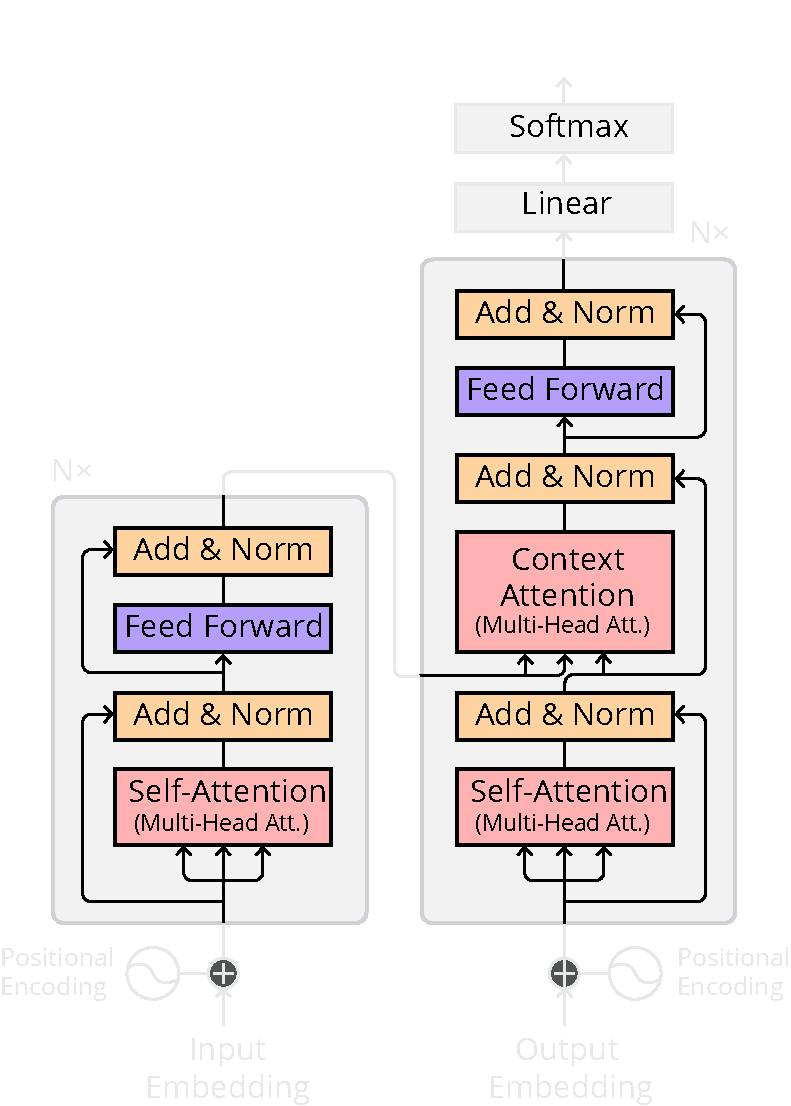
\includegraphics[width=0.9\columnwidth]{figures/transformer_mybg}
%                 \tikz[baseline,remember picture]{\node[anchor=base] (t1){};}
%             \end{center}
%         \end{column}
%     \end{columns}

%     \begin{tikzpicture}[remember picture,overlay]   %% use here too
%         \uncover<2>{\path[draw=tPeony,ultra thick,->](
%             [xshift=2mm,yshift=1mm]n1.north) to [out=6cm,in=0,distance=-1.5cm] ([xshift=-5.13cm,yshift=2.0cm]t1.north);}
%         \uncover<3>{\path[draw=tPeony,ultra thick,->](
%             [xshift=2mm,yshift=1mm]n2.north) to [out=6cm,in=0,distance=-3cm] ([xshift=-2.67cm,yshift=2.0cm]t1.north);}
%         \uncover<4>{\path[draw=tPeony,ultra thick,->](
%             [xshift=2mm,yshift=1mm]n3.north) to [out=-6cm,in=0,distance=-2.5cm] ([xshift=-2.67cm,yshift=3.55cm]t1.north);}
%     \end{tikzpicture}
% \end{frame}

% \begin{frame}
%     \frametitle{Learning $\alpha$}

%     \begin{itemize}
%         \uncover<2->{\item[] {\color{myDarkYellow} Key contribution}: \\\bigskip\quad a closed-form expression for $\pfrac{\aentmax(\x)}{\alpha}$ \quad\emoji{oface}}
%     \end{itemize}

%     \bigskip

%     \begin{itemize}

%         \uncover<3->{\item[] Not trivial! Requires implicit differentiation}

%     \end{itemize}

% \end{frame}

% \begin{frame}
%     \frametitle{Trajetórias de esparsidade}

%     \centering\fontsize{10pt}{15}\selectfont\vspace{-0.5cm}
%     \begin{columns}[T]
%     \begin{column}{0.1\textwidth}
%         \centering
%     \end{column}
%     \begin{column}{0.2\textwidth}
%         \centering
%         \begin{itemize}
%         \vspace{2cm}
%         \item[]\uncover<2->{mais esparso\tikz[remember picture]{\node[coordinate] (n1) {};}}
%         \vspace{0.5cm}
%         \item[]\uncover<3->{mais denso\tikz[remember picture]{\node[coordinate] (n2) {};}}
%         \end{itemize}
%     \end{column}
%     \begin{column}{0.9\textwidth}
%         \centering
%         \vspace{0.5cm}
%         % This file was created by tikzplotlib v0.8.5.
\begin{tikzpicture}

    \definecolor{color0}{rgb}{0.12156862745098,0.466666666666667,0.705882352941177}
    \definecolor{color1}{rgb}{1,0.498039215686275,0.0549019607843137}
    \definecolor{color2}{rgb}{0.172549019607843,0.627450980392157,0.172549019607843}
    \definecolor{color3}{rgb}{0.83921568627451,0.152941176470588,0.156862745098039}
    \definecolor{color4}{rgb}{0.580392156862745,0.403921568627451,0.741176470588235}
    
    \begin{axis}[scaled ticks=false, tick label style={/pgf/number format/.cd, 1000 sep={}},
    legend cell align={left},
    legend style={
        nodes={scale=0.5, transform shape}, at={(0.97,0.42)}, anchor=east, draw=white!80.0!black, fill=myfg!30!mybg, fill opacity=0.6, draw opacity=1,text opacity=1},
    tick align=outside,
    tick pos=left,
    x grid style={white!69.01960784313725!black},
    xlabel={training steps},
    xmin=-500, xmax=13000,
    xtick style={color=white},
    xtick = {0, 4000, 8000, 12000},
    y grid style={white!69.01960784313725!black},
    ylabel={\(\displaystyle \alpha\)},
    ymin=1, ymax=2,
    ytick style={color=white},
    ytick = {1, 1.2, 1.4, 1.6, 1.8, 2},
    width=0.4\columnwidth,
    height=0.4\columnwidth,
    ]
    \addplot [thick, color0, mark=square*, mark size=2, mark repeat=79, mark options={solid}]
    table {%
    18 1.75773811340332
    42 1.75475645065308
    45 1.75405716896057
    56 1.75045299530029
    71 1.74420773983002
    74 1.74278807640076
    94 1.73164820671082
    155 1.68507671356201
    158 1.68310630321503
    167 1.67679250240326
    183 1.66621112823486
    229 1.63320100307465
    234 1.6298725605011
    255 1.61603236198425
    260 1.61318731307983
    267 1.60929274559021
    273 1.6062273979187
    308 1.58366131782532
    310 1.58311796188354
    318 1.57823503017426
    347 1.55986726284027
    367 1.54627776145935
    421 1.52769696712494
    422 1.52798175811768
    442 1.52398872375488
    445 1.52280700206757
    460 1.5197422504425
    463 1.52157425880432
    464 1.52143597602844
    474 1.51942110061646
    536 1.51777052879333
    563 1.51398956775665
    579 1.51327121257782
    586 1.51324605941772
    587 1.51292562484741
    620 1.51289629936218
    634 1.51253867149353
    642 1.51079404354095
    644 1.51114821434021
    647 1.51113629341125
    649 1.51046299934387
    661 1.51197350025177
    671 1.51648259162903
    714 1.52023935317993
    722 1.5212140083313
    730 1.52261590957642
    752 1.52533578872681
    756 1.52611947059631
    765 1.52637791633606
    769 1.52743911743164
    771 1.52748084068298
    785 1.526815533638
    787 1.52683222293854
    792 1.52810597419739
    794 1.52804040908813
    802 1.5276095867157
    808 1.52985072135925
    809 1.52959489822388
    836 1.52904915809631
    907 1.53566002845764
    909 1.53472948074341
    942 1.53326725959778
    945 1.53323030471802
    962 1.53055381774902
    971 1.53268671035767
    972 1.53277540206909
    978 1.53345632553101
    979 1.53339147567749
    984 1.53358376026154
    1002 1.53343534469604
    1005 1.53353548049927
    1014 1.53415584564209
    1063 1.5385320186615
    1066 1.53876638412476
    1072 1.538978099823
    1078 1.5392951965332
    1083 1.5385479927063
    1093 1.53822612762451
    1099 1.53828132152557
    1104 1.53869342803955
    1156 1.54215776920319
    1161 1.5428558588028
    1162 1.54346084594727
    1180 1.54355645179749
    1193 1.54493689537048
    1206 1.54443383216858
    1244 1.54738461971283
    1261 1.55054497718811
    1281 1.55056405067444
    1287 1.55181086063385
    1294 1.55094540119171
    1316 1.55110597610474
    1319 1.55094408988953
    1330 1.55039834976196
    1333 1.55042195320129
    1336 1.54961502552032
    1337 1.54940271377563
    1385 1.55164313316345
    1391 1.55137777328491
    1392 1.5512273311615
    1414 1.55314290523529
    1426 1.55215764045715
    1436 1.5542688369751
    1466 1.55891740322113
    1477 1.55938529968262
    1485 1.55892109870911
    1491 1.56014025211334
    1523 1.56266355514526
    1527 1.56258106231689
    1552 1.56140470504761
    1568 1.56055223941803
    1569 1.5604407787323
    1584 1.56001949310303
    1588 1.5603301525116
    1605 1.5600802898407
    1640 1.56153678894043
    1648 1.56270265579224
    1668 1.56215167045593
    1682 1.56235539913177
    1691 1.56215405464172
    1697 1.5633556842804
    1699 1.56386506557465
    1702 1.56412649154663
    1709 1.56454157829285
    1718 1.56512689590454
    1732 1.56461691856384
    1734 1.56495070457458
    1737 1.56488347053528
    1745 1.56554925441742
    1746 1.56568014621735
    1766 1.56531465053558
    1775 1.56653428077698
    1781 1.56702947616577
    1789 1.5680605173111
    1798 1.56833112239838
    1805 1.56818497180939
    1826 1.57118678092957
    1840 1.57262670993805
    1844 1.57181584835052
    1853 1.5718240737915
    1866 1.57309889793396
    1869 1.57323813438416
    1875 1.57491898536682
    1877 1.57477021217346
    1917 1.57536911964417
    1934 1.57588970661163
    1944 1.57480382919312
    1947 1.57473516464233
    1967 1.57442808151245
    1981 1.57367086410522
    1983 1.57374858856201
    2001 1.57408142089844
    2005 1.57342612743378
    2013 1.57429027557373
    2030 1.57561898231506
    2036 1.57544112205505
    2060 1.5747994184494
    2073 1.57485270500183
    2076 1.57507872581482
    2077 1.57474732398987
    2085 1.57518017292023
    2089 1.57539188861847
    2096 1.57520055770874
    2111 1.57334661483765
    2145 1.57375049591064
    2149 1.57406795024872
    2156 1.57441592216492
    2165 1.57421588897705
    2187 1.57477974891663
    2191 1.57508742809296
    2199 1.5759699344635
    2207 1.57770752906799
    2211 1.57876777648926
    2231 1.58023071289062
    2236 1.5800564289093
    2237 1.57971560955048
    2239 1.57997107505798
    2242 1.58022141456604
    2254 1.5813992023468
    2257 1.58217918872833
    2262 1.58216834068298
    2281 1.58181643486023
    2291 1.58131325244904
    2297 1.58140516281128
    2303 1.58104765415192
    2307 1.58098030090332
    2319 1.58190333843231
    2345 1.58304619789124
    2354 1.58234679698944
    2389 1.58425617218018
    2390 1.58418869972229
    2392 1.58353567123413
    2436 1.58440804481506
    2444 1.58459830284119
    2453 1.58473682403564
    2455 1.58432364463806
    2460 1.58441686630249
    2485 1.58465242385864
    2486 1.58471488952637
    2496 1.58448576927185
    2498 1.58456325531006
    2503 1.58623695373535
    2517 1.58676075935364
    2523 1.58699941635132
    2532 1.58723902702332
    2547 1.58750343322754
    2551 1.58745265007019
    2553 1.58750021457672
    2578 1.58971738815308
    2600 1.59306931495667
    2606 1.59294009208679
    2623 1.59439086914062
    2629 1.59497201442719
    2655 1.59744167327881
    2678 1.59659016132355
    2685 1.59593367576599
    2690 1.59525394439697
    2703 1.59396386146545
    2710 1.59377312660217
    2725 1.59365141391754
    2737 1.5933450460434
    2740 1.59346091747284
    2754 1.59303736686707
    2789 1.59362626075745
    2790 1.59336996078491
    2791 1.59307146072388
    2824 1.59212112426758
    2872 1.59234833717346
    2881 1.59198403358459
    2890 1.5929434299469
    2896 1.59301841259003
    2917 1.59387564659119
    2920 1.59457182884216
    2967 1.59505498409271
    2975 1.59585881233215
    2998 1.59798812866211
    3011 1.59830617904663
    3027 1.60052442550659
    3030 1.6009726524353
    3038 1.60105907917023
    3041 1.60144996643066
    3065 1.60052680969238
    3069 1.60052132606506
    3099 1.59940695762634
    3122 1.59927749633789
    3137 1.59913396835327
    3155 1.59897089004517
    3161 1.59938049316406
    3177 1.60004329681396
    3195 1.599369764328
    3196 1.59925079345703
    3230 1.60110318660736
    3240 1.60094809532166
    3243 1.60130190849304
    3244 1.60102498531342
    3246 1.60116565227509
    3247 1.60114622116089
    3272 1.60180377960205
    3305 1.60286903381348
    3328 1.60269737243652
    3345 1.60305988788605
    3376 1.60560369491577
    3403 1.60580086708069
    3408 1.60572326183319
    3430 1.60704183578491
    3449 1.60619354248047
    3451 1.60620069503784
    3458 1.60603559017181
    3464 1.60527753829956
    3480 1.60496366024017
    3497 1.60441029071808
    3509 1.60530543327332
    3512 1.60491967201233
    3537 1.60392117500305
    3543 1.60464406013489
    3563 1.60380482673645
    3580 1.60340189933777
    3600 1.60352921485901
    3618 1.6047739982605
    3620 1.60489916801453
    3622 1.60521900653839
    3628 1.60558581352234
    3656 1.60612440109253
    3670 1.60642504692078
    3726 1.60476040840149
    3730 1.60566163063049
    3738 1.60669279098511
    3741 1.60685515403748
    3772 1.60784113407135
    3780 1.6081166267395
    3793 1.60778892040253
    3798 1.60868072509766
    3814 1.60893535614014
    3819 1.60909724235535
    3821 1.60901188850403
    3831 1.6089026927948
    3835 1.60892415046692
    3864 1.60875475406647
    3869 1.60800981521606
    3876 1.60877752304077
    3928 1.60910773277283
    3935 1.60916233062744
    3939 1.60928583145142
    3950 1.60920333862305
    3956 1.60868883132935
    3962 1.60904955863953
    3984 1.60955953598022
    4000 1.60896992683411
    4009 1.60951328277588
    4010 1.60947215557098
    4022 1.60955047607422
    4033 1.60953104496002
    4036 1.60990405082703
    4093 1.60888862609863
    4098 1.60851311683655
    4099 1.60865235328674
    4109 1.60862016677856
    4182 1.61328840255737
    4193 1.61327123641968
    4194 1.6132447719574
    4196 1.61370658874512
    4201 1.61373400688171
    4202 1.61355519294739
    4227 1.61331653594971
    4232 1.61270260810852
    4235 1.61247742176056
    4243 1.6129869222641
    4263 1.61108803749084
    4266 1.61096799373627
    4267 1.61100661754608
    4282 1.61099696159363
    4298 1.61066079139709
    4304 1.61028647422791
    4308 1.61021602153778
    4317 1.61123466491699
    4319 1.61127352714539
    4332 1.61032247543335
    4343 1.61109280586243
    4369 1.61034858226776
    4378 1.61025190353394
    4393 1.61146116256714
    4400 1.61150813102722
    4406 1.61139333248138
    4410 1.6112802028656
    4430 1.61301565170288
    4433 1.61300706863403
    4475 1.61166453361511
    4492 1.61242580413818
    4509 1.61327481269836
    4510 1.61403131484985
    4530 1.61435353755951
    4533 1.61437821388245
    4542 1.61458849906921
    4553 1.6158230304718
    4578 1.61733937263489
    4581 1.61735343933105
    4592 1.61726772785187
    4595 1.61729693412781
    4597 1.61733794212341
    4599 1.61729669570923
    4628 1.61622154712677
    4656 1.61694073677063
    4664 1.61672282218933
    4668 1.61741828918457
    4676 1.61721062660217
    4687 1.6168417930603
    4713 1.61728000640869
    4718 1.61684322357178
    4734 1.61715340614319
    4750 1.61721467971802
    4758 1.61729061603546
    4767 1.61773955821991
    4776 1.61834394931793
    4787 1.61859476566315
    4788 1.61859202384949
    4794 1.61875283718109
    4800 1.61865174770355
    4802 1.61896753311157
    4805 1.61940908432007
    4840 1.61944425106049
    4852 1.61916184425354
    4871 1.61937165260315
    4894 1.61983895301819
    4914 1.62001812458038
    4938 1.62014138698578
    4954 1.62135910987854
    4962 1.62149024009705
    4971 1.62126004695892
    4974 1.62171101570129
    4976 1.6219494342804
    5027 1.62063753604889
    5030 1.6208952665329
    5050 1.62050127983093
    5052 1.62036824226379
    5053 1.62006306648254
    5060 1.6198114156723
    5078 1.62027108669281
    5106 1.61947894096375
    5126 1.6193642616272
    5128 1.61936664581299
    5134 1.61970996856689
    5160 1.61914014816284
    5165 1.61953556537628
    5182 1.62005233764648
    5200 1.61942577362061
    5208 1.61954760551453
    5239 1.61852502822876
    5266 1.61983776092529
    5289 1.62182855606079
    5318 1.62310755252838
    5329 1.62423515319824
    5345 1.62574231624603
    5359 1.62609124183655
    5360 1.62603783607483
    5380 1.62569308280945
    5420 1.62506246566772
    5442 1.62496948242188
    5447 1.62555134296417
    5484 1.62525749206543
    5491 1.62437438964844
    5495 1.62427878379822
    5501 1.62452673912048
    5507 1.62485074996948
    5515 1.62515795230865
    5517 1.62531125545502
    5549 1.62485241889954
    5573 1.62448930740356
    5585 1.62416887283325
    5587 1.62417888641357
    5593 1.62407898902893
    5605 1.6244580745697
    5630 1.62373089790344
    5658 1.62549412250519
    5660 1.62608540058136
    5664 1.62641406059265
    5679 1.62704455852509
    5720 1.62802362442017
    5723 1.62798190116882
    5741 1.62823820114136
    5759 1.62820315361023
    5776 1.62685322761536
    5779 1.62666487693787
    5784 1.62700772285461
    5789 1.62686288356781
    5807 1.62667798995972
    5808 1.62677001953125
    5825 1.62728977203369
    5828 1.62700343132019
    5862 1.62715232372284
    5864 1.6269758939743
    5871 1.62693524360657
    5898 1.62575674057007
    5907 1.62568211555481
    5928 1.62668800354004
    5952 1.6269268989563
    5957 1.62794840335846
    5963 1.62797677516937
    5990 1.62797546386719
    6010 1.62844109535217
    6015 1.6286062002182
    6030 1.62909114360809
    6035 1.62901771068573
    6060 1.63031315803528
    6078 1.63123619556427
    6082 1.63117051124573
    6087 1.63097131252289
    6103 1.63219547271729
    6105 1.63244795799255
    6121 1.63195109367371
    6123 1.63174819946289
    6129 1.63192999362946
    6131 1.63188433647156
    6133 1.63203454017639
    6145 1.63213181495667
    6149 1.6320321559906
    6172 1.63240027427673
    6181 1.63225042819977
    6184 1.63215732574463
    6200 1.63256168365479
    6211 1.63210153579712
    6213 1.63200986385345
    6219 1.63208448886871
    6232 1.6323401927948
    6250 1.63137674331665
    6289 1.6313533782959
    6312 1.63187122344971
    6316 1.63224148750305
    6317 1.63239121437073
    6324 1.63223731517792
    6341 1.63258600234985
    6352 1.63232660293579
    6363 1.63263440132141
    6370 1.63282823562622
    6376 1.63261914253235
    6400 1.63183045387268
    6455 1.63266599178314
    6459 1.63280081748962
    6472 1.63400304317474
    6487 1.63480317592621
    6495 1.63474822044373
    6496 1.63492572307587
    6500 1.63493943214417
    6510 1.63461291790009
    6520 1.63449168205261
    6521 1.63427495956421
    6522 1.63414835929871
    6530 1.63440048694611
    6550 1.6338574886322
    6574 1.63451087474823
    6581 1.63395285606384
    6584 1.63392066955566
    6603 1.63306450843811
    6616 1.63285064697266
    6621 1.63268733024597
    6657 1.63351678848267
    6666 1.63322472572327
    6668 1.63313364982605
    6672 1.63330817222595
    6678 1.63343286514282
    6681 1.63317847251892
    6688 1.63371586799622
    6696 1.63419842720032
    6699 1.6343035697937
    6711 1.63422918319702
    6738 1.63502156734467
    6742 1.63481020927429
    6753 1.63497138023376
    6764 1.63486993312836
    6776 1.63509559631348
    6832 1.63701725006104
    6846 1.63702583312988
    6854 1.63706016540527
    6868 1.63764464855194
    6869 1.63761854171753
    6895 1.63664364814758
    6909 1.63696932792664
    6934 1.63688993453979
    6963 1.63611578941345
    6966 1.63602924346924
    6992 1.63618171215057
    7010 1.63640451431274
    7014 1.6361882686615
    7039 1.63656723499298
    7046 1.63619542121887
    7065 1.6367723941803
    7091 1.63660764694214
    7106 1.63772571086884
    7114 1.63748216629028
    7115 1.63738942146301
    7137 1.63759791851044
    7141 1.63779044151306
    7155 1.63671410083771
    7167 1.63679671287537
    7175 1.63633012771606
    7189 1.63655614852905
    7195 1.63723254203796
    7204 1.63798570632935
    7213 1.63830184936523
    7215 1.63850820064545
    7216 1.63848495483398
    7235 1.63886332511902
    7238 1.6391077041626
    7247 1.64007377624512
    7284 1.64094150066376
    7300 1.64146173000336
    7311 1.64108157157898
    7329 1.64128637313843
    7339 1.64118504524231
    7340 1.64104247093201
    7346 1.64145112037659
    7353 1.64128363132477
    7358 1.64136683940887
    7359 1.64139604568481
    7382 1.64140367507935
    7386 1.64145684242249
    7401 1.6418764591217
    7431 1.64089155197144
    7440 1.64084792137146
    7443 1.64084875583649
    7450 1.64067673683167
    7460 1.64055562019348
    7461 1.64044451713562
    7463 1.64042115211487
    7468 1.64062225818634
    7478 1.64032351970673
    7502 1.64072906970978
    7511 1.640709400177
    7530 1.63993322849274
    7547 1.63983392715454
    7596 1.64096450805664
    7609 1.64118599891663
    7612 1.6413676738739
    7643 1.64206600189209
    7644 1.6420316696167
    7661 1.64270126819611
    7671 1.64295721054077
    7676 1.64360547065735
    7687 1.64378464221954
    7693 1.64376842975616
    7700 1.64399933815002
    7718 1.64373660087585
    7723 1.64379501342773
    7728 1.6439745426178
    7746 1.64357912540436
    7757 1.64338374137878
    7760 1.64303874969482
    7780 1.6424515247345
    7788 1.64251339435577
    7798 1.64251255989075
    7810 1.64251184463501
    7833 1.64255881309509
    7838 1.64245319366455
    7899 1.64338064193726
    7900 1.64356875419617
    7904 1.64381372928619
    7932 1.64350414276123
    7975 1.64450359344482
    7983 1.64436459541321
    7991 1.64406502246857
    7992 1.64397263526917
    8026 1.64523506164551
    8037 1.64519560337067
    8049 1.64535021781921
    8052 1.64526891708374
    8058 1.64506554603577
    8066 1.64484333992004
    8126 1.64472627639771
    8150 1.64522409439087
    8157 1.64527368545532
    8180 1.64542865753174
    8184 1.64512538909912
    8198 1.64555239677429
    8215 1.64594173431396
    8221 1.64581120014191
    8234 1.64606189727783
    8254 1.64694547653198
    8263 1.64711952209473
    8279 1.64709496498108
    8290 1.64713096618652
    8299 1.64661681652069
    8307 1.64687788486481
    8327 1.64701211452484
    8329 1.64702081680298
    8332 1.64710688591003
    8334 1.64716839790344
    8340 1.64703691005707
    8352 1.64710927009583
    8360 1.64707922935486
    8363 1.64733529090881
    8368 1.64771962165833
    8375 1.64787924289703
    8377 1.64782667160034
    8428 1.64888787269592
    8439 1.64895844459534
    8447 1.64924621582031
    8467 1.64926481246948
    8468 1.64915633201599
    8470 1.64920449256897
    8484 1.64968109130859
    8488 1.64959001541138
    8497 1.64933133125305
    8498 1.6492760181427
    8503 1.64954447746277
    8507 1.64948868751526
    8508 1.64949774742126
    8523 1.64999663829803
    8554 1.64965510368347
    8566 1.65001082420349
    8573 1.64983606338501
    8578 1.64951407909393
    8592 1.64996409416199
    8601 1.64992713928223
    8616 1.6497288942337
    8627 1.64956974983215
    8634 1.6498110294342
    8635 1.64991116523743
    8644 1.65064859390259
    8682 1.6508629322052
    8690 1.65083885192871
    8691 1.65080285072327
    8695 1.65090918540955
    8727 1.65022397041321
    8774 1.65298306941986
    8778 1.65315413475037
    8796 1.65402364730835
    8801 1.65438973903656
    8816 1.65380072593689
    8819 1.65381002426147
    8822 1.6537663936615
    8843 1.65287637710571
    8854 1.65271472930908
    8868 1.65254664421082
    8878 1.65262258052826
    8885 1.65237641334534
    8902 1.65192675590515
    8904 1.65189814567566
    8907 1.6516706943512
    8928 1.6513786315918
    8930 1.65136706829071
    8935 1.65126717090607
    8946 1.65155220031738
    8954 1.65127754211426
    8958 1.65110158920288
    8975 1.6514995098114
    8993 1.65116286277771
    8999 1.6511116027832
    9004 1.65134990215302
    9009 1.65173494815826
    9012 1.65187406539917
    9027 1.65183663368225
    9028 1.65186166763306
    9055 1.65135073661804
    9063 1.65079474449158
    9073 1.65080463886261
    9084 1.65160775184631
    9105 1.65225565433502
    9123 1.65316271781921
    9155 1.65455031394958
    9156 1.6545991897583
    9162 1.65475797653198
    9214 1.6554958820343
    9216 1.65548348426819
    9226 1.65522289276123
    9233 1.65528094768524
    9260 1.65512430667877
    9281 1.65632271766663
    9291 1.65645384788513
    9307 1.65602707862854
    9309 1.65603470802307
    9316 1.65533983707428
    9348 1.65442967414856
    9353 1.65415143966675
    9364 1.65391540527344
    9365 1.6539888381958
    9369 1.65420389175415
    9412 1.65538251399994
    9415 1.65521788597107
    9435 1.65513253211975
    9441 1.65514039993286
    9442 1.65500044822693
    9468 1.65524959564209
    9475 1.65541708469391
    9482 1.65562677383423
    9537 1.65595984458923
    9538 1.65597975254059
    9547 1.65653455257416
    9554 1.65675926208496
    9557 1.6568603515625
    9564 1.65717625617981
    9567 1.65736389160156
    9586 1.65716564655304
    9589 1.65703797340393
    9600 1.65690648555756
    9611 1.65697205066681
    9621 1.65735602378845
    9623 1.65736889839172
    9624 1.65728354454041
    9627 1.65723752975464
    9651 1.65755832195282
    9656 1.65733575820923
    9657 1.65725886821747
    9661 1.65729880332947
    9680 1.65752017498016
    9690 1.65728735923767
    9698 1.65694081783295
    9710 1.65644717216492
    9750 1.65653944015503
    9759 1.65659093856812
    9760 1.65657556056976
    9766 1.65638530254364
    9768 1.65634882450104
    9777 1.6566219329834
    9812 1.65670275688171
    9840 1.65567409992218
    9843 1.65572690963745
    9855 1.655686378479
    9883 1.65653514862061
    9907 1.65601634979248
    9917 1.65650629997253
    9972 1.6571729183197
    9985 1.65692567825317
    9996 1.65704071521759
    10014 1.65766429901123
    10019 1.65754318237305
    10050 1.65792441368103
    10055 1.65783953666687
    10056 1.65762567520142
    10058 1.65756821632385
    10070 1.65817058086395
    10072 1.65829873085022
    10084 1.65792798995972
    10094 1.65798771381378
    10107 1.65790975093842
    10112 1.65741193294525
    10113 1.65739583969116
    10128 1.65728068351746
    10134 1.65784740447998
    10144 1.65823531150818
    10168 1.65883612632751
    10185 1.65910995006561
    10207 1.65937447547913
    10238 1.65928196907043
    10245 1.65877604484558
    10248 1.65909361839294
    10256 1.66000115871429
    10272 1.66060137748718
    10276 1.66103386878967
    10281 1.66080594062805
    10283 1.66074657440186
    10285 1.66076350212097
    10288 1.66089057922363
    10323 1.66115975379944
    10330 1.66112852096558
    10346 1.66121852397919
    10366 1.66063809394836
    10394 1.6600387096405
    10396 1.66000747680664
    10397 1.66009569168091
    10399 1.6601779460907
    10405 1.66023397445679
    10409 1.66029584407806
    10414 1.66035223007202
    10420 1.66063821315765
    10425 1.66055583953857
    10433 1.66012215614319
    10454 1.6607973575592
    10468 1.6605429649353
    10479 1.66063213348389
    10489 1.66065406799316
    10493 1.66065168380737
    10494 1.66063594818115
    10522 1.66047394275665
    10531 1.6609468460083
    10539 1.6611659526825
    10554 1.66079568862915
    10555 1.6608259677887
    10567 1.66147589683533
    10598 1.66186475753784
    10607 1.6616598367691
    10620 1.66080641746521
    10623 1.66043400764465
    10624 1.66047263145447
    10629 1.66036939620972
    10638 1.66035914421082
    10646 1.66085469722748
    10653 1.66203081607819
    10654 1.66213548183441
    10671 1.66311478614807
    10701 1.66361618041992
    10711 1.66361260414124
    10748 1.66412675380707
    10757 1.66325521469116
    10758 1.66312265396118
    10764 1.6630916595459
    10780 1.66305088996887
    10787 1.66300928592682
    10815 1.66357672214508
    10816 1.66364192962646
    10825 1.66342771053314
    10830 1.66348600387573
    10841 1.66308927536011
    10850 1.6627676486969
    10864 1.66279864311218
    10875 1.66260313987732
    10902 1.6627494096756
    10905 1.66279935836792
    10914 1.66282081604004
    10939 1.66301083564758
    10943 1.66337609291077
    10952 1.6634738445282
    10966 1.66319262981415
    10972 1.66315889358521
    10974 1.66302418708801
    11008 1.66242432594299
    11014 1.66256523132324
    11020 1.6629273891449
    11022 1.66309309005737
    11023 1.66309809684753
    11033 1.66386997699738
    11038 1.66426622867584
    11052 1.66474413871765
    11061 1.66462731361389
    11077 1.66473519802094
    11102 1.66635370254517
    11121 1.66646385192871
    11130 1.66610956192017
    11148 1.66528403759003
    11166 1.66573679447174
    11175 1.66554975509644
    11198 1.66549146175385
    11200 1.66557145118713
    11201 1.66548109054565
    11252 1.66481125354767
    11260 1.66489768028259
    11263 1.6647881269455
    11272 1.66509902477264
    11289 1.66516017913818
    11310 1.66574275493622
    11325 1.66630852222443
    11341 1.66618859767914
    11361 1.66583919525146
    11368 1.6658980846405
    11375 1.66590690612793
    11380 1.66614294052124
    11411 1.66609239578247
    11419 1.66627621650696
    11421 1.66643857955933
    11455 1.66697096824646
    11458 1.66678094863892
    11472 1.66718411445618
    11474 1.66721940040588
    11475 1.66736912727356
    11486 1.6677553653717
    11492 1.667600274086
    11520 1.66692566871643
    11523 1.66686379909515
    11524 1.66676366329193
    11530 1.66640830039978
    11532 1.66642928123474
    11549 1.66601085662842
    11557 1.6661376953125
    11566 1.66645812988281
    11581 1.66658806800842
    11597 1.66677188873291
    11636 1.6671302318573
    11648 1.66717898845673
    11650 1.66732096672058
    11660 1.66759490966797
    11671 1.66777050495148
    11678 1.66776442527771
    11685 1.667560338974
    11687 1.66772139072418
    11704 1.66793131828308
    11723 1.66833353042603
    11759 1.66851854324341
    11769 1.6688334941864
    11786 1.66929912567139
    11792 1.66908776760101
    11801 1.66976654529572
    11831 1.67037487030029
    11854 1.67112421989441
    11855 1.67110633850098
    11873 1.67142462730408
    11901 1.67147934436798
    11906 1.67134201526642
    11919 1.67083728313446
    11920 1.67079770565033
    11933 1.67075371742249
    11941 1.67068219184875
    11946 1.67050099372864
    11948 1.67069268226624
    11949 1.67063415050507
    11969 1.67086279392242
    11974 1.67072057723999
    11986 1.67073202133179
    11988 1.67069983482361
    11998 1.67073345184326
    12003 1.67080402374268
    12010 1.67074978351593
    12025 1.67029571533203
    12029 1.67036056518555
    12041 1.67013716697693
    12061 1.66976702213287
    12076 1.67033052444458
    12085 1.67030811309814
    12090 1.67063879966736
    12133 1.6703667640686
    12138 1.67014932632446
    12147 1.66995477676392
    12153 1.67007756233215
    12164 1.66984438896179
    12168 1.66963195800781
    12184 1.6698853969574
    12197 1.67074358463287
    12217 1.67112040519714
    12226 1.67086815834045
    12234 1.67187547683716
    12254 1.67230772972107
    12270 1.67285668849945
    12290 1.67288827896118
    12293 1.67280983924866
    12309 1.67263531684875
    12323 1.67269849777222
    12325 1.67262864112854
    12336 1.67253959178925
    12396 1.6730535030365
    12405 1.67266535758972
    12406 1.67265641689301
    12436 1.67298698425293
    12455 1.67296695709229
    12458 1.67267537117004
    12480 1.67371296882629
    12517 1.67365431785583
    12524 1.6736478805542
    12545 1.67381882667542
    12551 1.67405533790588
    12553 1.67401516437531
    12574 1.67483234405518
    12596 1.67459344863892
    12599 1.67434251308441
    };
    \addlegendentry{decoder, layer 1, head 8}
    \addplot [thick, color1, mark=star, mark size=2, mark repeat=79, mark options={solid}]
    table {%
    18 1.18035972118378
    42 1.18017363548279
    45 1.18013536930084
    56 1.18011140823364
    71 1.18035387992859
    74 1.18033337593079
    94 1.17896151542664
    155 1.16820526123047
    158 1.16805994510651
    167 1.16709363460541
    183 1.16573882102966
    229 1.15953719615936
    234 1.15892279148102
    255 1.15534460544586
    260 1.15473306179047
    267 1.15359568595886
    273 1.15250241756439
    308 1.14249753952026
    310 1.14223313331604
    318 1.14001441001892
    347 1.12937819957733
    367 1.12400257587433
    421 1.10580778121948
    422 1.10552787780762
    442 1.09977865219116
    445 1.09896087646484
    460 1.09537506103516
    463 1.09485757350922
    464 1.09444999694824
    474 1.09267544746399
    536 1.08129048347473
    563 1.07833290100098
    579 1.0766339302063
    586 1.07508313655853
    587 1.07487916946411
    620 1.07273745536804
    634 1.07202482223511
    642 1.07126653194427
    644 1.07118666172028
    647 1.07104349136353
    649 1.07109713554382
    661 1.06973993778229
    671 1.06875514984131
    714 1.06550693511963
    722 1.064000248909
    730 1.06235778331757
    752 1.06120610237122
    756 1.06063258647919
    765 1.05983865261078
    769 1.05967617034912
    771 1.05970478057861
    785 1.05892515182495
    787 1.05867719650269
    792 1.05859243869781
    794 1.05858492851257
    802 1.05803608894348
    808 1.05752015113831
    809 1.05756163597107
    836 1.05682110786438
    907 1.05345630645752
    909 1.05342972278595
    942 1.05393540859222
    945 1.0538147687912
    962 1.05343306064606
    971 1.05232834815979
    972 1.05227982997894
    978 1.05279695987701
    979 1.05288779735565
    984 1.05316424369812
    1002 1.05298030376434
    1005 1.05274426937103
    1014 1.05280351638794
    1063 1.05114364624023
    1066 1.05098271369934
    1072 1.05156672000885
    1078 1.05168521404266
    1083 1.05162489414215
    1093 1.05122303962708
    1099 1.05110204219818
    1104 1.05102610588074
    1156 1.04846274852753
    1161 1.04810237884521
    1162 1.04813814163208
    1180 1.04785490036011
    1193 1.04770040512085
    1206 1.04747581481934
    1244 1.04707396030426
    1261 1.04715728759766
    1281 1.04664278030396
    1287 1.04662227630615
    1294 1.04665327072144
    1316 1.04786765575409
    1319 1.04775261878967
    1330 1.04789328575134
    1333 1.04785168170929
    1336 1.04793310165405
    1337 1.04788243770599
    1385 1.04777193069458
    1391 1.0476598739624
    1392 1.0476371049881
    1414 1.04791522026062
    1426 1.04792869091034
    1436 1.04775190353394
    1466 1.04747998714447
    1477 1.04739928245544
    1485 1.04722321033478
    1491 1.04650497436523
    1523 1.04567790031433
    1527 1.04555010795593
    1552 1.04490864276886
    1568 1.04488849639893
    1569 1.04495060443878
    1584 1.04500472545624
    1588 1.04497361183167
    1605 1.04473829269409
    1640 1.04444324970245
    1648 1.04448664188385
    1668 1.04448890686035
    1682 1.0446629524231
    1691 1.04569494724274
    1697 1.04584503173828
    1699 1.04586601257324
    1702 1.04588317871094
    1709 1.04604768753052
    1718 1.04615139961243
    1732 1.04629456996918
    1734 1.04611361026764
    1737 1.04576790332794
    1745 1.04597997665405
    1746 1.04600644111633
    1766 1.04634392261505
    1775 1.04639673233032
    1781 1.04651010036469
    1789 1.04638350009918
    1798 1.04655075073242
    1805 1.0467289686203
    1826 1.04603719711304
    1840 1.04600155353546
    1844 1.04628229141235
    1853 1.04627406597137
    1866 1.04603397846222
    1869 1.04610288143158
    1875 1.04552388191223
    1877 1.0453770160675
    1917 1.04422950744629
    1934 1.04400825500488
    1944 1.04413449764252
    1947 1.04413390159607
    1967 1.04388916492462
    1981 1.04410088062286
    1983 1.04402732849121
    2001 1.04378426074982
    2005 1.04380393028259
    2013 1.04389321804047
    2030 1.04384648799896
    2036 1.04367554187775
    2060 1.04388046264648
    2073 1.04488849639893
    2076 1.0450611114502
    2077 1.04508090019226
    2085 1.04530191421509
    2089 1.04541170597076
    2096 1.04552185535431
    2111 1.04580807685852
    2145 1.04583668708801
    2149 1.04594707489014
    2156 1.04609489440918
    2165 1.04620015621185
    2187 1.04629528522491
    2191 1.04630768299103
    2199 1.04626798629761
    2207 1.0461813211441
    2211 1.04578387737274
    2231 1.04593408107758
    2236 1.04598164558411
    2237 1.04600882530212
    2239 1.04592049121857
    2242 1.04597580432892
    2254 1.04588520526886
    2257 1.0455664396286
    2262 1.045205950737
    2281 1.04460656642914
    2291 1.04431796073914
    2297 1.04430723190308
    2303 1.04426062107086
    2307 1.04417169094086
    2319 1.04388928413391
    2345 1.04405105113983
    2354 1.04411923885345
    2389 1.04395699501038
    2390 1.04396879673004
    2392 1.0438939332962
    2436 1.04367637634277
    2444 1.04371798038483
    2453 1.04434454441071
    2455 1.04453098773956
    2460 1.04485130310059
    2485 1.04534530639648
    2486 1.04534387588501
    2496 1.04547595977783
    2498 1.04549896717072
    2503 1.04506039619446
    2517 1.0453280210495
    2523 1.04546749591827
    2532 1.04573202133179
    2547 1.04598259925842
    2551 1.04592728614807
    2553 1.04592502117157
    2578 1.04606664180756
    2600 1.04511451721191
    2606 1.04537785053253
    2623 1.04575371742249
    2629 1.04564452171326
    2655 1.04454517364502
    2678 1.04406189918518
    2685 1.04410970211029
    2690 1.04408895969391
    2703 1.04401767253876
    2710 1.04415285587311
    2725 1.04420292377472
    2737 1.04437100887299
    2740 1.04435753822327
    2754 1.0442111492157
    2789 1.04417908191681
    2790 1.04411578178406
    2791 1.04411053657532
    2824 1.04396319389343
    2872 1.04582250118256
    2881 1.04600274562836
    2890 1.0455801486969
    2896 1.04583311080933
    2917 1.04645121097565
    2920 1.0464985370636
    2967 1.04674816131592
    2975 1.04666125774384
    2998 1.04640293121338
    3011 1.04652607440948
    3027 1.04589366912842
    3030 1.04577326774597
    3038 1.0454386472702
    3041 1.04533052444458
    3065 1.04486012458801
    3069 1.04482388496399
    3099 1.04470944404602
    3122 1.04465794563293
    3137 1.04461967945099
    3155 1.04459607601166
    3161 1.04466104507446
    3177 1.04451501369476
    3195 1.04464709758759
    3196 1.04460966587067
    3230 1.04598391056061
    3240 1.04641366004944
    3243 1.04649806022644
    3244 1.04648184776306
    3246 1.04657447338104
    3247 1.04662215709686
    3272 1.04621374607086
    3305 1.04707765579224
    3328 1.04729223251343
    3345 1.04732143878937
    3376 1.04687607288361
    3403 1.04709458351135
    3408 1.04678606987
    3430 1.04601836204529
    3449 1.0456451177597
    3451 1.04557120800018
    3458 1.04546332359314
    3464 1.04532206058502
    3480 1.04523897171021
    3497 1.04512774944305
    3509 1.04526340961456
    3512 1.04523241519928
    3537 1.04501712322235
    3543 1.0450211763382
    3563 1.04499530792236
    3580 1.04497015476227
    3600 1.04532945156097
    3618 1.04648149013519
    3620 1.0466320514679
    3622 1.04669427871704
    3628 1.04686796665192
    3656 1.04669141769409
    3670 1.04693055152893
    3726 1.04795742034912
    3730 1.0479542016983
    3738 1.04800879955292
    3741 1.04803729057312
    3772 1.04766392707825
    3780 1.04763829708099
    3793 1.04713106155396
    3798 1.04686176776886
    3814 1.04624938964844
    3819 1.0461950302124
    3821 1.04618430137634
    3831 1.04603552818298
    3835 1.04595410823822
    3864 1.04585063457489
    3869 1.04583537578583
    3876 1.04588878154755
    3928 1.04571092128754
    3935 1.04565382003784
    3939 1.04562997817993
    3950 1.04551517963409
    3956 1.04553699493408
    3962 1.04556000232697
    3984 1.04587614536285
    4000 1.04692959785461
    4009 1.04716265201569
    4010 1.04721093177795
    4022 1.04756414890289
    4033 1.04775941371918
    4036 1.04754173755646
    4093 1.04801321029663
    4098 1.04811215400696
    4099 1.04808974266052
    4109 1.04823517799377
    4182 1.04710292816162
    4193 1.0467141866684
    4194 1.04665040969849
    4196 1.04652404785156
    4201 1.04645872116089
    4202 1.04643821716309
    4227 1.0460319519043
    4232 1.04596173763275
    4235 1.04597663879395
    4243 1.04598414897919
    4263 1.04596209526062
    4266 1.04603111743927
    4267 1.04601800441742
    4282 1.0459793806076
    4298 1.04595339298248
    4304 1.04596900939941
    4308 1.04600131511688
    4317 1.04593694210052
    4319 1.04596328735352
    4332 1.04591643810272
    4343 1.04588341712952
    4369 1.04651200771332
    4378 1.04715359210968
    4393 1.04763233661652
    4400 1.047816157341
    4406 1.04787075519562
    4410 1.04799211025238
    4430 1.04775536060333
    4433 1.0478321313858
    4475 1.0483158826828
    4492 1.04864966869354
    4509 1.04836285114288
    4510 1.04828834533691
    4530 1.04808449745178
    4533 1.04816746711731
    4542 1.04818892478943
    4553 1.0480729341507
    4578 1.04694831371307
    4581 1.04686772823334
    4592 1.04672563076019
    4595 1.04662024974823
    4597 1.04653573036194
    4599 1.04652416706085
    4628 1.04617393016815
    4656 1.0460239648819
    4664 1.04609525203705
    4668 1.04606854915619
    4676 1.04602479934692
    4687 1.04592752456665
    4713 1.04576051235199
    4718 1.04579162597656
    4734 1.04579389095306
    4750 1.04593944549561
    4758 1.04663288593292
    4767 1.04702568054199
    4776 1.04739511013031
    4787 1.04746282100677
    4788 1.04748737812042
    4794 1.04758179187775
    4800 1.04756164550781
    4802 1.04740583896637
    4805 1.04729533195496
    4840 1.04789316654205
    4852 1.04799365997314
    4871 1.04819226264954
    4894 1.04800188541412
    4914 1.04784965515137
    4938 1.04788792133331
    4954 1.04708421230316
    4962 1.04677724838257
    4971 1.04659247398376
    4974 1.04652309417725
    4976 1.04649579524994
    5027 1.04632127285004
    5030 1.04622554779053
    5050 1.04620659351349
    5052 1.04617464542389
    5053 1.04613542556763
    5060 1.04609739780426
    5078 1.04619693756104
    5106 1.04599499702454
    5126 1.04590845108032
    5128 1.04596161842346
    5134 1.0461790561676
    5160 1.04751491546631
    5165 1.0475869178772
    5182 1.04788208007812
    5200 1.04790353775024
    5208 1.04798436164856
    5239 1.04823553562164
    5266 1.04846358299255
    5289 1.04793202877045
    5318 1.04816997051239
    5329 1.04776537418365
    5345 1.04726219177246
    5359 1.04708111286163
    5360 1.04702365398407
    5380 1.04675853252411
    5420 1.04662013053894
    5442 1.04665541648865
    5447 1.04664814472198
    5484 1.04645502567291
    5491 1.0464631319046
    5495 1.04644298553467
    5501 1.04642415046692
    5507 1.04638779163361
    5515 1.04648077487946
    5517 1.04661154747009
    5549 1.04806196689606
    5573 1.04787600040436
    5585 1.04826605319977
    5587 1.04831695556641
    5593 1.048419713974
    5605 1.04868984222412
    5630 1.04888331890106
    5658 1.04888164997101
    5660 1.04878556728363
    5664 1.04853129386902
    5679 1.04863274097443
    5720 1.04800081253052
    5723 1.04790139198303
    5741 1.04740190505981
    5759 1.04710173606873
    5776 1.04682159423828
    5779 1.0468043088913
    5784 1.04681527614594
    5789 1.0467369556427
    5807 1.04674053192139
    5808 1.04674243927002
    5825 1.04664695262909
    5828 1.04668736457825
    5862 1.04653406143188
    5864 1.04654157161713
    5871 1.04649102687836
    5898 1.04657459259033
    5907 1.04731392860413
    5928 1.04820787906647
    5952 1.04843640327454
    5957 1.04817926883698
    5963 1.04831671714783
    5990 1.0487197637558
    6010 1.04882431030273
    6015 1.04890048503876
    6030 1.04913926124573
    6035 1.04915630817413
    6060 1.04883599281311
    6078 1.04880249500275
    6082 1.04872965812683
    6087 1.04880404472351
    6103 1.04809641838074
    6105 1.04799199104309
    6121 1.04770612716675
    6123 1.04760885238647
    6129 1.0476211309433
    6131 1.04760372638702
    6133 1.04753828048706
    6145 1.04731094837189
    6149 1.04724788665771
    6172 1.04711556434631
    6181 1.04706490039825
    6184 1.0470654964447
    6200 1.0469788312912
    6211 1.04699873924255
    6213 1.04703462123871
    6219 1.04703450202942
    6232 1.04711067676544
    6250 1.04702627658844
    6289 1.04755067825317
    6312 1.04843497276306
    6316 1.04851627349854
    6317 1.04855954647064
    6324 1.0485817193985
    6341 1.04844081401825
    6352 1.04875862598419
    6363 1.04889941215515
    6370 1.04896378517151
    6376 1.04901170730591
    6400 1.04920983314514
    6455 1.04899978637695
    6459 1.04903292655945
    6472 1.04901528358459
    6487 1.04837930202484
    6495 1.04810738563538
    6496 1.04808843135834
    6500 1.0480101108551
    6510 1.04783225059509
    6520 1.04761862754822
    6521 1.04761743545532
    6522 1.04756677150726
    6530 1.04748630523682
    6550 1.0474339723587
    6574 1.04723346233368
    6581 1.04716157913208
    6584 1.04716849327087
    6603 1.04708683490753
    6616 1.0470974445343
    6621 1.04706823825836
    6657 1.04702591896057
    6666 1.04714941978455
    6668 1.04729604721069
    6672 1.04763269424438
    6678 1.04792070388794
    6681 1.04802632331848
    6688 1.04830491542816
    6696 1.04840111732483
    6699 1.04850244522095
    6711 1.0486855506897
    6738 1.04871213436127
    6742 1.04875957965851
    6753 1.04905104637146
    6764 1.04909479618073
    6776 1.04910111427307
    6832 1.04890191555023
    6846 1.04907691478729
    6854 1.04904699325562
    6868 1.04852294921875
    6869 1.04849004745483
    6895 1.04797458648682
    6909 1.04783284664154
    6934 1.04756999015808
    6963 1.04746878147125
    6966 1.04734349250793
    6992 1.04729974269867
    7010 1.04718947410583
    7014 1.04723763465881
    7039 1.04723227024078
    7046 1.04724526405334
    7065 1.04835689067841
    7091 1.04907667636871
    7106 1.0488908290863
    7114 1.04894733428955
    7115 1.04895496368408
    7137 1.04940223693848
    7141 1.04944241046906
    7155 1.04954934120178
    7167 1.04971408843994
    7175 1.04983401298523
    7189 1.04985463619232
    7195 1.04964363574982
    7204 1.04926323890686
    7213 1.04938793182373
    7215 1.0494476556778
    7216 1.04950201511383
    7235 1.04952263832092
    7238 1.04950094223022
    7247 1.04910159111023
    7284 1.04789710044861
    7300 1.04781031608582
    7311 1.04768800735474
    7329 1.04761183261871
    7339 1.0475560426712
    7340 1.04755640029907
    7346 1.04755485057831
    7353 1.04751443862915
    7358 1.04754328727722
    7359 1.04751908779144
    7382 1.04748928546906
    7386 1.04753887653351
    7401 1.04752850532532
    7431 1.04756999015808
    7440 1.04814398288727
    7443 1.04822814464569
    7450 1.04851591587067
    7460 1.04875326156616
    7461 1.04879808425903
    7463 1.04880523681641
    7468 1.04893612861633
    7478 1.04912889003754
    7502 1.04913103580475
    7511 1.0493129491806
    7530 1.0495126247406
    7547 1.04970419406891
    7596 1.04945003986359
    7609 1.04944825172424
    7612 1.04940164089203
    7643 1.04848051071167
    7644 1.04846775531769
    7661 1.04791676998138
    7671 1.04774153232574
    7676 1.04770529270172
    7687 1.04767274856567
    7693 1.04774248600006
    7700 1.04769909381866
    7718 1.04767632484436
    7723 1.04768145084381
    7728 1.04770231246948
    7746 1.04762363433838
    7757 1.04761242866516
    7760 1.0476371049881
    7780 1.04741334915161
    7788 1.04744017124176
    7798 1.04757916927338
    7810 1.04751408100128
    7833 1.04857218265533
    7838 1.0487916469574
    7899 1.04945397377014
    7900 1.04943871498108
    7904 1.04952263832092
    7932 1.04966938495636
    7975 1.04949295520782
    7983 1.04962420463562
    7991 1.04966080188751
    7992 1.0496678352356
    8026 1.04886674880981
    8037 1.04851424694061
    8049 1.04827439785004
    8052 1.04821574687958
    8058 1.04814887046814
    8066 1.04813599586487
    8126 1.04781830310822
    8150 1.0477157831192
    8157 1.0476633310318
    8180 1.0476393699646
    8184 1.04761350154877
    8198 1.04761099815369
    8215 1.04863297939301
    8221 1.04891359806061
    8234 1.04925930500031
    8254 1.04925322532654
    8263 1.04918968677521
    8279 1.04949331283569
    8290 1.04969429969788
    8299 1.04968976974487
    8307 1.04971194267273
    8327 1.05000042915344
    8329 1.05000436306
    8332 1.05003499984741
    8334 1.05004703998566
    8340 1.05003345012665
    8352 1.04949569702148
    8360 1.0496414899826
    8363 1.04968082904816
    8368 1.0497499704361
    8375 1.04979848861694
    8377 1.04977023601532
    8428 1.04845321178436
    8439 1.04822182655334
    8447 1.04815554618835
    8467 1.04805660247803
    8468 1.04801797866821
    8470 1.0479975938797
    8484 1.04792261123657
    8488 1.04800200462341
    8497 1.04793798923492
    8498 1.04791355133057
    8503 1.04783022403717
    8507 1.0477557182312
    8508 1.04774701595306
    8523 1.04778611660004
    8554 1.04778242111206
    8566 1.04774630069733
    8573 1.04766058921814
    8578 1.04769361019135
    8592 1.04847264289856
    8601 1.04885840415955
    8616 1.04928600788116
    8627 1.04936158657074
    8634 1.04951322078705
    8635 1.04942727088928
    8644 1.04920053482056
    8682 1.04977428913116
    8690 1.04985117912292
    8691 1.04986274242401
    8695 1.04985439777374
    8727 1.05012404918671
    8774 1.04962432384491
    8778 1.04943680763245
    8796 1.0487642288208
    8801 1.04866051673889
    8816 1.04836511611938
    8819 1.04828214645386
    8822 1.04822885990143
    8843 1.04796743392944
    8854 1.04785406589508
    8868 1.04778039455414
    8878 1.04769539833069
    8885 1.04770183563232
    8902 1.04768061637878
    8904 1.04769957065582
    8907 1.04762709140778
    8928 1.04763197898865
    8930 1.04763948917389
    8935 1.04769432544708
    8946 1.04760241508484
    8954 1.04751873016357
    8958 1.0474659204483
    8975 1.04814159870148
    8993 1.04880654811859
    8999 1.04894053936005
    9004 1.04901874065399
    9009 1.04910957813263
    9012 1.04915726184845
    9027 1.04880058765411
    9028 1.04885411262512
    9055 1.04952502250671
    9063 1.04957056045532
    9073 1.04971706867218
    9084 1.04980957508087
    9105 1.0499883890152
    9123 1.04957735538483
    9155 1.04959142208099
    9156 1.04957330226898
    9162 1.04931700229645
    9214 1.04816162586212
    9216 1.04813981056213
    9226 1.04801249504089
    9233 1.04805886745453
    9260 1.04793787002563
    9281 1.04785406589508
    9291 1.0478093624115
    9307 1.04785716533661
    9309 1.04785227775574
    9316 1.04786241054535
    9348 1.0477808713913
    9353 1.04800307750702
    9364 1.04859590530396
    9365 1.04864048957825
    9369 1.04881024360657
    9412 1.04924285411835
    9415 1.04937028884888
    9435 1.04957020282745
    9441 1.04966485500336
    9442 1.04965329170227
    9468 1.04972243309021
    9475 1.04989516735077
    9482 1.04992544651031
    9537 1.04971599578857
    9538 1.04972660541534
    9547 1.04945111274719
    9554 1.04918920993805
    9557 1.04915463924408
    9564 1.04894745349884
    9567 1.04889214038849
    9586 1.04855287075043
    9589 1.04851579666138
    9600 1.04837739467621
    9611 1.04822421073914
    9621 1.04827690124512
    9623 1.0482794046402
    9624 1.04829740524292
    9627 1.04822027683258
    9651 1.04809856414795
    9656 1.04812896251678
    9657 1.048135638237
    9661 1.04813098907471
    9680 1.04814112186432
    9690 1.04810214042664
    9698 1.04810738563538
    9710 1.04799842834473
    9750 1.04884326457977
    9759 1.04906487464905
    9760 1.04909896850586
    9766 1.04929327964783
    9768 1.04933345317841
    9777 1.04956650733948
    9812 1.04964399337769
    9840 1.04992640018463
    9843 1.04991376399994
    9855 1.05012357234955
    9883 1.04987835884094
    9907 1.05001890659332
    9917 1.0499073266983
    9972 1.04850506782532
    9985 1.04846453666687
    9996 1.04837214946747
    10014 1.04821979999542
    10019 1.04825687408447
    10050 1.04820084571838
    10055 1.04816257953644
    10056 1.04815852642059
    10058 1.04813253879547
    10070 1.04816317558289
    10072 1.0481812953949
    10084 1.04817247390747
    10094 1.04815101623535
    10107 1.04812598228455
    10112 1.04816222190857
    10113 1.04815256595612
    10128 1.04879450798035
    10134 1.04900729656219
    10144 1.04926812648773
    10168 1.04967272281647
    10185 1.04966235160828
    10207 1.04984140396118
    10238 1.0500283241272
    10245 1.050088763237
    10248 1.05013811588287
    10256 1.05017709732056
    10272 1.04974865913391
    10276 1.0497899055481
    10281 1.04992389678955
    10283 1.0499552488327
    10285 1.0499861240387
    10288 1.05000507831573
    10323 1.04936742782593
    10330 1.04920506477356
    10346 1.04895102977753
    10366 1.04864501953125
    10394 1.04840421676636
    10396 1.04839849472046
    10397 1.04838573932648
    10399 1.04836511611938
    10405 1.04844176769257
    10409 1.04845142364502
    10414 1.0484881401062
    10420 1.04842567443848
    10425 1.04834413528442
    10433 1.0483455657959
    10454 1.04833137989044
    10468 1.04825150966644
    10479 1.04818880558014
    10489 1.04812455177307
    10493 1.04803550243378
    10494 1.0480682849884
    10522 1.04931962490082
    10531 1.04954874515533
    10539 1.04966044425964
    10554 1.04977822303772
    10555 1.04975879192352
    10567 1.04979515075684
    10598 1.05009543895721
    10607 1.05019235610962
    10620 1.05032932758331
    10623 1.05039465427399
    10624 1.05041110515594
    10629 1.05047202110291
    10638 1.05038833618164
    10646 1.05025815963745
    10653 1.04991459846497
    10654 1.04998600482941
    10671 1.05031967163086
    10701 1.04976201057434
    10711 1.04947507381439
    10748 1.04888105392456
    10757 1.04883325099945
    10758 1.04882335662842
    10764 1.0487368106842
    10780 1.04862821102142
    10787 1.04864406585693
    10815 1.0483433008194
    10816 1.04835200309753
    10825 1.04830944538116
    10830 1.04833769798279
    10841 1.04822301864624
    10850 1.04820203781128
    10864 1.04814183712006
    10875 1.04800868034363
    10902 1.04899024963379
    10905 1.04910230636597
    10914 1.0492627620697
    10939 1.0494863986969
    10943 1.04942405223846
    10952 1.0495810508728
    10966 1.04974544048309
    10972 1.04982841014862
    10974 1.04986846446991
    11008 1.05022573471069
    11014 1.05021846294403
    11020 1.05030572414398
    11022 1.05029201507568
    11023 1.05028390884399
    11033 1.04989290237427
    11038 1.04984772205353
    11052 1.05008578300476
    11061 1.05006730556488
    11077 1.04980182647705
    11102 1.04931271076202
    11121 1.04893326759338
    11130 1.04874670505524
    11148 1.04863023757935
    11166 1.04844558238983
    11175 1.04849898815155
    11198 1.04846060276031
    11200 1.04840433597565
    11201 1.04838860034943
    11252 1.04825758934021
    11260 1.04821908473969
    11263 1.04825031757355
    11272 1.0486558675766
    11289 1.0493391752243
    11310 1.04971396923065
    11325 1.04964196681976
    11341 1.04981732368469
    11361 1.04999244213104
    11368 1.05006420612335
    11375 1.05006670951843
    11380 1.05015623569489
    11411 1.0503556728363
    11419 1.04989409446716
    11421 1.0499415397644
    11455 1.0500922203064
    11458 1.05003178119659
    11472 1.04959893226624
    11474 1.04950153827667
    11475 1.04946637153625
    11486 1.0492171049118
    11492 1.04908454418182
    11520 1.04861342906952
    11523 1.04858541488647
    11524 1.04854536056519
    11530 1.04850518703461
    11532 1.04845118522644
    11549 1.04841196537018
    11557 1.04843842983246
    11566 1.04840838909149
    11581 1.04838299751282
    11597 1.04825055599213
    11636 1.04797339439392
    11648 1.04803383350372
    11650 1.04805672168732
    11660 1.04865729808807
    11671 1.04905164241791
    11678 1.04927730560303
    11685 1.04942572116852
    11687 1.04942607879639
    11704 1.0495617389679
    11723 1.04960203170776
    11759 1.04997503757477
    11769 1.0500739812851
    11786 1.05016732215881
    11792 1.05017817020416
    11801 1.04985809326172
    11831 1.04992055892944
    11854 1.04941403865814
    11855 1.04938471317291
    11873 1.04893827438354
    11901 1.04851603507996
    11906 1.04841959476471
    11919 1.04829967021942
    11920 1.04830574989319
    11933 1.04822301864624
    11941 1.04820370674133
    11946 1.04813754558563
    11948 1.04814994335175
    11949 1.04814231395721
    11969 1.04810190200806
    11974 1.0480614900589
    11986 1.04806005954742
    11988 1.04806208610535
    11998 1.04801797866821
    12003 1.04801964759827
    12010 1.04800963401794
    12025 1.04786050319672
    12029 1.04788911342621
    12041 1.04840469360352
    12061 1.04914700984955
    12076 1.04944705963135
    12085 1.04959154129028
    12090 1.04937279224396
    12133 1.04971349239349
    12138 1.04973256587982
    12147 1.04985904693604
    12153 1.04990351200104
    12164 1.0501195192337
    12168 1.05015897750854
    12184 1.04987370967865
    12197 1.04988372325897
    12217 1.04985415935516
    12226 1.0497111082077
    12234 1.0494943857193
    12254 1.04898607730865
    12270 1.04868161678314
    12290 1.04852962493896
    12293 1.04845142364502
    12309 1.04840660095215
    12323 1.04834568500519
    12325 1.04834365844727
    12336 1.04824936389923
    12396 1.04799842834473
    12405 1.04798567295074
    12406 1.04799020290375
    12436 1.04894506931305
    12455 1.04926359653473
    12458 1.04930996894836
    12480 1.04942381381989
    12517 1.04992723464966
    12524 1.05002093315125
    12545 1.05024063587189
    12551 1.05026566982269
    12553 1.05027461051941
    12574 1.04996454715729
    12596 1.05010497570038
    12599 1.05002892017365
    };
    \addlegendentry{encoder, layer 1, head 3}
    \addplot [thick, color2, mark=triangle*, mark size=2, mark repeat=79, mark options={solid,rotate=180}]
    table {%
    18 1.6881628036499
    42 1.68784439563751
    45 1.68774771690369
    56 1.68646097183228
    71 1.68273270130157
    74 1.6818596124649
    94 1.67471385002136
    155 1.68869996070862
    158 1.68934464454651
    167 1.69216585159302
    183 1.6967533826828
    229 1.7048192024231
    234 1.70547223091125
    255 1.70790362358093
    260 1.70822286605835
    267 1.70907461643219
    273 1.70913147926331
    308 1.71249771118164
    310 1.71258223056793
    318 1.71141839027405
    347 1.70397460460663
    367 1.70710146427155
    421 1.71128034591675
    422 1.71092212200165
    442 1.71390151977539
    445 1.71533632278442
    460 1.71932482719421
    463 1.72011637687683
    464 1.71990895271301
    474 1.72159624099731
    536 1.73295331001282
    563 1.73123788833618
    579 1.72891783714294
    586 1.73138952255249
    587 1.73127293586731
    620 1.73310732841492
    634 1.73277509212494
    642 1.73196744918823
    644 1.73373174667358
    647 1.73413515090942
    649 1.73402142524719
    661 1.73396563529968
    671 1.73456215858459
    714 1.73379564285278
    722 1.73538875579834
    730 1.73844420909882
    752 1.74077415466309
    756 1.74216377735138
    765 1.74383616447449
    769 1.74432754516602
    771 1.74518847465515
    785 1.7460116147995
    787 1.74682140350342
    792 1.7481861114502
    794 1.74838364124298
    802 1.74787926673889
    808 1.74900484085083
    809 1.74878144264221
    836 1.75017857551575
    907 1.75387763977051
    909 1.75459611415863
    942 1.75326085090637
    945 1.75302815437317
    962 1.75161349773407
    971 1.75438249111176
    972 1.75446224212646
    978 1.75493240356445
    979 1.75502681732178
    984 1.75493693351746
    1002 1.75475883483887
    1005 1.75396418571472
    1014 1.75380945205688
    1063 1.75560975074768
    1066 1.75600302219391
    1072 1.75565433502197
    1078 1.75623679161072
    1083 1.75635290145874
    1093 1.75750768184662
    1099 1.75775504112244
    1104 1.75786399841309
    1156 1.76245188713074
    1161 1.76283192634583
    1162 1.76292634010315
    1180 1.76384544372559
    1193 1.76545405387878
    1206 1.76703572273254
    1244 1.77045023441315
    1261 1.77070689201355
    1281 1.77299880981445
    1287 1.77386140823364
    1294 1.7746262550354
    1316 1.77514863014221
    1319 1.77500200271606
    1330 1.77504050731659
    1333 1.77524244785309
    1336 1.77517771720886
    1337 1.77508223056793
    1385 1.7768931388855
    1391 1.77657341957092
    1392 1.7765040397644
    1414 1.77653694152832
    1426 1.7755514383316
    1436 1.77612888813019
    1466 1.77742958068848
    1477 1.7775731086731
    1485 1.77673804759979
    1491 1.77750754356384
    1523 1.77920508384705
    1527 1.77936029434204
    1552 1.7808004617691
    1568 1.78315711021423
    1569 1.78317499160767
    1584 1.78416442871094
    1588 1.78409957885742
    1605 1.78547215461731
    1640 1.78818655014038
    1648 1.78929543495178
    1668 1.79150950908661
    1682 1.79188632965088
    1691 1.79163932800293
    1697 1.79151558876038
    1699 1.79153347015381
    1702 1.79155254364014
    1709 1.79176688194275
    1718 1.79117846488953
    1732 1.79079735279083
    1734 1.79103994369507
    1737 1.79107713699341
    1745 1.79110908508301
    1746 1.79119062423706
    1766 1.79199385643005
    1775 1.7919340133667
    1781 1.79172992706299
    1789 1.79119729995728
    1798 1.79124689102173
    1805 1.79197359085083
    1826 1.79563748836517
    1840 1.79638123512268
    1844 1.79610621929169
    1853 1.79611539840698
    1866 1.7950474023819
    1869 1.79486012458801
    1875 1.79510819911957
    1877 1.79526042938232
    1917 1.79777884483337
    1934 1.79905462265015
    1944 1.79963207244873
    1947 1.79959356784821
    1967 1.80123865604401
    1981 1.80199646949768
    1983 1.80187571048737
    2001 1.80272102355957
    2005 1.80320656299591
    2013 1.80374050140381
    2030 1.80424606800079
    2036 1.80524086952209
    2060 1.80628776550293
    2073 1.8060450553894
    2076 1.80597543716431
    2077 1.80602335929871
    2085 1.8059618473053
    2089 1.80599904060364
    2096 1.80562138557434
    2111 1.80615997314453
    2145 1.8053286075592
    2149 1.8055534362793
    2156 1.80597150325775
    2165 1.80580818653107
    2187 1.80588698387146
    2191 1.80623519420624
    2199 1.8060063123703
    2207 1.80614912509918
    2211 1.80626595020294
    2231 1.80699026584625
    2236 1.80661511421204
    2237 1.8066291809082
    2239 1.80646991729736
    2242 1.80674028396606
    2254 1.80742180347443
    2257 1.80741715431213
    2262 1.80794727802277
    2281 1.80856585502625
    2291 1.80844759941101
    2297 1.80893301963806
    2303 1.80931639671326
    2307 1.80982351303101
    2319 1.80992007255554
    2345 1.81209635734558
    2354 1.81266283988953
    2389 1.81404197216034
    2390 1.81395959854126
    2392 1.81380212306976
    2436 1.81484580039978
    2444 1.81548357009888
    2453 1.81498336791992
    2455 1.81521594524384
    2460 1.8148775100708
    2485 1.81475853919983
    2486 1.81482648849487
    2496 1.81434392929077
    2498 1.81441855430603
    2503 1.81485033035278
    2517 1.81569862365723
    2523 1.81577825546265
    2532 1.81632626056671
    2547 1.81619763374329
    2551 1.81631326675415
    2553 1.81620824337006
    2578 1.81714141368866
    2600 1.81890749931335
    2606 1.81930446624756
    2623 1.8200216293335
    2629 1.82035803794861
    2655 1.8212171792984
    2678 1.82188010215759
    2685 1.82187056541443
    2690 1.82200145721436
    2703 1.82347702980042
    2710 1.82376563549042
    2725 1.82427740097046
    2737 1.82474422454834
    2740 1.82498836517334
    2754 1.82521629333496
    2789 1.82694137096405
    2790 1.82691156864166
    2791 1.82699823379517
    2824 1.82726740837097
    2872 1.82736098766327
    2881 1.82831716537476
    2890 1.82855653762817
    2896 1.82829403877258
    2917 1.82821893692017
    2920 1.82803964614868
    2967 1.82695376873016
    2975 1.82702803611755
    2998 1.82752728462219
    3011 1.82731342315674
    3027 1.82830500602722
    3030 1.82848191261292
    3038 1.82890236377716
    3041 1.82881355285645
    3065 1.82951736450195
    3069 1.82950520515442
    3099 1.83047032356262
    3122 1.83151113986969
    3137 1.83251452445984
    3155 1.83295321464539
    3161 1.83259534835815
    3177 1.83280432224274
    3195 1.83340847492218
    3196 1.83353757858276
    3230 1.83391189575195
    3240 1.83433043956757
    3243 1.83425998687744
    3244 1.83426690101624
    3246 1.83438587188721
    3247 1.83449697494507
    3272 1.83454871177673
    3305 1.83496499061584
    3328 1.83505058288574
    3345 1.83434963226318
    3376 1.83492255210876
    3403 1.83522307872772
    3408 1.83554267883301
    3430 1.83667075634003
    3449 1.83717715740204
    3451 1.83706486225128
    3458 1.83695566654205
    3464 1.83702754974365
    3480 1.8375256061554
    3497 1.83752262592316
    3509 1.83766508102417
    3512 1.83753216266632
    3537 1.8384428024292
    3543 1.83859348297119
    3563 1.83892464637756
    3580 1.83990633487701
    3600 1.83970737457275
    3618 1.8396110534668
    3620 1.83954417705536
    3622 1.83972764015198
    3628 1.83979046344757
    3656 1.84000182151794
    3670 1.84012842178345
    3726 1.84050405025482
    3730 1.84079909324646
    3738 1.84100151062012
    3741 1.84096574783325
    3772 1.84168922901154
    3780 1.84205770492554
    3793 1.84296882152557
    3798 1.84284520149231
    3814 1.84349274635315
    3819 1.84379863739014
    3821 1.84401953220367
    3831 1.84435737133026
    3835 1.84464967250824
    3864 1.84603881835938
    3869 1.84626138210297
    3876 1.8464629650116
    3928 1.84843420982361
    3935 1.84886908531189
    3939 1.84897565841675
    3950 1.84927940368652
    3956 1.84904170036316
    3962 1.84917712211609
    3984 1.84946846961975
    4000 1.8497908115387
    4009 1.8497679233551
    4010 1.8498283624649
    4022 1.85035443305969
    4033 1.85071468353271
    4036 1.85091304779053
    4093 1.85090661048889
    4098 1.85129761695862
    4099 1.85114526748657
    4109 1.85091757774353
    4182 1.85116624832153
    4193 1.85178422927856
    4194 1.85177886486053
    4196 1.85193932056427
    4201 1.8520587682724
    4202 1.85209500789642
    4227 1.8521956205368
    4232 1.85220289230347
    4235 1.85244178771973
    4243 1.85272669792175
    4263 1.85313487052917
    4266 1.85346972942352
    4267 1.85352492332458
    4282 1.85341024398804
    4298 1.85416746139526
    4304 1.85413837432861
    4308 1.85426020622253
    4317 1.85460114479065
    4319 1.85475301742554
    4332 1.85504388809204
    4343 1.85502195358276
    4369 1.85496354103088
    4378 1.85503053665161
    4393 1.85529685020447
    4400 1.85553479194641
    4406 1.8558349609375
    4410 1.85591411590576
    4430 1.85694360733032
    4433 1.85679495334625
    4475 1.85639321804047
    4492 1.8565309047699
    4509 1.85597097873688
    4510 1.85603642463684
    4530 1.85584568977356
    4533 1.85593032836914
    4542 1.85563683509827
    4553 1.85607290267944
    4578 1.8557460308075
    4581 1.85579800605774
    4592 1.8559901714325
    4595 1.85595953464508
    4597 1.85603904724121
    4599 1.85614883899689
    4628 1.85782718658447
    4656 1.85881662368774
    4664 1.85898303985596
    4668 1.85883271694183
    4676 1.85893130302429
    4687 1.85954594612122
    4713 1.85942590236664
    4718 1.8592746257782
    4734 1.859743475914
    4750 1.86027085781097
    4758 1.86008644104004
    4767 1.86035966873169
    4776 1.86017394065857
    4787 1.86002969741821
    4788 1.85996842384338
    4794 1.86031627655029
    4800 1.86068451404572
    4802 1.86071872711182
    4805 1.86052644252777
    4840 1.86055302619934
    4852 1.86054348945618
    4871 1.86052441596985
    4894 1.86035788059235
    4914 1.86042451858521
    4938 1.86083769798279
    4954 1.8612676858902
    4962 1.86161994934082
    4971 1.86171102523804
    4974 1.86206161975861
    4976 1.86209940910339
    5027 1.86239552497864
    5030 1.8624382019043
    5050 1.8627450466156
    5052 1.86268508434296
    5053 1.86259412765503
    5060 1.86288189888
    5078 1.86293888092041
    5106 1.86375463008881
    5126 1.86384785175323
    5128 1.86394786834717
    5134 1.86410069465637
    5160 1.86463570594788
    5165 1.86463391780853
    5182 1.86480510234833
    5200 1.8656599521637
    5208 1.86590027809143
    5239 1.86558842658997
    5266 1.8659291267395
    5289 1.86643075942993
    5318 1.86702394485474
    5329 1.86722755432129
    5345 1.86696553230286
    5359 1.86747300624847
    5360 1.86748504638672
    5380 1.8677282333374
    5420 1.86863815784454
    5442 1.86898970603943
    5447 1.86899709701538
    5484 1.86991703510284
    5491 1.87009787559509
    5495 1.87032246589661
    5501 1.87048721313477
    5507 1.87045907974243
    5515 1.87053847312927
    5517 1.87062573432922
    5549 1.87097978591919
    5573 1.87132906913757
    5585 1.8713264465332
    5587 1.87138199806213
    5593 1.87160563468933
    5605 1.87162375450134
    5630 1.87161087989807
    5658 1.87170910835266
    5660 1.87179851531982
    5664 1.87184619903564
    5679 1.87179851531982
    5720 1.8720451593399
    5723 1.87212634086609
    5741 1.87239992618561
    5759 1.87271928787231
    5776 1.8724684715271
    5779 1.8723738193512
    5784 1.87231183052063
    5789 1.87229251861572
    5807 1.87249779701233
    5808 1.87249779701233
    5825 1.87310123443604
    5828 1.87307178974152
    5862 1.87373828887939
    5864 1.8737576007843
    5871 1.87394618988037
    5898 1.87395167350769
    5907 1.87397217750549
    5928 1.87420237064362
    5952 1.87448132038116
    5957 1.87453508377075
    5963 1.87431561946869
    5990 1.87474775314331
    6010 1.87494766712189
    6015 1.8750627040863
    6030 1.87514984607697
    6035 1.87508988380432
    6060 1.87535166740417
    6078 1.87537896633148
    6082 1.87555384635925
    6087 1.87553036212921
    6103 1.87565648555756
    6105 1.87570464611053
    6121 1.87562847137451
    6123 1.87564039230347
    6129 1.8758692741394
    6131 1.8758898973465
    6133 1.87589073181152
    6145 1.87601375579834
    6149 1.8761670589447
    6172 1.87655329704285
    6181 1.87674880027771
    6184 1.87682509422302
    6200 1.87718260288239
    6211 1.87719321250916
    6213 1.87727808952332
    6219 1.87717628479004
    6232 1.87716937065125
    6250 1.87717390060425
    6289 1.87756407260895
    6312 1.87739908695221
    6316 1.87742328643799
    6317 1.87742638587952
    6324 1.87726509571075
    6341 1.87716233730316
    6352 1.87715768814087
    6363 1.87738084793091
    6370 1.87751221656799
    6376 1.87760829925537
    6400 1.87815141677856
    6455 1.87817430496216
    6459 1.87815821170807
    6472 1.87836217880249
    6487 1.87832748889923
    6495 1.87856578826904
    6496 1.87864065170288
    6500 1.87851405143738
    6510 1.87868332862854
    6520 1.87894833087921
    6521 1.8789427280426
    6522 1.87892937660217
    6530 1.87911689281464
    6550 1.87912821769714
    6574 1.87935209274292
    6581 1.87966895103455
    6584 1.87966084480286
    6603 1.8799569606781
    6616 1.88013005256653
    6621 1.88025498390198
    6657 1.8804270029068
    6666 1.880202293396
    6668 1.88030242919922
    6672 1.88025891780853
    6678 1.88020467758179
    6681 1.88020396232605
    6688 1.88021850585938
    6696 1.88036227226257
    6699 1.8803563117981
    6711 1.88052129745483
    6738 1.88082802295685
    6742 1.88084125518799
    6753 1.88115632534027
    6764 1.88111042976379
    6776 1.88114595413208
    6832 1.88176250457764
    6846 1.88189339637756
    6854 1.8820253610611
    6868 1.88263237476349
    6869 1.88266253471375
    6895 1.88293147087097
    6909 1.88315749168396
    6934 1.88328242301941
    6963 1.88394904136658
    6966 1.88408637046814
    6992 1.88382863998413
    7010 1.88381910324097
    7014 1.88377892971039
    7039 1.88356947898865
    7046 1.88358974456787
    7065 1.88335883617401
    7091 1.88358950614929
    7106 1.88369679450989
    7114 1.88378250598907
    7115 1.88379335403442
    7137 1.88403606414795
    7141 1.88410377502441
    7155 1.88415992259979
    7167 1.88410568237305
    7175 1.88421857357025
    7189 1.88421165943146
    7195 1.88433659076691
    7204 1.88458573818207
    7213 1.88452768325806
    7215 1.88459229469299
    7216 1.8845648765564
    7235 1.884526014328
    7238 1.8844918012619
    7247 1.88460779190063
    7284 1.88461875915527
    7300 1.8846755027771
    7311 1.88488388061523
    7329 1.88441205024719
    7339 1.88463973999023
    7340 1.88465654850006
    7346 1.88487315177917
    7353 1.8849276304245
    7358 1.88504457473755
    7359 1.88506388664246
    7382 1.8856680393219
    7386 1.88565170764923
    7401 1.88592445850372
    7431 1.88609457015991
    7440 1.88592410087585
    7443 1.88581252098083
    7450 1.88588833808899
    7460 1.88592505455017
    7461 1.88597667217255
    7463 1.88592112064362
    7468 1.88582921028137
    7478 1.88559508323669
    7502 1.88562679290771
    7511 1.88562142848969
    7530 1.88557076454163
    7547 1.88515758514404
    7596 1.88473987579346
    7609 1.88479113578796
    7612 1.88493227958679
    7643 1.88490533828735
    7644 1.88488793373108
    7661 1.88505029678345
    7671 1.88502049446106
    7676 1.88519048690796
    7687 1.88525056838989
    7693 1.88538432121277
    7700 1.88540363311768
    7718 1.88608622550964
    7723 1.88625001907349
    7728 1.88625824451447
    7746 1.88584971427917
    7757 1.88592898845673
    7760 1.88596844673157
    7780 1.88624215126038
    7788 1.88637685775757
    7798 1.88622713088989
    7810 1.88652062416077
    7833 1.88683640956879
    7838 1.88690066337585
    7899 1.88700580596924
    7900 1.88708806037903
    7904 1.88725638389587
    7932 1.88752615451813
    7975 1.88760423660278
    7983 1.88775968551636
    7991 1.88788318634033
    7992 1.88786375522614
    8026 1.88800477981567
    8037 1.88803505897522
    8049 1.88824892044067
    8052 1.88824546337128
    8058 1.88828837871552
    8066 1.88858246803284
    8126 1.88897395133972
    8150 1.88930726051331
    8157 1.88929712772369
    8180 1.88962507247925
    8184 1.8896369934082
    8198 1.8898913860321
    8215 1.88992488384247
    8221 1.88992857933044
    8234 1.88980579376221
    8254 1.88949871063232
    8263 1.88934671878815
    8279 1.88935899734497
    8290 1.88944685459137
    8299 1.88943457603455
    8307 1.88933444023132
    8327 1.88921070098877
    8329 1.8891818523407
    8332 1.88925421237946
    8334 1.88934898376465
    8340 1.88941884040833
    8352 1.88944041728973
    8360 1.88935840129852
    8363 1.88934278488159
    8368 1.88946127891541
    8375 1.88962888717651
    8377 1.88972115516663
    8428 1.88994479179382
    8439 1.8902382850647
    8447 1.89033842086792
    8467 1.89035487174988
    8468 1.89041578769684
    8470 1.8903648853302
    8484 1.89052259922028
    8488 1.89061534404755
    8497 1.89060020446777
    8498 1.890625
    8503 1.89041376113892
    8507 1.8905074596405
    8508 1.89047193527222
    8523 1.8907059431076
    8554 1.89136624336243
    8566 1.8914920091629
    8573 1.8916939496994
    8578 1.89166986942291
    8592 1.89160442352295
    8601 1.89182782173157
    8616 1.89175593852997
    8627 1.89184355735779
    8634 1.89178502559662
    8635 1.89177894592285
    8644 1.89200615882874
    8682 1.8924880027771
    8690 1.89235997200012
    8691 1.89232575893402
    8695 1.89243698120117
    8727 1.89219093322754
    8774 1.8921229839325
    8778 1.89219450950623
    8796 1.89241743087769
    8801 1.89245891571045
    8816 1.89250159263611
    8819 1.89274525642395
    8822 1.89264249801636
    8843 1.89250040054321
    8854 1.89269423484802
    8868 1.89295303821564
    8878 1.89299583435059
    8885 1.89297306537628
    8902 1.89291179180145
    8904 1.89296126365662
    8907 1.89292526245117
    8928 1.8931577205658
    8930 1.89312875270844
    8935 1.89342260360718
    8946 1.89365375041962
    8954 1.89372444152832
    8958 1.8937304019928
    8975 1.89383721351624
    8993 1.89385199546814
    8999 1.89385271072388
    9004 1.89382421970367
    9009 1.89386487007141
    9012 1.89397835731506
    9027 1.894047498703
    9028 1.89403057098389
    9055 1.8940407037735
    9063 1.89410090446472
    9073 1.89427351951599
    9084 1.89404773712158
    9105 1.89390826225281
    9123 1.89402937889099
    9155 1.89371967315674
    9156 1.89375853538513
    9162 1.89373850822449
    9214 1.89461922645569
    9216 1.89460909366608
    9226 1.89477550983429
    9233 1.89475238323212
    9260 1.89491426944733
    9281 1.89503192901611
    9291 1.89507436752319
    9307 1.89522325992584
    9309 1.89520585536957
    9316 1.89528667926788
    9348 1.89530205726624
    9353 1.89520859718323
    9364 1.89533448219299
    9365 1.8952944278717
    9369 1.89532971382141
    9412 1.89559102058411
    9415 1.895583152771
    9435 1.89570069313049
    9441 1.8957998752594
    9442 1.89588117599487
    9468 1.89614868164062
    9475 1.89626848697662
    9482 1.89631509780884
    9537 1.89640235900879
    9538 1.89637196063995
    9547 1.89639163017273
    9554 1.89641356468201
    9557 1.89659714698792
    9564 1.89666152000427
    9567 1.896688580513
    9586 1.89722752571106
    9589 1.89718508720398
    9600 1.89726662635803
    9611 1.89722585678101
    9621 1.89739727973938
    9623 1.89743947982788
    9624 1.897456407547
    9627 1.89745593070984
    9651 1.89766097068787
    9656 1.89761304855347
    9657 1.89764404296875
    9661 1.89761579036713
    9680 1.89768695831299
    9690 1.89761805534363
    9698 1.89764404296875
    9710 1.89784479141235
    9750 1.89780473709106
    9759 1.89775991439819
    9760 1.89777040481567
    9766 1.89777565002441
    9768 1.89777112007141
    9777 1.89784216880798
    9812 1.89789795875549
    9840 1.89799082279205
    9843 1.89804637432098
    9855 1.89813351631165
    9883 1.8981921672821
    9907 1.89810037612915
    9917 1.89826107025146
    9972 1.89878666400909
    9985 1.8989132642746
    9996 1.89882171154022
    10014 1.89899456501007
    10019 1.89907336235046
    10050 1.89916026592255
    10055 1.89915204048157
    10056 1.89915072917938
    10058 1.89920234680176
    10070 1.89923596382141
    10072 1.89920401573181
    10084 1.8994140625
    10094 1.89935183525085
    10107 1.89950966835022
    10112 1.89942169189453
    10113 1.89939475059509
    10128 1.89947438240051
    10134 1.89953756332397
    10144 1.89968240261078
    10168 1.89977431297302
    10185 1.89976501464844
    10207 1.89985203742981
    10238 1.900141954422
    10245 1.90005588531494
    10248 1.89994442462921
    10256 1.89992427825928
    10272 1.90020072460175
    10276 1.90010190010071
    10281 1.90017104148865
    10283 1.90010762214661
    10285 1.90017831325531
    10288 1.90031218528748
    10323 1.90061664581299
    10330 1.90056371688843
    10346 1.90094590187073
    10366 1.90133380889893
    10394 1.90114378929138
    10396 1.90113544464111
    10397 1.90114212036133
    10399 1.90112566947937
    10405 1.90115737915039
    10409 1.90110611915588
    10414 1.901083111763
    10420 1.90120196342468
    10425 1.90124917030334
    10433 1.9014276266098
    10454 1.90164494514465
    10468 1.90170836448669
    10479 1.90200996398926
    10489 1.90210330486298
    10493 1.90216064453125
    10494 1.90220904350281
    10522 1.90234303474426
    10531 1.90244519710541
    10539 1.9025661945343
    10554 1.90253877639771
    10555 1.90256381034851
    10567 1.90247082710266
    10598 1.90269029140472
    10607 1.90260982513428
    10620 1.90267550945282
    10623 1.90270948410034
    10624 1.90271306037903
    10629 1.90271425247192
    10638 1.90266585350037
    10646 1.90268075466156
    10653 1.90271425247192
    10654 1.90271806716919
    10671 1.90264737606049
    10701 1.90299570560455
    10711 1.90300524234772
    10748 1.90339469909668
    10757 1.90337216854095
    10758 1.90333664417267
    10764 1.90336978435516
    10780 1.90331184864044
    10787 1.90333139896393
    10815 1.90339851379395
    10816 1.90343809127808
    10825 1.90347647666931
    10830 1.90350544452667
    10841 1.90338575839996
    10850 1.9034698009491
    10864 1.90353405475616
    10875 1.90351223945618
    10902 1.90382027626038
    10905 1.90376603603363
    10914 1.90381669998169
    10939 1.90402245521545
    10943 1.90401494503021
    10952 1.90422368049622
    10966 1.90403199195862
    10972 1.90386581420898
    10974 1.90388488769531
    11008 1.90437364578247
    11014 1.90445876121521
    11020 1.90442180633545
    11022 1.90440630912781
    11023 1.90436398983002
    11033 1.9045295715332
    11038 1.90447235107422
    11052 1.90455341339111
    11061 1.90460562705994
    11077 1.90487146377563
    11102 1.90512013435364
    11121 1.90510702133179
    11130 1.90505814552307
    11148 1.90504026412964
    11166 1.9053407907486
    11175 1.90550112724304
    11198 1.90565061569214
    11200 1.90573143959045
    11201 1.90580201148987
    11252 1.90609645843506
    11260 1.90613484382629
    11263 1.90621376037598
    11272 1.90628468990326
    11289 1.90626621246338
    11310 1.90622711181641
    11325 1.90629696846008
    11341 1.90633463859558
    11361 1.90646433830261
    11368 1.90649271011353
    11375 1.90643954277039
    11380 1.90654397010803
    11411 1.90640997886658
    11419 1.90642726421356
    11421 1.90645039081573
    11455 1.90665769577026
    11458 1.90666079521179
    11472 1.9068249464035
    11474 1.9069242477417
    11475 1.90691661834717
    11486 1.90702295303345
    11492 1.90709578990936
    11520 1.907071352005
    11523 1.90711069107056
    11524 1.90716278553009
    11530 1.90727055072784
    11532 1.90726327896118
    11549 1.90729713439941
    11557 1.90717303752899
    11566 1.90711760520935
    11581 1.90715956687927
    11597 1.90734934806824
    11636 1.90748274326324
    11648 1.90768361091614
    11650 1.90767025947571
    11660 1.90776443481445
    11671 1.90767478942871
    11678 1.90760660171509
    11685 1.90771579742432
    11687 1.90775287151337
    11704 1.9076828956604
    11723 1.90766668319702
    11759 1.90757894515991
    11769 1.90767240524292
    11786 1.90793669223785
    11792 1.90791046619415
    11801 1.90793013572693
    11831 1.90830647945404
    11854 1.90833508968353
    11855 1.90836310386658
    11873 1.90852200984955
    11901 1.90855693817139
    11906 1.90853381156921
    11919 1.90869104862213
    11920 1.9087837934494
    11933 1.90895295143127
    11941 1.90907454490662
    11946 1.9091010093689
    11948 1.9091454744339
    11949 1.90920269489288
    11969 1.90922880172729
    11974 1.90932273864746
    11986 1.90921521186829
    11988 1.90923702716827
    11998 1.90918040275574
    12003 1.90932154655457
    12010 1.90925264358521
    12025 1.90935885906219
    12029 1.9093691110611
    12041 1.90915989875793
    12061 1.90911531448364
    12076 1.90926194190979
    12085 1.90920615196228
    12090 1.90937566757202
    12133 1.90959239006042
    12138 1.90974283218384
    12147 1.90973222255707
    12153 1.90984988212585
    12164 1.91002082824707
    12168 1.90998089313507
    12184 1.90983176231384
    12197 1.90988254547119
    12217 1.91005849838257
    12226 1.91002345085144
    12234 1.9101300239563
    12254 1.91035401821136
    12270 1.91043257713318
    12290 1.91052532196045
    12293 1.91056680679321
    12309 1.9105635881424
    12323 1.91077852249146
    12325 1.91083490848541
    12336 1.91082644462585
    12396 1.91110587120056
    12405 1.91126263141632
    12406 1.91127479076385
    12436 1.91159868240356
    12455 1.911656498909
    12458 1.9117157459259
    12480 1.91170716285706
    12517 1.91189420223236
    12524 1.91188716888428
    12545 1.91189622879028
    12551 1.91200494766235
    12553 1.91200017929077
    12574 1.91179513931274
    12596 1.91208171844482
    12599 1.91210079193115
    };
    \addlegendentry{encoder, layer 1, head 4}
    \addplot [thick, color3, mark=*, mark size=2, mark repeat=79, mark options={solid}]
    table {%
    18 1.51662039756775
    42 1.51599025726318
    45 1.51578593254089
    56 1.51456689834595
    71 1.51215600967407
    74 1.51179647445679
    94 1.50820910930634
    155 1.48516941070557
    158 1.48418509960175
    167 1.48020946979523
    183 1.47534370422363
    229 1.46717846393585
    234 1.46664321422577
    255 1.465252161026
    260 1.46513891220093
    267 1.46515500545502
    273 1.46402215957642
    308 1.45847141742706
    310 1.45796418190002
    318 1.4580671787262
    347 1.45328843593597
    367 1.44856262207031
    421 1.41963744163513
    422 1.41917157173157
    442 1.40770077705383
    445 1.40706670284271
    460 1.40012001991272
    463 1.39845538139343
    464 1.39858627319336
    474 1.39651370048523
    536 1.37244486808777
    563 1.3735044002533
    579 1.37728428840637
    586 1.37744235992432
    587 1.37715458869934
    620 1.37654161453247
    634 1.37861156463623
    642 1.38088655471802
    644 1.3813898563385
    647 1.38235378265381
    649 1.38243675231934
    661 1.3863011598587
    671 1.38758993148804
    714 1.38887786865234
    722 1.38624656200409
    730 1.38554465770721
    752 1.37868440151215
    756 1.37924289703369
    765 1.37784516811371
    769 1.37682557106018
    771 1.37651467323303
    785 1.37332594394684
    787 1.37298667430878
    792 1.37267208099365
    794 1.37224328517914
    802 1.36850297451019
    808 1.36734879016876
    809 1.36633634567261
    836 1.3613189458847
    907 1.35321629047394
    909 1.35315787792206
    942 1.35756659507751
    945 1.35841226577759
    962 1.36205923557281
    971 1.36299324035645
    972 1.36301469802856
    978 1.36301040649414
    979 1.3628945350647
    984 1.36556887626648
    1002 1.3689204454422
    1005 1.36988019943237
    1014 1.37323892116547
    1063 1.38304162025452
    1066 1.38295769691467
    1072 1.38277864456177
    1078 1.38369166851044
    1083 1.38476777076721
    1093 1.38902986049652
    1099 1.38994920253754
    1104 1.39101099967957
    1156 1.38740229606628
    1161 1.38664710521698
    1162 1.38670492172241
    1180 1.38776481151581
    1193 1.38827633857727
    1206 1.3863445520401
    1244 1.38694036006927
    1261 1.38761651515961
    1281 1.38767540454865
    1287 1.38730263710022
    1294 1.38692009449005
    1316 1.38752889633179
    1319 1.38803541660309
    1330 1.39048957824707
    1333 1.39168119430542
    1336 1.39238035678864
    1337 1.39266073703766
    1385 1.40250945091248
    1391 1.40345883369446
    1392 1.40358912944794
    1414 1.40885257720947
    1426 1.41250002384186
    1436 1.41514194011688
    1466 1.41983318328857
    1477 1.42269086837769
    1485 1.42563986778259
    1491 1.42703652381897
    1523 1.4257984161377
    1527 1.42614960670471
    1552 1.42897665500641
    1568 1.42838501930237
    1569 1.42837166786194
    1584 1.42870354652405
    1588 1.42898046970367
    1605 1.43119382858276
    1640 1.43038630485535
    1648 1.4300012588501
    1668 1.42773675918579
    1682 1.42751812934875
    1691 1.42854011058807
    1697 1.42961859703064
    1699 1.42976546287537
    1702 1.42994368076324
    1709 1.43055534362793
    1718 1.43214893341064
    1732 1.43694686889648
    1734 1.43750834465027
    1737 1.43787264823914
    1745 1.43856120109558
    1746 1.43844628334045
    1766 1.44176709651947
    1775 1.44449400901794
    1781 1.44722163677216
    1789 1.44818878173828
    1798 1.45073866844177
    1805 1.45275068283081
    1826 1.45775628089905
    1840 1.45861601829529
    1844 1.45956242084503
    1853 1.46211540699005
    1866 1.46607387065887
    1869 1.46625638008118
    1875 1.46784234046936
    1877 1.46816921234131
    1917 1.469975233078
    1934 1.47163498401642
    1944 1.47036254405975
    1947 1.47043597698212
    1967 1.47261738777161
    1981 1.47311437129974
    1983 1.47317004203796
    2001 1.47198951244354
    2005 1.47201919555664
    2013 1.47222685813904
    2030 1.47304248809814
    2036 1.47247457504272
    2060 1.47370684146881
    2073 1.47423577308655
    2076 1.47489905357361
    2077 1.4750657081604
    2085 1.47662830352783
    2089 1.47708570957184
    2096 1.47836709022522
    2111 1.48221933841705
    2145 1.49139833450317
    2149 1.49229395389557
    2156 1.49465560913086
    2165 1.49601686000824
    2187 1.5000547170639
    2191 1.50066304206848
    2199 1.50340008735657
    2207 1.50528728961945
    2211 1.50603127479553
    2231 1.50955307483673
    2236 1.51072084903717
    2237 1.51115560531616
    2239 1.51183605194092
    2242 1.51177334785461
    2254 1.51487565040588
    2257 1.51576864719391
    2262 1.51617658138275
    2281 1.51732110977173
    2291 1.51881003379822
    2297 1.51986825466156
    2303 1.52009391784668
    2307 1.52080953121185
    2319 1.52120590209961
    2345 1.52271842956543
    2354 1.52206790447235
    2389 1.5211546421051
    2390 1.52113115787506
    2392 1.52095484733582
    2436 1.52328777313232
    2444 1.52302241325378
    2453 1.52253222465515
    2455 1.52271509170532
    2460 1.5229184627533
    2485 1.52638947963715
    2486 1.52630615234375
    2496 1.52812492847443
    2498 1.52891707420349
    2503 1.52810907363892
    2517 1.52898192405701
    2523 1.52980089187622
    2532 1.5311496257782
    2547 1.53326046466827
    2551 1.53379011154175
    2553 1.53418898582458
    2578 1.53937029838562
    2600 1.54145550727844
    2606 1.5420755147934
    2623 1.54491090774536
    2629 1.54541826248169
    2655 1.54680621623993
    2678 1.54817008972168
    2685 1.54764986038208
    2690 1.54708743095398
    2703 1.54781520366669
    2710 1.547771692276
    2725 1.54900860786438
    2737 1.54941415786743
    2740 1.54924285411835
    2754 1.54977607727051
    2789 1.55080604553223
    2790 1.55099701881409
    2791 1.55122971534729
    2824 1.55397129058838
    2872 1.55924022197723
    2881 1.56090974807739
    2890 1.5619695186615
    2896 1.56202816963196
    2917 1.56591796875
    2920 1.56690812110901
    2967 1.57246780395508
    2975 1.57471108436584
    2998 1.57901310920715
    3011 1.58205509185791
    3027 1.5844509601593
    3030 1.58479654788971
    3038 1.58544278144836
    3041 1.58506345748901
    3065 1.58576631546021
    3069 1.58602666854858
    3099 1.58709347248077
    3122 1.58733034133911
    3137 1.5873749256134
    3155 1.5883994102478
    3161 1.58824443817139
    3177 1.58935117721558
    3195 1.58825850486755
    3196 1.58847689628601
    3230 1.59015774726868
    3240 1.59182691574097
    3243 1.59243083000183
    3244 1.59290993213654
    3246 1.5931191444397
    3247 1.59314656257629
    3272 1.5961674451828
    3305 1.59889435768127
    3328 1.60268211364746
    3345 1.60690379142761
    3376 1.61052799224854
    3403 1.6143102645874
    3408 1.61563205718994
    3430 1.61790609359741
    3449 1.61797261238098
    3451 1.61767053604126
    3458 1.61819541454315
    3464 1.61823034286499
    3480 1.62060523033142
    3497 1.62131118774414
    3509 1.62174487113953
    3512 1.6217588186264
    3537 1.62174987792969
    3543 1.62239944934845
    3563 1.62411546707153
    3580 1.62502336502075
    3600 1.62662529945374
    3618 1.62760174274445
    3620 1.62815058231354
    3622 1.62847316265106
    3628 1.62932848930359
    3656 1.63298499584198
    3670 1.63412046432495
    3726 1.64030861854553
    3730 1.64070093631744
    3738 1.64143967628479
    3741 1.64186644554138
    3772 1.64346599578857
    3780 1.64388990402222
    3793 1.64409327507019
    3798 1.64467144012451
    3814 1.64555168151855
    3819 1.64578831195831
    3821 1.64575839042664
    3831 1.64488661289215
    3835 1.64474022388458
    3864 1.6445723772049
    3869 1.6447297334671
    3876 1.64502048492432
    3928 1.64583420753479
    3935 1.64589011669159
    3939 1.64566683769226
    3950 1.64632642269135
    3956 1.6460280418396
    3962 1.64530277252197
    3984 1.6453583240509
    4000 1.64573740959167
    4009 1.64612364768982
    4010 1.64633643627167
    4022 1.64817631244659
    4033 1.64857816696167
    4036 1.64889717102051
    4093 1.65527677536011
    4098 1.6555107831955
    4099 1.6555073261261
    4109 1.65637946128845
    4182 1.66357374191284
    4193 1.66350984573364
    4194 1.66358721256256
    4196 1.66364359855652
    4201 1.6634396314621
    4202 1.66348624229431
    4227 1.66475605964661
    4232 1.66549515724182
    4235 1.66589856147766
    4243 1.6664834022522
    4263 1.666348695755
    4266 1.66575574874878
    4267 1.66571533679962
    4282 1.66593098640442
    4298 1.66534948348999
    4304 1.66552495956421
    4308 1.66575050354004
    4317 1.66571640968323
    4319 1.66571152210236
    4332 1.66586565971375
    4343 1.66585254669189
    4369 1.66644430160522
    4378 1.66734337806702
    4393 1.66878747940063
    4400 1.66911971569061
    4406 1.66927564144135
    4410 1.67000341415405
    4430 1.67196202278137
    4433 1.67196416854858
    4475 1.67721700668335
    4492 1.67928266525269
    4509 1.68075704574585
    4510 1.6810268163681
    4530 1.68273162841797
    4533 1.68290829658508
    4542 1.68410563468933
    4553 1.6856027841568
    4578 1.6863260269165
    4581 1.68702113628387
    4592 1.68736255168915
    4595 1.68729066848755
    4597 1.68743288516998
    4599 1.68755197525024
    4628 1.68867087364197
    4656 1.69019937515259
    4664 1.68989300727844
    4668 1.68968236446381
    4676 1.69007647037506
    4687 1.68944525718689
    4713 1.69025897979736
    4718 1.68986809253693
    4734 1.68943977355957
    4750 1.68933022022247
    4758 1.68968558311462
    4767 1.69018602371216
    4776 1.69080352783203
    4787 1.69234776496887
    4788 1.6923143863678
    4794 1.69295001029968
    4800 1.69279658794403
    4802 1.69287538528442
    4805 1.69284212589264
    4840 1.69508528709412
    4852 1.69569087028503
    4871 1.69746589660645
    4894 1.69943976402283
    4914 1.70071053504944
    4938 1.70347833633423
    4954 1.70377087593079
    4962 1.70416378974915
    4971 1.70452904701233
    4974 1.70460152626038
    4976 1.70446252822876
    5027 1.70557487010956
    5030 1.70614838600159
    5050 1.70737528800964
    5052 1.70749115943909
    5053 1.70759916305542
    5060 1.70751643180847
    5078 1.70778584480286
    5106 1.70710384845734
    5126 1.70730566978455
    5128 1.70731985569
    5134 1.70768666267395
    5160 1.70932292938232
    5165 1.70990097522736
    5182 1.71099209785461
    5200 1.71172690391541
    5208 1.71236276626587
    5239 1.71445894241333
    5266 1.716717004776
    5289 1.71863806247711
    5318 1.72224366664886
    5329 1.72297179698944
    5345 1.72290062904358
    5359 1.72292828559875
    5360 1.72295260429382
    5380 1.72353100776672
    5420 1.72478175163269
    5442 1.72635579109192
    5447 1.72645139694214
    5484 1.7276554107666
    5491 1.72797298431396
    5495 1.728102684021
    5501 1.72819864749908
    5507 1.72860062122345
    5515 1.72868669033051
    5517 1.7285875082016
    5549 1.73020553588867
    5573 1.73150312900543
    5585 1.73250710964203
    5587 1.73258519172668
    5593 1.73244416713715
    5605 1.7333447933197
    5630 1.73592686653137
    5658 1.73787951469421
    5660 1.73845458030701
    5664 1.73878979682922
    5679 1.73992705345154
    5720 1.74325227737427
    5723 1.74310123920441
    5741 1.74379873275757
    5759 1.74458909034729
    5776 1.74412608146667
    5779 1.74410617351532
    5784 1.74446356296539
    5789 1.74508666992188
    5807 1.74531722068787
    5808 1.74532961845398
    5825 1.7458416223526
    5828 1.74589085578918
    5862 1.74583101272583
    5864 1.74577856063843
    5871 1.74668109416962
    5898 1.74736046791077
    5907 1.74780201911926
    5928 1.74912583827972
    5952 1.75018930435181
    5957 1.75086414813995
    5963 1.75084543228149
    5990 1.75238502025604
    6010 1.75368881225586
    6015 1.75414824485779
    6030 1.75548410415649
    6035 1.75599765777588
    6060 1.75822472572327
    6078 1.75946450233459
    6082 1.75981056690216
    6087 1.7601420879364
    6103 1.7595888376236
    6105 1.75964546203613
    6121 1.76003015041351
    6123 1.76000571250916
    6129 1.76005125045776
    6131 1.76006031036377
    6133 1.76020121574402
    6145 1.76041507720947
    6149 1.7603714466095
    6172 1.7610559463501
    6181 1.76197957992554
    6184 1.7620108127594
    6200 1.76235282421112
    6211 1.76216745376587
    6213 1.76210260391235
    6219 1.76247262954712
    6232 1.76284956932068
    6250 1.76310384273529
    6289 1.76408529281616
    6312 1.765958070755
    6316 1.76620101928711
    6317 1.76626813411713
    6324 1.76661491394043
    6341 1.76710915565491
    6352 1.76757192611694
    6363 1.76809239387512
    6370 1.76851344108582
    6376 1.76868319511414
    6400 1.77063655853271
    6455 1.77352738380432
    6459 1.77384328842163
    6472 1.77477288246155
    6487 1.77450466156006
    6495 1.77446842193604
    6496 1.77451407909393
    6500 1.77451324462891
    6510 1.77453827857971
    6520 1.77473032474518
    6521 1.77481627464294
    6522 1.77495956420898
    6530 1.77549207210541
    6550 1.77588891983032
    6574 1.77690076828003
    6581 1.77701318264008
    6584 1.77723348140717
    6603 1.77809607982635
    6616 1.77876830101013
    6621 1.77878141403198
    6657 1.77839422225952
    6666 1.77797853946686
    6668 1.77795600891113
    6672 1.77810025215149
    6678 1.77814877033234
    6681 1.77838957309723
    6688 1.77846038341522
    6696 1.778684258461
    6699 1.77877640724182
    6711 1.77902460098267
    6738 1.77955651283264
    6742 1.77978181838989
    6753 1.78004932403564
    6764 1.78051698207855
    6776 1.7814165353775
    6832 1.78539085388184
    6846 1.78632473945618
    6854 1.78664922714233
    6868 1.78654325008392
    6869 1.7865172624588
    6895 1.78742492198944
    6909 1.78780126571655
    6934 1.78783535957336
    6963 1.78851556777954
    6966 1.78851211071014
    6992 1.78902173042297
    7010 1.78899645805359
    7014 1.78913819789886
    7039 1.78853559494019
    7046 1.78870856761932
    7065 1.78907990455627
    7091 1.7902090549469
    7106 1.7912300825119
    7114 1.79171919822693
    7115 1.79177784919739
    7137 1.79341852664948
    7141 1.79345965385437
    7155 1.79361152648926
    7167 1.79401326179504
    7175 1.79451680183411
    7189 1.79533779621124
    7195 1.79551827907562
    7204 1.79550933837891
    7213 1.79565024375916
    7215 1.79572105407715
    7216 1.79567158222198
    7235 1.79705119132996
    7238 1.79706287384033
    7247 1.79714345932007
    7284 1.79725646972656
    7300 1.79748547077179
    7311 1.79714918136597
    7329 1.79719257354736
    7339 1.79742324352264
    7340 1.79740476608276
    7346 1.79759430885315
    7353 1.79792070388794
    7358 1.79815018177032
    7359 1.79820013046265
    7382 1.79813289642334
    7386 1.79821538925171
    7401 1.79818487167358
    7431 1.79909944534302
    7440 1.79939532279968
    7443 1.79956984519958
    7450 1.80009508132935
    7460 1.80042505264282
    7461 1.80041170120239
    7463 1.80030941963196
    7468 1.80081081390381
    7478 1.80096542835236
    7502 1.80150747299194
    7511 1.80206179618835
    7530 1.80301916599274
    7547 1.80433225631714
    7596 1.80652260780334
    7609 1.8075270652771
    7612 1.8079742193222
    7643 1.80999577045441
    7644 1.80999851226807
    7661 1.81014764308929
    7671 1.81017446517944
    7676 1.81048262119293
    7687 1.81083023548126
    7693 1.81083059310913
    7700 1.81093788146973
    7718 1.81128644943237
    7723 1.81136155128479
    7728 1.81147646903992
    7746 1.81242954730988
    7757 1.81232523918152
    7760 1.81238627433777
    7780 1.81294941902161
    7788 1.8130509853363
    7798 1.8131411075592
    7810 1.81339299678802
    7833 1.81330144405365
    7838 1.81333422660828
    7899 1.8150120973587
    7900 1.81500220298767
    7904 1.81531727313995
    7932 1.81612586975098
    7975 1.81797099113464
    7983 1.81821823120117
    7991 1.81852841377258
    7992 1.81853699684143
    8026 1.81882572174072
    8037 1.81918454170227
    8049 1.81989502906799
    8052 1.8200216293335
    8058 1.82030045986176
    8066 1.82025074958801
    8126 1.82123839855194
    8150 1.82171702384949
    8157 1.8219621181488
    8180 1.82192778587341
    8184 1.82194018363953
    8198 1.82226121425629
    8215 1.82237434387207
    8221 1.82251358032227
    8234 1.8227527141571
    8254 1.82321298122406
    8263 1.82410049438477
    8279 1.82475411891937
    8290 1.82521653175354
    8299 1.82590115070343
    8307 1.82638657093048
    8327 1.82650899887085
    8329 1.82667875289917
    8332 1.82688426971436
    8334 1.82699000835419
    8340 1.82729411125183
    8352 1.82806217670441
    8360 1.82818245887756
    8363 1.82834422588348
    8368 1.82869923114777
    8375 1.82902312278748
    8377 1.82917857170105
    8428 1.83005046844482
    8439 1.83014750480652
    8447 1.83030652999878
    8467 1.83085286617279
    8468 1.83080637454987
    8470 1.83095550537109
    8484 1.83136630058289
    8488 1.83145213127136
    8497 1.83160018920898
    8498 1.83167243003845
    8503 1.83157420158386
    8507 1.83155608177185
    8508 1.83160591125488
    8523 1.83174407482147
    8554 1.83238196372986
    8566 1.83273673057556
    8573 1.83292579650879
    8578 1.83283424377441
    8592 1.83303201198578
    8601 1.83319556713104
    8616 1.83399415016174
    8627 1.83444046974182
    8634 1.83465838432312
    8635 1.83470106124878
    8644 1.8352175951004
    8682 1.83648490905762
    8690 1.83686077594757
    8691 1.83692622184753
    8695 1.83713555335999
    8727 1.83853888511658
    8774 1.84033727645874
    8778 1.84062767028809
    8796 1.84085834026337
    8801 1.84098207950592
    8816 1.84118938446045
    8819 1.84123003482819
    8822 1.84130692481995
    8843 1.84207057952881
    8854 1.84204387664795
    8868 1.84246301651001
    8878 1.84268915653229
    8885 1.84276938438416
    8902 1.84323668479919
    8904 1.84324979782104
    8907 1.84321355819702
    8928 1.84350252151489
    8930 1.84350872039795
    8935 1.84353971481323
    8946 1.8438093662262
    8954 1.8438823223114
    8958 1.84399199485779
    8975 1.84403097629547
    8993 1.84463489055634
    8999 1.84492123126984
    9004 1.84517788887024
    9009 1.84532380104065
    9012 1.845370054245
    9027 1.84544253349304
    9028 1.84552955627441
    9055 1.84633564949036
    9063 1.84652507305145
    9073 1.84700965881348
    9084 1.84734535217285
    9105 1.84843444824219
    9123 1.84892249107361
    9155 1.85012674331665
    9156 1.85012912750244
    9162 1.85052263736725
    9214 1.85169768333435
    9216 1.85175919532776
    9226 1.85200357437134
    9233 1.85216426849365
    9260 1.85243773460388
    9281 1.85243999958038
    9291 1.85246813297272
    9307 1.85256779193878
    9309 1.85258054733276
    9316 1.85268199443817
    9348 1.85288691520691
    9353 1.8529304265976
    9364 1.8531231880188
    9365 1.85307788848877
    9369 1.85321009159088
    9412 1.85439729690552
    9415 1.85449516773224
    9435 1.85505902767181
    9441 1.85530471801758
    9442 1.85533356666565
    9468 1.85610842704773
    9475 1.85638809204102
    9482 1.85653018951416
    9537 1.85770678520203
    9538 1.85778903961182
    9547 1.85787534713745
    9554 1.85792374610901
    9557 1.85801005363464
    9564 1.8581360578537
    9567 1.85832595825195
    9586 1.85868799686432
    9589 1.85874152183533
    9600 1.85855150222778
    9611 1.85879445075989
    9621 1.85896944999695
    9623 1.85893082618713
    9624 1.85898447036743
    9627 1.8591091632843
    9651 1.85966777801514
    9656 1.85977697372437
    9657 1.85976982116699
    9661 1.8597913980484
    9680 1.8598780632019
    9690 1.85985445976257
    9698 1.86001431941986
    9710 1.86006915569305
    9750 1.86030793190002
    9759 1.86057472229004
    9760 1.86058866977692
    9766 1.86061644554138
    9768 1.86062383651733
    9777 1.86110556125641
    9812 1.8616898059845
    9840 1.86254274845123
    9843 1.86273574829102
    9855 1.86294686794281
    9883 1.86319732666016
    9907 1.8640524148941
    9917 1.86455988883972
    9972 1.86605513095856
    9985 1.86616969108582
    9996 1.86655592918396
    10014 1.86726629734039
    10019 1.86743116378784
    10050 1.86799299716949
    10055 1.86807250976562
    10056 1.86806273460388
    10058 1.86813771724701
    10070 1.86848700046539
    10072 1.86849820613861
    10084 1.86862087249756
    10094 1.86880373954773
    10107 1.86887097358704
    10112 1.8687219619751
    10113 1.86871004104614
    10128 1.86872220039368
    10134 1.86882591247559
    10144 1.86913621425629
    10168 1.86956214904785
    10185 1.86988997459412
    10207 1.87064683437347
    10238 1.87108945846558
    10245 1.87142086029053
    10248 1.87153029441833
    10256 1.87162280082703
    10272 1.87175989151001
    10276 1.87183117866516
    10281 1.8718341588974
    10283 1.87193882465363
    10285 1.8720451593399
    10288 1.87213122844696
    10323 1.87403035163879
    10330 1.87414789199829
    10346 1.87427568435669
    10366 1.87485027313232
    10394 1.8752533197403
    10396 1.87534260749817
    10397 1.87540364265442
    10399 1.87545168399811
    10405 1.8757758140564
    10409 1.87582969665527
    10414 1.87582170963287
    10420 1.87585115432739
    10425 1.87580251693726
    10433 1.87585461139679
    10454 1.87585306167603
    10468 1.87590885162354
    10479 1.87608480453491
    10489 1.87621212005615
    10493 1.87616455554962
    10494 1.87609148025513
    10522 1.87666034698486
    10531 1.87695455551147
    10539 1.87719118595123
    10554 1.8775269985199
    10555 1.87759470939636
    10567 1.87780165672302
    10598 1.87837481498718
    10607 1.87863683700562
    10620 1.87880206108093
    10623 1.87889444828033
    10624 1.87893283367157
    10629 1.87924575805664
    10638 1.87950682640076
    10646 1.87977850437164
    10653 1.87981772422791
    10654 1.87980222702026
    10671 1.87983107566833
    10701 1.88096225261688
    10711 1.88104391098022
    10748 1.88179397583008
    10757 1.881991147995
    10758 1.88200187683105
    10764 1.88206803798676
    10780 1.88222885131836
    10787 1.88219511508942
    10815 1.8825945854187
    10816 1.88258647918701
    10825 1.88255214691162
    10830 1.88263297080994
    10841 1.88275218009949
    10850 1.8830304145813
    10864 1.88341820240021
    10875 1.88332045078278
    10902 1.88383364677429
    10905 1.88390028476715
    10914 1.8842408657074
    10939 1.88453531265259
    10943 1.88445591926575
    10952 1.88430762290955
    10966 1.88451111316681
    10972 1.88485586643219
    10974 1.88497292995453
    11008 1.88579559326172
    11014 1.88571524620056
    11020 1.88583850860596
    11022 1.88596642017365
    11023 1.88597130775452
    11033 1.88643562793732
    11038 1.88668537139893
    11052 1.88697218894958
    11061 1.88735258579254
    11077 1.88753747940063
    11102 1.88785266876221
    11121 1.88836944103241
    11130 1.88834595680237
    11148 1.88843739032745
    11166 1.88870561122894
    11175 1.88875496387482
    11198 1.8888441324234
    11200 1.88886451721191
    11201 1.88886523246765
    11252 1.88908720016479
    11260 1.88899874687195
    11263 1.88898324966431
    11272 1.8892707824707
    11289 1.88990938663483
    11310 1.890460729599
    11325 1.89053702354431
    11341 1.89063262939453
    11361 1.8913094997406
    11368 1.89145064353943
    11375 1.8917121887207
    11380 1.89177489280701
    11411 1.89251303672791
    11419 1.89286780357361
    11421 1.89291036128998
    11455 1.89362108707428
    11458 1.89368641376495
    11472 1.89367163181305
    11474 1.89366292953491
    11475 1.89370942115784
    11486 1.89369678497314
    11492 1.89358472824097
    11520 1.89393830299377
    11523 1.89387512207031
    11524 1.89389777183533
    11530 1.89396953582764
    11532 1.8939710855484
    11549 1.89440512657166
    11557 1.89456105232239
    11566 1.89473462104797
    11581 1.89488613605499
    11597 1.89537501335144
    11636 1.89537906646729
    11648 1.8954393863678
    11650 1.8954873085022
    11660 1.89556503295898
    11671 1.89584922790527
    11678 1.89592468738556
    11685 1.89590406417847
    11687 1.89591574668884
    11704 1.89598202705383
    11723 1.89628624916077
    11759 1.89693427085876
    11769 1.89711403846741
    11786 1.8976936340332
    11792 1.89782214164734
    11801 1.89832496643066
    11831 1.89886617660522
    11854 1.89952373504639
    11855 1.89954817295074
    11873 1.89974403381348
    11901 1.89996409416199
    11906 1.89994668960571
    11919 1.900141954422
    11920 1.90015363693237
    11933 1.9006233215332
    11941 1.90067720413208
    11946 1.90080118179321
    11948 1.90090155601501
    11949 1.90090751647949
    11969 1.9010956287384
    11974 1.90114176273346
    11986 1.90126132965088
    11988 1.90126049518585
    11998 1.90132069587708
    12003 1.9013397693634
    12010 1.90127515792847
    12025 1.90133285522461
    12029 1.90129029750824
    12041 1.9014892578125
    12061 1.90171837806702
    12076 1.90205585956573
    12085 1.9021418094635
    12090 1.90206980705261
    12133 1.90246975421906
    12138 1.90274012088776
    12147 1.90287280082703
    12153 1.90305018424988
    12164 1.90325081348419
    12168 1.90324854850769
    12184 1.90379667282104
    12197 1.9040162563324
    12217 1.90438914299011
    12226 1.90466713905334
    12234 1.90468561649323
    12254 1.90506339073181
    12270 1.90524184703827
    12290 1.90526723861694
    12293 1.90524780750275
    12309 1.90557074546814
    12323 1.90586566925049
    12325 1.905921459198
    12336 1.90567111968994
    12396 1.90597486495972
    12405 1.90598905086517
    12406 1.9059751033783
    12436 1.9063732624054
    12455 1.9070748090744
    12458 1.90706324577332
    12480 1.90766823291779
    12517 1.90796780586243
    12524 1.90807175636292
    12545 1.908358335495
    12551 1.90854036808014
    12553 1.90858769416809
    12574 1.90893340110779
    12596 1.90912890434265
    12599 1.90929114818573
    };
    \addlegendentry{encoder, layer 2, head 8}
    \addplot [thick, color4, mark=diamond*, mark size=2, mark repeat=79, mark options={solid}]
    table {%
    18 1.9317901134491
    42 1.93166530132294
    45 1.93166291713715
    56 1.93143582344055
    71 1.93086504936218
    74 1.93062305450439
    94 1.92922043800354
    155 1.91884326934814
    158 1.91817164421082
    167 1.91627013683319
    183 1.91284465789795
    229 1.90137839317322
    234 1.89948797225952
    255 1.89224088191986
    260 1.88995897769928
    267 1.88841462135315
    273 1.88659703731537
    308 1.87293887138367
    310 1.87176418304443
    318 1.8679347038269
    347 1.85600590705872
    367 1.84879469871521
    421 1.82904291152954
    422 1.82855558395386
    442 1.82051205635071
    445 1.82007122039795
    460 1.8154000043869
    463 1.81343698501587
    464 1.81344628334045
    474 1.80994510650635
    536 1.77894186973572
    563 1.76262414455414
    579 1.75237834453583
    586 1.74862456321716
    587 1.74845373630524
    620 1.72831392288208
    634 1.71844720840454
    642 1.71365332603455
    644 1.71197021007538
    647 1.71016192436218
    649 1.70865154266357
    661 1.70034050941467
    671 1.69361960887909
    714 1.66118907928467
    722 1.65630984306335
    730 1.65196990966797
    752 1.64202880859375
    756 1.6401481628418
    765 1.63626432418823
    769 1.63523817062378
    771 1.63382470607758
    785 1.62581062316895
    787 1.62467479705811
    792 1.6207309961319
    794 1.61927247047424
    802 1.61352849006653
    808 1.60960078239441
    809 1.60924530029297
    836 1.59317970275879
    907 1.55611717700958
    909 1.55408501625061
    942 1.53170871734619
    945 1.52914595603943
    962 1.51777648925781
    971 1.51166081428528
    972 1.51099848747253
    978 1.50714755058289
    979 1.50645804405212
    984 1.5039222240448
    1002 1.48989057540894
    1005 1.48832714557648
    1014 1.48368978500366
    1063 1.45301616191864
    1066 1.45180320739746
    1072 1.44930636882782
    1078 1.44477343559265
    1083 1.44214808940887
    1093 1.43266534805298
    1099 1.42869508266449
    1104 1.42532825469971
    1156 1.4026951789856
    1161 1.4020060300827
    1162 1.40167808532715
    1180 1.39347767829895
    1193 1.38779544830322
    1206 1.38538336753845
    1244 1.37025380134583
    1261 1.36552488803864
    1281 1.35827398300171
    1287 1.35654711723328
    1294 1.35503232479095
    1316 1.34659218788147
    1319 1.34530878067017
    1330 1.34263253211975
    1333 1.34118008613586
    1336 1.34005868434906
    1337 1.33999621868134
    1385 1.32460355758667
    1391 1.32162594795227
    1392 1.32102346420288
    1414 1.31273984909058
    1426 1.31047677993774
    1436 1.30754566192627
    1466 1.30002224445343
    1477 1.29442286491394
    1485 1.29248881340027
    1491 1.29082584381104
    1523 1.28454160690308
    1527 1.28407037258148
    1552 1.28009748458862
    1568 1.27844500541687
    1569 1.27818584442139
    1584 1.27631664276123
    1588 1.27583885192871
    1605 1.27415883541107
    1640 1.26872074604034
    1648 1.26766085624695
    1668 1.26389670372009
    1682 1.26319074630737
    1691 1.26289987564087
    1697 1.26194393634796
    1699 1.26221823692322
    1702 1.26140034198761
    1709 1.26089406013489
    1718 1.25991320610046
    1732 1.25788414478302
    1734 1.2572637796402
    1737 1.25643718242645
    1745 1.25535345077515
    1746 1.25514554977417
    1766 1.25265264511108
    1775 1.25114154815674
    1781 1.25073647499084
    1789 1.24963068962097
    1798 1.24906241893768
    1805 1.2477912902832
    1826 1.24506938457489
    1840 1.24484646320343
    1844 1.24435245990753
    1853 1.24282038211823
    1866 1.24165606498718
    1869 1.24117612838745
    1875 1.240309715271
    1877 1.24016833305359
    1917 1.23654448986053
    1934 1.23628056049347
    1944 1.23539125919342
    1947 1.23528552055359
    1967 1.23408532142639
    1981 1.23389768600464
    1983 1.23385322093964
    2001 1.23299241065979
    2005 1.23241174221039
    2013 1.23256874084473
    2030 1.23156273365021
    2036 1.23082256317139
    2060 1.23044466972351
    2073 1.23049700260162
    2076 1.23072099685669
    2077 1.23055279254913
    2085 1.22990083694458
    2089 1.22985053062439
    2096 1.22984933853149
    2111 1.22951090335846
    2145 1.2266538143158
    2149 1.22634184360504
    2156 1.22592437267303
    2165 1.22477841377258
    2187 1.22345685958862
    2191 1.22326862812042
    2199 1.22369933128357
    2207 1.22219824790955
    2211 1.2219580411911
    2231 1.22200107574463
    2236 1.22138607501984
    2237 1.22128462791443
    2239 1.2210785150528
    2242 1.22043466567993
    2254 1.21944940090179
    2257 1.21891438961029
    2262 1.21886658668518
    2281 1.21896946430206
    2291 1.218376994133
    2297 1.21829128265381
    2303 1.21834087371826
    2307 1.21810460090637
    2319 1.21732211112976
    2345 1.21622037887573
    2354 1.21603107452393
    2389 1.21548283100128
    2390 1.21558368206024
    2392 1.21551966667175
    2436 1.21473932266235
    2444 1.2146418094635
    2453 1.21555149555206
    2455 1.21588051319122
    2460 1.21607136726379
    2485 1.21578466892242
    2486 1.21585869789124
    2496 1.21626234054565
    2498 1.21602749824524
    2503 1.2156937122345
    2517 1.21517956256866
    2523 1.21462500095367
    2532 1.21471583843231
    2547 1.21409940719604
    2551 1.21388292312622
    2553 1.2137975692749
    2578 1.21410048007965
    2600 1.21375942230225
    2606 1.21428680419922
    2623 1.21348524093628
    2629 1.21296942234039
    2655 1.21285605430603
    2678 1.211470246315
    2685 1.21112966537476
    2690 1.21104526519775
    2703 1.21067714691162
    2710 1.21035349369049
    2725 1.21010315418243
    2737 1.21020495891571
    2740 1.2103556394577
    2754 1.21063435077667
    2789 1.21057379245758
    2790 1.21048879623413
    2791 1.21053540706635
    2824 1.2103328704834
    2872 1.21143341064453
    2881 1.211217045784
    2890 1.21046030521393
    2896 1.21070444583893
    2917 1.20983362197876
    2920 1.20996999740601
    2967 1.20897006988525
    2975 1.20826637744904
    2998 1.20806503295898
    3011 1.20764684677124
    3027 1.20718252658844
    3030 1.20713078975677
    3038 1.20737338066101
    3041 1.20732319355011
    3065 1.20691061019897
    3069 1.20697629451752
    3099 1.20569729804993
    3122 1.20553588867188
    3137 1.20623230934143
    3155 1.20647072792053
    3161 1.2062783241272
    3177 1.20671474933624
    3195 1.20661866664886
    3196 1.20670688152313
    3230 1.20730865001678
    3240 1.20729374885559
    3243 1.20729196071625
    3244 1.20748496055603
    3246 1.20772647857666
    3247 1.20774686336517
    3272 1.20802688598633
    3305 1.20800530910492
    3328 1.20810306072235
    3345 1.20759296417236
    3376 1.20789551734924
    3403 1.20634198188782
    3408 1.20626246929169
    3430 1.2054637670517
    3449 1.20530831813812
    3451 1.20561909675598
    3458 1.2054249048233
    3464 1.20538830757141
    3480 1.20509386062622
    3497 1.20523881912231
    3509 1.20498263835907
    3512 1.20533525943756
    3537 1.20609092712402
    3543 1.20621168613434
    3563 1.20655047893524
    3580 1.20606112480164
    3600 1.20637154579163
    3618 1.20708477497101
    3620 1.20702230930328
    3622 1.20700490474701
    3628 1.20736074447632
    3656 1.20778727531433
    3670 1.20817828178406
    3726 1.20691967010498
    3730 1.20713973045349
    3738 1.20765507221222
    3741 1.20739161968231
    3772 1.20744621753693
    3780 1.20732641220093
    3793 1.20711481571198
    3798 1.20704579353333
    3814 1.20647346973419
    3819 1.2062326669693
    3821 1.20622682571411
    3831 1.20603132247925
    3835 1.20603942871094
    3864 1.20607113838196
    3869 1.20614433288574
    3876 1.20603406429291
    3928 1.20680618286133
    3935 1.20668828487396
    3939 1.20677328109741
    3950 1.20667290687561
    3956 1.20653331279755
    3962 1.20645928382874
    3984 1.20724308490753
    4000 1.20755171775818
    4009 1.2076256275177
    4010 1.20771288871765
    4022 1.20831394195557
    4033 1.20788407325745
    4036 1.20809376239777
    4093 1.20780277252197
    4098 1.20793867111206
    4099 1.20801186561584
    4109 1.20780324935913
    4182 1.20730197429657
    4193 1.20719134807587
    4194 1.20729780197144
    4196 1.20718729496002
    4201 1.20704281330109
    4202 1.20688223838806
    4227 1.20705687999725
    4232 1.20702600479126
    4235 1.20691668987274
    4243 1.20683836936951
    4263 1.20659863948822
    4266 1.20638799667358
    4267 1.20642340183258
    4282 1.20626449584961
    4298 1.20675837993622
    4304 1.20708441734314
    4308 1.20700478553772
    4317 1.20686709880829
    4319 1.20682370662689
    4332 1.20677137374878
    4343 1.20669746398926
    4369 1.20737338066101
    4378 1.20757555961609
    4393 1.20827889442444
    4400 1.20876705646515
    4406 1.20906805992126
    4410 1.20876705646515
    4430 1.20909452438354
    4433 1.20903933048248
    4475 1.20818543434143
    4492 1.20833539962769
    4509 1.20844686031342
    4510 1.20839548110962
    4530 1.20830595493317
    4533 1.20857238769531
    4542 1.20843601226807
    4553 1.20842361450195
    4578 1.20780730247498
    4581 1.20765328407288
    4592 1.20694768428802
    4595 1.20692217350006
    4597 1.20686280727386
    4599 1.20676839351654
    4628 1.20714163780212
    4656 1.20678234100342
    4664 1.20667815208435
    4668 1.20683431625366
    4676 1.20696532726288
    4687 1.20712625980377
    4713 1.20762395858765
    4718 1.20739591121674
    4734 1.20734834671021
    4750 1.20757949352264
    4758 1.20810723304749
    4767 1.2079873085022
    4776 1.20808434486389
    4787 1.20866239070892
    4788 1.20884215831757
    4794 1.20838987827301
    4800 1.20870769023895
    4802 1.20833802223206
    4805 1.2084344625473
    4840 1.20919406414032
    4852 1.20875322818756
    4871 1.20833873748779
    4894 1.20846438407898
    4914 1.20897722244263
    4938 1.20841991901398
    4954 1.20803570747375
    4962 1.20827972888947
    4971 1.2081401348114
    4974 1.20790946483612
    4976 1.2079998254776
    5027 1.20753788948059
    5030 1.20767307281494
    5050 1.20763099193573
    5052 1.20770263671875
    5053 1.20784318447113
    5060 1.2078549861908
    5078 1.20815896987915
    5106 1.20828354358673
    5126 1.20804381370544
    5128 1.20817136764526
    5134 1.20825719833374
    5160 1.20910823345184
    5165 1.20925998687744
    5182 1.20938742160797
    5200 1.20949614048004
    5208 1.20952165126801
    5239 1.20916700363159
    5266 1.20913481712341
    5289 1.20923280715942
    5318 1.20912671089172
    5329 1.20886099338531
    5345 1.20959424972534
    5359 1.2090836763382
    5360 1.20896434783936
    5380 1.20939826965332
    5420 1.2092981338501
    5442 1.20951986312866
    5447 1.20927512645721
    5484 1.21016848087311
    5491 1.21027946472168
    5495 1.2100476026535
    5501 1.20995724201202
    5507 1.21016407012939
    5515 1.21037602424622
    5517 1.21045172214508
    5549 1.21129024028778
    5573 1.21136605739594
    5585 1.21171617507935
    5587 1.21182489395142
    5593 1.21145486831665
    5605 1.21151566505432
    5630 1.2109706401825
    5658 1.21140050888062
    5660 1.21119749546051
    5664 1.21141958236694
    5679 1.21171760559082
    5720 1.21061849594116
    5723 1.21065127849579
    5741 1.21046090126038
    5759 1.21028137207031
    5776 1.21020269393921
    5779 1.21024477481842
    5784 1.21033334732056
    5789 1.21014499664307
    5807 1.21011984348297
    5808 1.21015954017639
    5825 1.21043789386749
    5828 1.21019279956818
    5862 1.21097135543823
    5864 1.21108603477478
    5871 1.2108895778656
    5898 1.21124649047852
    5907 1.21199798583984
    5928 1.21248006820679
    5952 1.21272087097168
    5957 1.21271800994873
    5963 1.21322250366211
    5990 1.21338105201721
    6010 1.21258175373077
    6015 1.21258211135864
    6030 1.21250092983246
    6035 1.21327459812164
    6060 1.21334791183472
    6078 1.21317541599274
    6082 1.21299207210541
    6087 1.21296346187592
    6103 1.21224224567413
    6105 1.21231985092163
    6121 1.21233642101288
    6123 1.21226143836975
    6129 1.21204304695129
    6131 1.21195602416992
    6133 1.21189737319946
    6145 1.21216404438019
    6149 1.21226787567139
    6172 1.21179568767548
    6181 1.21162128448486
    6184 1.21162223815918
    6200 1.21179819107056
    6211 1.21162247657776
    6213 1.21174442768097
    6219 1.21205019950867
    6232 1.21204245090485
    6250 1.21273529529572
    6289 1.21315574645996
    6312 1.21331775188446
    6316 1.21351981163025
    6317 1.21354556083679
    6324 1.21341276168823
    6341 1.21321332454681
    6352 1.2136116027832
    6363 1.21363294124603
    6370 1.21387934684753
    6376 1.21398329734802
    6400 1.2138934135437
    6455 1.21397483348846
    6459 1.21390736103058
    6472 1.21384966373444
    6487 1.21352744102478
    6495 1.21390974521637
    6496 1.21393251419067
    6500 1.21382796764374
    6510 1.21349358558655
    6520 1.21356880664825
    6521 1.21358132362366
    6522 1.21353960037231
    6530 1.21365392208099
    6550 1.21298265457153
    6574 1.21282970905304
    6581 1.21296846866608
    6584 1.2130845785141
    6603 1.21330034732819
    6616 1.21334004402161
    6621 1.2134690284729
    6657 1.2139630317688
    6666 1.21397471427917
    6668 1.21412837505341
    6672 1.21453893184662
    6678 1.21488106250763
    6681 1.21486532688141
    6688 1.21498250961304
    6696 1.21531867980957
    6699 1.21547114849091
    6711 1.215980052948
    6738 1.21630883216858
    6742 1.21615266799927
    6753 1.21585190296173
    6764 1.21571564674377
    6776 1.21542632579803
    6832 1.21601533889771
    6846 1.2161728143692
    6854 1.21578371524811
    6868 1.21557760238647
    6869 1.21555197238922
    6895 1.21557080745697
    6909 1.21552109718323
    6934 1.21496987342834
    6963 1.21531069278717
    6966 1.21526896953583
    6992 1.21542847156525
    7010 1.21586072444916
    7014 1.21590614318848
    7039 1.21580171585083
    7046 1.21582579612732
    7065 1.21699512004852
    7091 1.2170729637146
    7106 1.21762943267822
    7114 1.21790552139282
    7115 1.21789240837097
    7137 1.21799433231354
    7141 1.21808660030365
    7155 1.21817803382874
    7167 1.2181830406189
    7175 1.21814131736755
    7189 1.21835505962372
    7195 1.21809005737305
    7204 1.21789789199829
    7213 1.2182651758194
    7215 1.2183290719986
    7216 1.21830689907074
    7235 1.21807742118835
    7238 1.21817243099213
    7247 1.21750926971436
    7284 1.2173388004303
    7300 1.21715474128723
    7311 1.21683716773987
    7329 1.2166473865509
    7339 1.21624505519867
    7340 1.21628129482269
    7346 1.21647560596466
    7353 1.21671736240387
    7358 1.21666979789734
    7359 1.21674704551697
    7382 1.21693158149719
    7386 1.21690905094147
    7401 1.21739161014557
    7431 1.21727645397186
    7440 1.21797204017639
    7443 1.2180757522583
    7450 1.21802568435669
    7460 1.21830868721008
    7461 1.21832633018494
    7463 1.2184556722641
    7468 1.21886110305786
    7478 1.21893382072449
    7502 1.21933043003082
    7511 1.21904397010803
    7530 1.21912944316864
    7547 1.21934711933136
    7596 1.21984910964966
    7609 1.21988153457642
    7612 1.21989750862122
    7643 1.21915054321289
    7644 1.21924948692322
    7661 1.21855509281158
    7671 1.21885848045349
    7676 1.21878433227539
    7687 1.21874976158142
    7693 1.21849834918976
    7700 1.21830344200134
    7718 1.21840846538544
    7723 1.21843874454498
    7728 1.21851015090942
    7746 1.21872615814209
    7757 1.21890342235565
    7760 1.21883118152618
    7780 1.21943688392639
    7788 1.21941208839417
    7798 1.21923398971558
    7810 1.21930062770844
    7833 1.22020041942596
    7838 1.22040629386902
    7899 1.22056698799133
    7900 1.22066831588745
    7904 1.22054612636566
    7932 1.22029829025269
    7975 1.22030460834503
    7983 1.22031354904175
    7991 1.22025299072266
    7992 1.22013783454895
    8026 1.21965599060059
    8037 1.21944236755371
    8049 1.21952092647552
    8052 1.21967363357544
    8058 1.21958827972412
    8066 1.21949338912964
    8126 1.21961522102356
    8150 1.21991622447968
    8157 1.22048079967499
    8180 1.22034454345703
    8184 1.22030997276306
    8198 1.22044515609741
    8215 1.22102689743042
    8221 1.22117042541504
    8234 1.2213362455368
    8254 1.22161173820496
    8263 1.22191536426544
    8279 1.22214758396149
    8290 1.22237491607666
    8299 1.22201025485992
    8307 1.22179067134857
    8327 1.22221553325653
    8329 1.22228932380676
    8332 1.22229266166687
    8334 1.22237312793732
    8340 1.22254633903503
    8352 1.2219250202179
    8360 1.22209203243256
    8363 1.22214877605438
    8368 1.2219649553299
    8375 1.22225165367126
    8377 1.22211253643036
    8428 1.22158515453339
    8439 1.2217583656311
    8447 1.22182464599609
    8467 1.22140789031982
    8468 1.22141087055206
    8470 1.22136008739471
    8484 1.22135412693024
    8488 1.2212325334549
    8497 1.22151446342468
    8498 1.22153806686401
    8503 1.22135925292969
    8507 1.22127842903137
    8508 1.22123062610626
    8523 1.22135698795319
    8554 1.2214081287384
    8566 1.22120881080627
    8573 1.22139465808868
    8578 1.2213773727417
    8592 1.22198116779327
    8601 1.22189557552338
    8616 1.22225224971771
    8627 1.22238993644714
    8634 1.22275161743164
    8635 1.22265458106995
    8644 1.22288775444031
    8682 1.22256779670715
    8690 1.2223916053772
    8691 1.22238039970398
    8695 1.22251832485199
    8727 1.22241973876953
    8774 1.22288119792938
    8778 1.22258722782135
    8796 1.22260856628418
    8801 1.22251296043396
    8816 1.22223043441772
    8819 1.22241413593292
    8822 1.22234535217285
    8843 1.22206401824951
    8854 1.22216689586639
    8868 1.22215139865875
    8878 1.22216951847076
    8885 1.22231447696686
    8902 1.22233748435974
    8904 1.22244262695312
    8907 1.22248506546021
    8928 1.2225626707077
    8930 1.2225136756897
    8935 1.22262001037598
    8946 1.22261095046997
    8954 1.22250604629517
    8958 1.22246766090393
    8975 1.22331237792969
    8993 1.22352957725525
    8999 1.22399592399597
    9004 1.223961353302
    9009 1.22408330440521
    9012 1.22436249256134
    9027 1.22445106506348
    9028 1.22452414035797
    9055 1.22432684898376
    9063 1.22428941726685
    9073 1.22405588626862
    9084 1.22418022155762
    9105 1.22537803649902
    9123 1.22543597221375
    9155 1.22565841674805
    9156 1.22559010982513
    9162 1.22519886493683
    9214 1.22487139701843
    9216 1.22474777698517
    9226 1.22450959682465
    9233 1.22410011291504
    9260 1.22434639930725
    9281 1.22447741031647
    9291 1.22471451759338
    9307 1.2252049446106
    9309 1.22535336017609
    9316 1.22545170783997
    9348 1.22562444210052
    9353 1.22584331035614
    9364 1.22628581523895
    9365 1.2263525724411
    9369 1.22654068470001
    9412 1.22711968421936
    9415 1.22729396820068
    9435 1.22752785682678
    9441 1.22725749015808
    9442 1.22729778289795
    9468 1.22668957710266
    9475 1.22668159008026
    9482 1.22701609134674
    9537 1.22703742980957
    9538 1.22718286514282
    9547 1.22653317451477
    9554 1.22628855705261
    9557 1.22635531425476
    9564 1.22648167610168
    9567 1.22656559944153
    9586 1.22638869285583
    9589 1.22636723518372
    9600 1.22640323638916
    9611 1.22595369815826
    9621 1.2259293794632
    9623 1.22596263885498
    9624 1.2259738445282
    9627 1.22596478462219
    9651 1.22603225708008
    9656 1.22599005699158
    9657 1.22605133056641
    9661 1.22612071037292
    9680 1.22641086578369
    9690 1.22661554813385
    9698 1.22684240341187
    9710 1.22632491588593
    9750 1.2271888256073
    9759 1.22728097438812
    9760 1.22727191448212
    9766 1.22766876220703
    9768 1.22766554355621
    9777 1.22770547866821
    9812 1.22830355167389
    9840 1.22814249992371
    9843 1.22818505764008
    9855 1.22811472415924
    9883 1.22835385799408
    9907 1.2287312746048
    9917 1.22863018512726
    9972 1.22715926170349
    9985 1.22709059715271
    9996 1.2269721031189
    10014 1.22715663909912
    10019 1.22714447975159
    10050 1.22732281684875
    10055 1.22754013538361
    10056 1.2274729013443
    10058 1.22759747505188
    10070 1.22763907909393
    10072 1.22763299942017
    10084 1.22796511650085
    10094 1.22790312767029
    10107 1.22814893722534
    10112 1.22831118106842
    10113 1.2283182144165
    10128 1.22868049144745
    10134 1.22868072986603
    10144 1.22884511947632
    10168 1.22915291786194
    10185 1.22912275791168
    10207 1.22894930839539
    10238 1.22882318496704
    10245 1.22857701778412
    10248 1.22873401641846
    10256 1.22868299484253
    10272 1.22844743728638
    10276 1.22850286960602
    10281 1.22879505157471
    10283 1.22882056236267
    10285 1.2287483215332
    10288 1.22898590564728
    10323 1.22841465473175
    10330 1.22849357128143
    10346 1.22793531417847
    10366 1.22805178165436
    10394 1.22766947746277
    10396 1.22757470607758
    10397 1.22762513160706
    10399 1.22758114337921
    10405 1.22755312919617
    10409 1.22771453857422
    10414 1.22772920131683
    10420 1.22780323028564
    10425 1.22772061824799
    10433 1.2276326417923
    10454 1.22795712947845
    10468 1.22830510139465
    10479 1.22799444198608
    10489 1.22819030284882
    10493 1.22818756103516
    10494 1.2282258272171
    10522 1.2285373210907
    10531 1.22850811481476
    10539 1.22886943817139
    10554 1.22906935214996
    10555 1.22907292842865
    10567 1.22955465316772
    10598 1.22926425933838
    10607 1.2293643951416
    10620 1.2294956445694
    10623 1.22957587242126
    10624 1.22951436042786
    10629 1.22947812080383
    10638 1.22986555099487
    10646 1.22970676422119
    10653 1.22998750209808
    10654 1.23010408878326
    10671 1.23024129867554
    10701 1.23020768165588
    10711 1.23030197620392
    10748 1.23027396202087
    10757 1.22980308532715
    10758 1.22985804080963
    10764 1.2297534942627
    10780 1.22986769676208
    10787 1.22976696491241
    10815 1.22986876964569
    10816 1.22988104820251
    10825 1.23005330562592
    10830 1.23011803627014
    10841 1.23016691207886
    10850 1.23022425174713
    10864 1.23018193244934
    10875 1.23019254207611
    10902 1.23051536083221
    10905 1.23041093349457
    10914 1.23063516616821
    10939 1.2310471534729
    10943 1.23109722137451
    10952 1.23148739337921
    10966 1.23135447502136
    10972 1.23108863830566
    10974 1.23110973834991
    11008 1.23105812072754
    11014 1.2310973405838
    11020 1.23105895519257
    11022 1.23092246055603
    11023 1.23080539703369
    11033 1.23071539402008
    11038 1.2310277223587
    11052 1.23085367679596
    11061 1.23085021972656
    11077 1.23078572750092
    11102 1.23072052001953
    11121 1.23062467575073
    11130 1.23059594631195
    11148 1.23045098781586
    11166 1.23039603233337
    11175 1.23048710823059
    11198 1.23057734966278
    11200 1.23066782951355
    11201 1.23079967498779
    11252 1.2311384677887
    11260 1.2311452627182
    11263 1.23116946220398
    11272 1.23159313201904
    11289 1.23194074630737
    11310 1.23230624198914
    11325 1.23224949836731
    11341 1.23258829116821
    11361 1.2323100566864
    11368 1.23232126235962
    11375 1.23223674297333
    11380 1.23247718811035
    11411 1.2324355840683
    11419 1.23236799240112
    11421 1.2325736284256
    11455 1.23227322101593
    11458 1.23212385177612
    11472 1.2318788766861
    11474 1.23185992240906
    11475 1.23187220096588
    11486 1.23207056522369
    11492 1.23198962211609
    11520 1.23170018196106
    11523 1.23154878616333
    11524 1.23146557807922
    11530 1.23146688938141
    11532 1.23143208026886
    11549 1.2314385175705
    11557 1.23132908344269
    11566 1.23147535324097
    11581 1.23159801959991
    11597 1.23167896270752
    11636 1.23151254653931
    11648 1.23175609111786
    11650 1.23188829421997
    11660 1.23256289958954
    11671 1.23243391513824
    11678 1.23255479335785
    11685 1.23265135288239
    11687 1.23275232315063
    11704 1.23316287994385
    11723 1.2334965467453
    11759 1.23340141773224
    11769 1.2335399389267
    11786 1.23353171348572
    11792 1.23358356952667
    11801 1.23331451416016
    11831 1.23356235027313
    11854 1.23336756229401
    11855 1.23344457149506
    11873 1.23343992233276
    11901 1.23318958282471
    11906 1.2330619096756
    11919 1.23304486274719
    11920 1.23307883739471
    11933 1.23298871517181
    11941 1.23310399055481
    11946 1.23330390453339
    11948 1.23328971862793
    11949 1.23327040672302
    11969 1.23346877098083
    11974 1.23367190361023
    11986 1.23353612422943
    11988 1.23337721824646
    11998 1.23374629020691
    12003 1.23379242420197
    12010 1.23363244533539
    12025 1.23364460468292
    12029 1.23373055458069
    12041 1.23425674438477
    12061 1.23431253433228
    12076 1.23454749584198
    12085 1.23453772068024
    12090 1.23435854911804
    12133 1.23470759391785
    12138 1.23466742038727
    12147 1.23461389541626
    12153 1.23469758033752
    12164 1.23475933074951
    12168 1.23504865169525
    12184 1.23511219024658
    12197 1.23538792133331
    12217 1.23515462875366
    12226 1.23502206802368
    12234 1.23484063148499
    12254 1.23493671417236
    12270 1.23473370075226
    12290 1.23459875583649
    12293 1.23453831672668
    12309 1.23447930812836
    12323 1.23409247398376
    12325 1.2341742515564
    12336 1.2344137430191
    12396 1.23453521728516
    12405 1.23469936847687
    12406 1.23468589782715
    12436 1.23538827896118
    12455 1.23564028739929
    12458 1.23576486110687
    12480 1.23551750183105
    12517 1.23545241355896
    12524 1.23527550697327
    12545 1.23568224906921
    12551 1.23591363430023
    12553 1.23605263233185
    12574 1.23594737052917
    12596 1.23564505577087
    12599 1.23562383651733
    };
    \addlegendentry{encoder, layer 6, head 2}
    \end{axis}
    
    \end{tikzpicture}
    
%         \tikz[baseline,remember picture]{\node[anchor=base] (t1){};}
%     \end{column}
%     \end{columns}
%     \bigskip
%     \vspace{-2em}
%     \fontsize{12pt}{15}\selectfont\uncover<4->{
%         Algumas componentes ficam densas, enquanto muitas se tornam esparsas.}

%         \begin{tikzpicture}[remember picture,overlay]   %% use here too
%             \uncover<2->{\path[draw=tPeony,ultra thick,->](
%                 [xshift=2mm,yshift=1mm]n1.north) to [out=6cm,in=0,distance=-1.5cm] ([xshift=-2.67cm,yshift=5.6cm]t1.north);}
%             \uncover<3->{\path[draw=tPeony,ultra thick,->](
%                 [xshift=2mm,yshift=1mm]n2.north) to [out=6cm,in=0,distance=-3cm] ([xshift=-2.67cm,yshift=1.8cm]t1.north);}
%         \end{tikzpicture}
% \end{frame}

% \begin{frame}[fragile]
%     \frametitle{Head Diversity per Layer}

%     \centering\fontsize{10pt}{15}\selectfont
%     \begin{tikzpicture}[scale=0.9]

%         \definecolor{color0}{rgb}{0.12156862745098,0.466666666666667,0.705882352941177}
%         \definecolor{color1}{rgb}{1,0.498039215686275,0.0549019607843137}
%         \definecolor{color2}{rgb}{0.172549019607843,0.627450980392157,0.172549019607843}

%         \begin{groupplot}[group style={group size=1 by 1}]
%             \nextgroupplot[
%                 legend cell align={left},
%                 legend style={
%                         nodes={scale=1.1, transform shape}, at={(0.97,0.2)}, anchor=east, draw=white!80.0!black, fill=myfg!30!mybg, fill opacity=0.6, draw opacity=1,text opacity=1},
%                 tick align=outside,
%                 tick pos=left,
%                 x grid style={white!69.01960784313725!black},
%                 xmin=0.5, xmax=6.5,
%                 xtick = {1, 2, 3, 4, 5, 6},
%                 xtick style={color=white},
%                 y grid style={white!69.01960784313725!black},
%                 ymin=0.1, ymax=0.7,
%                 ytick = {0.2, 0.4, 0.6},
%                 ylabel={Jensen-Shannon Divergence},
%                 ytick style={color=white}
%             ]
%             \addplot [thick, color0, mark=square*, mark size=3, mark options={solid}]
%             table {%
%                     1 0.38571667343747
%                     2 0.402429158203537
%                     3 0.440747738282957
%                     4 0.359233941813858
%                     5 0.337470844946825
%                     6 0.339900884621234
%                 };
%             \addlegendentry{softmax}
%             \addplot [thick, color1, mark=*, mark size=3, mark options={solid}]
%             table {%
%                     1 0.378367748537659
%                     2 0.504354104995477
%                     3 0.573529792473815
%                     4 0.525266398541884
%                     5 0.439669581263257
%                     6 0.421346772557364
%                 };
%             \addlegendentry{1.5-entmax}
%             \addplot [thick, color2, mark=asterisk, mark size=3, mark options={solid}]
%             table {%
%                     1 0.427742934860258
%                     2 0.484287995253192
%                     3 0.533714455762104
%                     4 0.449772918584636
%                     5 0.3935698561848
%                     6 0.355665944457941
%                 };
%             \addlegendentry{$\alpha$-entmax}
%         \end{groupplot}
%     \end{tikzpicture}
%     % % This file was created by tikzplotlib v0.8.5.
\begin{tikzpicture}

\definecolor{color0}{rgb}{0.12156862745098,0.466666666666667,0.705882352941177}
\definecolor{color1}{rgb}{1,0.498039215686275,0.0549019607843137}
\definecolor{color2}{rgb}{0.172549019607843,0.627450980392157,0.172549019607843}

\begin{groupplot}[group style={group size=3 by 1}]
\nextgroupplot[
width=0.35\columnwidth,
height=0.35\columnwidth,
legend cell align={left},
legend style={
        nodes={scale=0.6, transform shape}, at={(0.97,2.0)}, anchor=east, draw=white!80.0!black, fill=mygr, fill opacity=0.6, draw opacity=1,text opacity=1},
tick align=outside,
tick pos=left,
x grid style={white!69.01960784313725!black},
xmin=0.5, xmax=6.5,
xtick = {1, 2, 3, 4, 5, 6},
xtick style={color=white},
y grid style={white!69.01960784313725!black},
title={Encoder Self-Attention},
ylabel={Jensen-Shannon Divergence},
ymin=0.1, ymax=0.7,
ytick = {0.2, 0.4, 0.6},
ytick style={color=white}
]
\addplot [thick, color0, mark=square*, mark size=3, mark options={solid}]
table {%
1 0.38571667343747
2 0.402429158203537
3 0.440747738282957
4 0.359233941813858
5 0.337470844946825
6 0.339900884621234
};
\addlegendentry{softmax}
\addplot [thick, color1, mark=*, mark size=3, mark options={solid}]
table {%
1 0.378367748537659
2 0.504354104995477
3 0.573529792473815
4 0.525266398541884
5 0.439669581263257
6 0.421346772557364
};
\addlegendentry{1.5-entmax}
\addplot [thick, color2, mark=asterisk, mark size=3, mark options={solid}]
table {%
1 0.427742934860258
2 0.484287995253192
3 0.533714455762104
4 0.449772918584636
5 0.3935698561848
6 0.355665944457941
};
\addlegendentry{$\alpha$-entmax}

\nextgroupplot[
width=0.35\columnwidth,
height=0.35\columnwidth,
tick align=outside,
tick pos=left,
x grid style={white!69.01960784313725!black},
xlabel={Layers},
xmin=0.5, xmax=6.5,
xtick = {1, 2, 3, 4, 5, 6},
xtick style={color=black},
y grid style={white!69.01960784313725!black},
title={Context
Attention},
ymin=0.1, ymax=0.7,
yticklabels={,,},
ytick style={color=black}
]
\addplot [thick, color0, mark=square*, mark size=3, mark options={solid}]
table {%
1 0.238086067198701
2 0.262114145607099
3 0.286737357182762
4 0.261319755858326
5 0.198601897219058
6 0.17615278328718
};
\addplot [thick, color1, mark=*, mark size=3, mark options={solid}]
table {%
1 0.285387250868347
2 0.352096398369745
3 0.341833425320867
4 0.283077079699057
5 0.211226204258584
6 0.184185819249069
};
\addplot [thick, color2, mark=asterisk, mark size=3, mark options={solid}]
table {%
1 0.187460495247129
2 0.294132679861246
3 0.294293609171812
4 0.258470328787331
5 0.218625168782075
6 0.175598814842554
};

\nextgroupplot[
width=0.35\columnwidth,
height=0.35\columnwidth,
tick align=outside,
tick pos=left,
x grid style={white!69.01960784313725!black},
xmin=0.5, xmax=6.5,
xtick = {1, 2, 3, 4, 5, 6},
xtick style={color=black},
y grid style={white!69.01960784313725!black},
title={Decoder
Self-Attention},
ymin=0.1, ymax=0.7,
yticklabels={,,},
ytick style={color=black}
]
\addplot [thick, color0, mark=square*, mark size=3, mark options={solid}]
table {%
1 0.303746353611523
2 0.22727500438857
3 0.232217450705055
4 0.231130781946195
5 0.243801669190664
6 0.242023033358886
};
\addplot [thick, color1, mark=*, mark size=3, mark options={solid}]
table {%
1 0.358063240305097
2 0.321156816145335
3 0.260506114332835
4 0.315001315249084
5 0.294615208361328
6 0.298656429345605
};
\addplot [thick, color2, mark=asterisk, mark size=3, mark options={solid}]
table {%
1 0.347101693399898
2 0.323811303356006
3 0.258446188683822
4 0.228813145638102
5 0.299868185392644
6 0.274194779425284
};
\end{groupplot}

\end{tikzpicture}


%     \centering\fontsize{12pt}{15}\selectfont
%     \uncover<2>{Specialized heads are important as seen in \citet{specialized}!}

% \end{frame}

\begin{frame}
    \frametitle{Maior interpretabilidade}
    \vspace{-0.5cm}
    \begin{center}
        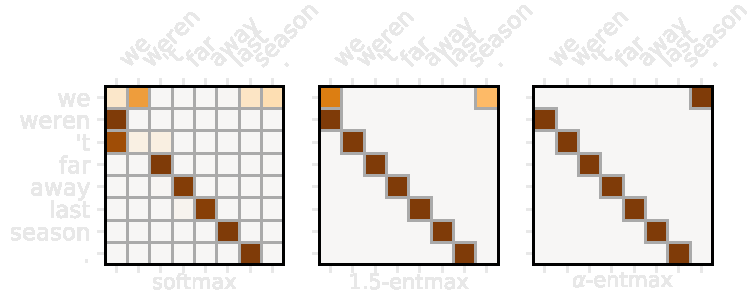
\includegraphics[width=0.9\columnwidth]{figures/head_prev_mybg}\\
        \fontsize{12pt}{15}\selectfont
    \end{center}

\end{frame}

% \begin{frame}
%     \frametitle{Deteção de frases interrogativas}
%     \vspace{-0.5cm}
%     \begin{center}
%         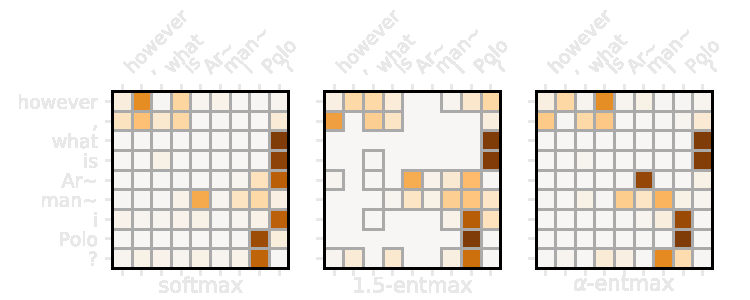
\includegraphics[width=0.9\columnwidth]{figures/head_interro_mybg}\\
%         \fontsize{12pt}{15}\selectfont
%     \end{center}

% \end{frame}

\begin{frame}[fragile]
    \frametitle{Ideias-chave}
    \fontsize{12pt}{14}\selectfont%
    \vspace*{-1cm}
    \begin{center}
        Introduzimos uma forma de usar {\color{tPeony} esparsidade adaptativa} \\
        em redes neuronais, melhorando a {\color{myDarkYellow} transparência} das mesmas.
    \end{center}
    %
    %
    \vfill
    %
    %
    \begin{columns}[T]
        \small
        \begin{column}{.45\textwidth}
            \centering
            \uncover<2->{
                \textbf{\emph{esparsidade}}\\[.5\baselineskip]
                \vspace{0.2cm}
                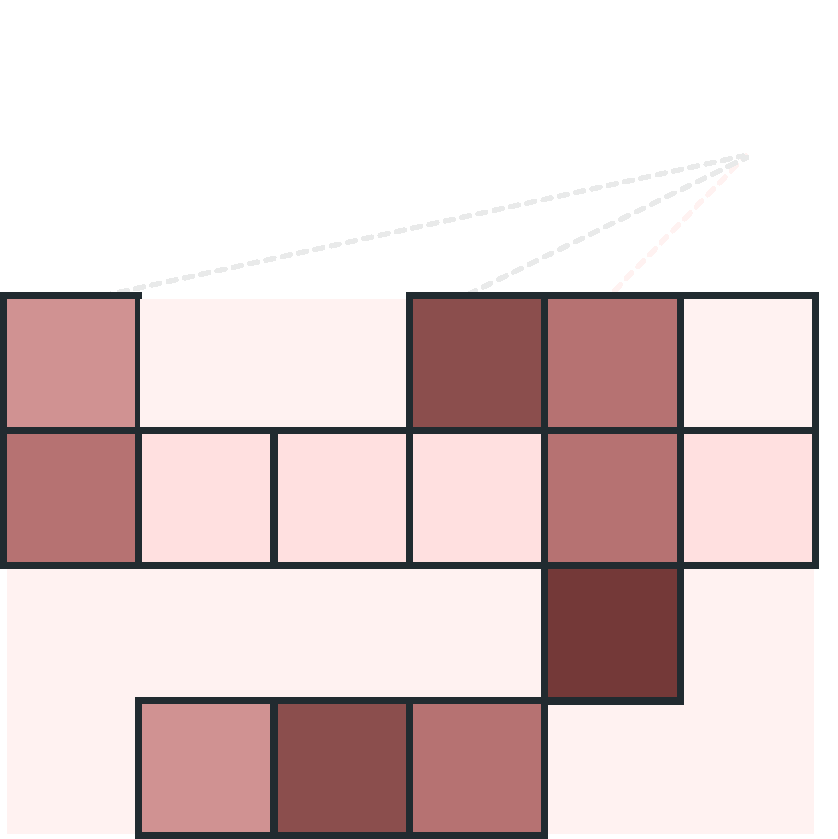
\includegraphics[width=.5\textwidth]{figures/adaptive_sparsity}}%
        \end{column}
        \begin{column}{.45\textwidth}
            \centering
            \uncover<3->{
                \textbf{\emph{mais interpretável}}\\[\baselineskip]
                \vspace{-0.2cm}
                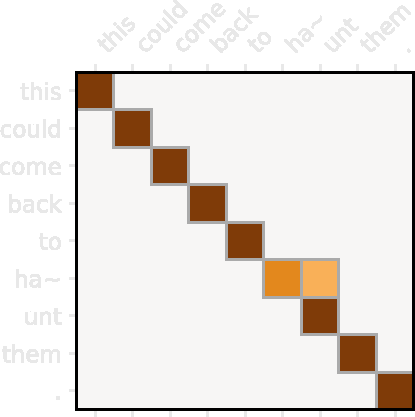
\includegraphics[width=.6\textwidth]{figures/bpe4}}
        \end{column}
    \end{columns}

\end{frame}

\section{Efficient Marg. of Discrete Latent Variables via Sparsity}

% \begin{frame}
%     \frametitle{Latent variable models}
%     \fontsize{12pt}{15}\selectfont

%     \begin{columns}
%         \hspace{-0.5cm}\vspace{-1cm}\begin{column}{0.75\columnwidth}\vspace{-1cm}
%             \begin{itemize}
%                 \uncover<1->{\item[] We focus on latent variables $z$ that are }\uncover<2->{{\color{tPeony} discrete}}\uncover<3->{ or {\color{tBlue} structured}}
%             \end{itemize}

%             \begin{itemize}
%                 \uncover<4->{\item[] $\pi(z | x, \theta)$: distribution over possible $z$}
%             \end{itemize}

%             % besides this, there's also
%             \begin{itemize}
%                 \uncover<7->{\item[] $\ell(x, z; \theta)$: downstream loss: ELBO, Log-Likelihood, (...)}
%             \end{itemize}

%         \end{column}

%         \begin{column}{0.2\columnwidth}
%             \vspace{-0.5cm}
%             \begin{center}
%                 \begin{figure}[ht]
%                     \begin{tikzpicture}
%                         % DISCRETE
%                         \uncover<2->{\draw[draw=tPink,fill=tPink] (1.4,2) circle (0.2) node[anchor=south, yshift=2mm] {{\visible<5->{\color{tPeony} \small 0.2}}};}
%                         \uncover<2->{\draw[draw=tSlateBlue,fill=tSlateBlue] (2,2) circle (0.2) node[anchor=south, yshift=2mm] {{\visible<5->{\color{tPeony} \small 0.6}}};}
%                         \uncover<2->{\draw[draw=tGreen,fill=tGreen] (2.6,2) circle (0.2) node[anchor=south, yshift=2mm] {{\visible<5->{\color{tPeony} \small 0.1}}};}

%                         % STRUCTURE
%                         \uncover<3->{\draw[draw=tSlateBlue,fill=tSlateBlue] (1.4,1) circle (0.2) node[anchor=east, xshift=-2mm] {$[$};}
%                         \uncover<3->{\draw[draw=tGreen,fill=tGreen] (2,1) circle (0.2);}
%                         \uncover<3->{\draw[draw=tPink,fill=tPink] (2.6,1) circle (0.2)
%                             node[anchor=west, xshift=2mm] {$]$}
%                             node[anchor=west, xshift=5mm] {{\visible<6->{\color{tVividBlue} \small 0.4}}};}

%                         \uncover<3->{\draw[draw=tPink,fill=tPink] (1.4,0.5) circle (0.2) node[anchor=east, xshift=-2mm] {$[$};}
%                         \uncover<3->{\draw[draw=tSlateBlue,fill=tSlateBlue] (2,0.5) circle (0.2) node[anchor=north, yshift=-4mm] {\large \bf $\ldots$};}
%                         \uncover<3->{\draw[draw=tGreen,fill=tGreen] (2.6,0.5) circle (0.2)
%                             node[anchor=west, xshift=2mm] {$]$}
%                             node[anchor=west, xshift=5mm] {{\visible<6->{\color{tVividBlue} \small 0.05}}};}

%                         \uncover<3->{\draw[draw=tGreen,fill=tGreen] (1.4,-0.5) circle (0.2) node[anchor=east, xshift=-2mm] {$[$};}
%                         \uncover<3->{\draw[draw=tSlateBlue,fill=tSlateBlue] (2,-0.5) circle (0.2);}
%                         \uncover<3->{\draw[draw=tPink,fill=tPink] (2.6,-0.5) circle (0.2)
%                             node[anchor=west, xshift=2mm] {$]$}
%                             node[anchor=west, xshift=5mm] {{\visible<6->{\color{tVividBlue} \small 0.3}}};}
%                     \end{tikzpicture}
%                 \end{figure}
%             \end{center}
%         \end{column}
%     \end{columns}

%     \vspace{-0.5cm}

%     \begin{itemize}
%         \uncover<8->{\item[] To train, we need to compute the following expectation:}
%     \end{itemize}

%     \begin{equation*}\label{eq:fit1}
%         \uncover<9->{\mathcal{L}_{x}(\theta) =
%             \sum_{z \in \mathcal Z}
%             \pi(z | x, \theta)
%             ~\ell(x, z; \theta)}
%     \end{equation*}

%     \begin{itemize}
%         \uncover<10->
%         {\item[] If $\mathcal Z$ is
%             \only<10>{{\color{tPeony} large}, this sum can get very expensive due to $\ell(x, z; \theta)$!\quad\emoji{oface}}
%             \only<11->{{\color{tVividBlue} combinatorial}, this can be intractable to compute!\quad\emoji{oface}\enspace\emoji{oface}\enspace\emoji{oface}}}
%     \end{itemize}

% \end{frame}

\begin{frame}
    \only<-6>{\frametitle{Soluções anteriores}}\only<7->{\frametitle{{\color{tPeony} A nossa solução}}}
    %\framesubtitle{Using emergent communication as example}
    \fontsize{12pt}{15}\selectfont
    \begin{columns}
        \begin{column}{0.4\columnwidth}
            \centering

            \only<4->{\vspace{-0.8cm}}
            \only<1>{
\includegraphics[width=0.8\columnwidth]{figures/robots-messages-3.pdf}}
            \only<2>{
\includegraphics[width=0.8\columnwidth]{figures/robots-messages-2.pdf}}
            \only<3>{
\includegraphics[width=0.8\columnwidth]{figures/robots-messages-1.pdf}}
            \only<4-5>{
\includegraphics[width=0.8\columnwidth]{figures/envelopes_dense.png}}
            \only<6>{
\includegraphics[width=0.8\columnwidth]{figures/envelopes_sfe.png}}
            %\only<8>{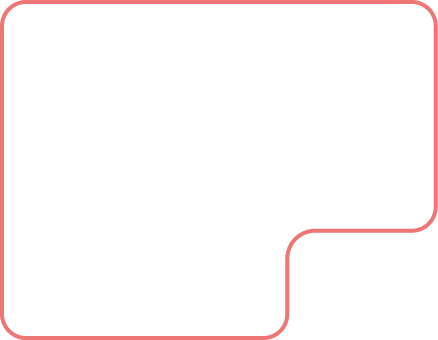
\includegraphics[width=0.9\columnwidth]{figures/envelopes_gumbel.png}}
            \only<7>{
\includegraphics[width=0.8\columnwidth]{figures/envelopes_dense.png}}
            \only<8-11>{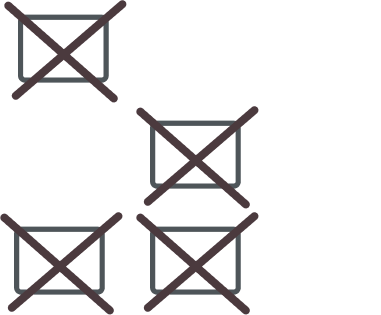
\includegraphics[width=0.8\columnwidth]{figures/envelopes_sparse.png}}

        \end{column}
        \begin{column}{0.55\columnwidth}

            \vspace{-0.8cm}
            \small%
            \only<1-10>{
                \begin{center}
                    \begin{tabular}{lr@{~}lr}
                        \toprule
                        Método                                  & \multicolumn{2}{c}{sucesso (\%)} & \# mensagens                             \\
                        \midrule
                        {\emph{Monte Carlo}}                    &                                  &                                &        \\
                        \uncover<6->{SFE                        & $33.05$                          & {\tiny\color{gray}$\pm 2.84$}  & $1$}   \\
                        %\uncover<7->{SFE$+$                     & $44.32$                          & {\tiny\color{gray}$\pm 2.72$}  & $2$}   \\
                        %\uncover<8->{Gumbel                     & $23.51$                          & {\tiny\color{gray}$\pm 16.19$} & $1$}   \\
                        \midrule
                        \emph{Marginalização}                  &                                  &                                &        \\
                        \uncover<5->{Denso                      & $93.37$                          & {\tiny\color{gray}$\pm 0.42$}  & $256$} \\
                        \uncover<7->{\textcolor{tPeony}{Esparso} &
                        \uncover<9->{$93.35$                   & {\tiny\color{gray}$\pm 0.50$}}   &
                        \uncover<10->{$3.13${\tiny\color{gray}$\pm 0.48$}} }                                                                 \\
                        \bottomrule
                    \end{tabular}
                \end{center}
            }
            \only<11->{
                \begin{center}
                    % This file was created by tikzplotlib v0.9.4.
\begin{tikzpicture}
    \colorlet{color0}{myDarkYellow}
    \colorlet{color1}{tPeony}
    \colorlet{color2}{tBlue}
    \begin{axis}[
            scale=.55,
            legend cell align={left},
            legend style={fill opacity=0.1, draw opacity=1, text opacity=1, at={(0.95,0.5)}, anchor=east},
            tick align=outside,
            tick pos=left,
            x grid style={white!69.0196078431373!black},
            xlabel={Epoch},
            xmin=-4.975, xmax=104.475,
            xtick style={color=black},
            y grid style={white!69.0196078431373!black},
            ylabel={\# messages},
            ymin=-20, ymax=300,
            ytick style={color=gray},
            ytick={1, 100, 200, 256}
        ]
        \addplot [semithick, color1, mark=*, mark size=0, mark options={solid}]
        table {%
                0 202.050897277228
                1 88.2360767326733
                2 33.7467512376238
                3 24.1506806930693
                4 18.9990717821782
                5 15.8439047029703
                6 13.6591893564356
                7 12.4175433168317
                8 11.3674195544554
                9 10.4839108910891
                10 9.85380569306931
                11 9.15037128712871
                12 8.62407178217822
                13 8.36262376237624
                14 8.02475247524752
                15 7.61943069306931
                16 7.48901608910891
                17 7.19538985148515
                18 6.92821782178218
                19 6.71318069306931
                20 6.49350247524752
                21 6.32193688118812
                22 6.25819925742574
                23 6.05290841584158
                24 5.93115717821782
                25 5.75897277227723
                26 5.66970915841584
                27 5.55105198019802
                28 5.46116955445545
                29 5.38273514851485
                30 5.29022277227723
                31 5.15965346534653
                32 5.1304146039604
                33 5.09467821782178
                34 5
                35 4.9060952970297
                36 4.89232673267327
                37 4.82781559405941
                38 4.72880569306931
                39 4.67558787128713
                40 4.62345297029703
                41 4.56822400990099
                42 4.51129331683168
                43 4.50866336633663
                44 4.48406559405941
                45 4.37438118811881
                46 4.35488861386139
                47 4.32224628712871
                48 4.26763613861386
                49 4.20606435643564
                50 4.16089108910891
                51 4.19229579207921
                52 4.09483292079208
                53 4.08431311881188
                54 4.06373762376238
                55 4.00928217821782
                56 3.9789603960396
                57 3.92527846534653
                58 3.92852722772277
                59 3.91181930693069
                60 3.87345297029703
                61 3.83369430693069
                62 3.80600247524752
                63 3.77413366336634
                64 3.76608910891089
                65 3.75665222772277
                66 3.71163366336634
                67 3.69848391089109
                68 3.65903465346535
                69 3.62685643564356
                70 3.59204826732673
                71 3.60117574257426
                72 3.55553836633663
                73 3.55383663366337
                74 3.52939356435644
                75 3.50340346534653
                76 3.45436262376238
                77 3.44183168316832
                78 3.41058168316832
                79 3.45126856435644
                80 3.3957301980198
                81 3.39944306930693
                82 3.33818069306931
                83 3.32224628712871
                84 3.30940594059406
                85 3.30290841584158
                86 3.30306311881188
                87 3.28558168316832
                88 3.27150371287129
                89 3.21642945544554
                90 3.18409653465347
                91 3.18270420792079
                92 3.18409653465347
                93 3.15872524752475
                94 3.1460396039604
                95 3.14016089108911
                96 3.11633663366337
                97 3.09112004950495
                98 3.14990717821782
                99 3.09467821782178
            };
        \addlegendentry{sparsemax}
        \path [draw=color0, semithick]
        (axis cs:1,1)
        --(axis cs:99.5,1);
        \path [draw=color2, semithick]
        (axis cs:1,256)
        --(axis cs:99.5,256);
        \addlegendimage{no markers,color0}
        \addlegendimage{no markers,color2}
        \addlegendentry{SFE, etc}
        \addlegendentry{softmax}
    \end{axis}
\end{tikzpicture}


                \end{center}
            }
        \end{column}
    \end{columns}
    % \vspace{0.2cm}
    % \begin{itemize}
    %     \uncover<14->{\item[] We use {\color{tPeony} sparsemax}, {\color{tVividBlue} top-$k$ sparsemax} and {\color{tVividBlue} SparseMAP} to allow efficient marginalization}
    % \end{itemize}

\end{frame}

% \begin{frame}
%     \frametitle{Results}
%     \fontsize{14pt}{15}\selectfont
%     \begin{itemize}
%         \uncover<1->{\item[] We test our methods for models with discrete latent variables,}
%             \begin{itemize}
%                 \uncover<2->{\item Semi-Supervised VAE}
%                       \uncover<3->{\item Emergent communication}
%             \end{itemize}
%             \uncover<4->{\item[] but also in models with an exponentially large set of $\mathcal Z$,}
%             \begin{itemize}
%                 \uncover<5->{\item Bit-vector VAE}
%             \end{itemize}
%     \end{itemize}

%     \begin{itemize}
%         \uncover<6->{\item[] Our methods are top-performers and efficient!}
%     \end{itemize}
% \end{frame}

\begin{frame}
    \frametitle{Ideias-chave}

    \centering\fontsize{14pt}{14}\selectfont%
    Introduzimos um novo método\\
    para treinar, de forma mais eficiente, redes {\color{myDarkYellow} compactas},\\
    usando {\color{tPeony} esparsidade}.
    %
    %
    \vfill
    %
    %
    \begin{columns}[T]
        \small
        \begin{column}{.45\textwidth}
            \centering
            \vspace{-1em}
            \uncover<2->{
                \textbf{\emph{eficiente}}\\[\baselineskip]
                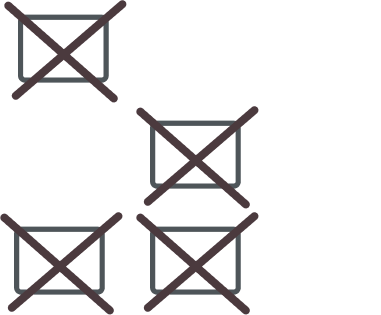
\includegraphics[width=0.65\columnwidth]{figures/envelopes_sparse.png}
            }
        \end{column}
        \begin{column}{.45\textwidth}
            \centering
            \uncover<3->{
                \textbf{\emph{esparso, se necessário}}\\[\baselineskip]
                % This file was created by tikzplotlib v0.9.4.
\small
\begin{tikzpicture}
    ​
    \colorlet{color0}{tYellow}
    \colorlet{color1}{tPeony}
    \colorlet{color2}{tTarmac}
    ​
    \begin{axis}[
            scale=.45,
            legend cell align={left},
            legend style={fill opacity=0.1, draw opacity=1, text opacity=1},
            tick align=outside,
            tick pos=left,
            x grid style={white!69.0196078431373!black},
            xlabel={Epoch},
            xmin=-4.975, xmax=104.475,
            xtick style={color=black},
            y grid style={white!69.0196078431373!black},
            ylabel={\# messages},
            ymin=-9.90855198019802, ymax=260,
            ytick style={color=gray},
            ytick={1, 100, 200, 256}
        ]
        \addplot [semithick, color1, mark=*, mark size=0, mark options={solid}]
        table {%
                0 202.050897277228
                1 88.2360767326733
                2 33.7467512376238
                3 24.1506806930693
                4 18.9990717821782
                5 15.8439047029703
                6 13.6591893564356
                7 12.4175433168317
                8 11.3674195544554
                9 10.4839108910891
                10 9.85380569306931
                11 9.15037128712871
                12 8.62407178217822
                13 8.36262376237624
                14 8.02475247524752
                15 7.61943069306931
                16 7.48901608910891
                17 7.19538985148515
                18 6.92821782178218
                19 6.71318069306931
                20 6.49350247524752
                21 6.32193688118812
                22 6.25819925742574
                23 6.05290841584158
                24 5.93115717821782
                25 5.75897277227723
                26 5.66970915841584
                27 5.55105198019802
                28 5.46116955445545
                29 5.38273514851485
                30 5.29022277227723
                31 5.15965346534653
                32 5.1304146039604
                33 5.09467821782178
                34 5
                35 4.9060952970297
                36 4.89232673267327
                37 4.82781559405941
                38 4.72880569306931
                39 4.67558787128713
                40 4.62345297029703
                41 4.56822400990099
                42 4.51129331683168
                43 4.50866336633663
                44 4.48406559405941
                45 4.37438118811881
                46 4.35488861386139
                47 4.32224628712871
                48 4.26763613861386
                49 4.20606435643564
                50 4.16089108910891
                51 4.19229579207921
                52 4.09483292079208
                53 4.08431311881188
                54 4.06373762376238
                55 4.00928217821782
                56 3.9789603960396
                57 3.92527846534653
                58 3.92852722772277
                59 3.91181930693069
                60 3.87345297029703
                61 3.83369430693069
                62 3.80600247524752
                63 3.77413366336634
                64 3.76608910891089
                65 3.75665222772277
                66 3.71163366336634
                67 3.69848391089109
                68 3.65903465346535
                69 3.62685643564356
                70 3.59204826732673
                71 3.60117574257426
                72 3.55553836633663
                73 3.55383663366337
                74 3.52939356435644
                75 3.50340346534653
                76 3.45436262376238
                77 3.44183168316832
                78 3.41058168316832
                79 3.45126856435644
                80 3.3957301980198
                81 3.39944306930693
                82 3.33818069306931
                83 3.32224628712871
                84 3.30940594059406
                85 3.30290841584158
                86 3.30306311881188
                87 3.28558168316832
                88 3.27150371287129
                89 3.21642945544554
                90 3.18409653465347
                91 3.18270420792079
                92 3.18409653465347
                93 3.15872524752475
                94 3.1460396039604
                95 3.14016089108911
                96 3.11633663366337
                97 3.09112004950495
                98 3.14990717821782
                99 3.09467821782178
            };
        \addlegendentry{sparsemax}
        \addplot [semithick, color1, opacity=0.5, dotted, forget plot]
        table {%
                0 162.392821782178
                1 70.0446472772277
                2 22.5818069306931
                3 17.8559715346535
                4 14.9709158415842
                5 12.9856745049505
                6 11.6587252475248
                7 10.6594368811881
                8 9.76274752475248
                9 9.09211014851485
                10 8.53991336633663
                11 8.10751856435644
                12 7.65931311881188
                13 7.3685952970297
                14 7.11302599009901
                15 6.80179455445545
                16 6.52422648514851
                17 6.41271658415842
                18 6.21970915841584
                19 6.01324257425743
                20 5.8689047029703
                21 5.72277227722772
                22 5.64043935643564
                23 5.56986386138614
                24 5.39012995049505
                25 5.31358292079208
                26 5.18610767326733
                27 5.10971534653465
                28 4.96293316831683
                29 4.91073638613861
                30 4.86116955445544
                31 4.79071782178218
                32 4.70340346534653
                33 4.64272896039604
                34 4.54876237623762
                35 4.48165222772277
                36 4.42181311881188
                37 4.37679455445545
                38 4.31002475247525
                39 4.275
                40 4.21772896039604
                41 4.16067450495049
                42 4.13273514851485
                43 4.0823948019802
                44 4.03991336633663
                45 4.01878094059406
                46 3.946875
                47 3.92571163366337
                48 3.8491646039604
                49 3.84897896039604
                50 3.8144801980198
                51 3.76856435643564
                52 3.72193688118812
                53 3.73898514851485
                54 3.7177599009901
                55 3.65399133663366
                56 3.63205445544554
                57 3.60903465346535
                58 3.55553836633663
                59 3.53802599009901
                60 3.49554455445545
                61 3.46407797029703
                62 3.45340346534653
                63 3.44662747524753
                64 3.4208849009901
                65 3.38814975247525
                66 3.3480198019802
                67 3.30572400990099
                68 3.3039603960396
                69 3.25863242574257
                70 3.25402227722772
                71 3.26800742574257
                72 3.25281559405941
                73 3.1950495049505
                74 3.1477103960396
                75 3.19993811881188
                76 3.12865099009901
                77 3.14319306930693
                78 3.12923886138614
                79 3.12141089108911
                80 3.07162747524752
                81 3.06522277227723
                82 3.06280940594059
                83 3.03090965346535
                84 2.9957301980198
                85 3.01522277227723
                86 2.98007425742574
                87 2.94594678217822
                88 2.95383663366337
                89 2.95324876237624
                90 2.9259900990099
                91 2.91011757425743
                92 2.89136757425743
                93 2.8904702970297
                94 2.88542698019802
                95 2.87317450495049
                96 2.79743193069307
                97 2.80145420792079
                98 2.81998762376238
                99 2.80272277227723
            };
        \addplot [semithick, color1, opacity=0.5, dotted, forget plot]
        table {%
                0 219.17103960396
                1 164.074412128713
                2 61.8660581683168
                3 40.1205136138614
                4 30.4589108910891
                5 24.0548576732673
                6 21.098452970297
                7 18.6735148514851
                8 17.4169863861386
                9 16.6282178217822
                10 15.403650990099
                11 14.2937809405941
                12 13.2836633663366
                13 12.4058787128713
                14 11.7689665841584
                15 11.1133663366337
                16 10.6939665841584
                17 10.3084158415842
                18 10.0227722772277
                19 9.63415841584159
                20 9.42156559405941
                21 9.16738861386139
                22 8.94415222772277
                23 8.68709777227723
                24 8.36271658415842
                25 8.27097772277228
                26 7.96188118811881
                27 7.74427599009901
                28 7.55247524752475
                29 7.29266707920792
                30 7.18400371287129
                31 6.94631806930693
                32 6.85216584158416
                33 6.70207301980198
                34 6.4967202970297
                35 6.32722772277228
                36 6.17735148514851
                37 6.13316831683168
                38 6.01596534653465
                39 5.84876237623762
                40 5.80389851485149
                41 5.68570544554456
                42 5.66726485148515
                43 5.4792698019802
                44 5.43171410891089
                45 5.4064047029703
                46 5.24600866336634
                47 5.15578589108911
                48 5.10649752475248
                49 5.09860767326733
                50 4.97144183168317
                51 4.91336633663366
                52 4.87930074257426
                53 4.78842821782178
                54 4.76098391089109
                55 4.67243193069307
                56 4.65219678217822
                57 4.62849628712871
                58 4.61497524752475
                59 4.53886138613861
                60 4.43663366336634
                61 4.36698638613861
                62 4.32691831683168
                63 4.34347153465346
                64 4.29737004950495
                65 4.23576732673267
                66 4.21466584158416
                67 4.1448948019802
                68 4.16472772277228
                69 4.1009900990099
                70 4.05278465346535
                71 4.03997524752475
                72 3.95748762376238
                73 4.01082920792079
                74 3.9478650990099
                75 3.89118193069307
                76 3.86689356435644
                77 3.85569306930693
                78 3.79690594059406
                79 3.78524133663366
                80 3.76748143564356
                81 3.77085396039604
                82 3.72100866336634
                83 3.70139232673267
                84 3.70315594059406
                85 3.68245668316832
                86 3.6439047029703
                87 3.59217202970297
                88 3.6147896039604
                89 3.55962252475248
                90 3.56726485148515
                91 3.52778465346535
                92 3.51386138613861
                93 3.49990717821782
                94 3.46565594059406
                95 3.47450495049505
                96 3.45281559405941
                97 3.44189356435644
                98 3.41268564356436
                99 3.40003094059406
            };
        \path [draw=color0, semithick]
        (axis cs:1,1)
        --(axis cs:99.5,1);
        \path [draw=color2, semithick]
        (axis cs:1,256)
        --(axis cs:99.5,256);
        \addlegendimage{no markers,color0}
        \addlegendimage{no markers,color2}
        \addlegendentry{SFE, etc}
        \addlegendentry{softmax}
    \end{axis}
\end{tikzpicture}

}
        \end{column}
    \end{columns}
\end{frame}

\section{Impacto e Conclusões}

\begin{frame}
    \frametitle{Impacto}
    \centering
    \fontsize{12pt}{15}\selectfont
    \begin{columns}[T]
    \begin{column}{.7\textwidth}
    \begin{itemize}
        \uncover<2->{\item Artigos que desenvolveram mais métodos com {\color{tPeony} esparsidade},
        focados na transparência e eficiência que isso traz}
        \uncover<3->{\item Esperamos que este trabalho tenha contribuído para IA mais responsável}
    \end{itemize}
\end{column}
    \begin{column}{.25\textwidth}
        \centering
        \uncover<4->{
            
\includegraphics[width=0.8\columnwidth]{figures/crai.png}
        }
    \end{column}
    \end{columns}
\end{frame}

\begin{frame}
    \frametitle{Conclusões}
    \centering\fontsize{14pt}{14}\selectfont%
    Com {\color{tPeony} esparsidade}, démos passos\\
    para levar modelos neuronais mais perto da versão 2.0\\
    %
    %
    \vfill
    %
    %
    \begin{columns}[T]
        \small
        \begin{column}{.45\textwidth}
            \centering
            \uncover<2->{
                {\color{myDarkYellow} \textbf{\emph{transparência}}}\\[\baselineskip]
                \vspace{0.2cm}
                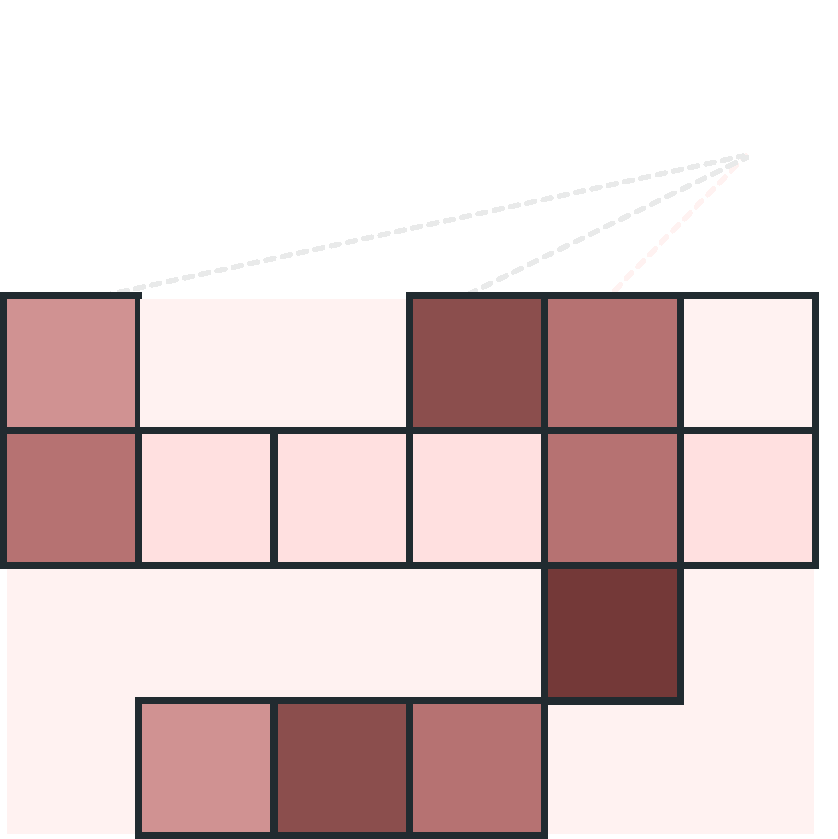
\includegraphics[width=.45\textwidth]{figures/adaptive_sparsity}}%
        \end{column}
        \begin{column}{.45\textwidth}
            \centering
            \uncover<3->{
                \textbf{\emph{mais {\color{myDarkYellow} compacto}}}\\[\baselineskip]
                \vspace{-0.5em}
                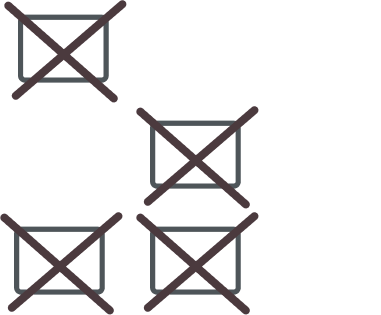
\includegraphics[width=0.65\columnwidth]{figures/envelopes_sparse.png}
            }
        \end{column}
    \end{columns}

    \vfill
    \centering
    {\scriptsize
        \color{mygr}
        \begin{tabular}{r@{~}l@{\quad}r@{~}l}
            \raisebox{-0.7mm}[\height][\depth]{\emoji{githubfg}} & \href{https://github.com/deep-spin}{\tt github.com/deep-spin} &
            \raisebox{-0.4mm}[\height][\depth]{\emoji{home}}     & \href{https://goncalomcorreia.com}{\tt goncalomcorreia.com}
        \end{tabular}}
\end{frame}

\begin{frame}[plain,c, noframenumbering]
    %\frametitle{A first slide}
    \begin{center}
    \Huge Agradecimentos
    \end{center}
\end{frame}

% \begin{frame}[t,allowframebreaks,noframenumbering, plain]
%     \frametitle{References}
%     \printbibliography
% \end{frame}

% \begin{frame}[noframenumbering, plain]
%     \frametitle{Parameter sharing analysis}
%     \begin{table}[htbp]
%         \centering
%         \begin{tabular}{lcc}
%             \toprule
%                                                                & TER$\downarrow$ & BLEU$\uparrow$ \\
%             MT Baseline                                        & 24.76           & 62.11          \\
%             Transformer                                        & 27.80           & 60.76          \\
%             \midrule
%             Transformer decoder                                & 20.33           & 69.31          \\
%             Pre-trained BERT                                   & 20.83           & 69.11          \\
%             \hspace{1ex}\textcolor{gray}{\textit{with}}
%             CA $\leftarrow$ SA                                 & 18.91           & 71.81          \\
%             \textover[r]
%             {\hspace{1ex}\textcolor{gray}{\textit{and}}}{\hspace{1ex}\textit{with}}
%             \textover[r]
%             {SA $\leftrightarrow$}
%             {CA $\leftarrow$} Encoder SA                       & \textbf{18.44}  & \textbf{72.25} \\
%             \textover[r]
%             {\hspace{1ex}\textcolor{gray}{\textit{and}}}{\hspace{1ex}\textit{with}}
%             \textover[r]
%             {CA $\leftrightarrow$}{CA $\leftarrow$} SA         & 18.75           & 71.83          \\
%             \textover[r]
%             {\hspace{1ex}\textcolor{gray}{\textit{and}}}{\hspace{1ex}\textit{with}}
%             \textover[r]
%             {FF $\leftrightarrow$}{CA $\leftarrow$} Encoder FF & 19.04           & 71.53          \\
%             \bottomrule
%         \end{tabular}
%         \label{tab:ablation_smt}
%     \end{table}
% \end{frame}

% \begin{frame}[noframenumbering, plain]
%     \frametitle{Related Work: Other Sparse Transformers}
%     \cornercite{Child2019,Sukhbaatar2019}

%     \vspace{-1.5cm}
%     \begin{center}
%         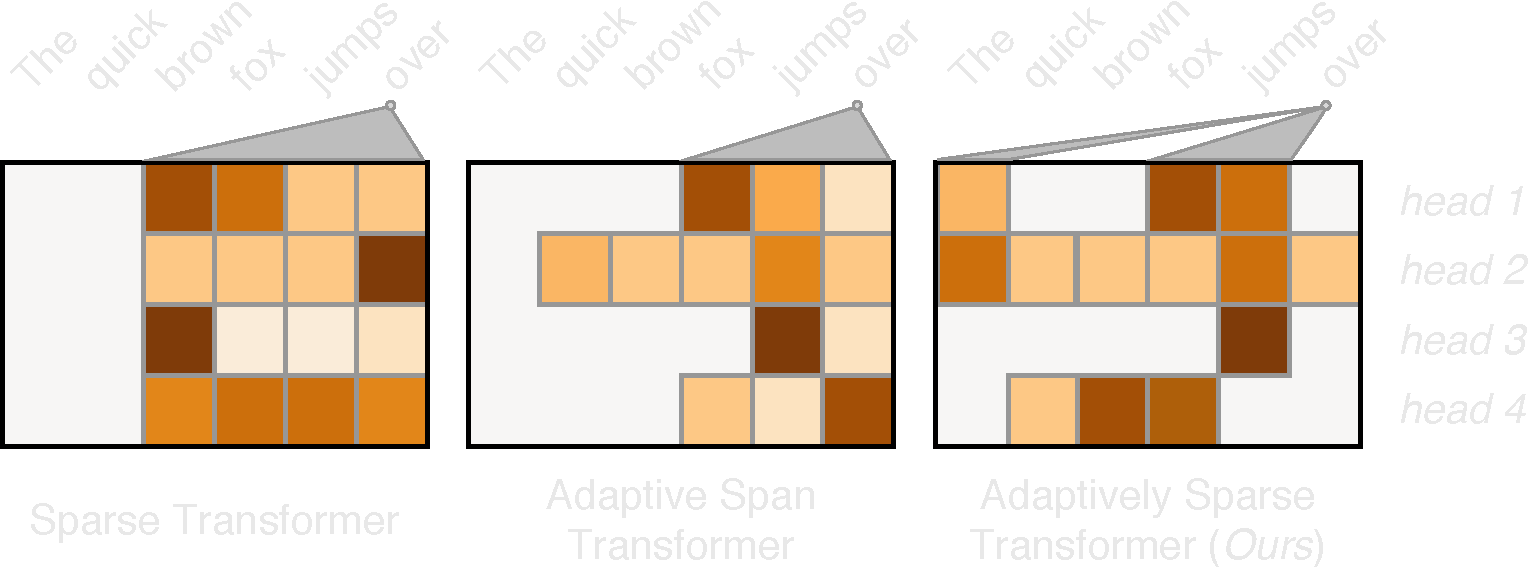
\includegraphics[width=0.7\columnwidth]{figures/comparison_mybg}

%         \bigskip

%         Our model allows {\color{myDarkYellow} non-contiguous} attention for each head.
%     \end{center}

% \end{frame}

% \begin{frame}[noframenumbering, plain]
%     \frametitle{$\Omega$-Regularized Argmax}
%     \cornercite{Niculae2017}
%     \fontsize{12pt}{15}\selectfont
%     \vspace{-0.5cm}
%     \begin{itemize}
%         \item[] For convex $\Omega$, define the {\bf $\Omega$-regularized argmax transformation}:\\
%             \bigskip
%             \begin{center}
%                 $\displaystyle
%                     \argmaxbf{}_{{\Omega}}(\vectsymb{z}) \defeq \arg\max_{\vectsymb{p} \in \triangle} \DP{\vectsymb{z}}{\vectsymb{p}} {\color{tPeony}- \Omega(\vectsymb{p})}$
%             \end{center}
%     \end{itemize}
%     \bigskip
%     \begin{itemize}
%         \uncover<2->{\item {\color{myDarkYellow} Argmax} corresponds to {\bf no regularization}, $\displaystyle\Omega \equiv 0$}
%               \uncover<3->{\item {\color{myDarkYellow} Softmax} amounts to {\bf entropic regularization}, $\displaystyle\Omega(\vectsymb{p}) = \sum_{i=1}^K p_i \log p_i$}
%               \uncover<4->{\item {\color{myDarkYellow} Sparsemax} amounts to {\bf $\ell_2$-regularization}, $\displaystyle\Omega(\vectsymb{p}) = \frac{1}{2}\|\vectsymb{p}\|^2$.}
%     \end{itemize}
%     \bigskip
%     \begin{itemize}
%         \item[] \uncover<5->{Is there something in-between?}
%     \end{itemize}
%     \uncover<4>{\cornercite[south east]{sparsemax}}
% \end{frame}

% \begin{frame}[noframenumbering, plain]
%     \frametitle{BLEU Scores}

%     \begin{table}[ht]
%         \begin{center}
%             \small
%             \resizebox{0.8\columnwidth}{!}{\begin{tabular}{lrrrr}
%                     \toprule
%                     activation
%                      & \langp{de}{en}               & \langp{ja}{en}
%                      & \langp{ro}{en}               & \only<1>{\langp{en}{de}}\only<2->{{\color{tPeony} \langp{en}{de}}} \\
%                     \midrule
%                     $\softmaxlight$
%                      & 29.79
%                      & 21.57
%                      & 32.70
%                      & 26.02                                                                                             \\
%                     $\aentmax[1.5]$
%                      & 29.83
%                      & {\color{myDarkYellow} 22.13}
%                      & {\color{myDarkYellow} 33.10}
%                      & 25.89                                                                                             \\
%                     $\aentmax[\alpha]$
%                      & {\color{myDarkYellow} 29.90}
%                      & 21.74
%                      & 32.89
%                      & {\color{myDarkYellow} 26.93}                                                                      \\
%                     \bottomrule
%                 \end{tabular}}
%         \end{center}
%     \end{table}

%     \bigskip

%     \begin{itemize}
%         \uncover<3>{\item[] For analysis for other language pairs, see Appendix A.}
%     \end{itemize}

% \end{frame}

% \begin{frame}[noframenumbering, plain]
%     \frametitle{Learned $\alpha$}

%     \centering\fontsize{10pt}{15}\selectfont
%     % This file was created by tikzplotlib v0.8.5.
\begin{tikzpicture}

\definecolor{color0}{rgb}{0.12156862745098,0.466666666666667,0.705882352941177}

\begin{groupplot}[group style={group size=3 by 1}]
\nextgroupplot[
width=0.35\columnwidth,
height=0.35\columnwidth,
tick align=outside,
tick pos=left,
x grid style={white!69.01960784313725!black},
xmin=0.95, xmax=2.05,
xtick style={color=black},
y grid style={white!69.01960784313725!black},
title={Encoder
Self-Attention},
ymin=0, ymax=21,
ytick style={color=black}
]
\draw[fill=color0,draw opacity=0] (axis cs:1,0) rectangle (axis cs:1.06666666666667,3);
\draw[fill=color0,draw opacity=0] (axis cs:1.06666666666667,0) rectangle (axis cs:1.13333333333333,11);
\draw[fill=color0,draw opacity=0] (axis cs:1.13333333333333,0) rectangle (axis cs:1.2,4);
\draw[fill=color0,draw opacity=0] (axis cs:1.2,0) rectangle (axis cs:1.26666666666667,6);
\draw[fill=color0,draw opacity=0] (axis cs:1.26666666666667,0) rectangle (axis cs:1.33333333333333,8);
\draw[fill=color0,draw opacity=0] (axis cs:1.33333333333333,0) rectangle (axis cs:1.4,3);
\draw[fill=color0,draw opacity=0] (axis cs:1.4,0) rectangle (axis cs:1.46666666666667,1);
\draw[fill=color0,draw opacity=0] (axis cs:1.46666666666667,0) rectangle (axis cs:1.53333333333333,0);
\draw[fill=color0,draw opacity=0] (axis cs:1.53333333333333,0) rectangle (axis cs:1.6,2);
\draw[fill=color0,draw opacity=0] (axis cs:1.6,0) rectangle (axis cs:1.66666666666667,1);
\draw[fill=color0,draw opacity=0] (axis cs:1.66666666666667,0) rectangle (axis cs:1.73333333333333,0);
\draw[fill=color0,draw opacity=0] (axis cs:1.73333333333333,0) rectangle (axis cs:1.8,0);
\draw[fill=color0,draw opacity=0] (axis cs:1.8,0) rectangle (axis cs:1.86666666666667,2);
\draw[fill=color0,draw opacity=0] (axis cs:1.86666666666667,0) rectangle (axis cs:1.93333333333333,4);
\draw[fill=color0,draw opacity=0] (axis cs:1.93333333333333,0) rectangle (axis cs:2,3);

\nextgroupplot[
width=0.35\columnwidth,
height=0.35\columnwidth,
tick align=outside,
tick pos=left,
x grid style={white!69.01960784313725!black},
xlabel={\(\displaystyle \alpha\)},
xmin=0.95, xmax=2.05,
xtick style={color=black},
y grid style={white!69.01960784313725!black},
title={Context
Attention},
ymin=0, ymax=21,
yticklabels={,,},
ytick style={color=black}
]
\draw[fill=color0,draw opacity=0] (axis cs:1,0) rectangle (axis cs:1.06666666666667,7);
\draw[fill=color0,draw opacity=0] (axis cs:1.06666666666667,0) rectangle (axis cs:1.13333333333333,6);
\draw[fill=color0,draw opacity=0] (axis cs:1.13333333333333,0) rectangle (axis cs:1.2,15);
\draw[fill=color0,draw opacity=0] (axis cs:1.2,0) rectangle (axis cs:1.26666666666667,17);
\draw[fill=color0,draw opacity=0] (axis cs:1.26666666666667,0) rectangle (axis cs:1.33333333333333,3);
\draw[fill=color0,draw opacity=0] (axis cs:1.33333333333333,0) rectangle (axis cs:1.4,0);
\draw[fill=color0,draw opacity=0] (axis cs:1.4,0) rectangle (axis cs:1.46666666666667,0);
\draw[fill=color0,draw opacity=0] (axis cs:1.46666666666667,0) rectangle (axis cs:1.53333333333333,0);
\draw[fill=color0,draw opacity=0] (axis cs:1.53333333333333,0) rectangle (axis cs:1.6,0);
\draw[fill=color0,draw opacity=0] (axis cs:1.6,0) rectangle (axis cs:1.66666666666667,0);
\draw[fill=color0,draw opacity=0] (axis cs:1.66666666666667,0) rectangle (axis cs:1.73333333333333,0);
\draw[fill=color0,draw opacity=0] (axis cs:1.73333333333333,0) rectangle (axis cs:1.8,0);
\draw[fill=color0,draw opacity=0] (axis cs:1.8,0) rectangle (axis cs:1.86666666666667,0);
\draw[fill=color0,draw opacity=0] (axis cs:1.86666666666667,0) rectangle (axis cs:1.93333333333333,0);
\draw[fill=color0,draw opacity=0] (axis cs:1.93333333333333,0) rectangle (axis cs:2,0);

\nextgroupplot[
width=0.35\columnwidth,
height=0.35\columnwidth,
tick align=outside,
tick pos=left,
x grid style={white!69.01960784313725!black},
xmin=0.95, xmax=2.05,
xtick style={color=black},
y grid style={white!69.01960784313725!black},
title={Decoder
Self-Attention},
ymin=0, ymax=21,
yticklabels={,,},
ytick style={color=black}
]
\draw[fill=color0,draw opacity=0] (axis cs:1,0) rectangle (axis cs:1.06666666666667,3);
\draw[fill=color0,draw opacity=0] (axis cs:1.06666666666667,0) rectangle (axis cs:1.13333333333333,6);
\draw[fill=color0,draw opacity=0] (axis cs:1.13333333333333,0) rectangle (axis cs:1.2,20);
\draw[fill=color0,draw opacity=0] (axis cs:1.2,0) rectangle (axis cs:1.26666666666667,10);
\draw[fill=color0,draw opacity=0] (axis cs:1.26666666666667,0) rectangle (axis cs:1.33333333333333,2);
\draw[fill=color0,draw opacity=0] (axis cs:1.33333333333333,0) rectangle (axis cs:1.4,3);
\draw[fill=color0,draw opacity=0] (axis cs:1.4,0) rectangle (axis cs:1.46666666666667,2);
\draw[fill=color0,draw opacity=0] (axis cs:1.46666666666667,0) rectangle (axis cs:1.53333333333333,1);
\draw[fill=color0,draw opacity=0] (axis cs:1.53333333333333,0) rectangle (axis cs:1.6,0);
\draw[fill=color0,draw opacity=0] (axis cs:1.6,0) rectangle (axis cs:1.66666666666667,0);
\draw[fill=color0,draw opacity=0] (axis cs:1.66666666666667,0) rectangle (axis cs:1.73333333333333,1);
\draw[fill=color0,draw opacity=0] (axis cs:1.73333333333333,0) rectangle (axis cs:1.8,0);
\draw[fill=color0,draw opacity=0] (axis cs:1.8,0) rectangle (axis cs:1.86666666666667,0);
\draw[fill=color0,draw opacity=0] (axis cs:1.86666666666667,0) rectangle (axis cs:1.93333333333333,0);
\draw[fill=color0,draw opacity=0] (axis cs:1.93333333333333,0) rectangle (axis cs:2,0);
\end{groupplot}

\end{tikzpicture}


%     \bigskip

%     \fontsize{12pt}{15}\selectfont
%     Bimodal for the encoder, mostly unimodal for the decoder.

% \end{frame}

% \begin{frame}[noframenumbering, plain]
%     \frametitle{Subword-Merging Head}
%     \vspace{-0.7cm}
%     \begin{columns}[T]
%         \small
%         \begin{column}{.33\textwidth}
%             \vspace{-0.1cm}
%             \centering
%             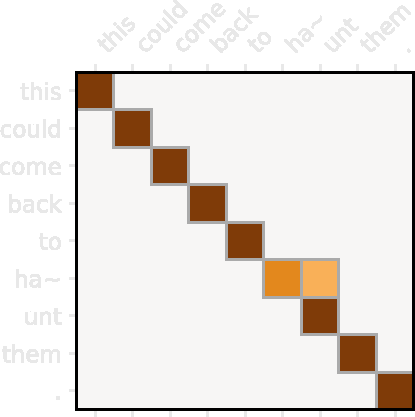
\includegraphics[width=0.9\columnwidth]{figures/bpe4}
%         \end{column}
%         \begin{column}{.33\textwidth}
%             \vspace{-0.2cm}
%             \centering
%             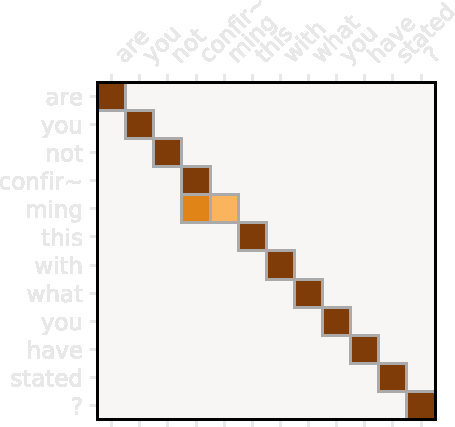
\includegraphics[width=\columnwidth]{figures/bpe3}
%         \end{column}
%         \begin{column}{.33\textwidth}
%             \centering
%             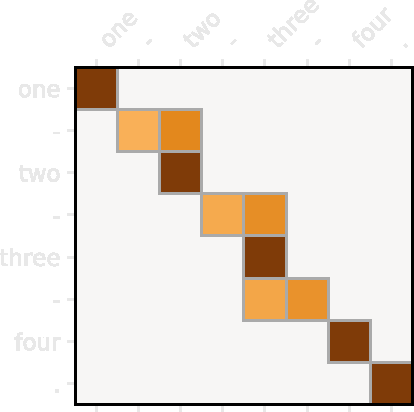
\includegraphics[width=0.9\columnwidth]{figures/bpe2}
%         \end{column}
%     \end{columns}

%     \begin{center}
%         \fontsize{12pt}{15}\selectfont
%         Learned {\color{myDarkYellow}$\alpha = 1.91$}.
%     \end{center}

% \end{frame}

% \begin{frame}[noframenumbering, plain]
%     \frametitle{Semi-Supervised VAE}%\cornerciteme{sparsemarg}

%     \newcommand*\parcolor{myfg}
%     \newcommand*\clfcolor{myfg}
%     \newcommand*\colParseZero{mybg}
%     \newcommand*\colParseNonz{mybg}
%     \renewcommand*\parcolor{tPeony}
%     \renewcommand*\clfcolor{tYellow}

%     \begin{align*}
%         \mathcal{L}_{x}(\theta) & =
%         \tikzmark{sum}\sum_{z \in \mathcal{Z}}
%         \textcolor{\parcolor}{\pi\tikzmark{parp}(z | x)}~
%         \textcolor{\clfcolor}{\ell\tikzmark{clfp}(x, z)}                                   \\
%                                 & = \mathbb{E}_{z \sim \textcolor{\parcolor}{\pi(z | x)}}~ %
%         \textcolor{\clfcolor}{\ell(x, z)}
%     \end{align*}

%     \vspace{\baselineskip}
%     \begin{itemize}
%         \item<1-> Semi-Supervised VAE on MNIST: $z$ is one of 10 categories
%         \item<4-> Train this with 10\% labeled data
%     \end{itemize}
%     \begin{tikzpicture}[%
%             remember picture,
%             overlay,
%             expl/.style={font=\small}]
%         \uncover<2->{
%             \node[expl,anchor=north east] (explpar)
%             at ($(current page.north east) - (.5, 2.0)$)
%             {Gaussian VAE};
%             \path (explpar.west) edge[->,very thick,bend right] ([yshift=2.0ex]{pic cs:clfp});
%         }
%         %
%         \uncover<3->{
%             \node[expl,anchor=north west,align=left] (explsum)
%             at ($(current page.west) + (.5, 1.5)$)
%             {sum over \\ the 10 digits};
%             \path (explsum.east) edge[->,very thick,bend left] ([yshift=2.5ex]{pic cs:sum});
%         }
%         \uncover<2->{
%             \node[expl,anchor=north east,align=right] (explscore)
%             at ($(current page.north east) - (.5, 3.5)$)
%             {classification network};
%             \path (explscore.south west) edge[->,very thick,bend left] ([yshift=-1.0ex]{pic cs:parp});
%         }
%     \end{tikzpicture}
% \end{frame}

% \begin{frame}[noframenumbering, plain]
%     \frametitle{Semi-Supervised VAE}
%     \begin{columns}[T]
%         \begin{column}{.53\textwidth}
%             \centering\small%
%             \begin{tabular}{lrr}
%                 \toprule
%                 Method &
%                 Accuracy (\%)
%                        & Dec. calls                                                                  \\
%                 \midrule
%                 \multicolumn{3}{l}{\emph{Monte Carlo}}                                               \\
%                 SFE
%                        & $94.75${\tiny\color{gray}$\pm .002$} & $1$                                  \\
%                 SFE$+$
%                        & $96.53${\tiny\color{gray}$\pm .001$} & $2$                                  \\
%                 NVIL
%                        & $96.01${\tiny\color{gray}$\pm .002$} & $1$                                  \\
%                 Gumbel
%                        & $95.46${\tiny\color{gray}$\pm .001$} & $1$                                  \\
%                 \midrule
%                 \multicolumn{3}{l}{\emph{Marginalization}}                                           \\
%                 Dense
%                        & $96.93${\tiny\color{gray}$\pm .001$} & $10$                                 \\
%                 \only<2->{\textcolor{tPeony}{Sparse}
%                        & $96.87${\tiny\color{gray}$\pm .001$} & $1.01${\tiny\color{gray}$\pm 0.01$}} \\
%                 \bottomrule
%             \end{tabular}
%         \end{column}
%         \begin{column}{.47\textwidth}
%             \centering%
%             \onslide<3->{
%                 % This file was created by tikzplotlib v0.9.4.
\small
\begin{tikzpicture}

\definecolor{color0}{rgb}{0.894117647058824,0.101960784313725,0.109803921568627}
\definecolor{color1}{rgb}{1,0.498039215686275,0}
\definecolor{color2}{rgb}{0.968627450980392,0.505882352941176,0.749019607843137}
\definecolor{color3}{rgb}{0.215686274509804,0.494117647058824,0.72156862745098}
\definecolor{color4}{rgb}{0.870588235294118,0.870588235294118,0}

\begin{axis}[
scale=.75,
legend cell align={left},
legend style={fill opacity=0.1, draw opacity=1, text opacity=1},
tick align=outside,
tick pos=left,
x grid style={white!69.0196078431373!black},
xlabel={Epoch},
xmin=1, xmax=202,
xtick style={color=black},
y grid style={white!69.0196078431373!black},
ylabel={Negative ELBO},
ymin=97.1, ymax=105.5,
ytick style={color=black}
]
\path [draw=color0, line width=1pt]
(axis cs:0,110.571628222803)
--(axis cs:0,110.616042675635);

\path [draw=color0, line width=1pt]
(axis cs:5,105.62209213224)
--(axis cs:5,105.704893036217);

\path [draw=color0, line width=1pt]
(axis cs:10,104.289450185493)
--(axis cs:10,104.356994516656);

\path [draw=color0, line width=1pt]
(axis cs:15,103.407209298477)
--(axis cs:15,103.476579764023);

\path [draw=color0, line width=1pt]
(axis cs:20,102.773344218468)
--(axis cs:20,102.825509846474);

\path [draw=color0, line width=1pt]
(axis cs:25,102.213106343832)
--(axis cs:25,102.282459452066);

\path [draw=color0, line width=1pt]
(axis cs:30,101.725467036023)
--(axis cs:30,101.820451237903);

\path [draw=color0, line width=1pt]
(axis cs:35,101.245988632048)
--(axis cs:35,101.334083389436);

\path [draw=color0, line width=1pt]
(axis cs:40,100.909448112661)
--(axis cs:40,100.97308362562);

\path [draw=color0, line width=1pt]
(axis cs:45,100.543817511853)
--(axis cs:45,100.626635369007);

\path [draw=color0, line width=1pt]
(axis cs:50,100.299712409677)
--(axis cs:50,100.380463371573);

\path [draw=color0, line width=1pt]
(axis cs:55,99.9914284050014)
--(axis cs:55,100.074857300565);

\path [draw=color0, line width=1pt]
(axis cs:60,99.9003536552268)
--(axis cs:60,100.007995954148);

\path [draw=color0, line width=1pt]
(axis cs:65,99.704677941787)
--(axis cs:65,99.7719318604591);

\path [draw=color0, line width=1pt]
(axis cs:70,99.512591227806)
--(axis cs:70,99.6056003005144);

\path [draw=color0, line width=1pt]
(axis cs:75,99.2968394860584)
--(axis cs:75,99.3603535071057);

\path [draw=color0, line width=1pt]
(axis cs:80,99.1895523660352)
--(axis cs:80,99.3006438619921);

\path [draw=color0, line width=1pt]
(axis cs:85,99.0947624008693)
--(axis cs:85,99.1854026992284);

\path [draw=color0, line width=1pt]
(axis cs:90,98.9419574019052)
--(axis cs:90,99.0291546586417);

\path [draw=color0, line width=1pt]
(axis cs:95,98.7685936844909)
--(axis cs:95,98.8469992720521);

\path [draw=color0, line width=1pt]
(axis cs:100,98.6924243915877)
--(axis cs:100,98.7649715434708);

\path [draw=color0, line width=1pt]
(axis cs:105,98.6493410445112)
--(axis cs:105,98.7355893754106);

\path [draw=color0, line width=1pt]
(axis cs:110,98.4847570378102)
--(axis cs:110,98.5481546443187);

\path [draw=color0, line width=1pt]
(axis cs:115,98.3900102720628)
--(axis cs:115,98.4639402284255);

\path [draw=color0, line width=1pt]
(axis cs:120,98.4279693596278)
--(axis cs:120,98.5433822639073);

\path [draw=color0, line width=1pt]
(axis cs:125,98.2681371217175)
--(axis cs:125,98.3506113524036);

\path [draw=color0, line width=1pt]
(axis cs:130,98.2755771208057)
--(axis cs:130,98.3637051057568);

\path [draw=color0, line width=1pt]
(axis cs:135,98.1519624650895)
--(axis cs:135,98.244399839598);

\path [draw=color0, line width=1pt]
(axis cs:140,98.1250063491776)
--(axis cs:140,98.2095242904708);

\path [draw=color0, line width=1pt]
(axis cs:145,97.9583158375388)
--(axis cs:145,98.0694994090433);

\path [draw=color0, line width=1pt]
(axis cs:150,98.0437309578043)
--(axis cs:150,98.1430503532309);

\path [draw=color0, line width=1pt]
(axis cs:155,97.9080906432997)
--(axis cs:155,98.0325358825793);

\path [draw=color0, line width=1pt]
(axis cs:160,97.9438041674736)
--(axis cs:160,97.9982872021553);

\path [draw=color0, line width=1pt]
(axis cs:165,97.7717692124589)
--(axis cs:165,97.8538380873458);

\path [draw=color0, line width=1pt]
(axis cs:170,97.7947733818513)
--(axis cs:170,97.9104039252776);

\path [draw=color0, line width=1pt]
(axis cs:175,97.7514530083922)
--(axis cs:175,97.8663829901429);

\path [draw=color0, line width=1pt]
(axis cs:180,97.7297998759255)
--(axis cs:180,97.804909291555);

\path [draw=color0, line width=1pt]
(axis cs:185,97.6381521365036)
--(axis cs:185,97.7025918820511);

\path [draw=color0, line width=1pt]
(axis cs:190,97.6893112699308)
--(axis cs:190,97.8114165743075);

\path [draw=color0, line width=1pt]
(axis cs:195,97.530511048186)
--(axis cs:195,97.6161030265211);

\path [draw=color0, line width=1pt]
(axis cs:200,97.6454695308675)
--(axis cs:200,97.7513017093669);

\path [draw=color1, thick]
(axis cs:0,110.627656081213)
--(axis cs:0,110.677801987635);

\path [draw=color1, thick]
(axis cs:5,105.706752241274)
--(axis cs:5,105.865315019468);

\path [draw=color1, thick]
(axis cs:10,104.251092751157)
--(axis cs:10,104.39130837189);

\path [draw=color1, thick]
(axis cs:15,103.02386310639)
--(axis cs:15,103.129296988825);

\path [draw=color1, thick]
(axis cs:20,102.185802869572)
--(axis cs:20,102.311458177791);

\path [draw=color1, thick]
(axis cs:25,101.498045278342)
--(axis cs:25,101.599491953103);

\path [draw=color1, thick]
(axis cs:30,101.074134287995)
--(axis cs:30,101.195169606048);

\path [draw=color1, thick]
(axis cs:35,100.688277085196)
--(axis cs:35,100.794839064706);

\path [draw=color1, thick]
(axis cs:40,100.470196032671)
--(axis cs:40,100.584731030317);

\path [draw=color1, thick]
(axis cs:45,100.114440390114)
--(axis cs:45,100.257237771508);

\path [draw=color1, thick]
(axis cs:50,99.8929637508349)
--(axis cs:50,99.9790409488721);

\path [draw=color1, thick]
(axis cs:55,99.4751854380556)
--(axis cs:55,99.6703162709288);

\path [draw=color1, thick]
(axis cs:60,99.4392706157917)
--(axis cs:60,99.6078973529582);

\path [draw=color1, thick]
(axis cs:65,99.2057001296773)
--(axis cs:65,99.3453481491313);

\path [draw=color1, thick]
(axis cs:70,99.139523129024)
--(axis cs:70,99.2743074373822);

\path [draw=color1, thick]
(axis cs:75,99.0585529362254)
--(axis cs:75,99.1688610042043);

\path [draw=color1, thick]
(axis cs:80,98.863532244795)
--(axis cs:80,98.9907447937792);

\path [draw=color1, thick]
(axis cs:85,98.6890531083094)
--(axis cs:85,98.791636894132);

\path [draw=color1, thick]
(axis cs:90,98.6046054723124)
--(axis cs:90,98.7568752405782);

\path [draw=color1, thick]
(axis cs:95,98.5015275966912)
--(axis cs:95,98.6355482089728);

\path [draw=color1, thick]
(axis cs:100,98.5031524382435)
--(axis cs:100,98.6100830353893);

\path [draw=color1, thick]
(axis cs:105,98.4936773624417)
--(axis cs:105,98.6237222347263);

\path [draw=color1, thick]
(axis cs:110,98.3101249716939)
--(axis cs:110,98.4445198036967);

\path [draw=color1, thick]
(axis cs:115,98.427620263025)
--(axis cs:115,98.5260891485961);

\path [draw=color1, thick]
(axis cs:120,98.2365748731903)
--(axis cs:120,98.3342777879425);

\path [draw=color1, thick]
(axis cs:125,98.2255084713109)
--(axis cs:125,98.38844111365);

\path [draw=color1, thick]
(axis cs:130,98.1163595550203)
--(axis cs:130,98.2660211212493);

\path [draw=color1, thick]
(axis cs:135,98.0937488614553)
--(axis cs:135,98.2127208651072);

\path [draw=color1, thick]
(axis cs:140,98.0585679595026)
--(axis cs:140,98.1632795746771);

\path [draw=color1, thick]
(axis cs:145,98.1005616053344)
--(axis cs:145,98.2021132603883);

\path [draw=color1, thick]
(axis cs:150,98.029635259175)
--(axis cs:150,98.1676334175828);

\path [draw=color1, thick]
(axis cs:155,98.0933789691696)
--(axis cs:155,98.1758226909867);

\path [draw=color1, thick]
(axis cs:160,97.9562209316475)
--(axis cs:160,98.0729889682549);

\path [draw=color1, thick]
(axis cs:165,97.949017347317)
--(axis cs:165,98.0935470447728);

\path [draw=color1, thick]
(axis cs:170,97.8620924517951)
--(axis cs:170,97.9806428387322);

\path [draw=color1, thick]
(axis cs:175,97.9098973693818)
--(axis cs:175,98.0343851623565);

\path [draw=color1, thick]
(axis cs:180,97.8642887851381)
--(axis cs:180,98.0409861782408);

\path [draw=color1, thick]
(axis cs:185,97.766666124376)
--(axis cs:185,97.9967158336318);

\path [draw=color1, thick]
(axis cs:190,97.788889657506)
--(axis cs:190,97.8705555329237);

\path [draw=color1, thick]
(axis cs:195,97.7695971257876)
--(axis cs:195,97.8705502741148);

\path [draw=color1, thick]
(axis cs:200,97.676539048256)
--(axis cs:200,97.8900106343612);

\path [draw=color2, thick]
(axis cs:0,110.667671743089)
--(axis cs:0,110.722681650465);

\path [draw=color2, thick]
(axis cs:5,106.483563798014)
--(axis cs:5,106.755126387533);

\path [draw=color2, thick]
(axis cs:10,105.265325161184)
--(axis cs:10,105.615572360788);

\path [draw=color2, thick]
(axis cs:15,104.528087390467)
--(axis cs:15,104.730024181799);

\path [draw=color2, thick]
(axis cs:20,103.768548703352)
--(axis cs:20,103.906315493426);

\path [draw=color2, thick]
(axis cs:25,103.117035642729)
--(axis cs:25,103.338207277193);

\path [draw=color2, thick]
(axis cs:30,102.790858085322)
--(axis cs:30,102.949431221319);

\path [draw=color2, thick]
(axis cs:35,102.420181417919)
--(axis cs:35,102.692468118214);

\path [draw=color2, thick]
(axis cs:40,101.953505979879)
--(axis cs:40,102.11779834141);

\path [draw=color2, thick]
(axis cs:45,101.605904790239)
--(axis cs:45,101.75691717021);

\path [draw=color2, thick]
(axis cs:50,101.470575734144)
--(axis cs:50,101.61874616527);

\path [draw=color2, thick]
(axis cs:55,101.197271375808)
--(axis cs:55,101.416739244309);

\path [draw=color2, thick]
(axis cs:60,100.910259467554)
--(axis cs:60,101.06691033225);

\path [draw=color2, thick]
(axis cs:65,100.811883301745)
--(axis cs:65,101.000802855481);

\path [draw=color2, thick]
(axis cs:70,100.628725831965)
--(axis cs:70,100.885245115301);

\path [draw=color2, thick]
(axis cs:75,100.324332760492)
--(axis cs:75,100.442026187261);

\path [draw=color2, thick]
(axis cs:80,100.178942312571)
--(axis cs:80,100.475639901784);

\path [draw=color2, thick]
(axis cs:85,99.9694360453458)
--(axis cs:85,100.165645436588);

\path [draw=color2, thick]
(axis cs:90,99.7062381923905)
--(axis cs:90,99.9938823520431);

\path [draw=color2, thick]
(axis cs:95,99.782874624705)
--(axis cs:95,99.8487354827169);

\path [draw=color2, thick]
(axis cs:100,99.6613457276373)
--(axis cs:100,99.7565757201167);

\path [draw=color2, thick]
(axis cs:105,99.4611038629233)
--(axis cs:105,99.5586761053385);

\path [draw=color2, thick]
(axis cs:110,99.4817789142452)
--(axis cs:110,99.6602132732548);

\path [draw=color2, thick]
(axis cs:115,99.3468294377173)
--(axis cs:115,99.4159482722436);

\path [draw=color2, thick]
(axis cs:120,99.141580926534)
--(axis cs:120,99.271195257548);

\path [draw=color2, thick]
(axis cs:125,99.1192806472576)
--(axis cs:125,99.2834537277424);

\path [draw=color2, thick]
(axis cs:130,99.0235558578023)
--(axis cs:130,99.1700354507914);

\path [draw=color2, thick]
(axis cs:135,99.1761870048272)
--(axis cs:135,99.532272467829);

\path [draw=color2, thick]
(axis cs:140,99.1153352177682)
--(axis cs:140,99.2472807490287);

\path [draw=color2, thick]
(axis cs:145,98.7532872367982)
--(axis cs:145,98.8955485175963);

\path [draw=color2, thick]
(axis cs:150,98.8283402895275)
--(axis cs:150,98.9566206479725);

\path [draw=color2, thick]
(axis cs:155,98.768272445518)
--(axis cs:155,98.8687789460836);

\path [draw=color2, thick]
(axis cs:160,98.8125847348663)
--(axis cs:160,98.9838111391571);

\path [draw=color2, thick]
(axis cs:165,98.5870355780569)
--(axis cs:165,98.7299962822946);

\path [draw=color2, thick]
(axis cs:170,98.5641170271013)
--(axis cs:170,98.7153095476057);

\path [draw=color2, thick]
(axis cs:175,98.5214131010244)
--(axis cs:175,98.702083908253);

\path [draw=color2, thick]
(axis cs:180,98.3888573706301)
--(axis cs:180,98.488860219702);

\path [draw=color2, thick]
(axis cs:185,98.3901603236432)
--(axis cs:185,98.620610855556);

\path [draw=color2, thick]
(axis cs:190,98.4326878189535)
--(axis cs:190,98.6290248275309);

\path [draw=color2, thick]
(axis cs:195,98.3281897838033)
--(axis cs:195,98.5063866322123);

\path [draw=color2, thick]
(axis cs:200,98.3254687617908)
--(axis cs:200,98.4676388431897);

\path [draw=color3, thick]
(axis cs:0,110.602628549784)
--(axis cs:0,110.654276052266);

\path [draw=color3, thick]
(axis cs:5,105.976421191421)
--(axis cs:5,106.086629650864);

\path [draw=color3, thick]
(axis cs:10,104.686016970886)
--(axis cs:10,104.733898800599);

\path [draw=color3, thick]
(axis cs:15,103.722053944156)
--(axis cs:15,103.865365184262);

\path [draw=color3, thick]
(axis cs:20,103.028494114149)
--(axis cs:20,103.116822963487);

\path [draw=color3, thick]
(axis cs:25,102.6033735088)
--(axis cs:25,102.73937246288);

\path [draw=color3, thick]
(axis cs:30,101.982135306812)
--(axis cs:30,102.062316597485);

\path [draw=color3, thick]
(axis cs:35,101.56680058494)
--(axis cs:35,101.653621778342);

\path [draw=color3, thick]
(axis cs:40,101.228760366328)
--(axis cs:40,101.308081979864);

\path [draw=color3, thick]
(axis cs:45,100.91559693553)
--(axis cs:45,101.09211790822);

\path [draw=color3, thick]
(axis cs:50,100.715529800361)
--(axis cs:50,100.781035446221);

\path [draw=color3, thick]
(axis cs:55,100.284129784015)
--(axis cs:55,100.401266028973);

\path [draw=color3, thick]
(axis cs:60,100.136854336586)
--(axis cs:60,100.240103366051);

\path [draw=color3, thick]
(axis cs:65,99.8551212918418)
--(axis cs:65,99.9795039522988);

\path [draw=color3, thick]
(axis cs:70,99.7252302427781)
--(axis cs:70,99.8387315492141);

\path [draw=color3, thick]
(axis cs:75,99.5236912911197)
--(axis cs:75,99.6395121390561);

\path [draw=color3, thick]
(axis cs:80,99.4197217550092)
--(axis cs:80,99.5033083353228);

\path [draw=color3, thick]
(axis cs:85,99.3302764392952)
--(axis cs:85,99.4162308238884);

\path [draw=color3, thick]
(axis cs:90,99.1285783522856)
--(axis cs:90,99.1683592087495);

\path [draw=color3, thick]
(axis cs:95,98.9709728146841)
--(axis cs:95,99.0789615725229);

\path [draw=color3, thick]
(axis cs:100,98.8787928184983)
--(axis cs:100,99.0089269080642);

\path [draw=color3, thick]
(axis cs:105,98.8716916737113)
--(axis cs:105,99.0200563731637);

\path [draw=color3, thick]
(axis cs:110,98.7279148782457)
--(axis cs:110,98.8484721456801);

\path [draw=color3, thick]
(axis cs:115,98.6767164317005)
--(axis cs:115,98.7957170399792);

\path [draw=color3, thick]
(axis cs:120,98.5780803608091)
--(axis cs:120,98.6203907085269);

\path [draw=color3, thick]
(axis cs:125,98.4521045701371)
--(axis cs:125,98.5314693434371);

\path [draw=color3, thick]
(axis cs:130,98.3776252768865)
--(axis cs:130,98.4630714394221);

\path [draw=color3, thick]
(axis cs:135,98.348839879622)
--(axis cs:135,98.4589039558272);

\path [draw=color3, thick]
(axis cs:140,98.3020782930936)
--(axis cs:140,98.3743255155002);

\path [draw=color3, thick]
(axis cs:145,98.2389102090793)
--(axis cs:145,98.3121029745145);

\path [draw=color3, thick]
(axis cs:150,98.1700772251234)
--(axis cs:150,98.2461810146227);

\path [draw=color3, thick]
(axis cs:155,98.0599698152065)
--(axis cs:155,98.1876009855747);

\path [draw=color3, thick]
(axis cs:160,98.0501097252529)
--(axis cs:160,98.1519822547276);

\path [draw=color3, thick]
(axis cs:165,97.9869192373277)
--(axis cs:165,98.1074411142348);

\path [draw=color3, thick]
(axis cs:170,97.9562103379446)
--(axis cs:170,98.054098499946);

\path [draw=color3, thick]
(axis cs:175,97.8537923449074)
--(axis cs:175,97.9198068982566);

\path [draw=color3, thick]
(axis cs:180,97.7835440487471)
--(axis cs:180,97.8533425479326);

\path [draw=color3, thick]
(axis cs:185,97.7571509252569)
--(axis cs:185,97.8370385278681);

\path [draw=color3, thick]
(axis cs:190,97.6644307218972)
--(axis cs:190,97.7558863557395);

\path [draw=color3, thick]
(axis cs:195,97.8125477291052)
--(axis cs:195,97.8993236087854);

\path [draw=color3, thick]
(axis cs:200,97.6539407705038)
--(axis cs:200,97.7391317392618);

\path [draw=color4, thick]
(axis cs:0,109.115286948018)
--(axis cs:0,109.381600259013);

\path [draw=color4, thick]
(axis cs:5,106.282004510241)
--(axis cs:5,106.442658270521);

\path [draw=color4, thick]
(axis cs:10,104.396784651101)
--(axis cs:10,104.604474198997);

\path [draw=color4, thick]
(axis cs:15,103.323337914808)
--(axis cs:15,103.482654211657);

\path [draw=color4, thick]
(axis cs:20,102.778455356846)
--(axis cs:20,103.020767970791);

\path [draw=color4, thick]
(axis cs:25,102.055643913527)
--(axis cs:25,102.23702271245);

\path [draw=color4, thick]
(axis cs:30,101.529721481467)
--(axis cs:30,101.638959853983);

\path [draw=color4, thick]
(axis cs:35,101.134941232361)
--(axis cs:35,101.228889334045);

\path [draw=color4, thick]
(axis cs:40,100.906734618429)
--(axis cs:40,101.146105042215);

\path [draw=color4, thick]
(axis cs:45,100.697209372744)
--(axis cs:45,100.824752602354);

\path [draw=color4, thick]
(axis cs:50,100.353978259345)
--(axis cs:50,100.619825451592);

\path [draw=color4, thick]
(axis cs:55,100.084291283199)
--(axis cs:55,100.24559305518);

\path [draw=color4, thick]
(axis cs:60,100.010707402261)
--(axis cs:60,100.119865107505);

\path [draw=color4, thick]
(axis cs:65,99.7864048943775)
--(axis cs:65,99.9255106940014);

\path [draw=color4, thick]
(axis cs:70,99.631284648257)
--(axis cs:70,99.7560169874852);

\path [draw=color4, thick]
(axis cs:75,99.4452606980236)
--(axis cs:75,99.624603193578);

\path [draw=color4, thick]
(axis cs:80,99.3618639961725)
--(axis cs:80,99.4920193656439);

\path [draw=color4, thick]
(axis cs:85,99.2837623633726)
--(axis cs:85,99.3978050194399);

\path [draw=color4, thick]
(axis cs:90,99.266347190475)
--(axis cs:90,99.3817576679235);

\path [draw=color4, thick]
(axis cs:95,99.3123228170201)
--(axis cs:95,99.660885801144);

\path [draw=color4, thick]
(axis cs:100,99.0990519167043)
--(axis cs:100,99.2413808225535);

\path [draw=color4, thick]
(axis cs:105,98.8874418897035)
--(axis cs:105,99.0510957079527);

\path [draw=color4, thick]
(axis cs:110,98.975193322023)
--(axis cs:110,99.2649327155746);

\path [draw=color4, thick]
(axis cs:115,98.8336393432915)
--(axis cs:115,99.0471651000678);

\path [draw=color4, thick]
(axis cs:120,98.8308258199566)
--(axis cs:120,98.9343551492817);

\path [draw=color4, thick]
(axis cs:125,98.656977400232)
--(axis cs:125,98.7910816817992);

\path [draw=color4, thick]
(axis cs:130,98.6945838969624)
--(axis cs:130,98.845497890147);

\path [draw=color4, thick]
(axis cs:135,98.6141177603053)
--(axis cs:135,98.7381649545384);

\path [draw=color4, thick]
(axis cs:140,98.5875804361404)
--(axis cs:140,98.7294895711839);

\path [draw=color4, thick]
(axis cs:145,98.6315291825926)
--(axis cs:145,98.944827323755);

\path [draw=color4, thick]
(axis cs:150,98.5094485836863)
--(axis cs:150,98.6495495242238);

\path [draw=color4, thick]
(axis cs:155,98.3895212745971)
--(axis cs:155,98.5292638206178);

\path [draw=color4, thick]
(axis cs:160,98.2698468425989)
--(axis cs:160,98.4126009723425);

\path [draw=color4, thick]
(axis cs:165,98.3838028476987)
--(axis cs:165,98.5055968715395);

\path [draw=color4, thick]
(axis cs:170,98.2593796537036)
--(axis cs:170,98.3188368990307);

\path [draw=color4, thick]
(axis cs:175,98.5055199805482)
--(axis cs:175,98.6556677635925);

\path [draw=color4, thick]
(axis cs:180,98.2703711104053)
--(axis cs:180,98.403257124458);

\path [draw=color4, thick]
(axis cs:185,98.1379741875829)
--(axis cs:185,98.2555164130031);

\path [draw=color4, thick]
(axis cs:190,98.1838837762334)
--(axis cs:190,98.3041319708369);

\path [draw=color4, thick]
(axis cs:195,98.0923628934146)
--(axis cs:195,98.204795920062);

\path [draw=color4, thick]
(axis cs:200,98.1158716660487)
--(axis cs:200,98.3141988295567);

\path [draw=white!60!black, thick]
(axis cs:0,110.590080177886)
--(axis cs:0,110.625547873871);

\path [draw=white!60!black, thick]
(axis cs:5,105.789744869155)
--(axis cs:5,105.860650333482);

\path [draw=white!60!black, thick]
(axis cs:10,104.306409792426)
--(axis cs:10,104.455569882867);

\path [draw=white!60!black, thick]
(axis cs:15,103.193854098826)
--(axis cs:15,103.300857204885);

\path [draw=white!60!black, thick]
(axis cs:20,102.333934668303)
--(axis cs:20,102.475356408357);

\path [draw=white!60!black, thick]
(axis cs:25,101.853913202521)
--(axis cs:25,101.955892095331);

\path [draw=white!60!black, thick]
(axis cs:30,101.327375788094)
--(axis cs:30,101.43849487841);

\path [draw=white!60!black, thick]
(axis cs:35,100.895046297489)
--(axis cs:35,101.059007962764);

\path [draw=white!60!black, thick]
(axis cs:40,100.721416148737)
--(axis cs:40,100.852466907903);

\path [draw=white!60!black, thick]
(axis cs:45,100.426625423738)
--(axis cs:45,100.555039615324);

\path [draw=white!60!black, thick]
(axis cs:50,100.14122325845)
--(axis cs:50,100.277958565281);

\path [draw=white!60!black, thick]
(axis cs:55,99.8386719808062)
--(axis cs:55,99.9528914347212);

\path [draw=white!60!black, thick]
(axis cs:60,99.6445181644106)
--(axis cs:60,99.7823418819761);

\path [draw=white!60!black, thick]
(axis cs:65,99.5608438090816)
--(axis cs:65,99.7018881245121);

\path [draw=white!60!black, thick]
(axis cs:70,99.4431362586879)
--(axis cs:70,99.5257480186559);

\path [draw=white!60!black, thick]
(axis cs:75,99.2173636134832)
--(axis cs:75,99.3281609836848);

\path [draw=white!60!black, thick]
(axis cs:80,99.164144690501)
--(axis cs:80,99.2923097772725);

\path [draw=white!60!black, thick]
(axis cs:85,99.1137327951661)
--(axis cs:85,99.2135468679198);

\path [draw=white!60!black, thick]
(axis cs:90,99.1487075300881)
--(axis cs:90,99.2949051408103);

\path [draw=white!60!black, thick]
(axis cs:95,98.9672357590378)
--(axis cs:95,99.0860189406692);

\path [draw=white!60!black, thick]
(axis cs:100,99.0222173384028)
--(axis cs:100,99.2575739213628);

\path [draw=white!60!black, thick]
(axis cs:105,98.9365639544301)
--(axis cs:105,99.1111960553356);

\path [draw=white!60!black, thick]
(axis cs:110,98.7657138969692)
--(axis cs:110,99.1413356635776);

\path [draw=white!60!black, thick]
(axis cs:115,98.6035543994527)
--(axis cs:115,98.7316781444926);

\path [draw=white!60!black, thick]
(axis cs:120,98.6635252486514)
--(axis cs:120,98.7970490921689);

\path [draw=white!60!black, thick]
(axis cs:125,98.6469185949434)
--(axis cs:125,98.921988570584);

\path [draw=white!60!black, thick]
(axis cs:130,98.6906332420989)
--(axis cs:130,98.8410104346589);

\path [draw=white!60!black, thick]
(axis cs:135,98.5190062351668)
--(axis cs:135,98.6894517116106);

\path [draw=white!60!black, thick]
(axis cs:140,98.501309562206)
--(axis cs:140,98.6276195759776);

\path [draw=white!60!black, thick]
(axis cs:145,98.3930001788514)
--(axis cs:145,98.5331900066954);

\path [draw=white!60!black, thick]
(axis cs:150,98.4698174153936)
--(axis cs:150,98.6325431192744);

\path [draw=white!60!black, thick]
(axis cs:155,98.3664223671081)
--(axis cs:155,98.4823737144349);

\path [draw=white!60!black, thick]
(axis cs:160,98.4316411287708)
--(axis cs:160,98.6091364591199);

\path [draw=white!60!black, thick]
(axis cs:165,98.4148307497202)
--(axis cs:165,98.6283653562369);

\path [draw=white!60!black, thick]
(axis cs:170,98.4019045377154)
--(axis cs:170,98.5842969393354);

\path [draw=white!60!black, thick]
(axis cs:175,98.2273285325084)
--(axis cs:175,98.3842605177845);

\path [draw=white!60!black, thick]
(axis cs:180,98.2263994377921)
--(axis cs:180,98.4014341193368);

\path [draw=white!60!black, thick]
(axis cs:185,98.198560335239)
--(axis cs:185,98.3559867839017);

\path [draw=white!60!black, thick]
(axis cs:190,98.268649016931)
--(axis cs:190,98.3820498356081);

\path [draw=white!60!black, thick]
(axis cs:195,98.1503879811398)
--(axis cs:195,98.2258601878055);

\path [draw=white!60!black, thick]
(axis cs:200,98.1725936551683)
--(axis cs:200,98.3113144258864);

\addplot [semithick, color0, mark=*, mark size=0, mark options={solid}]
table {%
0 110.593835449219
5 105.663492584229
10 104.323222351074
15 103.44189453125
20 102.799427032471
25 102.247782897949
30 101.772959136963
35 101.290036010742
40 100.941265869141
45 100.58522644043
50 100.340087890625
55 100.033142852783
60 99.9541748046875
65 99.738304901123
70 99.5590957641602
75 99.328596496582
80 99.2450981140137
85 99.1400825500488
90 98.9855560302734
95 98.8077964782715
100 98.7286979675293
105 98.6924652099609
110 98.5164558410645
115 98.4269752502441
120 98.4856758117676
125 98.3093742370606
130 98.3196411132812
135 98.1981811523438
140 98.1672653198242
145 98.013907623291
150 98.0933906555176
155 97.9703132629395
160 97.9710456848145
165 97.8128036499023
170 97.8525886535645
175 97.8089179992676
180 97.7673545837402
185 97.6703720092773
190 97.7503639221191
195 97.5733070373535
200 97.6983856201172
};
\addlegendentry{sparsemax}
\addplot [semithick, color1, mark=*, mark size=0, mark options={solid}, dash pattern=on 1pt off 3pt on 3pt off 3pt]
table {%
0 110.652729034424
5 105.786033630371
10 104.321200561523
15 103.076580047607
20 102.248630523682
25 101.548768615723
30 101.134651947021
35 100.741558074951
40 100.527463531494
45 100.185839080811
50 99.9360023498535
55 99.5727508544922
60 99.523583984375
65 99.2755241394043
70 99.2069152832031
75 99.1137069702148
80 98.9271385192871
85 98.7403450012207
90 98.6807403564453
95 98.568537902832
100 98.5566177368164
105 98.558699798584
110 98.3773223876953
115 98.4768547058106
120 98.2854263305664
125 98.3069747924805
130 98.1911903381348
135 98.1532348632813
140 98.1109237670898
145 98.1513374328613
150 98.0986343383789
155 98.1346008300781
160 98.0146049499512
165 98.0212821960449
170 97.9213676452637
175 97.9721412658691
180 97.9526374816895
185 97.8816909790039
190 97.8297225952148
195 97.8200736999512
200 97.7832748413086
};
\addlegendentry{softmax}
\addplot [semithick, color2, mark=*, mark size=0, mark options={solid}, dash pattern=on 1pt off 3pt on 3pt off 3pt]
table {%
0 110.695176696777
5 106.619345092773
10 105.440448760986
15 104.629055786133
20 103.837432098389
25 103.227621459961
30 102.87014465332
35 102.556324768066
40 102.035652160645
45 101.681410980225
50 101.544660949707
55 101.307005310059
60 100.988584899902
65 100.906343078613
70 100.756985473633
75 100.383179473877
80 100.327291107178
85 100.067540740967
90 99.8500602722168
95 99.8158050537109
100 99.708960723877
105 99.5098899841309
110 99.57099609375
115 99.3813888549805
120 99.206388092041
125 99.2013671875
130 99.0967956542969
135 99.3542297363281
140 99.1813079833984
145 98.8244178771973
150 98.89248046875
155 98.8185256958008
160 98.8981979370117
165 98.6585159301758
170 98.6397132873535
175 98.6117485046387
180 98.438858795166
185 98.5053855895996
190 98.5308563232422
195 98.4172882080078
200 98.3965538024902
};
\addlegendentry{SFE}
\addplot [semithick, color3, mark=*, mark size=0, mark options={solid}, dash pattern=on 1pt off 3pt on 3pt off 3pt]
table {%
0 110.628452301025
5 106.031525421143
10 104.709957885742
15 103.793709564209
20 103.072658538818
25 102.67137298584
30 102.022225952148
35 101.610211181641
40 101.268421173096
45 101.003857421875
50 100.748282623291
55 100.342697906494
60 100.188478851318
65 99.9173126220703
70 99.7819808959961
75 99.5816017150879
80 99.461515045166
85 99.3732536315918
90 99.1484687805176
95 99.0249671936035
100 98.9438598632812
105 98.9458740234375
110 98.7881935119629
115 98.7362167358398
120 98.599235534668
125 98.4917869567871
130 98.4203483581543
135 98.4038719177246
140 98.3382019042969
145 98.2755065917969
150 98.208129119873
155 98.1237854003906
160 98.1010459899902
165 98.0471801757812
170 98.0051544189453
175 97.886799621582
180 97.8184432983398
185 97.7970947265625
190 97.7101585388184
195 97.8559356689453
200 97.6965362548828
};
\addlegendentry{SFE$+$}
\addplot [semithick, color4, mark=*, mark size=0, mark options={solid}, dash pattern=on 1pt off 3pt on 3pt off 3pt]
table {%
0 109.248443603516
5 106.362331390381
10 104.500629425049
15 103.402996063232
20 102.899611663818
25 102.146333312988
30 101.584340667725
35 101.181915283203
40 101.026419830322
45 100.760980987549
50 100.486901855469
55 100.164942169189
60 100.065286254883
65 99.8559577941895
70 99.6936508178711
75 99.5349319458008
80 99.4269416809082
85 99.3407836914062
90 99.3240524291992
95 99.486604309082
100 99.1702163696289
105 98.9692687988281
110 99.1200630187988
115 98.9404022216797
120 98.8825904846191
125 98.7240295410156
130 98.7700408935547
135 98.6761413574219
140 98.6585350036621
145 98.7881782531738
150 98.5794990539551
155 98.4593925476074
160 98.3412239074707
165 98.4446998596191
170 98.2891082763672
175 98.5805938720703
180 98.3368141174316
185 98.196745300293
190 98.2440078735352
195 98.1485794067383
200 98.2150352478027
};
\addlegendentry{NVIL}
\addplot [semithick, white!60!black, mark=*, mark size=0, mark options={solid}, dash pattern=on 1pt off 3pt on 3pt off 3pt]
table {%
0 110.607814025879
5 105.825197601318
10 104.380989837646
15 103.247355651855
20 102.40464553833
25 101.904902648926
30 101.382935333252
35 100.977027130127
40 100.78694152832
45 100.490832519531
50 100.209590911865
55 99.8957817077637
60 99.7134300231934
65 99.6313659667969
70 99.4844421386719
75 99.272762298584
80 99.2282272338867
85 99.163639831543
90 99.2218063354492
95 99.0266273498535
100 99.1398956298828
105 99.0238800048828
110 98.9535247802734
115 98.6676162719727
120 98.7302871704102
125 98.7844535827637
130 98.7658218383789
135 98.6042289733887
140 98.5644645690918
145 98.4630950927734
150 98.551180267334
155 98.4243980407715
160 98.5203887939453
165 98.5215980529785
170 98.4931007385254
175 98.3057945251465
180 98.3139167785644
185 98.2772735595703
190 98.3253494262695
195 98.1881240844727
200 98.2419540405273
};
\addlegendentry{Gumbel}
\end{axis}

\end{tikzpicture}

%             }
%         \end{column}
%     \end{columns}
% \end{frame}

% \begin{frame}[noframenumbering, plain]
%     \frametitle{Emergent communication}

%     \newcommand*\parcolor{myfg}
%     \newcommand*\clfcolor{myfg}
%     \newcommand*\colParseZero{mybg}
%     \newcommand*\colParseNonz{mybg}
%     \renewcommand*\parcolor{tPeony}
%     \renewcommand*\clfcolor{tYellow}

%     \begin{align*}
%         \mathcal{L}_{x}(\theta) & =
%         \tikzmark{sum}\sum_{z \in \mathcal{Z}}
%         \textcolor{\parcolor}{\pi\tikzmark{parp}(z | x)}~
%         \textcolor{\clfcolor}{\ell(x, z)\tikzmark{clfp}}                                   \\
%                                 & = \mathbb{E}_{z \sim \textcolor{\parcolor}{\pi(z | x)}}~ %
%         \textcolor{\clfcolor}{\ell(x, z)}
%     \end{align*}
%     \vspace{\baselineskip}
%     \begin{itemize}
%         \item<2-> receiver picks image from a set $\mathcal{V}$ based on message
%         \item<3-> images come from ImageNet
%     \end{itemize}
%     \begin{tikzpicture}[%
%             remember picture,
%             overlay,
%             expl/.style={font=\small}]
%         \uncover<2->{
%             \node[expl,anchor=north east] (explpar)
%             at ($(current page.north east) - (.5, 1.5)$)
%             {sender};
%             \path (explpar.west) edge[->,very thick,bend right] ([yshift=3.0ex]{pic cs:parp});
%         }
%         %
%         \uncover<3->{
%             \node[expl,anchor=north west,align=left] (explsum)
%             at ($(current page.west) + (.5, 1.5)$)
%             {sum over \\ all possible messages \\ in the vocabulary};
%             \path (explsum.east) edge[->,very thick,bend left] ([yshift=3.5ex]{pic cs:sum});
%         }
%         \uncover<2->{
%             \node[expl,anchor=north east,align=right] (explscore)
%             at ($(current page.north east) - (.5, 3)$)
%             {receiver};
%             \path (explscore.south west) edge[->,very thick,bend left] ([yshift=-0.2ex, xshift=2.5ex]{pic cs:clfp});
%         }
%     \end{tikzpicture}
% \end{frame}

% \begin{frame}[noframenumbering, plain]
%     \frametitle{Emergent Communication}
%     \cornercite{Lazaridou2017,myneurips2020}%
%     \framesubtitle{
%         \textcolor{mygr}{... but make it harder: $|\mathcal{Z}|=256$, $|\mathcal{V}|=16$}
%     }
%     \begin{columns}[T]
%         \begin{column}{.55\textwidth}
%             \centering\small%
%             \begin{tabular}{lr@{~}lr}
%                 \toprule
%                 Method                               & \multicolumn{2}{c}{success (\%)} & Dec. calls                              \\
%                 \midrule
%                 {\emph{Monte Carlo}}                 &                                  &                                &        \\
%                 SFE                                  & $33.05$                          & {\tiny\color{gray}$\pm 2.84$}  & $1$    \\
%                 SFE$+$                               & $44.32$                          & {\tiny\color{gray}$\pm 2.72$}  & $2$    \\
%                 NVIL                                 & $37.04$                          & {\tiny\color{gray}$\pm 1.61$}  & $1$    \\
%                 Gumbel                               & $23.51$                          & {\tiny\color{gray}$\pm 16.19$} & $1$    \\
%                 ST Gumbel                            & $27.42$                          & {\tiny\color{gray}$\pm 13.36$} & $1$    \\
%                 \midrule
%                 \emph{Marginalization}               &                                  &                                &        \\
%                 \only<2->{Dense                      & $93.37$                          & {\tiny\color{gray}$\pm 0.42$}  & $256$} \\
%                 \only<3->{\textcolor{tPeony}{Sparse} &
%                 $93.35$                              & {\tiny\color{gray}$\pm 0.50$}    &
%                 $3.13${\tiny\color{gray}$\pm 0.48$}}                                                                              \\
%                 \bottomrule
%             \end{tabular}
%         \end{column}
%         \begin{column}{.45\textwidth}
%             \centering%
%             \onslide<4->{
%                 % This file was created by tikzplotlib v0.9.4.
\begin{tikzpicture}
    \colorlet{color0}{myDarkYellow}
    \colorlet{color1}{tPeony}
    \colorlet{color2}{tBlue}
    \begin{axis}[
            scale=.55,
            legend cell align={left},
            legend style={fill opacity=0.1, draw opacity=1, text opacity=1, at={(0.95,0.5)}, anchor=east},
            tick align=outside,
            tick pos=left,
            x grid style={white!69.0196078431373!black},
            xlabel={Epoch},
            xmin=-4.975, xmax=104.475,
            xtick style={color=black},
            y grid style={white!69.0196078431373!black},
            ylabel={\# messages},
            ymin=-20, ymax=300,
            ytick style={color=gray},
            ytick={1, 100, 200, 256}
        ]
        \addplot [semithick, color1, mark=*, mark size=0, mark options={solid}]
        table {%
                0 202.050897277228
                1 88.2360767326733
                2 33.7467512376238
                3 24.1506806930693
                4 18.9990717821782
                5 15.8439047029703
                6 13.6591893564356
                7 12.4175433168317
                8 11.3674195544554
                9 10.4839108910891
                10 9.85380569306931
                11 9.15037128712871
                12 8.62407178217822
                13 8.36262376237624
                14 8.02475247524752
                15 7.61943069306931
                16 7.48901608910891
                17 7.19538985148515
                18 6.92821782178218
                19 6.71318069306931
                20 6.49350247524752
                21 6.32193688118812
                22 6.25819925742574
                23 6.05290841584158
                24 5.93115717821782
                25 5.75897277227723
                26 5.66970915841584
                27 5.55105198019802
                28 5.46116955445545
                29 5.38273514851485
                30 5.29022277227723
                31 5.15965346534653
                32 5.1304146039604
                33 5.09467821782178
                34 5
                35 4.9060952970297
                36 4.89232673267327
                37 4.82781559405941
                38 4.72880569306931
                39 4.67558787128713
                40 4.62345297029703
                41 4.56822400990099
                42 4.51129331683168
                43 4.50866336633663
                44 4.48406559405941
                45 4.37438118811881
                46 4.35488861386139
                47 4.32224628712871
                48 4.26763613861386
                49 4.20606435643564
                50 4.16089108910891
                51 4.19229579207921
                52 4.09483292079208
                53 4.08431311881188
                54 4.06373762376238
                55 4.00928217821782
                56 3.9789603960396
                57 3.92527846534653
                58 3.92852722772277
                59 3.91181930693069
                60 3.87345297029703
                61 3.83369430693069
                62 3.80600247524752
                63 3.77413366336634
                64 3.76608910891089
                65 3.75665222772277
                66 3.71163366336634
                67 3.69848391089109
                68 3.65903465346535
                69 3.62685643564356
                70 3.59204826732673
                71 3.60117574257426
                72 3.55553836633663
                73 3.55383663366337
                74 3.52939356435644
                75 3.50340346534653
                76 3.45436262376238
                77 3.44183168316832
                78 3.41058168316832
                79 3.45126856435644
                80 3.3957301980198
                81 3.39944306930693
                82 3.33818069306931
                83 3.32224628712871
                84 3.30940594059406
                85 3.30290841584158
                86 3.30306311881188
                87 3.28558168316832
                88 3.27150371287129
                89 3.21642945544554
                90 3.18409653465347
                91 3.18270420792079
                92 3.18409653465347
                93 3.15872524752475
                94 3.1460396039604
                95 3.14016089108911
                96 3.11633663366337
                97 3.09112004950495
                98 3.14990717821782
                99 3.09467821782178
            };
        \addlegendentry{sparsemax}
        \path [draw=color0, semithick]
        (axis cs:1,1)
        --(axis cs:99.5,1);
        \path [draw=color2, semithick]
        (axis cs:1,256)
        --(axis cs:99.5,256);
        \addlegendimage{no markers,color0}
        \addlegendimage{no markers,color2}
        \addlegendentry{SFE, etc}
        \addlegendentry{softmax}
    \end{axis}
\end{tikzpicture}


%             }
%         \end{column}
%     \end{columns}
% \end{frame}

% \begin{frame}[noframenumbering, plain]
%     \frametitle{Limitations}
%     {\small
%         \begin{itemize}
%             \item Mostly (and eventually) very sparse. \\ \quad
%                   But fully dense worst case.
%             \item For the same reason, sparsemax cannot handle structured $z$.
%         \end{itemize}}

%     \uncover<2->{
%         \vspace{-0.5cm}
%         \fontsize{12pt}{15}\selectfont
%         \center{One solution: \textcolor{tPeony}{top-k sparsemax}}
%         \vspace{-0.3cm}
%         \begin{equation*}
%             k\operatorname{-sparsemax}(s)
%             = \displaystyle\argmin_{\p \in \triangle, \|\p\|_0 \leq k} \| \p - s \|_2^2
%         \end{equation*}
%     }
%     \uncover<3->{%
%         \small
%         \begin{itemize}
%             \item Non-convex but easy: sparsemax over the k highest scores \citep{kyrillidis2013sparse}.
%             \item Top-k oracle available for some structured problems.
%             \item Certificate: if at least one of the top-k $z$ gets $p(z)=0$,
%                   \textcolor{tPeony}{\textbf{k-sparsemax = sparsemax}}!
%                   \\ \quad thus, biased early on, but it goes away.
%         \end{itemize}}
% \end{frame}

% \begin{frame}[noframenumbering, plain]%
%     \begin{columns}%
%         \begin{column}{.45\textwidth}\centering%
%             \vbox to .9\textheight{%
%                 {%
%                         \fontsize{12.5pt}{13}\selectfont%
%                         \setlength{\tabcolsep}{2pt}%
%                         \renewcommand{\arraystretch}{2}%
%                         \begin{tabular}{r r l}
%                             \onslide<3->{%
%                             \colorbul{colorArgmax}    &
%                             \textbf{argmax}           &
%                             $\displaystyle \argmax_{\p \in \triangle} \p ^\top \bs{s}$           \\
%                             }
%                             \onslide<5->{%
%                             \colorbul{colorSoftmax}   &
%                             \textbf{softmax}          &
%                             $\displaystyle \argmax_{\p \in \triangle} \p ^\top \bs{s} + \HH(\p)$ \\
%                             }
%                             \onslide<7->{%
%                             \colorbul{colorSparsemax} &
%                             \textbf{sparsemax}        &
%                                 $\displaystyle \argmax_{\p \in \triangle} \p ^\top \bs{s} - \nicefrac{1}{2} \|\p\|^2$
%                             }%
%                         \end{tabular}%
%                     }
%                 \vfill
%                 \begin{tikzpicture}
%                     \setupsimplexbary[2.5]{}
%                     \coordinate (argmax)    at (barycentric cs:L1=0,L2=0,L3=1);
%                     \coordinate (softmax)   at (barycentric cs:L1=.3,L2=.2,L3=.5);
%                     \coordinate (sparsemax) at (barycentric cs:L1=.3,L2=0,L3=.7);

%                     \onslide<3->{
%                         \draw[point,fill=colorArgmax] (argmax) circle[radius=5pt];
%                     }
%                     \onslide<5->{
%                         \draw[point,fill=colorSoftmax] (softmax) circle[radius=5pt];
%                     }
%                     \onslide<7->{
%                         \draw[point,fill=colorSparsemax] (sparsemax) circle[radius=5pt];
%                     }
%                 \end{tikzpicture}}\end{column}
%         \begin{column}{.54\textwidth}\centering
%             \vbox to .9\textheight{%
%                 {%
%                         \fontsize{12.5pt}{13}\selectfont%
%                         \setlength{\tabcolsep}{2pt}%
%                         \renewcommand{\arraystretch}{2}%
%                         \begin{tabular}{r l l@{\quad}}
%                             \onslide<4->{%
%                             \textbf{MAP}                                                                       &
%                             $\displaystyle \argmax_{\mg \in \Mp} \mg ^\top \bs{t}$                             &
%                             \colorbul{colorArgmax}                                                               \\
%                             }%
%                             \onslide<6->{%
%                             \textbf{marginals}                                                                 &
%                             $\displaystyle \argmax_{\mg \in \Mp} \mg ^\top \bs{t} + \widetilde{\HH}(\mg)$      &
%                             \colorbul{colorSoftmax}                                                              \\
%                             }%
%                             \onslide<8->{%
%                             \textbf{SparseMAP}                                                                 &
%                             $\displaystyle \argmax_{\mg \in \Mp} \mg ^\top \bs{t} - \nicefrac{1}{2} \|\mg\|^2$ &
%                                 \colorbul{colorSparsemax}
%                             }%
%                         \end{tabular}%
%                     }
%                 \vfill
%                 \begin{tikzpicture}[node distance=0pt]%
%                     \uncover<1->{
%                     \node[
%                         ultra thick,
%                         draw=tYellow,
%                         fill=tYellow,
%                         fill opacity=.15,
%                         minimum size=2.5cm,
%                         regular polygon, regular polygon sides=6] (mp) {};
%                     \node[label=east:{\small$\Mp$}] at (mp.corner 5) {};
%                     \foreach \i in {1, ..., 6}%
%                         {
%                             \draw[tYellow,fill] (mp.corner \i) circle[radius=3pt];
%                         }
%                     }
%                     \coordinate (L1) at (mp.corner 3);
%                     \coordinate (L2) at (mp.corner 5);
%                     \coordinate (L3) at (mp.corner 2);
%                     \coordinate (argmax)    at (L3);
%                     \coordinate (softmax)   at (barycentric cs:L1=.25,L2=.25,L3=.45);
%                     \coordinate (sparsemax) at (barycentric cs:L1=.4,L3=.6);
%                     \onslide<4->{
%                         \draw[point,fill=colorArgmax] (argmax) circle[radius=5pt];
%                         \node[above right=of argmax] {\cartoon[.5]{1/4,2/5}};
%                     }
%                     \onslide<6->{
%                         \draw[point,fill=colorSoftmax] (softmax) circle[radius=5pt];
%                         \node[below right=of softmax] {\cartoonDense[.5]{}};
%                     }
%                     \onslide<8->{
%                         \draw[point,fill=colorSparsemax] (sparsemax) circle[radius=5pt];
%                         \node[left=of sparsemax] {\cartoonSparse[.5]{}};
%                     }
%                 \end{tikzpicture}}\end{column}
%     \end{columns}
%     \begin{tikzpicture}[font=\footnotesize,remember picture,overlay]
%         \node<8>[anchor=north east] at (current page.north east) {
%             \textcolor{mygr}{\realcitep*{sparsemap}}};
%     \end{tikzpicture}
%     \uncover<2>{\overlaybox[.33]{
%             $\begin{aligned}
%                     \Mp & \defeq \conv \big\{ \bs{a}_z : z \in \mathcal{Z} \big\}          \\
%                         & = \big\{ \bs{A}\p : \p \in \triangle \big\}                      \\
%                         & = \big\{ \mathbb{E}_{Z\sim\p}~\bs{a}_Z : \p \in \triangle \big\}
%                 \end{aligned}$
%         }}
% \end{frame}

% \begin{frame}[noframenumbering, plain]
%     \frametitle{Bit-vector VAE}
%     \newcommand*\parcolor{myfg}
%     \newcommand*\clfcolor{myfg}
%     \newcommand*\colParseZero{mybg}
%     \newcommand*\colParseNonz{mybg}
%     \renewcommand*\parcolor{tPeony}
%     \renewcommand*\clfcolor{tYellow}
%     \begin{align*}
%         \mathcal{L}_{x}(\theta) & =
%         \tikzmark{sum}\sum_{z \in \mathcal{Z}}
%         \textcolor{\parcolor}{\pi\tikzmark{parp}(z | x)}~
%         \textcolor{\clfcolor}{\ell\tikzmark{clfp}(x, z)}                                   \\
%                                 & = \mathbb{E}_{z \sim \textcolor{\parcolor}{\pi(z | x)}}~ %
%         \textcolor{\clfcolor}{\ell(x, z)}
%     \end{align*}
%     \begin{itemize}
%         \item<2-> VAE where $z$ is a collection of $D$ bits
%         \item<3-> Minimize the negative ELBO
%     \end{itemize}
%     \begin{tikzpicture}[%
%             remember picture,
%             overlay,
%             expl/.style={font=\small}]
%         \uncover<2->{
%             \node[expl,anchor=north east] (explpar)
%             at ($(current page.north east) - (.5, 2.0)$)
%             {generative network};
%             \path (explpar.west) edge[->,very thick,bend right] ([yshift=2.0ex]{pic cs:clfp});
%         }
%         %
%         \uncover<4->{
%             \node[expl,anchor=north west,align=left] (explsum)
%             at ($(current page.west) + (.5, 1.5)$)
%             {sum over \\ an exponetially large \\ set of structures};
%             \path (explsum.east) edge[->,very thick,bend left] ([yshift=2.5ex]{pic cs:sum});
%         }
%         \uncover<2->{
%             \node[expl,anchor=north east,align=right] (explscore)
%             at ($(current page.north east) - (.5, 3.5)$)
%             {inference network};
%             \path (explscore.south west) edge[->,very thick,bend left] ([yshift=-1.0ex]{pic cs:parp});
%         }
%     \end{tikzpicture}
% \end{frame}

% \begin{frame}[noframenumbering, plain]
%     \frametitle{Bit-vector VAE}
%     \begin{columns}[T]
%         \begin{column}{.53\textwidth}
%             \centering\small%
%             \begin{tabular}{lrr}
%                 \toprule
%                 Method                                    & $D=32$ & $D=128$ \\
%                 \midrule
%                 \multicolumn{3}{l}{\emph{Monte Carlo}}                       \\
%                 SFE                                       & $3.74$ & $3.77$  \\
%                 SFE$+$                                    & $3.61$ & $3.59$  \\
%                 NVIL                                      & $3.65$ & $3.60$  \\
%                 Gumbel                                    & $3.57$ & $3.49$  \\
%                 \midrule
%                 \multicolumn{3}{l}{\emph{Marginalization}}                   \\
%                 \color{tVividBlue}{Top-$k$ sparsemax}     & $3.62$ & $3.61$  \\
%                 \color{tVividBlue}{SparseMAP}             & $3.72$ & $3.67$  \\
%                 \color{tVividBlue}{SparseMAP (w/ budget)} & $3.64$ & $3.66$  \\
%                 \bottomrule
%             \end{tabular}
%         \end{column}
%         \begin{column}{.47\textwidth}
%             \centering%
%             \only<1-2>{
%                 \vspace{-0.5cm}
%                 \uncover<2>{% This file was created by tikzplotlib v0.9.4.
\fontsize{8pt}{8}\selectfont%
\begin{tikzpicture}

\definecolor{color0}{rgb}{0.894117647058824,0.101960784313725,0.109803921568627}
\definecolor{color1}{rgb}{1,0.498039215686275,0}
\definecolor{color2}{rgb}{0.596078431372549,0.305882352941176,0.63921568627451}
\definecolor{color3}{rgb}{0.870588235294118,0.870588235294118,0}
\definecolor{color4}{rgb}{0.301960784313725,0.686274509803922,0.290196078431373}
\definecolor{color5}{rgb}{0.968627450980392,0.505882352941176,0.749019607843137}
\definecolor{color6}{rgb}{0.215686274509804,0.494117647058824,0.72156862745098}

\begin{axis}[
scale=.75,
legend cell align={left},
legend style={fill opacity=0.1, draw opacity=1, text opacity=1},
scaled y ticks=manual:{}{\pgfmathparse{#1}},
tick align=outside,
tick pos=left,
title={\(\displaystyle D=128\)},
x grid style={white!69.0196078431373!black},
xlabel={Rate (nats)},
xmin=52.10048, xmax=90.46672,
xtick style={color=black},
y grid style={white!69.0196078431373!black},
ylabel={Distortion (nats)},
ymin=1872.58708, ymax=2087.76292,
ytick style={color=black}
]
\addplot [semithick, color0, mark=*, mark size=5, mark options={solid}, only marks]
table {%
55.9455 2077.9822
};
\addlegendentry{SFE}
\addplot [semithick, color1, mark=pentagon*, mark size=5, mark options={solid}, only marks]
table {%
65.0176 1935.8961
};
\addlegendentry{SFE$+$}
\addplot [semithick, color2, mark=square*, mark size=5, mark options={solid}, only marks]
table {%
53.8444 1960.8422
};
\addlegendentry{NVIL}
\addplot [semithick, color3, mark=+, mark size=5, mark options={solid}, only marks]
table {%
88.7228 1882.3678
};
\addlegendentry{Gumbel}
\addplot [semithick, color4, mark=triangle*, mark size=5, mark options={solid,rotate=270}, only marks]
table {%
86.6325 1892.5322
};
\addlegendentry{sparsemax$_k$}
\addplot [semithick, color5, mark=triangle*, mark size=5, mark options={solid,rotate=180}, only marks]
table {%
88.4082 1909.4969
};
\addlegendentry{SparseMAP}
\addplot [semithick, color6, mark=triangle*, mark size=5, mark options={solid}, only marks]
table {%
88.42 1907.007
};
\addlegendentry{SparseMAP +budget}
\end{axis}

\end{tikzpicture}
}
%             }
%             \only<3>{
%                 % This file was created by tikzplotlib v0.9.4.
\small
\begin{tikzpicture}

\definecolor{color0}{rgb}{0.894117647058824,0.101960784313725,0.109803921568627}
\definecolor{color1}{rgb}{1,0.498039215686275,0}
\definecolor{color2}{rgb}{0.301960784313725,0.686274509803922,0.290196078431373}
\definecolor{color3}{rgb}{0.968627450980392,0.505882352941176,0.749019607843137}
\definecolor{color4}{rgb}{0.215686274509804,0.494117647058824,0.72156862745098}

\begin{axis}
[
scale=.75,
legend cell align={left},
legend style={fill opacity=0.1, draw opacity=1, text opacity=1},
title={\(\displaystyle D=32\)},
tick align=outside,
tick pos=left,
x grid style={white!69.0196078431373!black},
xlabel={Epoch},
xmin=0, xmax=100,
xtick style={color=black},
y grid style={white!69.0196078431373!black},
ylabel={N. decoder calls},
ymin=0.5, ymax=10.5,
ytick style={color=black}
]
\addplot [semithick, color0, mark=*, mark size=0.5, mark options={solid}]
table {%
0 1
1 1
2 1
3 1
4 1
5 1
6 1
7 1
8 1
9 1
10 1
11 1
12 1
13 1
14 1
15 1
16 1
17 1
18 1
19 1
20 1
21 1
22 1
23 1
24 1
25 1
26 1
27 1
28 1
29 1
30 1
31 1
32 1
33 1
34 1
35 1
36 1
37 1
38 1
39 1
40 1
41 1
42 1
43 1
44 1
45 1
46 1
47 1
48 1
49 1
50 1
51 1
52 1
53 1
54 1
55 1
56 1
57 1
58 1
59 1
60 1
61 1
62 1
63 1
64 1
65 1
66 1
67 1
68 1
69 1
70 1
71 1
72 1
73 1
74 1
75 1
76 1
77 1
78 1
79 1
80 1
81 1
82 1
83 1
84 1
85 1
86 1
87 1
88 1
89 1
90 1
91 1
92 1
93 1
94 1
95 1
96 1
97 1
98 1
99 1
};
\addlegendentry{SFE, Gumbel, NVIL}
\addplot [semithick, color0, opacity=0.5, dotted, forget plot]
table {%
0 1
1 1
2 1
3 1
4 1
5 1
6 1
7 1
8 1
9 1
10 1
11 1
12 1
13 1
14 1
15 1
16 1
17 1
18 1
19 1
20 1
21 1
22 1
23 1
24 1
25 1
26 1
27 1
28 1
29 1
30 1
31 1
32 1
33 1
34 1
35 1
36 1
37 1
38 1
39 1
40 1
41 1
42 1
43 1
44 1
45 1
46 1
47 1
48 1
49 1
50 1
51 1
52 1
53 1
54 1
55 1
56 1
57 1
58 1
59 1
60 1
61 1
62 1
63 1
64 1
65 1
66 1
67 1
68 1
69 1
70 1
71 1
72 1
73 1
74 1
75 1
76 1
77 1
78 1
79 1
80 1
81 1
82 1
83 1
84 1
85 1
86 1
87 1
88 1
89 1
90 1
91 1
92 1
93 1
94 1
95 1
96 1
97 1
98 1
99 1
};
\addplot [semithick, color0, opacity=0.5, dotted, forget plot]
table {%
0 1
1 1
2 1
3 1
4 1
5 1
6 1
7 1
8 1
9 1
10 1
11 1
12 1
13 1
14 1
15 1
16 1
17 1
18 1
19 1
20 1
21 1
22 1
23 1
24 1
25 1
26 1
27 1
28 1
29 1
30 1
31 1
32 1
33 1
34 1
35 1
36 1
37 1
38 1
39 1
40 1
41 1
42 1
43 1
44 1
45 1
46 1
47 1
48 1
49 1
50 1
51 1
52 1
53 1
54 1
55 1
56 1
57 1
58 1
59 1
60 1
61 1
62 1
63 1
64 1
65 1
66 1
67 1
68 1
69 1
70 1
71 1
72 1
73 1
74 1
75 1
76 1
77 1
78 1
79 1
80 1
81 1
82 1
83 1
84 1
85 1
86 1
87 1
88 1
89 1
90 1
91 1
92 1
93 1
94 1
95 1
96 1
97 1
98 1
99 1
};
\addplot [semithick, color1, mark=*, mark size=0.5, mark options={solid}]
table {%
0 2
1 2
2 2
3 2
4 2
5 2
6 2
7 2
8 2
9 2
10 2
11 2
12 2
13 2
14 2
15 2
16 2
17 2
18 2
19 2
20 2
21 2
22 2
23 2
24 2
25 2
26 2
27 2
28 2
29 2
30 2
31 2
32 2
33 2
34 2
35 2
36 2
37 2
38 2
39 2
40 2
41 2
42 2
43 2
44 2
45 2
46 2
47 2
48 2
49 2
50 2
51 2
52 2
53 2
54 2
55 2
56 2
57 2
58 2
59 2
60 2
61 2
62 2
63 2
64 2
65 2
66 2
67 2
68 2
69 2
70 2
71 2
72 2
73 2
74 2
75 2
76 2
77 2
78 2
79 2
80 2
81 2
82 2
83 2
84 2
85 2
86 2
87 2
88 2
89 2
90 2
91 2
92 2
93 2
94 2
95 2
96 2
97 2
98 2
99 2
};
\addlegendentry{SFE$+$}
\addplot [semithick, color1, opacity=0.5, dotted, forget plot]
table {%
0 2
1 2
2 2
3 2
4 2
5 2
6 2
7 2
8 2
9 2
10 2
11 2
12 2
13 2
14 2
15 2
16 2
17 2
18 2
19 2
20 2
21 2
22 2
23 2
24 2
25 2
26 2
27 2
28 2
29 2
30 2
31 2
32 2
33 2
34 2
35 2
36 2
37 2
38 2
39 2
40 2
41 2
42 2
43 2
44 2
45 2
46 2
47 2
48 2
49 2
50 2
51 2
52 2
53 2
54 2
55 2
56 2
57 2
58 2
59 2
60 2
61 2
62 2
63 2
64 2
65 2
66 2
67 2
68 2
69 2
70 2
71 2
72 2
73 2
74 2
75 2
76 2
77 2
78 2
79 2
80 2
81 2
82 2
83 2
84 2
85 2
86 2
87 2
88 2
89 2
90 2
91 2
92 2
93 2
94 2
95 2
96 2
97 2
98 2
99 2
};
\addplot [semithick, color1, opacity=0.5, dotted, forget plot]
table {%
0 2
1 2
2 2
3 2
4 2
5 2
6 2
7 2
8 2
9 2
10 2
11 2
12 2
13 2
14 2
15 2
16 2
17 2
18 2
19 2
20 2
21 2
22 2
23 2
24 2
25 2
26 2
27 2
28 2
29 2
30 2
31 2
32 2
33 2
34 2
35 2
36 2
37 2
38 2
39 2
40 2
41 2
42 2
43 2
44 2
45 2
46 2
47 2
48 2
49 2
50 2
51 2
52 2
53 2
54 2
55 2
56 2
57 2
58 2
59 2
60 2
61 2
62 2
63 2
64 2
65 2
66 2
67 2
68 2
69 2
70 2
71 2
72 2
73 2
74 2
75 2
76 2
77 2
78 2
79 2
80 2
81 2
82 2
83 2
84 2
85 2
86 2
87 2
88 2
89 2
90 2
91 2
92 2
93 2
94 2
95 2
96 2
97 2
98 2
99 2
};
\addplot [semithick, color2, mark=*, mark size=0.5, mark options={solid}]
table {%
0 3
1 6
2 8
3 8
4 8
5 8
6 8
7 7
8 7
9 7
10 6
11 6
12 6
13 6
14 5
15 5
16 5
17 5
18 5
19 4
20 4
21 4
22 4
23 4
24 4
25 4
26 4
27 4
28 4
29 4
30 4
31 4
32 3
33 3
34 3
35 3
36 3
37 3
38 3
39 3
40 3
41 3
42 3
43 3
44 3
45 3
46 3
47 3
48 3
49 3
50 2
51 2
52 2
53 2
54 2
55 2
56 2
57 2
58 2
59 2
60 2
61 2
62 2
63 2
64 2
65 2
66 2
67 2
68 2
69 2
70 2
71 2
72 2
73 2
74 2
75 2
76 2
77 2
78 2
79 2
80 2
81 2
82 2
83 2
84 2
85 2
86 2
87 2
88 2
89 2
90 2
91 2
92 2
93 2
94 2
95 2
96 2
97 2
98 2
99 2
};
\addlegendentry{sparsemax$_k$}
\addplot [semithick, color2, opacity=0.5, dotted, forget plot]
table {%
0 2
1 5
2 6
3 6
4 6
5 6
6 6
7 6
8 5
9 5
10 5
11 5
12 4
13 4
14 4
15 4
16 4
17 4
18 4
19 4
20 4
21 3
22 3
23 3
24 3
25 3
26 3
27 3
28 3
29 3
30 3
31 3
32 2
33 2
34 2
35 2
36 2
37 2
38 2
39 2
40 2
41 2
42 2
43 2
44 2
45 2
46 2
47 2
48 2
49 2
50 2
51 2
52 2
53 2
54 2
55 2
56 2
57 2
58 2
59 2
60 2
61 2
62 2
63 2
64 2
65 2
66 2
67 2
68 2
69 2
70 2
71 2
72 2
73 2
74 2
75 2
76 2
77 2
78 2
79 2
80 2
81 2
82 2
83 2
84 2
85 2
86 2
87 2
88 2
89 1
90 1
91 1
92 1
93 1
94 1
95 1
96 1
97 1
98 1
99 1
};
\addplot [semithick, color2, opacity=0.5, dotted, forget plot]
table {%
0 4
1 8
2 10
3 10
4 10
5 10
6 9
7 9
8 9
9 8
10 8
11 8
12 8
13 7
14 7
15 7
16 6
17 6
18 6
19 6
20 6
21 6
22 5
23 5
24 5
25 5
26 5
27 5
28 5
29 4
30 4
31 4
32 4
33 4
34 4
35 4
36 4
37 4
38 4
39 4
40 4
41 4
42 4
43 4
44 4
45 4
46 4
47 4
48 4
49 4
50 4
51 4
52 3
53 3
54 3
55 3
56 3
57 3
58 3
59 3
60 3
61 3
62 3
63 3
64 3
65 3
66 3
67 3
68 3
69 3
70 3
71 3
72 3
73 3
74 3
75 3
76 3
77 3
78 3
79 3
80 3
81 3
82 3
83 3
84 3
85 3
86 2
87 2
88 2
89 2
90 2
91 2
92 2
93 2
94 2
95 2
96 2
97 2
98 2
99 2
};
\addplot [semithick, color3, mark=*, mark size=0.5, mark options={solid}]
table {%
0 1
1 1
2 2
3 3
4 3
5 3
6 3
7 3
8 3
9 2
10 2
11 2
12 2
13 2
14 2
15 2
16 2
17 2
18 2
19 2
20 2
21 2
22 2
23 2
24 2
25 2
26 2
27 2
28 2
29 2
30 2
31 2
32 2
33 2
34 2
35 2
36 2
37 2
38 2
39 2
40 2
41 2
42 1
43 1
44 1
45 1
46 1
47 1
48 1
49 1
50 1
51 1
52 1
53 1
54 1
55 1
56 1
57 1
58 1
59 1
60 1
61 1
62 1
63 1
64 1
65 1
66 1
67 1
68 1
69 1
70 1
71 1
72 1
73 1
74 1
75 1
76 1
77 1
78 1
79 1
80 1
81 1
82 1
83 1
84 1
85 1
86 1
87 1
88 1
89 1
90 1
91 1
92 1
93 1
94 1
95 1
96 1
97 1
98 1
99 1
};
\addlegendentry{SparseMAP}
\addplot [semithick, color3, opacity=0.5, dotted, forget plot]
table {%
0 1
1 1
2 1
3 2
4 2
5 2
6 2
7 2
8 2
9 2
10 2
11 2
12 2
13 2
14 2
15 1
16 1
17 1
18 1
19 1
20 1
21 1
22 1
23 1
24 1
25 1
26 1
27 1
28 1
29 1
30 1
31 1
32 1
33 1
34 1
35 1
36 1
37 1
38 1
39 1
40 1
41 1
42 1
43 1
44 1
45 1
46 1
47 1
48 1
49 1
50 1
51 1
52 1
53 1
54 1
55 1
56 1
57 1
58 1
59 1
60 1
61 1
62 1
63 1
64 1
65 1
66 1
67 1
68 1
69 1
70 1
71 1
72 1
73 1
74 1
75 1
76 1
77 1
78 1
79 1
80 1
81 1
82 1
83 1
84 1
85 1
86 1
87 1
88 1
89 1
90 1
91 1
92 1
93 1
94 1
95 1
96 1
97 1
98 1
99 1
};
\addplot [semithick, color3, opacity=0.5, dotted, forget plot]
table {%
0 1
1 1
2 3
3 4
4 4
5 4
6 4
7 3
8 3
9 3
10 3
11 3
12 3
13 3
14 3
15 3
16 3
17 3
18 3
19 3
20 3
21 3
22 2
23 2
24 2
25 2
26 2
27 2
28 2
29 2
30 2
31 2
32 2
33 2
34 2
35 2
36 2
37 2
38 2
39 2
40 2
41 2
42 2
43 2
44 2
45 2
46 2
47 2
48 2
49 2
50 2
51 2
52 2
53 2
54 2
55 2
56 2
57 2
58 2
59 2
60 2
61 2
62 2
63 2
64 2
65 2
66 2
67 2
68 2
69 2
70 2
71 2
72 2
73 2
74 2
75 2
76 2
77 2
78 2
79 2
80 2
81 2
82 2
83 2
84 2
85 2
86 2
87 2
88 2
89 2
90 2
91 2
92 2
93 2
94 2
95 2
96 2
97 2
98 2
99 2
};
\addplot [semithick, color4, mark=*, mark size=0.5, mark options={solid}]
table {%
0 1
1 2
2 3
3 3
4 2
5 2
6 2
7 2
8 2
9 2
10 2
11 2
12 2
13 2
14 2
15 2
16 2
17 2
18 2
19 2
20 2
21 2
22 2
23 2
24 2
25 2
26 2
27 2
28 2
29 2
30 1
31 1
32 1
33 1
34 1
35 1
36 1
37 1
38 1
39 1
40 1
41 1
42 1
43 1
44 1
45 1
46 1
47 1
48 1
49 1
50 1
51 1
52 1
53 1
54 1
55 1
56 1
57 1
58 1
59 1
60 1
61 1
62 1
63 1
64 1
65 1
66 1
67 1
68 1
69 1
70 1
71 1
72 1
73 1
74 1
75 1
76 1
77 1
78 1
79 1
80 1
81 1
82 1
83 1
84 1
85 1
86 1
87 1
88 1
89 1
90 1
91 1
92 1
93 1
94 1
95 1
96 1
97 1
98 1
99 1
};
\addlegendentry{SparseMAP +budget}
\addplot [semithick, color4, opacity=0.5, dotted, forget plot]
table {%
0 1
1 1
2 2
3 2
4 2
5 2
6 1
7 1
8 1
9 1
10 1
11 1
12 1
13 1
14 1
15 1
16 1
17 1
18 1
19 1
20 1
21 1
22 1
23 1
24 1
25 1
26 1
27 1
28 1
29 1
30 1
31 1
32 1
33 1
34 1
35 1
36 1
37 1
38 1
39 1
40 1
41 1
42 1
43 1
44 1
45 1
46 1
47 1
48 1
49 1
50 1
51 1
52 1
53 1
54 1
55 1
56 1
57 1
58 1
59 1
60 1
61 1
62 1
63 1
64 1
65 1
66 1
67 1
68 1
69 1
70 1
71 1
72 1
73 1
74 1
75 1
76 1
77 1
78 1
79 1
80 1
81 1
82 1
83 1
84 1
85 1
86 1
87 1
88 1
89 1
90 1
91 1
92 1
93 1
94 1
95 1
96 1
97 1
98 1
99 1
};
\addplot [semithick, color4, opacity=0.5, dotted, forget plot]
table {%
0 2
1 3
2 4
3 3
4 3
5 3
6 3
7 3
8 3
9 3
10 3
11 3
12 3
13 2
14 2
15 2
16 2
17 2
18 2
19 2
20 2
21 2
22 2
23 2
24 2
25 2
26 2
27 2
28 2
29 2
30 2
31 2
32 2
33 2
34 2
35 2
36 2
37 2
38 2
39 2
40 2
41 2
42 2
43 2
44 2
45 2
46 2
47 2
48 2
49 2
50 2
51 2
52 2
53 2
54 2
55 2
56 2
57 2
58 2
59 2
60 2
61 2
62 2
63 2
64 2
65 2
66 2
67 2
68 2
69 2
70 2
71 2
72 2
73 2
74 2
75 2
76 2
77 2
78 2
79 2
80 2
81 2
82 2
83 2
84 2
85 2
86 2
87 2
88 2
89 2
90 2
91 2
92 2
93 2
94 2
95 2
96 2
97 2
98 2
99 2
};
\end{axis}

\end{tikzpicture}

%             }
%             \only<4>{
%                 % This file was created by tikzplotlib v0.9.4.
\small
\begin{tikzpicture}

\definecolor{color0}{rgb}{0.894117647058824,0.101960784313725,0.109803921568627}
\definecolor{color1}{rgb}{1,0.498039215686275,0}
\definecolor{color2}{rgb}{0.301960784313725,0.686274509803922,0.290196078431373}
\definecolor{color3}{rgb}{0.968627450980392,0.505882352941176,0.749019607843137}
\definecolor{color4}{rgb}{0.215686274509804,0.494117647058824,0.72156862745098}

\begin{axis}[
        scale=.75,
        legend cell align={left},
        legend style={fill opacity=0.1, draw opacity=1, text opacity=1},
        title={\(\displaystyle D=128\)},
        tick align=outside,
        tick pos=left,
        x grid style={white!69.0196078431373!black},
        xlabel={Epoch},
        xmin=0, xmax=100,
        xtick style={color=black},
        y grid style={white!69.0196078431373!black},
        ylabel={N. decoder calls},
        ymin=0.5, ymax=10.5,
        ytick style={color=black}
        ]
        \addplot [semithick, color0, mark=*, mark size=0.5, mark options={solid}]
        table {%
        0 1
        1 1
        2 1
        3 1
        4 1
        5 1
        6 1
        7 1
        8 1
        9 1
        10 1
        11 1
        12 1
        13 1
        14 1
        15 1
        16 1
        17 1
        18 1
        19 1
        20 1
        21 1
        22 1
        23 1
        24 1
        25 1
        26 1
        27 1
        28 1
        29 1
        30 1
        31 1
        32 1
        33 1
        34 1
        35 1
        36 1
        37 1
        38 1
        39 1
        40 1
        41 1
        42 1
        43 1
        44 1
        45 1
        46 1
        47 1
        48 1
        49 1
        50 1
        51 1
        52 1
        53 1
        54 1
        55 1
        56 1
        57 1
        58 1
        59 1
        60 1
        61 1
        62 1
        63 1
        64 1
        65 1
        66 1
        67 1
        68 1
        69 1
        70 1
        71 1
        72 1
        73 1
        74 1
        75 1
        76 1
        77 1
        78 1
        79 1
        80 1
        81 1
        82 1
        83 1
        84 1
        85 1
        86 1
        87 1
        88 1
        89 1
        90 1
        91 1
        92 1
        93 1
        94 1
        95 1
        96 1
        97 1
        98 1
        99 1
        };
        \addlegendentry{SFE, Gumbel, NVIL}
        \addplot [semithick, color0, opacity=0.5, dotted, forget plot]
        table {%
        0 1
        1 1
        2 1
        3 1
        4 1
        5 1
        6 1
        7 1
        8 1
        9 1
        10 1
        11 1
        12 1
        13 1
        14 1
        15 1
        16 1
        17 1
        18 1
        19 1
        20 1
        21 1
        22 1
        23 1
        24 1
        25 1
        26 1
        27 1
        28 1
        29 1
        30 1
        31 1
        32 1
        33 1
        34 1
        35 1
        36 1
        37 1
        38 1
        39 1
        40 1
        41 1
        42 1
        43 1
        44 1
        45 1
        46 1
        47 1
        48 1
        49 1
        50 1
        51 1
        52 1
        53 1
        54 1
        55 1
        56 1
        57 1
        58 1
        59 1
        60 1
        61 1
        62 1
        63 1
        64 1
        65 1
        66 1
        67 1
        68 1
        69 1
        70 1
        71 1
        72 1
        73 1
        74 1
        75 1
        76 1
        77 1
        78 1
        79 1
        80 1
        81 1
        82 1
        83 1
        84 1
        85 1
        86 1
        87 1
        88 1
        89 1
        90 1
        91 1
        92 1
        93 1
        94 1
        95 1
        96 1
        97 1
        98 1
        99 1
        };
        \addplot [semithick, color0, opacity=0.5, dotted, forget plot]
        table {%
        0 1
        1 1
        2 1
        3 1
        4 1
        5 1
        6 1
        7 1
        8 1
        9 1
        10 1
        11 1
        12 1
        13 1
        14 1
        15 1
        16 1
        17 1
        18 1
        19 1
        20 1
        21 1
        22 1
        23 1
        24 1
        25 1
        26 1
        27 1
        28 1
        29 1
        30 1
        31 1
        32 1
        33 1
        34 1
        35 1
        36 1
        37 1
        38 1
        39 1
        40 1
        41 1
        42 1
        43 1
        44 1
        45 1
        46 1
        47 1
        48 1
        49 1
        50 1
        51 1
        52 1
        53 1
        54 1
        55 1
        56 1
        57 1
        58 1
        59 1
        60 1
        61 1
        62 1
        63 1
        64 1
        65 1
        66 1
        67 1
        68 1
        69 1
        70 1
        71 1
        72 1
        73 1
        74 1
        75 1
        76 1
        77 1
        78 1
        79 1
        80 1
        81 1
        82 1
        83 1
        84 1
        85 1
        86 1
        87 1
        88 1
        89 1
        90 1
        91 1
        92 1
        93 1
        94 1
        95 1
        96 1
        97 1
        98 1
        99 1
        };
        \addplot [semithick, color1, mark=*, mark size=0.5, mark options={solid}]
        table {%
        0 2
        1 2
        2 2
        3 2
        4 2
        5 2
        6 2
        7 2
        8 2
        9 2
        10 2
        11 2
        12 2
        13 2
        14 2
        15 2
        16 2
        17 2
        18 2
        19 2
        20 2
        21 2
        22 2
        23 2
        24 2
        25 2
        26 2
        27 2
        28 2
        29 2
        30 2
        31 2
        32 2
        33 2
        34 2
        35 2
        36 2
        37 2
        38 2
        39 2
        40 2
        41 2
        42 2
        43 2
        44 2
        45 2
        46 2
        47 2
        48 2
        49 2
        50 2
        51 2
        52 2
        53 2
        54 2
        55 2
        56 2
        57 2
        58 2
        59 2
        60 2
        61 2
        62 2
        63 2
        64 2
        65 2
        66 2
        67 2
        68 2
        69 2
        70 2
        71 2
        72 2
        73 2
        74 2
        75 2
        76 2
        77 2
        78 2
        79 2
        80 2
        81 2
        82 2
        83 2
        84 2
        85 2
        86 2
        87 2
        88 2
        89 2
        90 2
        91 2
        92 2
        93 2
        94 2
        95 2
        96 2
        97 2
        98 2
        99 2
        };
        \addlegendentry{SFE$+$}
        \addplot [semithick, color1, opacity=0.5, dotted, forget plot]
        table {%
        0 2
        1 2
        2 2
        3 2
        4 2
        5 2
        6 2
        7 2
        8 2
        9 2
        10 2
        11 2
        12 2
        13 2
        14 2
        15 2
        16 2
        17 2
        18 2
        19 2
        20 2
        21 2
        22 2
        23 2
        24 2
        25 2
        26 2
        27 2
        28 2
        29 2
        30 2
        31 2
        32 2
        33 2
        34 2
        35 2
        36 2
        37 2
        38 2
        39 2
        40 2
        41 2
        42 2
        43 2
        44 2
        45 2
        46 2
        47 2
        48 2
        49 2
        50 2
        51 2
        52 2
        53 2
        54 2
        55 2
        56 2
        57 2
        58 2
        59 2
        60 2
        61 2
        62 2
        63 2
        64 2
        65 2
        66 2
        67 2
        68 2
        69 2
        70 2
        71 2
        72 2
        73 2
        74 2
        75 2
        76 2
        77 2
        78 2
        79 2
        80 2
        81 2
        82 2
        83 2
        84 2
        85 2
        86 2
        87 2
        88 2
        89 2
        90 2
        91 2
        92 2
        93 2
        94 2
        95 2
        96 2
        97 2
        98 2
        99 2
        };
        \addplot [semithick, color1, opacity=0.5, dotted, forget plot]
        table {%
        0 2
        1 2
        2 2
        3 2
        4 2
        5 2
        6 2
        7 2
        8 2
        9 2
        10 2
        11 2
        12 2
        13 2
        14 2
        15 2
        16 2
        17 2
        18 2
        19 2
        20 2
        21 2
        22 2
        23 2
        24 2
        25 2
        26 2
        27 2
        28 2
        29 2
        30 2
        31 2
        32 2
        33 2
        34 2
        35 2
        36 2
        37 2
        38 2
        39 2
        40 2
        41 2
        42 2
        43 2
        44 2
        45 2
        46 2
        47 2
        48 2
        49 2
        50 2
        51 2
        52 2
        53 2
        54 2
        55 2
        56 2
        57 2
        58 2
        59 2
        60 2
        61 2
        62 2
        63 2
        64 2
        65 2
        66 2
        67 2
        68 2
        69 2
        70 2
        71 2
        72 2
        73 2
        74 2
        75 2
        76 2
        77 2
        78 2
        79 2
        80 2
        81 2
        82 2
        83 2
        84 2
        85 2
        86 2
        87 2
        88 2
        89 2
        90 2
        91 2
        92 2
        93 2
        94 2
        95 2
        96 2
        97 2
        98 2
        99 2
        };
        \addplot [semithick, color2, mark=*, mark size=0.5, mark options={solid}]
        table {%
        0 10
        1 10
        2 10
        3 10
        4 10
        5 10
        6 10
        7 10
        8 10
        9 10
        10 10
        11 10
        12 10
        13 10
        14 10
        15 10
        16 10
        17 10
        18 10
        19 10
        20 10
        21 10
        22 10
        23 10
        24 10
        25 10
        26 10
        27 10
        28 10
        29 10
        30 10
        31 10
        32 10
        33 10
        34 10
        35 10
        36 10
        37 10
        38 10
        39 10
        40 10
        41 10
        42 10
        43 10
        44 10
        45 10
        46 10
        47 10
        48 10
        49 10
        50 10
        51 10
        52 10
        53 10
        54 10
        55 10
        56 10
        57 10
        58 10
        59 10
        60 10
        61 10
        62 10
        63 10
        64 10
        65 10
        66 10
        67 10
        68 10
        69 10
        70 10
        71 10
        72 10
        73 10
        74 10
        75 10
        76 10
        77 10
        78 10
        79 10
        80 10
        81 10
        82 10
        83 10
        84 10
        85 10
        86 10
        87 10
        88 10
        89 10
        90 10
        91 10
        92 10
        93 10
        94 10
        95 10
        96 10
        97 10
        98 10
        99 10
        };
        \addlegendentry{sparsemax$_k$}
        \addplot [semithick, color2, opacity=0.5, dotted, forget plot]
        table {%
        0 10
        1 10
        2 10
        3 10
        4 10
        5 10
        6 10
        7 10
        8 10
        9 10
        10 10
        11 10
        12 10
        13 10
        14 10
        15 10
        16 10
        17 10
        18 10
        19 10
        20 10
        21 10
        22 10
        23 10
        24 10
        25 10
        26 10
        27 10
        28 10
        29 10
        30 10
        31 10
        32 10
        33 10
        34 10
        35 10
        36 10
        37 10
        38 10
        39 10
        40 10
        41 10
        42 10
        43 10
        44 10
        45 10
        46 10
        47 10
        48 10
        49 10
        50 10
        51 10
        52 10
        53 10
        54 10
        55 10
        56 10
        57 10
        58 10
        59 10
        60 10
        61 10
        62 10
        63 10
        64 10
        65 10
        66 10
        67 10
        68 10
        69 10
        70 10
        71 10
        72 10
        73 10
        74 10
        75 10
        76 10
        77 10
        78 10
        79 10
        80 10
        81 10
        82 10
        83 10
        84 10
        85 10
        86 10
        87 10
        88 10
        89 10
        90 10
        91 10
        92 10
        93 10
        94 10
        95 10
        96 10
        97 10
        98 10
        99 10
        };
        \addplot [semithick, color2, opacity=0.5, dotted, forget plot]
        table {%
        0 10
        1 10
        2 10
        3 10
        4 10
        5 10
        6 10
        7 10
        8 10
        9 10
        10 10
        11 10
        12 10
        13 10
        14 10
        15 10
        16 10
        17 10
        18 10
        19 10
        20 10
        21 10
        22 10
        23 10
        24 10
        25 10
        26 10
        27 10
        28 10
        29 10
        30 10
        31 10
        32 10
        33 10
        34 10
        35 10
        36 10
        37 10
        38 10
        39 10
        40 10
        41 10
        42 10
        43 10
        44 10
        45 10
        46 10
        47 10
        48 10
        49 10
        50 10
        51 10
        52 10
        53 10
        54 10
        55 10
        56 10
        57 10
        58 10
        59 10
        60 10
        61 10
        62 10
        63 10
        64 10
        65 10
        66 10
        67 10
        68 10
        69 10
        70 10
        71 10
        72 10
        73 10
        74 10
        75 10
        76 10
        77 10
        78 10
        79 10
        80 10
        81 10
        82 10
        83 10
        84 10
        85 10
        86 10
        87 10
        88 10
        89 10
        90 10
        91 10
        92 10
        93 10
        94 10
        95 10
        96 10
        97 10
        98 10
        99 10
        };
        \addplot [semithick, color3, mark=*, mark size=0.5, mark options={solid}]
        table {%
        0 8
        1 7
        2 6
        3 6
        4 5
        5 4
        6 4
        7 4
        8 4
        9 4
        10 4
        11 4
        12 4
        13 3
        14 3
        15 3
        16 3
        17 3
        18 3
        19 3
        20 3
        21 2
        22 2
        23 2
        24 2
        25 2
        26 2
        27 2
        28 2
        29 2
        30 2
        31 2
        32 2
        33 2
        34 2
        35 2
        36 2
        37 2
        38 2
        39 2
        40 2
        41 2
        42 2
        43 2
        44 2
        45 2
        46 2
        47 2
        48 2
        49 2
        50 2
        51 2
        52 1
        53 1
        54 1
        55 1
        56 1
        57 1
        58 1
        59 1
        60 1
        61 1
        62 1
        63 1
        64 1
        65 1
        66 1
        67 1
        68 1
        69 1
        70 1
        71 1
        72 1
        73 1
        74 1
        75 1
        76 1
        77 1
        78 1
        79 1
        80 1
        81 1
        82 1
        83 1
        84 1
        85 1
        86 1
        87 1
        88 1
        89 1
        90 1
        91 1
        92 1
        93 1
        94 1
        95 1
        96 1
        97 1
        98 1
        99 1
        };
        \addlegendentry{SparseMAP}
        \addplot [semithick, color3, opacity=0.5, dotted, forget plot]
        table {%
        0 6
        1 5
        2 5
        3 4
        4 4
        5 3
        6 3
        7 3
        8 3
        9 3
        10 3
        11 3
        12 2
        13 2
        14 2
        15 2
        16 2
        17 2
        18 2
        19 2
        20 2
        21 2
        22 2
        23 2
        24 2
        25 1
        26 1
        27 1
        28 1
        29 1
        30 1
        31 1
        32 1
        33 1
        34 1
        35 1
        36 1
        37 1
        38 1
        39 1
        40 1
        41 1
        42 1
        43 1
        44 1
        45 1
        46 1
        47 1
        48 1
        49 1
        50 1
        51 1
        52 1
        53 1
        54 1
        55 1
        56 1
        57 1
        58 1
        59 1
        60 1
        61 1
        62 1
        63 1
        64 1
        65 1
        66 1
        67 1
        68 1
        69 1
        70 1
        71 1
        72 1
        73 1
        74 1
        75 1
        76 1
        77 1
        78 1
        79 1
        80 1
        81 1
        82 1
        83 1
        84 1
        85 1
        86 1
        87 1
        88 1
        89 1
        90 1
        91 1
        92 1
        93 1
        94 1
        95 1
        96 1
        97 1
        98 1
        99 1
        };
        \addplot [semithick, color3, opacity=0.5, dotted, forget plot]
        table {%
        0 10
        1 9
        2 8
        3 7
        4 6
        5 6
        6 6
        7 6
        8 6
        9 5
        10 5
        11 5
        12 5
        13 5
        14 4
        15 4
        16 4
        17 4
        18 4
        19 4
        20 4
        21 3
        22 3
        23 3
        24 3
        25 3
        26 3
        27 3
        28 3
        29 3
        30 3
        31 3
        32 3
        33 3
        34 3
        35 3
        36 3
        37 3
        38 2
        39 2
        40 2
        41 2
        42 2
        43 2
        44 2
        45 2
        46 2
        47 2
        48 2
        49 2
        50 2
        51 2
        52 2
        53 2
        54 2
        55 2
        56 2
        57 2
        58 2
        59 2
        60 2
        61 2
        62 2
        63 2
        64 2
        65 2
        66 2
        67 2
        68 2
        69 2
        70 2
        71 2
        72 2
        73 2
        74 2
        75 2
        76 2
        77 2
        78 2
        79 2
        80 2
        81 2
        82 2
        83 2
        84 2
        85 2
        86 2
        87 2
        88 2
        89 2
        90 2
        91 2
        92 2
        93 2
        94 2
        95 2
        96 2
        97 2
        98 2
        99 2
        };
        \addplot [semithick, color4, mark=*, mark size=0.5, mark options={solid}]
        table {%
        0 9
        1 8
        2 7
        3 6
        4 5
        5 5
        6 4
        7 4
        8 4
        9 3
        10 3
        11 3
        12 3
        13 3
        14 3
        15 2
        16 2
        17 2
        18 2
        19 2
        20 2
        21 2
        22 2
        23 2
        24 2
        25 2
        26 2
        27 2
        28 2
        29 2
        30 2
        31 2
        32 2
        33 2
        34 2
        35 2
        36 2
        37 2
        38 2
        39 2
        40 1
        41 1
        42 1
        43 1
        44 1
        45 1
        46 1
        47 1
        48 1
        49 1
        50 1
        51 1
        52 1
        53 1
        54 1
        55 1
        56 1
        57 1
        58 1
        59 1
        60 1
        61 1
        62 1
        63 1
        64 1
        65 1
        66 1
        67 1
        68 1
        69 1
        70 1
        71 1
        72 1
        73 1
        74 1
        75 1
        76 1
        77 1
        78 1
        79 1
        80 1
        81 1
        82 1
        83 1
        84 1
        85 1
        86 1
        87 1
        88 1
        89 1
        90 1
        91 1
        92 1
        93 1
        94 1
        95 1
        96 1
        97 1
        98 1
        99 1
        };
        \addlegendentry{SparseMAP +budget}
        \addplot [semithick, color4, opacity=0.5, dotted, forget plot]
        table {%
        0 6
        1 6
        2 5
        3 5
        4 4
        5 4
        6 3
        7 3
        8 3
        9 2
        10 2
        11 2
        12 2
        13 2
        14 2
        15 2
        16 2
        17 2
        18 2
        19 1
        20 1
        21 1
        22 1
        23 1
        24 1
        25 1
        26 1
        27 1
        28 1
        29 1
        30 1
        31 1
        32 1
        33 1
        34 1
        35 1
        36 1
        37 1
        38 1
        39 1
        40 1
        41 1
        42 1
        43 1
        44 1
        45 1
        46 1
        47 1
        48 1
        49 1
        50 1
        51 1
        52 1
        53 1
        54 1
        55 1
        56 1
        57 1
        58 1
        59 1
        60 1
        61 1
        62 1
        63 1
        64 1
        65 1
        66 1
        67 1
        68 1
        69 1
        70 1
        71 1
        72 1
        73 1
        74 1
        75 1
        76 1
        77 1
        78 1
        79 1
        80 1
        81 1
        82 1
        83 1
        84 1
        85 1
        86 1
        87 1
        88 1
        89 1
        90 1
        91 1
        92 1
        93 1
        94 1
        95 1
        96 1
        97 1
        98 1
        99 1
        };
        \addplot [semithick, color4, opacity=0.5, dotted, forget plot]
        table {%
        0 12
        1 11
        2 9
        3 8
        4 7
        5 6
        6 6
        7 5
        8 5
        9 5
        10 4
        11 4
        12 4
        13 4
        14 4
        15 3
        16 3
        17 3
        18 3
        19 3
        20 3
        21 3
        22 3
        23 3
        24 3
        25 3
        26 3
        27 3
        28 3
        29 3
        30 2
        31 2
        32 2
        33 2
        34 2
        35 2
        36 2
        37 2
        38 2
        39 2
        40 2
        41 2
        42 2
        43 2
        44 2
        45 2
        46 2
        47 2
        48 2
        49 2
        50 2
        51 2
        52 2
        53 2
        54 2
        55 2
        56 2
        57 2
        58 2
        59 2
        60 2
        61 2
        62 2
        63 2
        64 2
        65 2
        66 2
        67 2
        68 2
        69 2
        70 2
        71 2
        72 2
        73 2
        74 2
        75 2
        76 2
        77 2
        78 2
        79 2
        80 2
        81 2
        82 2
        83 2
        84 2
        85 2
        86 2
        87 2
        88 2
        89 2
        90 2
        91 2
        92 2
        93 2
        94 2
        95 2
        96 1.25
        97 2
        98 2
        99 1
        };
\end{axis}

\end{tikzpicture}

%             }
%         \end{column}
%     \end{columns}
% \end{frame}

\end{document}

